% !TEX encoding = UTF-8 Unicode
\documentclass{iuphd}
\usepackage{listings}
%\usepackage[UTF8]{ctex}
\usepackage[utf8]{inputenc}
%\usepackage{xeCJK}
%\usepackage{CJKutf8}
%\setCJKmainfont{SimSun}
%\usepackage{CJKutf8}
%\usepackage[CJK,English]{babel}
%\setCJKmainfont[BoldFont=STHeiti,ItalicFont=STKaiti]{STSong}
%\setCJKsansfont[BoldFont=STHeiti]{STXihei}
%\setCJKmonofont{STFangsong}
%\usepackage{cite}
\usepackage{graphicx}
\usepackage{blindtext}
%\usepackage{showframe}
\usepackage{array}
\usepackage[export]{adjustbox}
%\usepackage[]{algorithm2e}
\usepackage[ruled,linesnumbered]{algorithm2e}
\usepackage[normalem]{ulem}
%\usepackage{algorithm}
%\usepackage[noend]{algpseudocode}
%\documentclass[UTF8,nofonts]{ctexart}
%\usepackage{pdfpages}
%\documentclass{iuphd}
%\documentclass[a4paper,12pt,times,authoryear,print,index]{iuphd}
%\usepackage[round]{natbib}
%\usepackage[font=normal,skip=0pt]{caption}
%\usepackage{natbib}
\usepackage[toc,page]{appendix}
%\usepackage{lmodern}
\usepackage[scaled=0.86]{helvet}
%\usepackage[sfdefault]{ClearSans}
\usepackage{times}
%\usepackage{tipx}
\usepackage{tipa}
%\usepackage[T1]{tipa}
\usepackage{tipx}

%\newenvironment{boxed}
%    {\begin{center}
%    \begin{tabular}{|p{0.9\textwidth}|}\includegraphics[]{dissertation.pdf}

%    \hline\\
%    }
%    { 
%    \\\\\hline
%    \end{tabular} 
%    \end{center}
%    }
%\usepackage[hebrew,english]{babel}
%\usepackage{CJKutf8}
\renewcommand*\ttdefault{cmvtt}
%\renewcommand*\familydefault{\ttdefault} %% Only if the base font of the document is to be typewriter style
\usepackage[T1]{fontenc}
%\usepackage[scaled=.83]{beramono}
%\usepackage{lipsum}
\usepackage{amsthm}
\usepackage{amsmath}
%\theoremstyle{remark}
%\newtheorem*{remark}{Remark}
\theoremstyle{remark}
\newtheorem{definition}{Definition}
%\theoremstyle{remark}
%\newtheorem*{remark}{Remark}
%\theoremstyle{remark}
%\newtheorem{definition}{Definition}
\theoremstyle{remark}
\newtheorem{criterion}{Criterion}
\theoremstyle{remark}
\newtheorem{proposition}{Proposition}
\theoremstyle{remark}
\newtheorem{corollary}{Corollary}
\usepackage[framemethod=tikz]{mdframed}
%\DeclareFontFamily{T3}{ClearSans-LF}{}
%\DeclareFontShape{T3}{ClearSans-LF}{m}{n}
% {<-> ssub * cmss/m/n }{}
%\DeclareFontShape{T3}{ClearSans-LF}{b}{n}
% {<-> ssub * cmss/bx/n }{}
%\DeclareFontShape{T3}{ClearSans-LF}{m}{it}
% {<-> ssub * cmss/m/sl }{}
%\DeclareFontShape{T3}{ClearSans-LF}{m}{sl}
% {<-> ssub * cmss/m/sl }{}
\usepackage{natbib}
\bibliographystyle{abbrvnat}
\setcitestyle{authoryear}
%\bibliographystyle{plainnat}
%\usepackage{makecell}
% removing ACL style package
%\usepackage{styles/acl2016}
%\usepackage{palatino}
%\usepackage{tgpagella}
%\usepackage{tgschola}
%\usepackage{lmodern}
%\usepackage{tgbonum}
%\usepackage{tipa}
%\usepackage{times}
%\usepackage{latexsym}
%\aclfinaltrue
\usepackage{amsmath}
\usepackage{mathtools}
\usepackage{framed}
\usepackage{multirow}
%\usepackage{rotating}
\usepackage{subfigure}
\usepackage{wrapfig}
\usepackage{cjhebrew}
\usepackage[printonlyused,withpage]{acronym}
%\usepackage[T1, T2A]{fontenc}
%\usepackage{subcaption}
%\usepackage{dcolumn}
\usepackage{tabto}
\usepackage{url}
\usepackage{array}
\usepackage{threeparttable}
\usepackage{pbox}
\usepackage[mathscr]{eucal}
\DeclareMathOperator*{\argmax}{arg\,max}
\DeclareMathOperator*{\argmin}{arg\,min}
\usepackage{booktabs}
\newcommand\Tstrut{\rule{0pt}{2.6ex}}       % "top" strut
\newcommand\Bstrut{\rule[-1.2ex]{0pt}{0pt}} % "bottom" strut
\newcommand\TBstrut{\Tstrut\Bstrut} % top&bottom struts
%\usepackage{caption}	
%\newcommand{\myparagraph}[1]{\vspace{8pt}\noindent\textbf{#1.}}
%\newcommand{\myparagraphtwo}[1]{\vspace{8pt}\noindent\textbf{#1}\hspace{\textwidth}}
%\newcommand{\mysubparagraph}[1]{\vspace{2.5pt}\indent\textit{#1.}}
\newcommand{\itab}[1]{\hspace{0em}\rlap{#1}}
%\newcommand{\tab}[1]{\hspace{.2\textwidth}\rlap{#1}}
%\newcommand\tab[1][1cm]{\hspace*{#1}}
\usepackage{tikz}
\usetikzlibrary{positioning, calc}
\usetikzlibrary{arrows.meta}
\usetikzlibrary{shapes,arrows}
\usepackage{multicol}
\usepackage{color, colortbl}
\usepackage{gb4e}
\usepackage{etoolbox}
\usepackage{makecell}

\renewcommand\theadalign{bc}
\renewcommand\theadfont{\bfseries}
\renewcommand\theadgape{\Gape[4pt]}
\renewcommand\cellgape{\Gape[4pt]}

\makeatletter
\apptocmd{\@exe}{\singlespacing}{}{}
\makeatother

\definecolor{LightGray}{gray}{0.8}
\definecolor{LightGray2}{gray}{0.9}
%\usepackage[normalem]{ulem}
%\usepackage{nomencl}

% Uncomment this to make sure marginpars are removed before submission:
%\renewcommand{\marginpar}[1]{}

%\includeonly{ch-LitReview}
\makeatletter
\let\X@old@caption\caption
\def\X@caption@minusone{\expandafter\advance\csname c@\@captype\endcsname-1 }
\def\X@caption@br[#1]#2{\X@old@caption[#1]{#2}\X@caption@minusone}
\def\X@caption@nobr#1{\X@old@caption{#1}\X@caption@minusone}
\def\caption{\@ifnextchar[\X@caption@br\X@caption@nobr}
\makeatother

\begin{document}
%\renewcommand{\theequation}{\roman{equation}}
%\newcommand\tab[1][1cm]{\hspace*{#1}}
%\usepackage{tabto}
%data for Title Page
\title{A Multilinear Approach to the Unsupervised Learning of Morphology}
\author{Anthony Meyer}
\date{November 29, 2018}
\department{Department of Linguistics}
\maketitle
%data for Acceptance Page
%\committeechair{Committee Chair}
%\readertwo{2nd Reader}
%\readerthree{3rd Reader}
%\readerfour{4th Reader}
%\defensedate{Defense Date}
\committeeMember{Markus Dickinson, PhD (Chair)}
\committeeMember{Sandra K\"ubler, PhD}
\committeeMember{Damir Cavar, PhD}
\committeeMember{David Crandall, PhD}
\defensedate{November 29, 2018}
%data for Copyright Page
\cryear{2018}



%\makenomenclature
 
%\renewcommand{\nomname}{List of Abbreviations}
 
%\begin{document}
%\maketitle

\acceptancepage

\copyrightpage 


%\begin{dedication}
%\end{dedication}

%\begin{acknowledgments}
%The acknowledgments are designed to recognize people or agencies to whom you feel grateful for any academic,
%technical, financial, or personal aid in the preparation of your thesis or dissertation; as a matter of
%courtesy, you would ordinarily mention the members of your committee here, as well as institutions that
%provided funding, your typist, or anyone else who helped.
%I just love everyone. I just want everyone to be happy and to like me.
%\end{acknowledgments}
 
%\printnomenclature 
%\hfill % add blank space
% 
%NLP is a field of computer science, artificial intelligence, and linguistics concerned with the interactions between computers and human (natural) languages.
% 
%\nomenclature{NLP}{Natural Language Processing}
% 
%$\sigma$ is the eighteenth letter of the Greek alphabet, and carries the 's' sound. In the system of Greek numerals, it has a value of 200. 
% 
%\nomenclature{$\sigma$}{The total mass of angels per unit area}
%\begin{preface}
%\end{preface}

\begin{abstract}
This dissertation presents a multilinear approach to the unsupervised learning of morphology (ULM), where \emph{multilinear} refers to a multi-tiered architecture that allows for the handling of both concatenative and nonconcatenative phenomena in a general, unified way, as in autosegmental morphology. This dissertation reformulates autosegmental theory in graph-theoretic terms. That is, it identifies the essential properties that make autosegmental theory so conducive to modeling nonconcatenative morphology and shows that these properties are equivalent to the mathematical properties of a bipartite graph. This observation makes it possible to recast the autosegmental formalism as a graphical machine-learning model, namely the Multiple Cause Mixture Model (MCMM), a bipartite graphical model related to the Restricted Boltzmann Machine. The dissertation's experimental component consists of the development and evaluation of Multimorph, an MCMM-driven ULM system. The evaluation method takes a “dual-paradigm” approach, comprising both intrinsic and extrinsic components. The latter evaluates the system as a component of a larger chain of processes. This in line with lexeme-based theories of morphology, i.e., theories that regard morphology as a distinct but mediating layer of linguistic organization situated between phonology and syntax/semantics. The results of the experiments demonstrate the soundness and promise of a multilinear approach to the unsupervised learning of morphology.
\end{abstract}

\tableofcontents
%\include{iuphd-doc}
\chapter*{Acronyms and Abbreviations}
\addcontentsline{toc}{chapter}{Acronyms}
\begin{acronym}[TDMA]
%	\acro{1}[1p]{first person}
%	\acro{2}[2p]{second person}
%	\acro{3}[3p]{third person}
%	\acro{n}[\textsc{n}] {\textsc{number}}
%	\acro{p}[\textsc{p}] {\textsc{person}}
%	\acro{g}[\textsc{g}] {\textsc{gender}}
%	\acro{sg}[\textit{sg}]{singular}
%	\acro{pl}[\textit{pl}]{plural}
%	\acro{3ms}{third-person masculine singular}
%	\acro{2ms}{second-person masculine singular}
%	\acro{2fs}{second-person feminine singular}
%	\acro{2mp}{second-person masculine plural}
%	\acro{2fp}{second-person feminine plural}
%	\acro{1cs}{first-person common-gender singular}
%	\acro{1cp}{first-person common-gender plural}
	\acro{BLC}{Berman Longitudinal Corpus}
%	\acro{past}[\textit{past}]{past tense}
%	\acro{pres}[\textit{pres}]{present tense}
%	\acro{fut}[\textit{fut}]{future tense}
%	\acro{tns}[\textsc{tns}]{tense}
%	\acro{perf-ptc}{perfect participle}
	\acro{MCMM}{Multiple Cause Mixture Model}
%	\acro{EN}{English}

%	\acro{MH}{Modern Hebrew}
%	\acro{CH}{Classical Hebrew}
%	\acro{MPS}{morphosyntactic property set}
%	\acro{LPV}{Letter Predecessor Variety}
%	\acro{LSV}{Letter Successor Variety}
	\acro{DM}{Distributional Morphology}
%	\acro{PFM}{Paradigm Function Morphology}
%	\acro{PF}{paradigm function}
	\acro{LS}{Linear Sequential}
	\acro{NLS}{Nonlinear Sequential}
	\acro{LNS}{Linear Nonsequential}
	\acro{NLNS}{Nonlinear Nonsequential}
	\acro{IPA}{International Phonetic Alphabet}
	\acro{OCR}{Optical Character Recognition}
	\acro{ULM}{Unsupervised Learning of Morphology}
%	\acro{RBM}{Restricted Boltzmann Machine}	
\end{acronym}
\chapter{Introduction}\label{ch:intro}

This thesis presents an approach to the unsupervised learning of morphology (ULM) that 
marries autosegmental theory \citep{mccarthy:1981} and graphical 
computing methods. The novelty of this approach as well
lies in its simplicity and generality. It is equally applicable both to concatenative and 
nonconcatenative morphology, as well as to any language in theory. We will see that
autosegmental theory, once it is distilled down to its essential properties, 
connects quite naturally to graph theory, and hence to graphical approaches 
to machine learning. I will show that a bipartite graphical model in particular, 
because of its a layer of hidden nodes, exhibits the same multilinear properties 
that are behind the effectiveness of autosegmental morphology. 
%Some of this thesis's core ideas were initially explored in \citet{meyer-and-dickinson:2016}. The present work develops these ideas considerably. 
%It also expands and modifies the earlier research.

The power and versatility of autosegmental morphological theory \citep{mccarthy:1981}
stem from its \emph{multilinear} architecture, i.e., its
use of a \emph{segmental tier} along with many \emph{autosegmental tiers} 
to account for morphological structure. The segmental tier is
a series of placeholders for consonants and vowels, often called the
\emph{CV skeleton}. The other tiers each represent a particular \emph{morph}, i.e., unit of morphological structure.\footnote{Our choice of \emph{morph} over another term, such as \emph{morpheme}, is a deliberate  one. The question of what to call the fundamental units of morphological structure is non-trivial, since it is, practically speaking, tantamount to the question of what these fundamental units \emph{are}, i.e., what their nature is. It is thus also very pertinent to the question of what sorts of units can be induced by ULM systems. We will address these questions (as well as motivate our usage of \emph{morph}) in chapter~\ref{autonomous}.}
 
 Figure~\ref{fig:nonlinear} contrasts an autosegmental (or multilinear) morphological analysis  with a linear one, both with respect to the Hebrew word \textit{magdil} (`to make large, magnify').
%The autosegmental analysis for the Hebrew word \emph{magdil} `to make large, magnify.' 
In the autosegmental analysis (figure~\ref{subfig:nonlinear-1}), the morphological structure of \textit{magdil} is represented by four distinct tiers: One is the CV
skeleton, and the other three, labeled $\mu_1$, $\mu_2$, and $\mu_3$, 
correspond to morphs. Each morph is basically shorthand for a particular 
subsequence of phonemes (or graphemes, etc.). Thus, when a morph connects 
with a particular C (or V) in the segmental tier, the C (or V) inherits the 
identity one of the morph's phonemes. For example,  in 
figure~\ref{subfig:nonlinear-1}, $\mu_2$ claims the third phonological 
segment, and thus the third segment takes on the identity of  $\mu_2$'s first phoneme, 
namely /g/. In effect, it \emph{becomes} /g/. 
The morph $\mu_2$ goes on to claim the fourth and sixth segments for its  
%skips the fifth, and claims
%the sixth for its third and final phoneme, 
/g/ and /l/, respectively. It skips over the fifth segment, as it is a V and thus incompatible with its consonantal phonemes.
%The fourth phonological segment likewise belongs to $\mu_2$, 
%so it manifests as $\mu_2$'s second phoneme, namely /d/. Now, $\mu_2$ 
%\emph{does not} claim the fifth phonological segment, as it happens, and thus skips 
%over it, so to speak. It does claim the sixth, however, 
%and thus the sixth phonological segment becomes, in effect, $\mu_2$'s third phoneme, namely /l/. 

The phonemes of $\mu_2$ are thus mapped to phonological segments in 
order: The /d/ in $\mu_2$ must be assigned to a C that follows the 
C associated with /g/, and so on. 
%Likewise, /d/ must be assigned to a C that precedes the C to which /l/ is assigned.
%C associated with /g/. Likewise, the C associated with  is assigned must precede the C associated with 
%/d/, and so on. 
At the 
same, however, the phonemes of $\mu_2$ do not have to be mapped to contiguous \textit{C}s. In figure~\ref{subfig:nonlinear-1}, there is a V between the \textit{C}s associated with the /d/ and /l/, an entirely licit occurrence in Hebrew and other Semitic languages. 
%do not have to be contiguous for the mapping 
%%\textit{C}s or \textit{V}s, and the mapping 
%to work; they could be separated by intervening phonological segments.
%; that can be separated by intervening phonological segments, as indeed are the \textit{C}s associated
%with $\mu_2$'s /d/ and /l/.
%figure~\ref{subfig:nonlinear-1}.
The ability of autosegmental analysis like the one in figure~\ref{subfig:nonlinear-1} to handle such nonconcatenative phenomena is a consequence of the multilinear 
(or autosegmental) architecture of autosegmental morphology \citep{mccarthy:1981}.
%Each morph is essentially an independent data structure  both the ordering of its phonemes as well as 

%In an autosegmental framework, therefore, morphs do not depend on the particular arrangement of phonemes within the segmental string.  of phonological segments.

%morph, or units of morphological structure.
%\footnote{Even though McCarthy uses the term \emph{morpheme} rather than \emph{morphome}, the same principles apply.}

\begin{figure}[t]
%\begin{figure}{R}{0.50\textwidth}
%\vspace{-20pt}
\begin{mdframed}
\centering
	\subfigure[\fontsize{11pt}{12pt}\selectfont Multi-linear approach\label{subfig:nonlinear-1}]{
	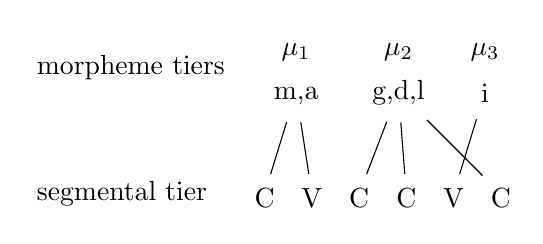
\begin{tikzpicture}[shorten >=2pt,shorten <=3pt, draw=black!100]
	\def \rowthreeht{4.4cm}
	\def \rowtwoht{3.8cm}
	\def \twopointfive{4.1cm}
	%\def \weightstwo{3.75cm}
	\def \rowoneht{2.5cm}
	%\def \weightsone{1.25cm}
	%\def \basement{2cm}
	\tikzstyle{c-node}=[text height=8pt,text centered,inner sep=3pt,minimum size=10pt]
	\tikzstyle{m-node}=[text height=7pt,text centered,inner sep=3pt,minimum size=12pt]
	\tikzstyle{r-node}=[text height=10pt,inner sep=0pt,minimum size=10pt]
	%\tikzstyle{d-node}=[text height=6pt,text centered,inner sep=0pt,minimum size=12pt]
	\tikzstyle{annot}=[text width=25ex,align=left]
	% labels
	\node[annot] (mtierstop) at (0cm,\twopointfive) {morpheme tiers};
	\node[annot] (segtier) at (0cm,\rowoneht) {segmental tier};
	%\node[annot] (mtiersbot) at (0cm,\basement) {};
	
	% surface layer
	\node[r-node] 	(r0)	at (1.0cm,\rowoneht)		{C};
	\node[r-node] 	(r1)	at (1.6cm,\rowoneht)		{V};
	\node[r-node] 	(r2)	at (2.2cm,\rowoneht)		{C};
	\node[r-node] 	(r3)	at (2.8cm,\rowoneht)	 	{C};
	\node[r-node] 	(r4)	at (3.4cm,\rowoneht)	 	{V};
	\node[r-node] 	(r5)	at (4.0cm,\rowoneht)	 	{C};
	
	% hidden-layer elements
	\node[r-node] 	(m0)	at (1.4cm,\rowthreeht)		{$\mu_{1}$};
	\node[r-node] 	(m1)	at (2.7cm,\rowthreeht)		{$\mu_{2}$};
	\node[r-node] 	(m2)	at (3.8cm,\rowthreeht)		{$\mu_{3}$};

	% hidden layer
	\node[c-node] 	(m3)	at (1.4cm,\rowtwoht)		{\/m,a\/};
	\node[c-node] 	(m4)	at (2.7cm,\rowtwoht)		{\/g,d,l\/};
	\node[c-node] 	(m5)	at (3.8cm,\rowtwoht)		{\/i\/};
		
	\path
		(m3)	edge	node	{}	(r0)
		(m3)	edge	node	{}	(r1)
		%
		(m4)	edge	node	{}	(r2)
		(m4)	edge	node	{}	(r3)
		(m4)	edge	node	{}	(r5)
		%
		(m5)	edge	node	{}	(r4);
		
	\end{tikzpicture}
	%\label{subfig:nonlinear}
	}

	\subfigure[\fontsize{11pt}{12pt}\selectfont Linear approach\label{subfig:linear-1}]{
	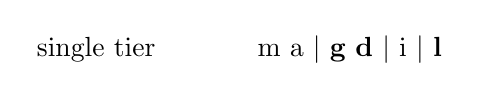
\begin{tikzpicture}[shorten >=1pt,draw=black!100]
	\vspace{50pt}
	\def \floor{0cm}
	\tikzstyle{f-node}=[text centered,inner sep=0pt] %text centered]
	\tikzstyle{annot}=[text width=34ex,align=left]
	% labels
	\node[annot] (floorlabel) at (0cm,\floor) {single tier};
	
	% surface layer
	\node[f-node] 	(f0)	at (1.4cm,\floor)			{m\,\,a\,\,$|$\,\,\textbf{g}\,\,\textbf{d}\,\,$|$\,\,i\,\,$|$\,\,\textbf{l}};
	\end{tikzpicture}
%\label{subfig:linear}
}
\caption{Multiple tiers vs. a single tier for morphological analysis}
\label{fig:nonlinear}
%\vspace{-20pt}
%\vspace{1pt}
\end{mdframed}
\end{figure}

%Notice that $\mu_2$, the consonantal root, is discontinuous; it is
%interrupted by $\mu_3$. 
%This autosegmental account of the 
By contrast, the analysis in figure~\ref{subfig:linear-1} is the \emph{linear} counterpart to the autosegmental  (or multilinear) analysis in figure~\ref{subfig:nonlinear-1}
If a model should have only one tier, as in 
figure~\ref{subfig:linear-1}, there would be no way of representing the
unity of $\mu_2$, i.e., the fact that \textit{g}, \textit{d}, and \textit{l}
all belong to the same morphological unit. Observations such as these motivate this thesis's two principal concepts: \emph{nonlinearity} and \emph{nonsequentiality}. We will define these concepts now and revisit them further in subsequent chapters. 
	\medskip
	\begin{definition}\label{def:nl}{\textbf{Nonlinearity}}: %A model is \emph{nonlinear} 
	A model is \textbf{nonlinear} if each of its morphs occupies a tier that is \emph{not} the phonological tier.
	%Morphs, i.e., units of morphological structure, must be separate from the surface (or phonological) tier. \end{definition} %, i.e., as residing on tiers distinct from the phonological tier. %eparately for m  as being separate from (or outside of) the the phonological (or segmental) tier.  % is a property wherein morphs are represented as being separate from the segmental tier.
	\end{definition}
	\begin{definition}\label{def:ns}{\textbf{Nonsequentiality}}: %is a property such that each morph tier (or node) is orthogonal to all other morph tiers.
	%---i.e., independent of---all other morph tiers. 
	A model is \textbf{nonsequential} if \textbf{no two morphs} occupy the \emph{same} tier. This is to say that all morphs are independent, i.e., that there are no morph-to-morph connections.
	\end{definition}
	\medskip
I propose that these two properties are the essential properties that enable autosegmental morphology to handle nonconcatenative morphology. The main idea of this thesis is that these two properties must be present in any model in order for it to be capable of handling (or learning) nonconcatenative morphology.  We will later revisit the idea stated here as proposition~\ref{prop:nlns} (see in particular section~\ref{sec:framework-intro}).
\begin{proposition}\label{prop:nlns}
%A model of morphology can handle nonconcatenative morphology if and only if it satisfies both \textbf{nonlinearity} and \textbf{nonsequentiality}.
A model of morphology can handle nonconcatenative morphology if it satisfies both \textbf{nonlinearity} and \textbf{nonsequentiality}.
\end{proposition}
%\pex~ Two essential properties  %\ex \label{ex:properties}\begin{xlist}
%	\a {\textsc{Nonlinearity}}: Morphemes are represented as being separate from the segmental tier.
%	\a {\textsc{Nonsequentiality}}: Each morpheme tier (or node) is orthogonal to---i.e., independent of---all other morpheme tiers.
%\xe
% \ex this is one 
%\marginpar{or multilinear}
%These criteria, or essential properties,
%%\textsc{nonlinear} and \textsc{nonsequential} 
%are basically binary variables; each \emph{must} be either True or False, and each can \emph{only} be True or False.  Each variable thus has two possible values,
%giving us four possible combinations of (non)linearity and (non)sequentiality: 
%\textbf{nonlinear nonsequential} (NLNS), \textbf{linear nonsequential} (LNS), 
%\textbf{nonlinear sequential} (NLS), and \textbf{linear sequential} (LS).

%[We should note that autosegmental morphology has other properties to
%constrain morphological structure, e.g., the well-formedness
%principle; at present, we are not concerned with capturing all aspects
%of autosegmental morphology, but instead in building a generic system
%to which one can later add linguistically motivated constraints.]

\section{Research Questions and Objectives}
%State primary research objective: 
%\subsection{Primary research objective}
The primary objective of this thesis is to demonstrate the idea expressed above as proposition \ref{prop:nlns} through a combination of rational argument and experimentation.
%that the crucial components of autosegmental theory, i.e., 
%those components that allow it to handle non-concatenative morphology, 
%This will be accomplished both through rational argument and experimentation.
The rational argument will consist in three main points.
First, the properties of nonlinearity and nonsequentiality are absolutely essential for dealing with nonconcatenative morphology.
Second, these properties are equivalent to the formal mathematical properties that define bipartite graphs. And third, this equivalence provides a foundation for the use of graphical learning models for the purpose of morphological learning. 
%The present study uses a graphical learning framework known as the multiple cause mixture model (MCMM) \citep{saund:94}. 
These points will be further fleshed out in chapters \ref{ch:lit-review}, \ref{ch:graph}, and \ref{ch:MCMM}. These chapters will expand and elucidate concepts originally presented in \citet{meyer-and-dickinson:2016}, an earlier version of the present work.
The experimental component of the dissertation consisted of the development and evaluation of
 \textbf{Multimorph}, a novel unsupervised morphology-learning system that is driven by a Multiple Cause Mixture Model (MCMM) \citep{saund:94} and embodies the three points stated above. 
	
	 \subsection{The Question of Features} There is a great deal of information tacitly present in a string of alphabetic symbols.
	 This is true regardless of whether the string is written, in which case the symbols are graphemes, or spoken,
	 in which case they are phonemes. In either case, the symbols are each drawn from an alphabet of size $N$ and arranged along a single axis.
By way of illustration, consider again the Hebrew word \textit{magdil}, but now specifically as a \emph{string of graphemes}: 
\begin{center}
%\textsf{m\,a\,g\,d\,i\,l}
%\textsf{magdil}
%\texttt{magdil}
%\textipa{magdil}
{\fontsize{12pt}{14pt}\selectfont magdil}
\end{center}
%from figure~\ref{fig:nonlinear}, but now we think of it specifically as the \emph{string of graphemes}.
%\begin{figure}[h]
%\vspace{12pt}
%	\centering
%	\begin{tikzpicture}[shorten >=2pt,shorten <=3pt, draw=black!100]
%	\Large
%	\def \rowoneht{0cm}
%	\def \rowtwoht{-0.8cm}
%	\tikzstyle{r-node}=[text height=10pt,inner sep=0pt,minimum size=10pt]
%	%\node[r-node] 	(r0)	at (0cm,\rowoneht)		{\textipa{magdil}};
%	\node[r-node] 	(r0)	at (0cm,\rowoneht)		{magdil};
%	%\node[r-node] 	(r0)	at (0cm,\rowoneht)		{s t o p};
%	%\node[r-node] 	(r0)	at (0cm,\rowtwoht)		{p o t s};
%	\end{tikzpicture}
%\end{figure} \\
%This row of six graphemes contains a vast amount of tacit information. For instance, suppose we had to represent the string \textit{magdil} not as sequence of alphabetic symbols, but as a series of simple declarative statements. We might come up with statements like the following: 
%%These statements might say that a certain character is present in the string, that one character precedes another character, that a particular character occurs at a particular position in the string, and so on, as in the following examples.
%\begin{itemize}
%  \item \textit{a} immediately follows \textit{m}, \textit{g} immediately follows \textit{a}, \textit{d} immediately follows \textit{g}, and so on. 
%  \item \textit{i} immediately precedes \textit{l}, \textit{d} immediately precedes \textit{i}, and so on.
%     \item \textit{g} follows both \textit{m} and \textit{a}, \textit{d} follows \textit{m}, \textit{a}, and 
%   \textit{g}; \textit{d} precedes both \textit{i} and \textit{l}, \textit{g} precedes \textit{d}, \textit{i}, and \textit{l}, and so on.
%   \item \textit{m} is the first character, \textit{a} is the second, \dots \textit{i} is the second-to-last character, and \textit{l} is the last character, and so on.
%   %\item \textit{l} is the sixth character, \textit{i} is the fifth, \textit{d} is the fourth, and so on.
%   \item \textit{m} precedes \textit{a}, \textit{m} precedes \textit{g}, \textit{m} precedes \textit{d}, \dots, \textit{m} precedes \textit{l}; \textit{a} precedes \textit{g}, \dots , \textit{a} precedes \textit{l}; and so on.
%   \item \textit{m} is present, \textit{a} is present, \textit{g} is present, and so on.
%   \item \emph{ad infinitum}
%\end{itemize}
%A string of alphabetic symbols tacitly conveys all of these facts and many more---perhaps infinitely more.
%Statements like these are essentially what we call \emph{features}.
%Each statement can be either true or false, which is to say that each feature is \emph{binary}, drawn from an alphabet of size $N = 2$.  
%Many machine learning models require that each input object or \emph{learning instance} (in our case, each \emph{word}) be represented as a vector of binary features, not alphabetic features. Moreover, all input objects (learning instances) must be described by the same feature set, and all feature vectors must be of the same length.
%One cannot, of course, have an infinite number of features, as feature vectors must be finite in length.
%Now, let $F$ be the infinite set of all possible features. In keeping with the spirit of my primary research objective, we shall assume that there exists at least one $\phi$ such that $\phi \subset F$, $\phi$ is finite, and $\phi$ allows a ULM system to learn a multilinear model of morphology. The objective here is to confirm this assumption, i.e., to find such a subset.
%There is a great deal of information tacitly present in a string of alphabetic symbols.
%This is true regardless of whether the string is written, in which case the symbols 
%are graphemes, or spoken, in which case they are phonemes. In either case, 
%the symbols are each drawn from an alphabet of size $N$ and arranged along 
%a single axis. % (say, the $x$ axis).
%By way of illustration, consider again the Hebrew word \textit{magdil}, but now specifically as a \emph{string of graphemes}.  In  
%from figure~\ref{fig:nonlinear}, but now we think of it specifically as the \emph{string of graphemes} 
%printed at the top of figure~\ref{fig:many-feats}. 
%By way of illustration, consider the string of graphemes
%displayed at the top of figure~\ref{fig:many-feats}.
%\begin{figure}[h]
%	\centering
%	\begin{tikzpicture}[shorten >=2pt,shorten <=3pt, draw=black!100]
%	\Large
%	\def \rowoneht{0cm}
%	\def \rowtwoht{-0.8cm}
%	\tikzstyle{r-node}=[text height=10pt,inner sep=0pt,minimum size=10pt]
%	%\node[r-node] 	(r0)	at (0cm,\rowoneht)		{\textipa{magdil}};
%	\node[r-node] 	(r0)	at (0cm,\rowoneht)		{magdil};
%	%\node[r-node] 	(r0)	at (0cm,\rowoneht)		{s t o p};
%	%\node[r-node] 	(r0)	at (0cm,\rowtwoht)		{p o t s};
%	\end{tikzpicture}
%\end{figure}
This six-grapheme string contains a vast amount of tacit information. For instance, 
suppose we had to represent the string \textit{magdil} not as sequence of alphabetic 
symbols, but as a series of simple declarative statements. We might come up with 
statements like the following: 
%in in figure~\ref{fig:many-feats}
%\begin{figure}[h]
%%line\hline
%%These statements might say that a certain character is present in the string, that one character precedes another character, that a particular character occurs at a particular position in the string, and so on, as in the following examples.
%\begin{center}
%\Large{magdil}
%\end{center}
%%\smallskip
\begin{itemize}
  \item \textit{a} immediately follows \textit{m}, \textit{g} immediately follows \textit{a}, \textit{d} immediately follows \textit{g}, and so on. 
  \item \textit{i} immediately precedes \textit{l}, \textit{d} immediately precedes \textit{i}, and so on. %What's more, we know that
   \item \textit{g} follows both \textit{m} and \textit{a}, \textit{d} follows \textit{m}, \textit{a}, and \textit{g}; \textit{d} precedes both \textit{i} and \textit{l}, \textit{g} precedes \textit{d}, \textit{i}, and \textit{l}, and so on.
   \item \textit{m} is the first character, \textit{a} is the second, \dots \textit{i} is the second-to-last character, and \textit{l} is the last character, and so on.
   %\item \textit{l} is the sixth character, \textit{i} is the fifth, \textit{d} is the fourth, and so on.
   \item \textit{m} precedes \textit{a}, \textit{m} precedes \textit{g}, \textit{m} precedes \textit{d}, \dots, \textit{m} precedes \textit{l}; \textit{a} precedes \textit{g}, \dots , \textit{a} precedes \textit{l}; and so on.
   \item \textit{m} is present, \textit{a} is present, \textit{g} is present, and so on.
   \item \emph{and so on \dots}
\end{itemize}
%\begin{itemize}
%  \item \textit{\textipa{a}} immediately follows \textit{\textipa{m}}, \textit{\textipa{g}} immediately follows \textit{\textipa{a}}, \textit{\textipa{d}} immediately follows \textit{\textipa{g}}, and so on. 
%  \item \textit{\textipa{i}} immediately precedes \textit{\textipa{l}}, \textit{\textipa{d}} immediately precedes \textit{\textipa{i}}, and so on. %What's more, we know that
%   \item \textit{\textipa{g}} follows both \textit{\textipa{m}} and \textit{\textipa{a}}, \textit{\textipa{d}} follows \textit{\textipa{m}}, \textit{\textipa{a}}, and \textit{\textipa{g}}; \textit{\textipa{d}} precedes both \textit{\textipa{i}} and \textit{\textipa{l}}, \textit{\textipa{g}} precedes \textit{\textipa{d}}, \textit{\textipa{i}}, and \textit{\textipa{l}}, and so on.
%   \item \textit{\textipa{m}} is the first character, \textit{\textipa{a}} is the second, \dots \textit{\textipa{i}} is the second-to-last character, and \textit{\textipa{l}} is the last character, and so on.
%   %\item \textit{\textipa{l}} is the sixth character, \textit{\textipa{i}} is the fifth, \textit{\textipa{d}} is the fourth, and so on.
%   \item \textit{\textipa{m}} precedes \textit{\textipa{a}}, \textit{\textipa{m}} precedes \textit{\textipa{g}}, \textit{\textipa{m}} precedes \textit{\textipa{d}}, \dots, \textit{\textipa{m}} precedes \textit{\textipa{l}}; \textit{\textipa{a}} precedes \textit{\textipa{g}}, \dots , \textit{\textipa{a}} precedes \textit{\textipa{l}}; and so on.
%   \item \textit{\textipa{m}} is present, \textit{\textipa{a}} is present, \textit{\textipa{g}} is present, and so on.
%   \item \emph{and so on \dots}
%\end{itemize}
%\hline
%\end{tikzpicture}
%\caption{Innumerable possible features.}
%\begin{tikzpicture}
%\label{fig:many-feats}
%\end{figure}
%A string like \textit{magdil} tacitly conveys all of these facts and many more---perhaps 
%infinitely more. 
All of these statements, as well as many others,
are tacitly expressed in the string \textit{magdil}.

What we call \emph{features} are essentially true-or-false statements like those listed above.
% ones in figure~\ref{fig:many-feats}.
%Each statement can be either true or false, which is to say that each feature is \emph{binary}, 
%drawn from an alphabet of size $N = 2$.  
Many machine learning models require that each input object or \emph{learning instance} 
(in our case, each \emph{word}) be represented as a vector of \emph{binary} features rather than alphabetic 
features. Moreover, all input objects (learning instances) must be described by the same feature 
set, and all feature vectors must be of the same length.
One cannot, of course, have an infinite number of features, since feature vectors must have a definite length.
One must therefore choose a particular subset of all possible features. The problem of choosing a likely subset constitutes one of
this dissertation's main research questions, and we
%In \ref{ch:intro}, we mentioned the problem of choosing one finite subset of features from an infinite number of possible features.
address it further in chapter~\ref{ch:experi}, where we will glean some insight 
by considering feature categories that 
are significant to computer vision, particularly \emph{invariant} and \emph{variant} features. I will argue that the distinction between these two categories is also important to the unsupervised learning of morphology.
% with an eye to better understanding the sort of features that are valuable to the unsupervised learning of morphology. 
%The idea is that 
%the task of clustering objects, i.e., discerning what makes two objects similar and what makes them different,
%and figuring out which objects to group together and which to separate, is a very general problem. And thus the
%same types of features should apply to different types of objects.
%These categories are \textit{variant} features and \textit{invariant} features. 
%>>>
%We will focus in particular on \emph{invariant} and \emph{variant} features. The distinction between these two categories is highly significant in
%computer vision and its various subfields. For the purposes of this dissertation, we hypothesize that this distinction is
%also important to unsupervised morphological learning. 


\subsection{The Question of Data Representation} 
 %emph{representation} of the input data,
In extracting features from the original data (a list of words), one alters the dataset. Different feature categories emphasize different kinds of information. But the raw material for feature extraction is in any case the original word list, and thus the way in which the words represented in the original dataset plays its own role in shaping features. 
By \emph{representation}, we refer mainly to the alphabet---the
particular set of symbols---from which the strings (i.e., words) of the input wordlist 
are composed.  A word is fundamentally something spoken, i.e., a sequence of sounds, and thus in order to write the word down, one must devise a way to represent the spoken phenomenon on paper. Like feature-set design, this is a means of emphasizing some information at the expense of other information. All else being equal---that is, even if the feature categories are the same---different modes of data representation will produce different features.  
In the present work, three manners of data representation were tested, each presenting 
different information. 

The question of how the input data should be represented is an important one in morphological 
learning because there are often 
a variety ways to represent linguistic data in text form. 
For instance, Japanese can be written in written in \textit{kanji} or 
\textit{kana} characters. The former are entirely logographic, as they 
have been borrowed directly from the Chinese \textit{Han} script, 
and as such, they are not connected to speech sounds in any way. The latter, by contrast,
represent syllables of spoken Japanese. That is, each single \textit{kana} 
character represents both a consonant and a vowel.  (Japanese syllables generally consist of a consonant onset and a vowel nucleus.)  Japanese can also be represented via alphabetic systems, which includes several systems of Romanization as well as scientific phonetic transcription systems such as the International Phonetic Alphabet (IPA).  One might reasonably ask how these various ways of representing Japanese as text might influence the unsupervised learning of Japanese morphology.

%There are indefinitely many ways to represent any language. 
%combination of this two. \textit{Kanji} are logographic characters borrowed directly from the Chinese \texit{Han} script, whereas \textit tAs logographic characters, they are not connected to speech sounds. Japananese   characters and ar chaSome modes of representation 
%are more transcriptional, 
%and others lean toward the orthographic. Some might go to great lengths to capture every phonological and morphophonemic alternation, while others might not express 
%any alternations. Still others might express graphemic alterations; for example, 
%some scripts have different shapes for some letters when the occur word-finally. 
%Some scripts might represent some phonological alternations, but not others, 
%perhaps because those alternations are perceived as more salient than others.
Like that of Japanese, the orthography of Hebrew has a long and rich history. Unlike Japanese, however, Hebrew has never been represented in a non-alphabetic script. Indeed, the ancient Hebrew alphabet was essentially the Phoenician alphabet, the world's first alphabetic writing system and the progenitor of all the alphabets that would in emerge in Europe and the Near East. Still, Hebrew orthography is by no means a straightforward matter, as we shall see in chapter~\ref{ch:experi}.
This dissertation tests three different modes of representing Hebrew as text:
\begin{enumerate}[itemsep=0pt]
\item Transcriptions that mark the primary stress in words
\item Transcriptions without stress markings 
\item Standard Hebrew orthography 
\end{enumerate} 
The third category---the standard orthography---is significant because standard Hebrew 
orthography lacks symbols reserved for vowels. Its alphabet consists only of consonants.\footnote{Some 
consonants can be used to represent vowels, namely the Hebrew equivalents of \textit{w} 
(pronounced as [v] in Modern Hebrew), \textit{y}, and \textit{h}. Even so, these symbols 
are still fundamentally consonants. This and other matters of Hebrew orthography 
will be discussed in chapter~\ref{ch:experi}.} An earlier version of the present work, 
\citet{meyer-and-dickinson:2016}, considered only standard Hebrew orthography. 
We therefore depart from this earlier work in a major way in the present study by including the transcriptional data. 

I initially hypothesized that models induced from the orthographic 
data would be the worst-performing ones. My reasoning was that any orthographic system without dedicated vowel symbols would necessarily let at least some morphologically salient information go unexpressed. I reasoned that this should be especially true in the case of Hebrew, as vowels appear to be especially salient to its morphology. %vowels %appear especially true in the case of Hebrew,  and second, vowels must be particularly important to 
%Hebrew because 
The derivational morphology of Hebrew is famously nonconcatenative, consisting in the interleaving of consonantal 
roots and vowel patterns. The experimental results, however, proved to be somewhat surprising, 
as we shall see in chapter~\ref{ch:results}.
% morphology consist missing out on a great deal of valuable information  It seemed that a vowel-less spelling system would since it seems so obvious that by lacking vowels, it is lacking set wi particularly note this study is noteworthy because the Hebrew alphabet has no vowelsinv take on a different shape word-finally. to a great   to a greater e  The question of data representation determines the raw material from which features are constructed, touches on a number concern the role of the input data in morphological learning, the distinction between information quantity and quality in the input data, as well the influence of 

%transcriptional representations. These differed only in that one marked stress and the other did not. (i.e., all vowels of the t (TS and TR, respectively); The third was \emph{orthographic}, comprising 
%the letters of the standard Hebrew alphabet mapped onto ASCII characters.
%%(\textbf{\text{T}^{S}); another transcriptional, but without stress (\textbf{\text{T}^{R}), and the third orthographic (\textbf{O})ransliterated to ASCII characters in the Hebrew Treebank \citep{simaan-et-al:2001}
%TS is the Berman Longitudinal Corpus's transcriptional system, 
%and TS is that same system with the stress markings removed. 
%%Its alphabet is thus BLC's 
%%transcriptional system, which we discussed above in section. % \ref{sec:transcription}.
%The information contained in O is differs both qualitatively and quantitatively from information contained in the T datasets  
%Arguably, T contains more information than O,
%since T represents each of Modern Hebrew's five vowels in such a way that each 
%vowel sound not only has a symbol, but its own
%has its own exclusive symbol 
%exclusive symbol.

%The features are extracted from raw-text data, wherein Hebrew words are represented as strings of alphabetic symbols, and the symbols are drawn from a particular alphabet. Now, it so happens that we have more than one alphabet at our disposal, and thus more than one way to represent the input data. These alphabets are the following:
%	\begin{enumerate}
%		\item \textbf{Modern Hebrew standard orthography}, as transliterated to ASCII characters in the Hebrew Treebank \citep{simaan-et-al:2001}. In the orthography of Modern Hebrew, certain consonants are regularly appropriated to represent vowels. For example, the Hebrew letter
%		\textcjheb{w}, transliterated as \textit{w} in the Hebrew Treebank, is by default the consonant /v/, but it is also used to represent the vowels /o/ and /u/. In most syllables, however, the vowel is not represented at all. 
%		\item \textbf{Phonemic transcriptions}, i.e., phonemically transcribed words. I have extracted two lists of phonemically transcribed words from the Hebrew portion of the CHILDES database \citep{macwhinney:2000a}. 
%		 These lists are the same except that stress is marked in one, but not in the other.
%	\end{enumerate}
%	%The phonemic transcriptions amount to 12,494 words.
%	The question is which mode of representation yields better feature vectors. This is equivalent to asking which mode delivers the largest quantity of useful information and/or the smallest quantity of irrelevant information.
%	\paragraph{Mixing and Objective Functions.} The \textbf{mixing function} 
%is essentially a voting rule \citep{saund:94}. It prescribes the method whereby the 
%``votes'' of  hidden units are combined to turn a particular feature (i.e., surface unit) \textsc{on} or \textsc{off} (see section~\ref{sec:mixing-function}. The \textbf{objective function} measures the discrepancy---or, alternatively, similarity---between the surface units' activities and their target activities. 
%It thus drives the model's learning by way of trial and error. Objective functions can 
%be either positive or negative. Positive objective functions measure similarity and thus 
%need to be maximized. Negative objective functions measure error and thus need to be minimized (see section~\ref{sec:mcmm-learning}).

%I intend to experimented with two radically different mixing functions, 
%viz. one that combines hidden-unit activities linearly and one that combines them nonlinearly.
%%%(see section~\ref{sec:mixing-function}). 
%Similarly, I intend to try out 
%two radically different objective functions, namely 
%both a negative and a positive % one (see section~\ref{sec:mcmm-learning}).
%objective function. %(see section~\ref{sec:mcmm-learning}).
%Why: What does the mixing function do? What would happen if there were no mixing function? The mixing function maps the hidden-unit activities
%What does the objective function do? What would happen if there were no objective function? 
%If there were no objective function, there could be no learning. Learning proceeds by trial and error. 
%The objective function supplies the error.

\subsection{The Question of Evaluation}  One goal of unsupervised learning is to discover previously unknown categories \citep{parsons:2004}. This is especially true where the present study is concerned. Chapter~\ref{autonomous} argues that unsupervised morphological learners by nature learn \emph{autonomous} morphological units, i.e., units that reside in an independent between phonology and syntax. Such units have no meaning in and of themselves, as they exist independently of syntax and semantics. It is difficult to know going into an experiment what these intermediate categories should look like and what would make purported intermediate categories correct or incorrect. 

%going
%The previously unknown categories in this case are going to be morphological units of some kind.
%However, these units will not be conventional morphemes or morphosyntactic categories. 
%
%Instead, MCMM-generated clusters will correspond roughly to Aronoff's 
%\emph{morphomes} \citep{aronoff:1994}, which can be described as \emph{pre-morphosyntactic} units, i.e.,
%units that have been assembled from phonemes, but have not yet been assigned 
%a syntactic or semantic meaning. I shall use the term \emph{morph} instead of 
%\emph{morphome}, however, since MCMM-generated clusters may not correspond 
%precisely to morphomes in every case (see section~\ref{sec:targets}).

Thus, the evaluation itself presents an important research question, namely the 
question of how to evaluate the output of an unsupervised morphological 
clustering algorithm, particularly one that considers only features of \emph{word-internal form}, 
having no access to word-external morphosyntactic features, e.g., the person, number, 
and gender of surrounding words. In this thesis, therefore, I took a multi-faceted 
approach to the evaluation, that is, one composed of three complementary sub-approaches, 
namely a qualitative, an intrinsic, and an extrinsic component. The extrinsic evaluation 
in particular was designed to address the problems inherent in evaluating an unsupervised 
learning system. This consideration of evaluation as a research question in its own right is 
another point of departure from \citet{meyer-and-dickinson:2016}, which had no extrinsic 
evaluation component, but only an intrinsic component and a much smaller qualitative 
component than that of the present study. We will discuss the evaluation in chapter~\ref{ch:eval}.

%Thus, my system will not require morphological building blocks to have particular
%meanings. Instead, it 
%My system will thus look for \emph{pre-morphosyntactic} 
%units, i.e., ones assembled from phonemes, but not yet assigned 
%a syntactic or semantic meaning. In a larger pipeline, such 
%building blocks could serve as an interface between morphosyntax 
%and phonology. For instance, while an MCMM can find Hebrew's default 
%masculine suffix \textit{-im}, it cannot say whether it is
%masculine or feminine in a given word, as this suffix
%also occurs in idiosyncratic feminine plurals. The extrinsic part of the evaluation will examine my system's utility as a component within such a pipeline
%(see section~\ref{sec:paradigms}).
%\emph{morphs}. \marginpar{I have yet to introduce morphs, tho} We do not know 
%beforehand \emph{exactly} what these morphs ought to look like. Since we cannot know 
%the ``right answers'' before the experiments are run, there can be no clear gold 
%standard against which to evaluate the MCMM's output. 
%
%Thus, the evaluation itself presents an important research question, namely the question of how to evaluate the output of an unsupervised morphological clustering algorithm, particularly one that considers only features of \emph{word-internal form}, having no access to word-external morphosyntactic features, e.g., the person, number, and gender of  surrounding words. Such an algorithm will inevitably produce clusters that do not correspond to abstract morphosyntactic categories or conventional morphemes.
%which are fundamentally morphosyntactic in nature even though the correspondence between morphemes and abstract, or ``atomic,'' morphosyntactic categories is not always one-to-one.

\section{Organization}
The remainder of this thesis is organized as follows: In chapter~\ref{ch:lit-review}, 
I present a new framework for thinking about the unsupervised learning of morphology. 
This framework is original to this thesis and stems from the concepts of nonsequentiality 
and nonlinearity, introduced above as the essential prerequisites for modeling 
nonconcatenative morphology. Chapter~\ref{ch:graph} establishes the relationship 
between autosegmental morphology and graph theory, particularly \emph{bipartite} 
graphs. Chapter~\ref{ch:MCMM} then introduces and describes a particular bipartite 
graphical learning model, namely the Multiple Cause Mixture Model (MCMM). 
As mentioned above, this is the learning model I have chosen to drive Multimorph, 
the system developed in this dissertation. The first four chapters thus establish a logical 
chain linking autosegmental morphological theory to a particular unsupervised learning 
model, namely the MCMM, which serves as Multimorph's learning model. 

The remaining five chapters (chapters \ref{autonomous} through \ref{ch:conclusion}) 
are concerned with the evaluation of Multimorph. Chapter~\ref{autonomous} addresses 
the question of the sort of categories that Multimorph and other unsupervised morphological 
should be expected to learn, i.e., the sort of categories that one should look for in evaluating such 
systems. This is part of the question of evaluation introduced above. Chapter~\ref{ch:experi} 
%describes the experimental setup;
describes the choices for Multimorph's features and the preparation of its datasets, thus addressing the questions of features and data representation.
%describes the preparation of Multimorph's input
%that is, it describes the collection and preparation of the datasets 
%and the experimental variables, including the three modes of data representation and the 
%parameters for the feature sets.
 Chapter~\ref{ch:eval} completes this thesis's response to the 
``question of evaluation.'' It describes a dual-paradigm evaluation method consisting of 
both an intrinsic and extrinsic component. The extrinsic component in particular may be 
of interest to other ULM researchers as an alternative to conventional evaluation methods. 
The results are presented and discussed in chapter~\ref{ch:results}, and chapter~\ref{ch:conclusion} 
offers concluding remarks.
\chapter{A CONCEPTUAL FRAMEWORK FOR UNSUPERVISED MORPHOLOGICAL LEARNING}
\label{ch:lit-review}

\section{Introduction}
\label{sec:framework-intro}
\cite{mccarthy:1981} points out a fundamental flaw in linear, 
concatenative approaches to morphological analysis: 
Such approaches acknowledge only a single level of representation, 
namely that of the \emph{segmental string}, i.e., the level of minimal 
phonological segments (essentially phonemes).\footnote{McCarthy uses
 the term \emph{segment} in the phonological sense, i.e., a minimal unit of sound. 
Researchers in \ac{ULM}, however, generally use the word to 
refer to minimal morphological units, 
as in \textit{the problem of morphological segmentation}, for example.}
Because they are restricted to this single layer, they can only represent 
morphological groupings in one way, namely to insert delimiters of 
some sort 
into the very string under analysis. At any given
insertion point, moreover, such an approach can see only two (phonological) segments, namely the one immediately to the left and the one immediately to the right.
It thus
has no way to identify morphs that are made up of discontiguous phonemes.

\cite{mccarthy:1981} offers an alternative \emph{nonlinear} 
approach to grouping segments into morphs, one that liberates the 
representation of morphs from the segmental tier. McCarthy's formalism, 
\emph{autosegmental morphology}, is an extension of the autosegmental 
approach to phonology developed by \citet{goldsmith:1976} to account 
for nonlinear phonological phenomena. One such phenomenon, for instance, 
is \emph{tone spreading}, whereby the tone on one vowel spreads to other 
vowels, leapfrogging any intervening consonants. 
Goldsmith's solution was to introduce \emph{autosegmental} tiers 
(or planes) of representation that were independent of and external 
to the segmental tier---tiers that could thus ``see'' and access any 
phonological segment in the segmental tier, as well as any subsequence 
of segments, contiguous or discontiguous. The key was the nonlinearity 
(or multilinearity)
introduced by the multiple tiers and their separation both from each other 
and the segmental tier. 
McCarthy's insight was that this same nonlinear architecture could be 
applied to the problem of nonconcatenative morphology, particularly the 
root-and-pattern morphology of Semitic languages. 

I have devised a framework for comparing (and classifying)
previous approaches
the unsupervised learning of morphology. This framework is a classification 
system derived from the definitions of nonlinearity and nonsequentiality 
(see chapter~\ref{ch:intro}, definitions \ref{def:nl} and \ref{def:ns}) 
and the proposition that 
a model can learn nonconcatenative morphology if and only if it 
possesses both of these categories (chapter~\ref{ch:intro}, 
proposition~\ref{prop:nlns}). In particular, first observe that nonlinearity 
and nonsequentiality are negative concepts and thus suggest the existence 
of their positive counterparts, namely \emph{linearity} and 
\emph{sequentiality}. To facilitate the exposition of these concepts, we 
repeat the definitions of nonlinearity and nonsequentiality here and 
then define their complements, \emph{linearity} and \emph{sequentiality}.
	\begin{description}%\label{def:nl}
	%\begin{definition*}
	\item[{\textsc{Nonlinearity}}:]A model is 
	\textbf{nonlinear} if each of its morphs occupies a tier that is \emph{not} the phonological tier.
	%\end{definition*}
	%\begin{definition*}
	%\label{def:ns}
	\item[{\textsc{Nonsequentiality}}:]
	A model is \textbf{nonsequential} if \textbf{no two morphs} occupy the \emph{same} tier. This is to say that all morphs are independent, i.e., there are no morph-to-morph connections. 
	\end{description}
	\begin{definition}\label{def:l}{\textsc{\textbf{Linearity}}}:
	A model is \textbf{linear} if at least some of its morphs occupy the phonological tier.
	\end{definition}
	\begin{definition}\label{def:s}{\textsc{\textbf{Sequentiality}}}:
A model is \textbf{sequential} if two or more morphs occupy the \emph{same} tier.\footnote{In practice, `` two or more morphs'' is tantamount to saying ``all morphs,'' since it is hard to envision a scenario in which only a subset of morphs occupy their own tiers.} This is to say that there are connections between at least some pairs of morphs.
	\end{definition}

Proposition~\ref{prop:nlns} in chapter~\ref{ch:intro} conditions an algorithm's ability to model nonconcatenative morphology on the \emph{conjunction} of nonlinearity and nonsequentiality. That is, 
\begin{quote}\noindent
A model of morphology can represent nonconcatenative morphology if it is nonlinear \emph{and} nonsequential.
\end{quote}
Thus, the desired category is the \emph{intersection} of the basic nonlinear and nonsequential categories, and because it is the desired category, it has to be a category in our conceptual framework.
%It stands to reason that the other categories would be related to this desired category. In par
The other categories are similarly derived by taking pairwise intersections of the basic categories outlined above, as shown in figure~\ref{fig:intersections}.
\begin{figure}[!h]
\centering
\fbox{\begin{minipage}{9cm}
\centering
\textbf{Nonlinear-nonsequential} $=$ nonlinear $\cap$ nonsequential \\
\textbf{Nonlinear-sequential} $=$ nonlinear $\cap$ sequential \\
\textbf{Linear-nonsequential} $=$ linear $\cap$ nonsequential \\
\textbf{Linear-sequential} $=$ linear $\cap$ sequential
\end{minipage}}
\label{fig:intersections}
\caption{Four-category framework.}
\end{figure}
The resulting framework thus consists of two orthogonal axes, each representing one of two binary distinctions,
namely ``linear vs. nonlinear'' and ``sequential vs. nonsequential." The following sections will discuss each of these categories
in turn, citing examples 
for each. 

%will use the term
%\textbf{nonlinear} (NL) to refer to learning
%models (or algorithms) one
%or more hidden layers to encode the
%morphological structure.
%We use the term \emph{nonlinear} in the sense of \citep{mccarthy:1981, goldsmith:1976}, i.e., 
%to describe learning models that incorporate more than one tier of representation, i.e., more than 
%just the words (segmental strings) themselves.
%Proposition \ref{prop:nlns} asserts that \emph{both} nonlinearity \emph{and} nonsequentiality
%must be present in a model if it is to capable of modeling nonconcatenative morphology.
%A model of morphology can represent nonconcatenative morphology if it is nonlinear and nonsequential.
% In other words, the category of models capable of the learning nonconcatenative 
% morphology is  the intersection of the (more general) nonlinear and 
% sequential categories. Thus, one of our framework's categories has to be 
% \textbf{nonlinear-nonsequential}. Indeed, this is the ``desired'' category, 
% so to speak, the category whose members are intrinsically capable of modeling/learning
% nonconcatenative morphology. 
 
% The other categories are likewise intersections
% of the basic categories outlined above.  They are derived as follows: 
% 
% For instance, another category is \textbf{nonlinear-sequential}, 
% or the intersection of the nonlinear and sequential categories. The remaining two categories, 
% \textbf{linear-nonsequential} and \textbf{linear-sequential} are analogously defined. The four categories are summarized in figure~\ref{fig:intersections}:



%\fbox{\begin{minipage}{9cm}
%\centering
%\textbf{Nonlinear-nonsequential} $=$ nonlinear $\cap$ nonsequential \\
%\textbf{Nonlinear-sequential} $=$ nonlinear $\cap$ sequential \\
%\textbf{Linear-nonsequential} $=$ linear $\cap$ nonsequential \\
%\textbf{Linear-sequential} $=$ linear $\cap$ sequential
%\end{minipage}}

% derived from the concepts \emph{nonlinearity} and 
%\emph{nonsequentiality}  and their respective complements 
%\emph{linearity} and \emph{sequentiality}. 
% We can think of the terms \emph{nonlinear} and \emph{nonsequential} as labels 
%for basic categories of models, namely the those that have the 
%property \emph{nonlinearity} and those that have the property 
%\emph{nonsequentiality}, respectively. Recall proposition \ref{prop:nlns}, 
%which posits that \emph{both} nonlinearity and nonsequentiality must be 
%present in a model if it is to be able to handle nonconcatenative morphology. 
%In other words, a model must belong to the \emph{intersection} of the 
%nonlinear and nonsequential models; i.e., it must be a \textbf{nonlinear nonsequential} 
%model.  And indeed, ``nonlinear-nonsequential'' is one of the categories of our four-category 
%framework.  The other three are derived similarly:
 

%In particular, the ``negative'' properties \emph{nonlinearity} and \emph{nonsequentiality} 
%imply the existence of their ``positive'' counterparts, namely  \emph{linearity} and \emph{sequentiality}, respectively, which correspond to the basic-category labels \emph{linear} and \emph{sequential}. We thus define
%\emph{linearity} and \emph{sequentiality} as the opposites of \emph{nonlinearity} and \emph{nonsequentiality}, respectively.
%
%	\begin{definition}\label{def:l}{\textsc{Linearity}}: %A model is \emph{nonlinear} 
%	Morphs are \emph{not} separate from the phonological tier. \end{definition}
%	\begin{definition}\label{def:s}{\textsc{Sequentiality}}:
%	Not all morph tiers are orthogonal to the other morph tiers
%	\end{definition}
% Proposition \ref{prop:nlns} states that \textbf{nonlinear nonsequential} needs to be one of framework's categories, and it is obtained by taking the intersection of the basic categories \emph{nonlinear} and \emph{nonsequential}. We derive the other categories by taking analogous intersections of basic categories, as follows:
%\begin{itemize}
%\item \textbf{Nonlinear-nonsequential} $=$ nonlinear $\cap$ nonsequential
%\item \textbf{Nonlinear-sequential} $=$ nonlinear $\cap$ sequential
%\item \textbf{Linear-nonsequential} $=$ linear $\cap$ nonsequential
%\item \textbf{{Linear-sequential} $=$ linear $\cap$ sequential
%\end{itemize}
%The linear-sequential category is the intersection of the linear and sequential basic categories; the nonlinear-sequential category is 

%The resulting framework thus consists of two orthogonal axes, each representing one of two binary distinctions,
%namely ``linear vs. nonlinear'' and ``sequential vs. nonsequential." 
%We use the term \emph{nonlinear} in the sense of \citep{mccarthy:1981, goldsmith:1976}, i.e., 
%to describe learning models that incorporate more than one tier of representation, i.e., more than 
%just the words (segmental strings) themselves.

%We thus use the term \emph{linear} in the sense of `one-dimensional' (i.e., in opposition to \emph{nonlinear}). 
%In particular, we use it to label learning models that  I in the sense that opposes our sense of nonlinear, i.e., 
%opposing categories to a pair of opposing categories; the first is learning models along two 
%orthogonal axes consists of four categories, namely  in two pairs of opposing categories, namely 
%``linear vs. nonlinear" and ``sequential vs. nonsequential." 
%We cross-combine these categories 
%to create a $2\times2$ grid, the cells of which represent create a total of four categories. 
%The first is the``linear vs. nonlinear" distinction of \citep{mccarthy:1981, goldsmith:1976} 
%to categorizing existing approaches in \ac{ULM}.


% in the
%surface layer, whereas 
%, the layer of the graphemes/phonemes.
% Here, \textit{hidden layer} is conceptually related to McCarthy's
% \textit{autosegmental tier}, but the two terms are not necessarily
% equivalent formally.  
%The term 
%\textbf{linear} (L), i.e., \emph{linear} in the sense of `one %(cf. ``one-dimensional'') 
%will serve as the label for 
%algorithms that operate solely within the layer of surface symbols.  %s the attempt to construct a representation of
%%morphological structure. 
%Typically, such algorithms denote the morph boundaries by inserting delimiters directly into segmental strings.
 %surface string with morpheme boundary symbols. %Note that we will be using \textit{linear} in the sense of `one dimensional,' rather than`in/like a (straight) line.'
% This definition is not unlike ``one dimensional," a fairly common
% sense of \textit{linear}.  We do not, however, use \textit{linear} to
% mean ``in/like a straight line."
%but one to be distinguished from ``in/like a straight line." As it is used in this paper, the term \textit{linear} s not related in any direct way to the notions of line and straightness.
%We do not, however, use \textit{linear} to mean ``in a straight line" or even ``like a straight line."
%

%In addition to the 
%\textit{linear} vs. {nonlinear} distinction, we will also introduce a distinction between each into
%\textbf{sequential} and \textbf{non-sequential}.
%%, obtaining four categories in all. We describe each below.
%An algorithm is sequential (S) if there is a necessary sequence to its morphological classification decisions, i.e., if, for any two decisions, one must precede the other.\footnote{By \textit{morphological 
%%if its makes morphological classification decisions depend on preceding or succeeding context, i.e., if there is a necessary sequence to its decisions.
%%presentational unit (or feature) depends on the immediately preceding unit(s). %the value of each representational unit is determined independently of all other units
%classification decision}, we mean any decision that maps an atomic representational unit (usually a character or a feature) to a morphological category. This definition includes simple ``split" decisions, where there are only two possible categories: ``part of the current morpheme" and ``part of the next morpheme."}
%On the other hand, in a non-sequential (NS) algorithm, all morphological classification decisions are made in parallel; i.e., the decisions are unordered.
%
% We thus have a total of four categories: linear sequential (LS),
% linear non-sequential  (LNS), non-linear sequential  (NLS), and finally
% non-sequential nonlinear (NLNS). In what follows, we describe each of these in turn.

%We will now discuss and exemplify each of these categories in turn.

%\section{linear sequential algorithms}
%\label{subsec:seq-lin}
%
%The linear sequential (LS) type of algorithm is depicted in figure~\ref{fig:seq-lin}. 
%LS algorithms consider only one layer of representation, namely the surface layer. They use no hidden layers, hence their linearity. The surface layer is made up of surface units, depicted as squares in figure~\ref{fig:seq-lin}.
%In LS algorithms, these squares are usually the characters themselves. 
%The task is to assign each character to a morphological class. Thus, in effect, 
%each square represents a morphological classification decision.
%The arrows indicate the sequential order of the algorithm's decisions. 
%The fact that there is such an order is the reason this type of algorithm is sequential.
%
%The first unsupervised morphological learners were LS algorithms. The earliest examples employed the Letter Successor/Predecessor Variety (LSV/LPV) measures \citep{harris:1955, harris:1967}. 
%Both measures are intended to indicate likely affixes.
%$\text{LSV}(x)$ is intended to find prefixes; given a string $x$ and corpus $W$, $\text{LSV}(x)$ returns the number of letter types that immediately follow $x$ whenever $x$ is word-initial in $W$.
%Letter Predecessor Variety (LPV) is essentially the same measure, except that its function is to find suffixes:
%%That is, LPV is simply LSV from the opposite direction: 
%It counts the grapheme types that immediately \emph{precede} $x$ whenever $x$ is \emph{word-final}.
%%$\text{LSV}(x,W)$ is used to find prefix-stem boundaries, and $\text{LPV}(x)$ to find stem-suffix boundaries. 
%
%% Stress sequential nature of algorithm
%By themselves, of course, LSV and LSP are merely counts; they must be ``unpacked" if they are to be used to discover legitimate morpheme boundaries.
%There are a few different techniques for doing this
%%using LSV/LSP to discover morpheme boundaries 
%\citep[see][]{hammarstrom:2011}; one is the ``peak and plateau" technique. The following describes the use of peak and plateau with LSV: 
%
%\begin{itemize}
%\item Given an $n$-length word $w$ whose graphemes are indexed from 0 to $n$, compute $\text{LSV}(w[0:i])$ for each $i$ in the range $[0, n)$.
%%in the range $[0, n)$. 
%\item Then, for each $i$ in $[0, n)$, insert a morpheme boundary after the substring $w[0:i]$ if and only if 
%\begin{equation*}
%\text{LSV}(w[0:i-1]) \le \text{LSV}(w[0:i]) \ge \text{LSV}(w[0:i+1]),
%\end{equation*}
%i.e., there is a local peak in the LSV sequence at index $i$.
%\end{itemize}
%
%It is not difficult to see the sequentiality and linearity of an LSV/LPV technique like peak and plateau.
%Such a technique is sequential because its decision making process is shaped by the sequential order of graphemes.
%An LSV technique, for example, must proceed left to right, one index at a time, because the LSV calculation at index $i$ depends on the preceding $i-1$ graphemes. Moreover, in peak and plateau, the question of whether or not to draw a morpheme boundary at index $i$ depends not only on the LSV at $i$, but also on the preceding and succeeding LSVs. LSV/LPV techniques are linear because they incorporate no hidden nodes and thus have no means of mediating associations between nonadjacent characters.
%
%The intuition behind the LSV/LPV method is that \emph{within} a morpheme, the identity of each letter depends on the letters that immediately precede or succeed it. But this is not the case \emph{between} morphemes. That is, the first letter of a morpheme is largely unpredictable given its preceding letters. Likewise, a morpheme's final letter is largely unpredictable given its succeeding letters. Thus, the number
% of possible letter types tends to increase sharply at the boundary between two morphemes.
%
%However, while morpheme boundaries generally coincide with high LVP/LSV counts, it is not necessarily true that a high LVP/LSV indicates a morpheme boundary.
%%LSV is not always a reliable indicator of morpheme boundaries. 
%\cite{hammarstrom:2011}, for example, provide LPV counts for the word \textit{disturbance}. 
%The highest LPV count of 25 
%%(i.e., 25 of the 26 possible letters in the English alphabet) 
%occurs between \textit{disturbanc} and \textit{e}.
%An LPV-based analysis would thus incorrectly identify \textit{e} as a suffix, a consequence of the ubiquity of \textit{e} as a stem-final letter in English spelling. 
%
%%Goldsmith
%Because of such problems, most linear sequential methods today have abandoned LSV/LPV, often in favor of frequency-based heuristics.
%\cite{goldsmith:2001}, for example, uses a score based on pointwise mutual information (PMI) to approximate the likelihood that a given character $n$-gram $c_{1}c_{2}...c_{n}$ is a morpheme. 
%%In particular, the PMI of the characters $c_{1}, c_{2}, ..., c_{n}$ is multiplied by the relative frequency of the $n$-gram $c_{1}c_{2}...c_{n}$. 
%\cite{goldsmith:2001} obtains candidate suffixes (intended for further processing) by taking the $n$-grams that are ranked highest according to this score.  
%%(i.e., the count of $c_{1}c_{2}...c_{n}$ divided by the total count of all $n$-grams). 
%
%%Moon
%\cite{moon-et-al:2009} apply tree data structures known as \textit{tries} to the task of finding stems and affixes, as have a number of other researchers \citep[e.g.,][]{schone-and-jurafsky:2000, monson:2004, argamon:2004}.
%Tries are useful for learning concatenative morphology because they compactly store recurring character sequences.
%%that are repeated a group of words. by sets of words beginning with the same character. 
%Each node in a trie represents a certain prefix string (with the root node representing the empty string), 
%and every path proceeding out from a node represents a possible succeeding character. 
%Thus, even though tries are tree data structures, they process data in a sequential manner. 
%They 
%%also represent morphological relationships linearly 
%are linear
%because they lack hidden nodes, and every path through a trie is deterministic. 
% \cite{moon-et-al:2009} depart from other trie-based methods in using document 
% boundaries to approximate semantic context. 
% This helps them weed out spurious analyses like the \textit{disturbanc}+\textit{e} 
% example above, but it does not change the fundamentally sequential and linear nature of their approach.
%%\citep{goldsmith:2001} or trie-based affix-finding
%%\citep{moon-et-al:2009}.
%% , for example, uses a score based on pointwise mutual information
%% (PMI) to approximate the likelihood that a given character $n$-gram
%% %$c_{1}c_{2}...c_{n}$ 
%% is a morphemic unit.
%% In particular, the PMI of the characters $c_{1},
%% c_{2}, ..., c_{n}$ is multiplied by the relative frequency of the
%% $n$-gram $c_{1}c_{2}...c_{n}$. \cite{goldsmith:2001} obtains candidate
%% suffixes by taking the $n$-grams that are ranked highest according to
%% this score.
%%(i.e., the count of $c_{1}c_{2}...c_{n}$ divided by the total count of all $n$-grams).  
%%
%%Moon
%% \cite{moon-et-al:2009} apply tries to the task of finding stems and
%% affixes, to store recurring character sequences.
%%, as have a number of other researchers. 
%% Tries are useful for learning concatenative morphology because they
%% compactly store recurring character sequences.
%%that are repeated a group of words. by sets of words beginning with the same character. 
%% Each node in a trie represents a certain prefix string (with the root node representing the empty string), 
%% and every path proceeding out from a node represents a possible succeeding character. 
%% Thus, even though tries are tree data structures, 
%%In all cases, the methods process data in a sequential manner and
%%lack hidden nodes for representing morphological relationships.
%% linearly, lacking hidden nodes.
%
%% ; one of them is the ``peak and plateau" technique, which works as follows:
%% \begin{itemize}
%% \item Given an $n$-length word $w$ whose graphemes are indexed from 0 to $n$, compute $\text{LSV}(w[0:i])$ for each $i$ in the range $[0, n)$. \item Insert a morpheme boundary after the substring $w[0:i]$ if and only if $\text{LSV}(w[0:i-1]) \le \text{LSV}(w[0:i]) \ge \text{LSV}(w[0:i+1])$, i.e., there is a local peak in the LSV sequence at index $i$.
%% \end{itemize}
%% Notice the sequential nature of this technique: each LSV calculation is determined solely by the immediately preceding string of graphemes. Note also its linearity: there is only a single layer of representation for both the grapheme sequence and the morphological analysis.
%
% \begin{figure}[tb]
% %\begin{minipage}{.3\textwidth}
% \begin{center}
% \begin{tikzpicture}[shorten >=1pt,->,draw=black!100,node distance = 1.3cm, auto]]
% 	\def \startnode{1.5cm}
% %	\def\secondrow{1.0cm}
% 	\tikzstyle{r-node}=[regular polygon sides=4,draw=black!100,thick,inner sep=0pt,minimum size=4mm]
% 	\tikzstyle{annot} = [text width=3cm]
% %	\tikzstyle{annot} = [text width=2.0cm, text centered]
% 	% labels
% %	\node[annot] (m-label) at (0,\thirdrow) {hidden-unit vector};
% %	\node[annot] (r-label) at (0, \secondrow) {prediction vector};
% %	\node[annot] (d-label) (0, 0) {observed data vector};
% 	% hidden layer
% 	\node[annot] (surface-label) at (0cm,0cm) {surface layer};
% %	\node[annot] (r-label) at (0, \secondrow) {prediction vector};
% %	\node[annot] (d-label) (0, 0) {observed data vector};
%	
% 	% surface layer
% 	\node[r-node] 	(r0)	at (\startnode,0cm)		{};
% 	\node[r-node] 	(r1)	at (2.5cm, 0cm)		{};
% 	\node[r-node] 	(r2)	at (3.5cm,0cm)	 	{};
% 	\node[r-node] 	(r3)	at (4.5cm,0cm) 		{};
% 	\node[r-node] 	(r4) 	at (5.5cm,0cm)   		{};
%	
% 	\path (r0)	edge	node	{}	(r1)
% 		(r1)	edge	node	{}	(r2)
% 		(r2)	edge	node	{}	(r3)
% 		(r3)	edge	node	{}	(r4);
% \end{tikzpicture}
% \end{center}
% \caption{linear sequential architecture.}
% %. Each representational unit depends on the preceding unit, and no unit exists outside of the surface layer.}
% \label{fig:seq-lin}
% \end{figure}
%
%% The intuition behind the LSV/LPV method is related to that behind the entropy-based methods in natural language processing:
%% %In fact, LSV generally increases/decreases as entropy increases/deceases: 
%% At any given point \emph{within} a morpheme, the next letter is fairly predictable, which generally coincides with a smaller number of succeeding letter types. But at the border between two morphemes, the next letter is much less predictable. This low predictability generally translates to a much larger set of options for the succeeding letter (i.e., a higher LSV). However, it out that LSV is not always a reliable indicator of morpheme boundaries. \cite{hammarstrom:2011}, for example, provide LPV counts for the word \textit{disturbance}. 
%% The highest count (25) 
%% %(i.e., 25 of the 26 possible letters in the English alphabet) 
%% occurs between \textit{disturbanc} and \textit{e}, An LPV-based analysis would thus yield an incorrect result in this case, a consequence of the fact that \textit{e} is such a ubiquitous word-final letter in English spelling. 
%
%%Goldsmith
%% More recent linear sequential methods
%% %have thus abandoned LSV/LPV, often in favor of
%% use frequency-based heuristics.  \cite{goldsmith:2001}, for example,
%% uses a score based on pointwise mutual information (PMI) to
%% approximate the likelihood that a given character $n$-gram
%% %$c_{1}c_{2}...c_{n}$ 
%% is a morphemic unit.
%% % In particular, the PMI of the characters $c_{1},
%% % c_{2}, ..., c_{n}$ is multiplied by the relative frequency of the
%% % $n$-gram $c_{1}c_{2}...c_{n}$. \cite{goldsmith:2001} obtains candidate
%% % suffixes by taking the $n$-grams that are ranked highest according to
%% % this score.
%% %(i.e., the count of $c_{1}c_{2}...c_{n}$ divided by the total count of all $n$-grams).  
%% %
%% %Moon
%% \cite{moon-et-al:2009} applies \textit{tries} to the task of finding stems and
%% affixes, to store recurring character sequences in the search for recurring character sequences.
%% % A number of other researchers have done the same.
%% % Tries are useful for learning concatenative morphology because they
%% % compactly store recurring character sequences.
%% %that are repeated a group of words. by sets of words beginning with the same character. 
%% % Each node in a trie represents a certain prefix string (with the root node representing the empty string), 
%% % and every path proceeding out from a node represents a possible succeeding character. 
%% % Thus, even though tries are tree data structures, 
%% In all cases, the methods process data in a sequential manner and
%% represent morphological relationships linearly, lacking hidden nodes.
%
%% , and every path through a trie is deterministic.
%% \cite{moon-et-al:2009} depart from other trie-based methods in using
%% document boundaries to approximate semantic context.  This helps them
%% weed out spurious analyses like the \textit{disturbanc}+\textit{e}
%% example above, but it does not change the fundamentally sequential and
%% linear nature of their approach.
%
%\section{Linear non-sequential algorithms}
%\label{subsec:nonseq-lin}
%In the linear non-sequential (LNS) type of algorithm, shown in figure~\ref{fig:nonseq-lin}, the representational units are generally not raw characters, but rather \emph{features}, i.e., binary variables representing the presence or absence of particular properties.
%%specifying whether or not a word has a certain property. 
%Features in non-sequential algorithms need not correspond to contiguous chunks of the original string; for example, features like the following are perfectly valid: ``\textit{t} precedes \textit{i} within $\delta$ characters" and ``\textit{t} precedes \textit{b} within $\delta$ characters," where the character pairs \emph{t..i} and \emph{t..b} are discontiguous as long as $\delta \ne 0$. Notice that such features cannot really be ordered; each is either \textsc{true} or \textsc{false} irrespective of order.
%All non-sequential algorithms---of which LNS algorithms are a subcategory---view a given word's features as being unordered, i.e., as being sequentially unrelated to each other. 
%But while LNS algorithms are non-sequential, they are linear because they incorporate no hidden units. Thus, even though an LNS algorithm's features may refer to discontiguous subsequences of characters, they are nonetheless restricted to representing only properties that are overtly present in the surface layer of characters. 
%
%One LNS example is the algorithm of \cite{poon-et-al:2009}, which uses log-linear models to induce morphological segmentations for Arabic and Hebrew. 
%Log-linear models are inherently non-sequential because they treat all features as independent, estimating a global joint probability for the entire bag of features. 
%%Sequential models, in contrast, estimate conditional probabilities based on sequential dependencies between features
%The algorithm of \cite{poon-et-al:2009} in particular searches for the set of parameters $\theta$ that maximizes the joint probability of a corpus $W$ and a morphological segmentation $S$, i.e., $P(W,S| \theta) = P(W|S; \theta) \cdot P(S| \theta)$. The segmentation $S$ is encoded by a set of features.
%%They generate candidate segmentations via Gibbs sampling. For each candidate, they extract a feature set
%
%%Log-linear models are well-suited for large numbers of arbitrarily defined features. 
%\cite{poon-et-al:2009} use two categories of features to encode a morphological segmentation: \textit{morpheme features} and \textit{morpheme context} features.
%The former encode (potential) morpheme types and their frequencies, e.g., \texttt{vlAv:5} and \texttt{w:31}. The 
%latter encode context types and their frequencies, where a \emph{context} consists of the $n$ characters preceding and succeeding a (potential) morpheme;
%%the character bigrams to the left and right of a potential morpheme, 
%e.g., the feature \texttt{\#w\_wn:12} would represent a context whose left side consists of \textit{w} preceded by the word boundary, whose right side is the bigram \textit{wn}, and whose frequency is 12. Importantly, these context features overlap. That is, in \texttt{\#w\_wn:12}, the \textit{w} and \textit{wn} are themselves morphemes whose contexts must be extracted.
%This feature overlap is made possible by the non-sequentiality of log-linear models.
%%is on the right, , respectively, and whose frequency of this particular context as 12.
%%s that the left context is the character \textit{w} preceded by the word boundary, the right context is the character bigram \textit{wn}, and the frequency of this particular context is 12).
%% and \textand the characters \textit{w} and \textit{n} are on the right potential morpheme\textit{w} on the left 
%%and the characters \textit{w} and \textit{n} on the right).
%%Note, however, that 
%
%Note, however, that log-linear models can handle much more non-sequentiality than this. Indeed, since a log-linear models is inherently non-sequential, it accommodate any sort of non-sequential feature. 
%%one can incorporate into log-linear model.
%%feature %or combination of feature types 
%%in a log-linear model.  
%One could, for example, incorporate
%features representing discontiguous bigrams,
%as already noted.
% One could also combine contiguous and discontiguous bigram features in the same feature set.
%%for example, have features representing both contiguous and discontinous bigrams in the same feature set.
%%However, one in principle could use any sort of feature in a log linear model, such as a feature type representing discontiguous bigrams, for example.
%%Each feature represents the both corpus and the segmentation jointly, and a fully specified set of features thus represents an entire segmented corpus;
%%but there is no limit on the variety or quantity of features one can incorporate into a log-linear model.
%% Why is a log linear model non-sequential?
%%Log-linear models are inherently non-sequential because they treat all features as independent, estimating a global joint probability for the entire bag of features. Sequential models, in contrast, estimate conditional probabilities based on sequential dependencies between features.
%% Why is a log linear model non-sequential?
%And yet it is not the nature of the features themselves that makes an algorithm non-sequential, but rather the lack of sequential relationships between features. The algorithm of \cite{poon-et-al:2009} is non-sequential because it does not process features in a particular order.
%% Why is Poon et al's algorithm linear?
%It is, however, linear because it incorporates no hidden units to mediate associations between features.
%
%%\cite{poon-et-al:2009} incorporate no latent variables, however. 
%%Their representation of morphological structure makes reference only to the the surface layer of graphemes. Their morpheme features are limited to  contiguous grapheme sequences, 
%%and their morpheme context features encode only extreme left and right contexts, 
%%thus assuming no internal boundaries (i.e., no morpheme interruptions).
%%%They generate candidate segmentations via Gibbs sampling, but, for an $n$-length word, they consider 
%%Because it only acknowledges the surface layer of text, the algorithm of \cite{poon-et-al:2009} can only isolate stems and affixes, not the discontiguous roots and patterns of Arabic and Hebrew.
%
%%\paragraph{inear non-sequential algorithms}
%%\label{subsec:nonseq-lin}
%%
%%Like LS algorithms, \textbf{linear non-sequential } (LNS) algorithms consist only of surface units, having no hidden layer, hence their linearity. LNS algorithms are different in that there are no dependencies between representational units. Each unit is independent of other units, hence their \textit{non-sequential} characterization.
%%%They consist only of surface units, hence their linearity. What sets LNS algorithms apart is the lack of dependencies between these units, h
%%%illustrated in figure~\ref{fig:nonseq-lin}, 
%%%there are no dependencies between representational units, but also no
%%%hidden units.
%%%; i.e., all representational units reside in the surface layer.  
%%As one example, \cite{poon-et-al:2009} use log-linear models to induce
%%morphological segmentations for Arabic and Hebrew. 
%%% Their algorithm
%%% searches for the set of parameters $\theta$ that maximizes the joint
%%% probability of a corpus $W$ and a segmentation $S$ (i.e., $P(W,S|
%%% \theta)$).
%%% = P(W|S; \theta) \cdot P(S| \theta)$.
%%%They generate candidate segmentations via Gibbs sampling. For each candidate, they extract a feature set
%%% Log-linear models are well-suited for large numbers of arbitrarily
%%% defined features.
%%% \cite{poon-et-al:2009} use morpheme features and morpheme context
%%% features.  The former category specifies a morpheme type and its
%%% frequency, e.g., \texttt{vlav:1} and \texttt{w:2}.  The latter
%%% category indicates the character bigrams to the left and right of a
%%% given morpheme, e.g., \texttt{\#w\_wn:1} (a word boundary followed by
%%% the character \textit{w} on the left and the characters \textit{w} and
%%% \textit{n} on the right).  Note, however, that one could use any type
%%% of feature or combination of feature types with a log-linear
%%% model. One could, for example, have features representing both
%%% contiguous and discontinues bigrams in the same feature set.
%%%
%%%However, one in principle could use any sort of feature in a log linear model, such as a feature type representing discontiguous bigrams, for example.
%%%Each feature represents the both corpus and the segmentation jointly, and a fully specified set of features thus represents an entire segmented corpus;
%%%but there is no limit on the variety or quantity of features one can incorporate into a log-linear model.
%%% Why is a log linear model non-sequential?
%%Log-linear models are non-sequential because they treat all features
%%as independent, estimating a global joint probability.
%%%for the entire bag of features.
%%% Sequential models, in contrast, estimate conditional probabilities
%%% based on sequential dependencies between features.
%%% Why is Poon et al's algorithm linear?
%%% \cite{poon-et-al:2009} incorporate no latent variables,
%%% %, however, 
%%% %Their representation of morphological structure makes 
%%% referencing only the the surface layer of graphemes.
%%% Their morpheme
%%% features are limited to contiguous grapheme sequences, and their
%%% morpheme context features encode only extreme left and right contexts,
%%% thus assuming no internal boundaries (i.e., no morpheme
%%% interruptions).  
%%Even though such a log-linear model allows for any type of feature,
%%including both contiguous and discontiguous $n$-grams,
%%%They generate candidate segmentations via Gibbs sampling, but, for an $n$-length word, they consider  
%%the algorithm ultimately can only isolate stems and affixes, because
%%it only acknowledges the surface layer of text.
%%%, and not discontiguous roots and patterns.
%%% of Arabic and Hebrew.
%
% \begin{figure}[tb]
% %\begin{minipage}{.3\textwidth}
% \begin{center}
% \begin{tikzpicture}[shorten >=1pt,->,draw=black!100]
% 	\def \startnode{1.5cm}
% %	\def\secondrow{1.0cm}
% 	\tikzstyle{r-node}=[regular polygon sides=4,draw=black!100,thick,inner sep=0pt,minimum size=4mm]
% 	\tikzstyle{annot} = [text width=3cm]
% 	% labels
% 	\node[annot] (surface-label) at (0cm,0cm) {surface layer};
% %	\node[annot] (r-label) at (0, \secondrow) {prediction vector};
% %	\node[annot] (d-label) (0, 0) {observed data vector};
%	
% 	% surface layer
% 	\node[r-node] 	(r0)	at (\startnode,0cm)		{};
% 	\node[r-node] 	(r1)	at (2.5cm, 0cm)		{};
% 	\node[r-node] 	(r2)	at (3.5cm,0cm)	 	{};
% 	\node[r-node] 	(r3)	at (4.5cm,0cm) 		{};
% 	\node[r-node] 	(r4) 	at (5.5cm,0cm)   		{};
%	
% %	\path (r0)	edge	node	{}	(r1)
% %		(r1)	edge	node	{}	(r2)
% %		(r2)	edge	node	{}	(r3)
% %		(r3)	edge	node	{}	(r4);
% \end{tikzpicture}
% \end{center}
% \caption{inear non-sequential architecture}
% 
% %. No dependencies exist between representational units, and no unit exists outside of the surface layer.}
% \label{fig:nonseq-lin}
% \end{figure}
%
%% \cite{poon-et-al:2009} use morpheme features and morpheme context
%% features.  The former category specifies a morpheme type and its
%% frequency, e.g., \texttt{vlav:1} and \texttt{w:2}.  The latter
%% category indicates the character bigrams to the left and right of a
%% given morpheme, e.g., \texttt{\#w\_wn:1} (a word boundary followed by
%% the character \textit{w} on the left and the characters \textit{w} and
%% \textit{n} on the right).  Note, however, that one could use any type
%% of feature or combination of feature types with a log-linear
%% model. One could, for example, have features representing both
%% contiguous and discontinues bigrams in the same feature set.
%
%
%\section{Sequential nonlinear algorithms}
%\label{subsec:seq-nonlin}
%% First, what sort of algorithms are sequential nonlinear?
%The sequential nonlinear (NLS) type of algorithm is illustrated in figure~\ref{fig:seq-nonlin}. 
%Note in particular the addition of a hidden layer, whose units (the circular nodes)
%represent the underlying sources of the surface data's implicit structure.
%%account for the surface %the surface units and thus take responsibility for the regularities ac
%%for 
%%algorithms differ from linear sequential ones in that 
%%they add a layer of hidden units for 
%%encoding 
%%take responsibility for generating the structure implicit
%%the regularities %, i.e., the implicit structure, 
%%in the surface layer and thus the
%%data.
%%These hidden units can be viewed as causing or generating the surface data.
%NLS algorithms are nonlinear because they incorporate a hidden layer.
%However, they are sequential because the hidden layer in an NLS algorithm is sequential; i.e., its component hidden units
%%hidden units
%are sequentially ordered.
%Since the surface units depend on the hidden units, the hidden layer imposes its sequential order on the surface layer. 
%%they have a certain each hidden unit depends on its predecessor hidden unit(s). 
%% I need to say what the nonlinear aspect brings to the table. If being nonlinear is beneficial, sequential nonlinear algorithms should be better than linear sequential ones. So what do sequential nonlinear algorithms have that linear sequential algorithms don't? How does being nonlinear help them?
%% First, what sort of algorithms are sequential nonlinear?
%
%%Sequential nonlinear (NLS) algorithms
%%%, illustrated in figure~\ref{fig:seq-nonlin}, 
%%differ from sequential
%%linear ones by adding a layer of hidden units for encoding the
%%structure of the surface layer.
%%This makes them nonlinear. 
%% They are still sequential, however, in that there are sequential
%% dependencies within the hidden layer.
%%; i.e., each hidden unit depends on its predecessor hidden unit(s).
%%The prototypical example of a sequential nonlinear model is the Hidden
%%Markov Model (HMM).  \cite{creutz-and-lagus:2005,
%%  creutz-and-lagus:2007} employ an HMM to induce a morphological
%%lexicon.
%The prototypical NLS model is the Hidden Markov Model (HMM). 
%\cite{creutz-and-lagus:2005, creutz-and-lagus:2007} employ an HMM to induce a morphological lexicon, i.e., a list of morpheme-like segments they call \textit{morphs}. 
%%, i.e., a list of morpheme-like segments.
%%that they call \textit{morphs}.
%%sorted in order of increasing morph length. 
%%They take a maximum a posteriori (MAP) approach.
%Their algorithm seeks to find the lexicon such that $P(lexicon|corpus)$ is maximized. Due to Bayes' theorem, this equates to finding the lexicon that maximizes $P(corpus|lexicon) \cdot P(lexicon)$. The probability $P(corpus|lexicon)$ is computed by an HMM. Each unit in this HMM's hidden layer can take on five possible values: \textit{prefix}, \textit{stem}, \textit{suffix}, \textit{word boundary}, and \textit{non-morpheme}. 
%Note how the first four relate sequentially to each other: prefixes must precede stems, stems must precede suffixes, and so on.
%%The observation sequence is a segmentation hypothesis, i.e., a candidate segmentation of the corpus into morphs. 
%%Candidate segmentations are generated independently of the HMM, as are the transition and emission probabilities. 
%%The HMM's role to find likely hidden state sequence, which is computed by the Viterbi algorithm, along with the probability $P(corpus|lexicon)$. 
%The hidden layer in this case serves to facilitate the search for the optimal lexicon 
%(i.e., segmentation) by providing a means of abstracting away from the literal surface characters.
%
%%The HMM's role is to evaluate each candidate morph sequence. 
%% took out the "h"
% \begin{figure}[tb]
% %\begin{minipage}{.3\textwidth}
% \begin{center}
% \begin{tikzpicture}[shorten >=1pt,->,draw=black!100]
% 	\def \rowtwoht{1.0cm}
% 	\def \rowoneht{0.0cm}
% 	\tikzstyle{m-node}=[circle,draw=black!100,thick,inner sep=0pt,minimum size=4mm]
% 	\tikzstyle{r-node}=[regular polygon sides=4,draw=black!100,thick,inner sep=0pt,minimum size=4mm]
% 	\tikzstyle{annot} = [text width=3cm]
% 	% labels
% 	\node[annot] (hidden-label) at (0cm,\rowtwoht) {hidden layer};
% 	\node[annot] (surface-label) at (0cm,\rowoneht) {surface layer};
%
% %	\node[annot] (d-label) (0, 0) {observed data vector};
%	
% 	% hidden layer
% 	\node[m-node] 	(m0)	at (1.5cm,\rowtwoht)		{};
% 	\node[m-node] 	(m1)	at (2.5cm,\rowtwoht)		{};
% 	\node[m-node] 	(m2)	at (3.5cm,\rowtwoht)	 	{};
% 	\node[m-node] 	(m3)	at (4.5cm,\rowtwoht) 		{};
% 	\node[m-node] 	(m4) 	at (5.5cm,\rowtwoht)   		{};
%	
% 	% surface layer
% 	\node[r-node] 	(r0)	at (1.5cm,\rowoneht)		{};
% 	\node[r-node] 	(r1)	at (2.5cm,\rowoneht)		{};
% 	\node[r-node] 	(r2)	at (3.5cm,\rowoneht)	 	{};
% 	\node[r-node] 	(r3)	at (4.5cm,\rowoneht) 		{};
% 	\node[r-node] 	(r4) 	at (5.5cm,\rowoneht)   		{};
%	
% 	\path (m0)	edge	node	{}	(m1)
% 		(m1)	edge	node	{}	(m2)
% 		(m2)	edge	node	{}	(m3)
% 		(m3)	edge	node	{}	(m4);
%		
% 	\path (m0)	edge	node	{}	(r0)
% 		(m1)	edge	node	{}	(r1)
% 		(m2)	edge	node	{}	(r2)
% 		(m3)	edge	node	{}	(r3)
% 		(m4)	edge	node	{}	(r4);
%			
% \end{tikzpicture}
% \end{center}
% \caption{Sequential nonlinear architecture}
% % . Sequential dependencies only exist between hidden units, 
% % not between the observed units of the surface layer. The hidden units ``cause" the surface units.}
% \label{fig:seq-nonlin}
% \end{figure}
%
%\section{Non-sequential nonlinear algorithms}
%\label{subsec:nonseq-nonlin}
%% Intro
% Like sequential nonlinear (NLS) algorithms, \textit{non}-sequential
% nonlinear (NLNS) algorithms incorporate a hidden layer whose units generate the observed
% units of the surface layer.
%The difference is that the hidden layer in an NLNS algorithm is \emph{non-sequential}; 
%i.e., the algorithm computes the values of all hidden units in parallel rather than in a sequence.
%The surface layer in a NLNS algorithm is also non-sequential.
% %dependencies.
% Thus, every unit---whether hidden or surface---is entirely independent
% within its own layer. Figure~\ref{fig:nonseq-nonlin} illustrates the NLNS framework; notice that no two nodes with the same layer are connected by an arc.
%This intra-layer independence allows a hidden unit to associate with
%any combination of surface units, whether contiguous or discontiguous
%%(see Figure \ref{fig:nonseq-nonlin}).
%
% \begin{figure}[tb]
% %\begin{minipage}{.3\textwidth}
% \begin{center}
% \begin{tikzpicture}[shorten >=1pt,->,draw=black!100] %,scale=.95]
% 	\def \rowtwoht{1.25cm}
% 	\def \rowoneht{0.0cm}
% 	\tikzstyle{m-node}=[circle,draw=black!100,thick,inner sep=0pt,minimum size=5mm]
% 	\tikzstyle{r-node}=[regular polygon sides=4,draw=black!100,thick,inner sep=0pt,minimum size=4mm]
% 	\tikzstyle{annot} = [text width=3cm]
% 	% labels
% 	\node[annot] (hidden-label) at (0cm,\rowtwoht) {hidden layer};
% 	\node[annot] (surface-label) at (0cm,\rowoneht) {surface layer};
%
% %	\node[annot] (d-label) (0, 0) {observed data vector};
%	
% 	% hidden layer
% 	\node[m-node] 	(m0)	at (2.5cm,\rowtwoht)		{};
% 	\node[m-node] 	(m1)	at (3.5cm,\rowtwoht)		{};
% 	\node[m-node] 	(m2)	at (4.5cm,\rowtwoht)	 	{};
% 	\node[m-node] 	(m3)	at (5.5cm,\rowtwoht) 		{};
%	
% 	% surface layer
% 	\node[r-node] 	(r0)	at (1.5cm,\rowoneht)		{};
% 	\node[r-node] 	(r1)	at (2.5cm,\rowoneht)		{};
% 	\node[r-node] 	(r2)	at (3.5cm,\rowoneht)	 	{};
% 	\node[r-node] 	(r3)	at (4.5cm,\rowoneht) 		{};
% 	\node[r-node] 	(r4) 	at (5.5cm,\rowoneht)   		{};
% 	\node[r-node] 	(r5) 	at (6.5cm,\rowoneht)   		{};
%	
% 	\path (m0)	edge	node	{}	(r0)
% 		(m1)	edge	node	{}	(r1)
% 		(m2)	edge	node	{}	(r3)
% 		(m1)	edge	node	{}	(r2)
% 		(m1)	edge	node	{}	(r4)
% 		(m3)	edge	node	{}	(r5);
%		
% \end{tikzpicture}
% \end{center}
% \caption{Non-sequential nonlinear architecture}
% %. Neither layer contains sequential dependencies; every unit is independent within its own layer. Each hidden unit is thus free to cause any combination of observed units.}
% \label{fig:nonseq-nonlin}
% \end{figure}
%
%The NLNS type can take many forms. 
%\cite{baroni-et-al:2002}, for example, detect implicit causal units by computing the Levenshtein alignments for pairs of words. 
%The Levenshtein algorithm finds the minimum number of edit operations 
%(typically allowing substitutions, deletions, and insertions) required to change 
%a \textit{source} word into a \textit{target} word.
%An alignment of the source and target characters is obtained as a by-product of computing the edit operations. 
%%In addition to edit distance and edit operations, the algorithm can align the characters of the source with those of the target word. 
%From the alignment, one can extract the (not necessarily contiguous) subsequence held in common by the two words.
%%One might view the common subsequence as suggesting a sin
%Thus, one may view the alignment as suggesting a single causal unit behind both occurrences of the subsequence, i.e., as a kind of implicit hidden unit, as it were.
%For example, the alignment in figure~\ref{fig:lev-align} implies a single cause behind both occurrences of the subsequence \textit{dbr}.
%Of course, a common subsequence does not necessarily indicate a morphological relationship; 
%consider, for instance, the English pair \textit{pork}/\textit{park}. 
%To avoid finding spurious relationships, 
%\cite{baroni-et-al:2002} compute a semantic similarity score based on mutual information, 
%combining it with an orthographic similarity score based on minimum edit distance.
%
% \begin{figure}[htb!]
% %\begin{minipage}{.3\textwidth}
% \begin{center}
% \begin{tikzpicture}[draw=black!100]
% 	%[shorten >=1pt,->,draw=black!100]
% 	\def \rowtwoht{1.5cm}
% 	\def \rowoneht{0.0cm}
% 	\tikzstyle{m-node}=[circle,draw=black!100,thick,inner sep=0pt,minimum size=6mm]
% 	\tikzstyle{r-node}=[circle,draw=black!100,thick,inner sep=0pt,minimum size=6mm]
% 	\tikzstyle{annot} = [text width=2.5cm, text centered]
% 	% labels
% 	\node[annot] (hidden-label) at (0cm,\rowtwoht) {target};
% 	\node[annot] (surface-label) at (0cm,\rowoneht) {source};
%
% %	\node[annot] (d-label) (0, 0) {observed data vector};
%	
% 	% hidden layer
% 	\node[m-node] 	(m0)	at (2.5cm,\rowtwoht)		{m};
% 	\node[m-node] 	(m1)	at (3.5cm,\rowtwoht)		{d};
% 	\node[m-node] 	(m2)	at (4.5cm,\rowtwoht)	 	{b};
% 	\node[m-node] 	(m3)	at (5.5cm,\rowtwoht) 		{r};
%	
% 	% surface layer
% 	\node[r-node] 	(r0)	at (2.5cm,\rowoneht)		{d};
% 	\node[r-node] 	(r1)	at (3.5cm,\rowoneht)		{i};
% 	\node[r-node] 	(r2)	at (4.5cm,\rowoneht)	 	{b};
% 	\node[r-node] 	(r3)	at (5.5cm,\rowoneht) 		{r};
%	
% 	\path (m1)	edge	node	{}	(r0)
% 		(m2)	edge	node	{}	(r2)
% 		(m3)	edge	node	{}	(r3);
%		
% \end{tikzpicture}
% \end{center}
% \caption{The minimum-edit-distance alignment for the Hebrew words \textit{dibr} `he spoke' and \textit{mdbr} `he is speaking'. The discontiguous root \textit{d.b.r } is discovered by aligning \textit{dibr} with \textit{mdbr} and extracting the common subsequence.}
% \label{fig:lev-align}
% \end{figure}
%
%
%Other authors simulate a nonlinear, multi-tier representation by separating the 
%learning process into two or more phases.
%The first phase classifies individual literal characters into abstract categories that are then used by a second phase (and perhaps subsequent phases) to perform other aspects of the analysis.
%Multiple phases occurring at different times can thus replicate the effects of multiple simultaneous levels of representation.
%This is the approach taken by \cite{rodrigues-and-cavar:2005} to induce the non-concatenative morphology of Arabic. 
%Their first phase identifies root radicals according to the statistical constraint-based method of \cite{elghamry:2005}. 
%For each word in their corpus, 
%they generate a set of candidate triliteral roots according to 
%constraints derived from the tendencies of Arabic roots as observed in corpora. 
%In particular, any 3-length subsequence is admitted into the candidate set 
%if and only if it satisfies both of the following:
%\begin{enumerate} 
%\item No two consecutive radicals may be separated by more than two characters.
%\item No more than four characters intervene between the first and third radicals.
%\end{enumerate}
%%\item ``The distance between the first and third radicals cannot be greater than five" \citep[][p. 3]{elghamry:2005}. 
%Then, a statistical score is computed for each candidate, and the one with the highest score is selected as the root.
%Once the roots---and thus the stems---have been isolated by the first phase, the second phase identifies the concatenative affixes through a separate methodology.
%
%% Goldsmith and Xanthos
%An alternative first-phase strategy can be found in \cite{goldsmith-and-xanthos:2009}, 
%who present methods for
%partitioning a phonemic inventory into a class of consonants and a class of vowels. 
%Their paper does not go into automatic morphological analysis, but it is not difficult to see how C and V classes could be useful to a multi-phase morphological analyzer.
%The first phase would partition the phonemic inventory and, for each word, label each phoneme/grapheme as either a consonant or vowel, thus creating a sort of CV skeleton similar to the segmental tier of autosegmental phonology.
%Subsequent phases would then use these CV skeletons to isolate roots, patterns, and other morphemes.
%%The second phase (and perhaps subsequent phases) would then use template to Such a template would be helpful to subsequent phases as they go about isolating the root, pattern, and other morphemes. 
%%To delimit distinct morphemes, the linear approach must 
%
%While the NLNS approaches described in this section provide a means for detecting discontiguous morphemes, they are not without their weaknesses. 
%% Baroni
%%% Mucho filtering
%The algorithm of \cite{baroni-et-al:2002} must filter out a large proportion of its input corpus, accepting only the words with relative frequencies of less than 0.01 percent; which are presumed to be content words.
%%% Arbitrary thresholds
%It also relies on arbitrary thresholds; e.g., the threshold for orthographic similarity measure (i.e., $1 - $ the normalized minimum edit distance) is set at 0.5, although there is no obvious reason why this should be so.
%Note also that behind this threshold is the assumption that morphologically related words share at least half of their characters, which is not necessarily true. Such an assumption would be especially problematic for highly agglutinative languages, 
%in which it is not uncommon for a stem to comprise a minority of a word's characters.
%Moreover, the Levenshtein edit-distance approach is only capable of comparing words pairwise, which only allows morphological relationships to be expressed on a pairwise basis. This is a consequence of the lack of an explicitly encoded hidden causal layer; an explicit (as opposed to implicit) hidden layer could easily mediate multi-way associations among surface layer components.                                   
%
%% Rodrigues and Cavar
%%% Only tri-literal roots
%Moreover, \cite{rodrigues-and-cavar:2005}, following \cite{elghamry:2005}, limit their algorithm's search to triliteral roots in order to reduce the problem's complexity, even though quadriliteral roots are not uncommon in Hebrew or Arabic.
%%% Reasonable constraints, but constraints nonetheless. A truly general algorithm wouldn't need constraints. 
%And while their two constraints on candidate-root generation are quite reasonable, these constraints are particular to the case of Semitic morphology, and thus they would not be required by a truly general algorithm.
%
%\cite{botha:blunsom:13} use mildly context-free grammars 
%with crossing branches to generate words with discontiguous morphemes. This approach
%is nonlinear because it utilizes multiple levels of structure in the form of a tree.
%The surface characters
%constitute the leaf nodes, which are the children of either the \emph{root} 
%or the \emph{template} node, which in turn are the children of the \emph{stem} 
%node, and so on.  It is nonsequential because the root and template nodes are unordered with respect to
%each other.
%
%\marginpar{Note some shortcoming.}
% In contrast [to the works discussed in this section], the Multiple Cause Mixture Model (MCMM) \citep{saund:94} is an NLNS algorithm that explicitly represents both surface and hidden nodes in a single graphical model. The MCMM is the focus of the next section.
 
% STARTHERE
 
%\section{Morphological Learning Frameworks}
%\label{sec:rel-work}
%\cite{mccarthy:1981} notes a fundamental flaw in linear, strictly concatenative approaches to morphological analysis: 
%Because such approaches acknowledge only a single level of representation, the segmental string, they are forced to represent within the same string both the linear order of phonemes and their grouping into morphemes. This effectively binds morphological grouping to the linear order of phonemes, leaving a linear analysis  
%with no straightforward means of identifying a discontiguous phoneme sequence as a unified morpheme.
%
%McCarthy thus offers an alternative \emph{nonlinear} formalism in 
%which morphemes are represented as nodes on \emph{autosegmental} tiers, 
%i.e., tiers that are separate from the segmental string, allowing
%associations between morphemes and phonemes to be independent of 
%phonemes' linear order. This framework turns out to be highly general, 
%for it uses the same formal machinery to model both 
%concatenative and non-concatenative processes; that is, it treats them as essentially 
%the same rather than fundamentally different.
%
%One can apply McCarthy's ``linear vs. nonlinear" conceptual framework to 
%categorizing existing approaches in ULM.
%In the following discussion, we
%use the term \textbf{nonlinear} (NL) as a label for algorithms that employ one
%or more \textit{hidden layers} to encode the structure of the
%\textit{surface layer}.
%We use \textbf{linear} (L) %(cf. ``one-dimensional'') 
%to label
%algorithms that reference only the surface layer of graphemes in the representation of
%morphological structure, e.g., by annotating the
%surface string itself with morpheme boundary symbols. Note that our sense of \textit{linear} 
%is similar to `one dimensional,' which is not necessarily the same as `in/like a (straight) line.'
%
%We further divide the categories
%\textit{linear} and \textit{nonlinear} each into
%\textbf{sequential} and \textbf{non-sequential} subcategories:
%%, obtaining four categories in all. We describe each below.
%An algorithm is sequential (S) if there is a necessary sequence to its morphological classification decisions, 
%i.e., if its decisions are ordered so that for every two decisions, one must precede the other.\footnote{By \textit{morphological 
%classification decision}, we mean any decision that maps an atomic representational unit (usually a character or a feature) to a morphological category. This definition includes simple ``split" decisions, where there are only two possible categories: ``part of the current morpheme" and ``part of the next morpheme."}
%On the other hand, in a non-sequential (NS) algorithm, all morphological classification decisions are made in parallel; i.e., the decisions are unordered.
%
% We thus have a total of four categories: sequential linear (SL),
% non-sequential linear (NSL), sequential non-linear (SNL), and finally
% non-sequential nonlinear (NSNL). In what follows, we describe each of these in turn.

%We will now discuss and exemplify each of these categories in turn.

\section{Sequential linear algorithms}
\label{subsec:seq-lin}

The sequential linear (SL) type of algorithm is depicted in figure~\ref{fig:seq-lin}. 
SL algorithms consider only one layer of representation, namely the surface layer. 
They use no hidden layers, hence their linearity. The surface layer is made up of surface units, depicted as squares in figure~\ref{fig:seq-lin}.
In SL algorithms, these squares are usually the characters themselves. 
The task is to assign each character to a morphological class. Thus, in effect, 
each square represents a morphological classification decision.
The arrows indicate the sequential order of the algorithm's decisions. 
The fact that there is such an order is the reason this type of algorithm is sequential.

 \begin{figure}[ht]
 \begin{mdframed}
 %\begin{minipage}{.3\textwidth}
 \begin{center}
 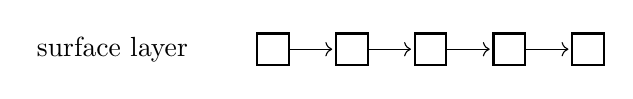
\begin{tikzpicture}[shorten >=1pt,->,draw=black!100,node distance = 1.3cm, auto]]
 	\def \startnode{1.5cm}
 	\tikzstyle{r-node}=[regular polygon sides=4,draw=black!100,thick,inner sep=0pt,minimum size=4mm]
 	\tikzstyle{annot} = [text width=3cm]
 	\node[annot] (surface-label) at (0cm,0cm) {surface layer};

 	\node[r-node] 	(r0)	at (\startnode,0cm)		{};
 	\node[r-node] 	(r1)	at (2.5cm, 0cm)		{};
 	\node[r-node] 	(r2)	at (3.5cm,0cm)	 	{};
 	\node[r-node] 	(r3)	at (4.5cm,0cm) 		{};
 	\node[r-node] 	(r4) 	at (5.5cm,0cm)   		{};
	
 	\path (r0)	edge	node	{}	(r1)
 		(r1)	edge	node	{}	(r2)
 		(r2)	edge	node	{}	(r3)
 		(r3)	edge	node	{}	(r4);
 \end{tikzpicture}
 \end{center}
 \caption{Sequential linear architecture.}
 %. Each representational unit depends on the preceding unit, and no unit exists outside of the surface layer.}
 \label{fig:seq-lin}
 \end{mdframed}
 \end{figure}
 
The first unsupervised morphological learners were SL algorithms. The earliest examples employed the 
Letter Successor/Predecessor Variety (LSV/LPV) measures \citep{harris:1955, harris:1967}. 
Both measures are intended to indicate likely affixes.
$\text{LSV}(x)$ is intended to find prefixes; given a string $x$ and corpus $W$, 
$\text{LSV}(x)$ returns the number of letter types that immediately follow $x$ whenever $x$ is word-initial in $W$.
Letter Predecessor Variety (LPV) is essentially the same measure, except that its function is to find suffixes,
and it works in the opposite direction:
It counts the grapheme types that immediately \emph{precede} $x$ whenever $x$ is \emph{word-final}.

By themselves, of course, LSV and LSP are merely counts; they must be ``unpacked" if they are to be used to discover legitimate morpheme boundaries.
There are a few different techniques for doing this
%using LSV/LSP to discover morpheme boundaries 
\citep[see][]{hammarstrom:2011}; one is the ``peak and plateau" technique. The following describes the use of peak and plateau with LSV:
\begin{itemize}
\item Given an $n$-length word $w$ whose graphemes are indexed from 0 to $n$, compute $\text{LSV}(w[0:i])$ for each $i$ in the range $[0, n)$.
%in the range $[0, n)$. 
\item Then, for each $i$ in $[0, n)$, insert a morpheme boundary after the substring $w[0:i]$ if and only if 
\begin{equation*}
\text{LSV}(w[0:i-1]) \le \text{LSV}(w[0:i]) \ge \text{LSV}(w[0:i+1]),
\end{equation*}
i.e., there is a local peak in the LSV sequence at index $i$.
\end{itemize}

It is not difficult to see the sequentiality and linearity of an LSV/LPV technique like peak and plateau.
% are not difficult to see.
Such a technique is sequential because its decision making process is shaped by the sequential order of graphemes.
An LSV technique, for example, must proceed left to right, one index at a time, because the LSV calculation at index $i$ depends on the preceding $i-1$ graphemes. Moreover, in peak and plateau, the question of whether or not to draw a morpheme boundary at index $i$ depends not only on the LSV at $i$, but also on the preceding and succeeding LSVs. LSV/LPV techniques are linear because they incorporate no hidden nodes and thus have no means of mediating associations between nonadjacent characters.
% process a string sequence of segmentation decisions proceeding either left to right or right to left, advancing one index at a time that is, at each $i$, the LSV count depends on the preceding $i-1$ graphemes. Notice also the technique's linearity:
%
%Notice the sequential nature of this technique: The algorithm makes a sequence of segmentation decisions proceeding left to right, advancing one index at a time. This left-to-right order is imposed by the definition of LSV; that is, at each $i$, the LSV count depends on the preceding $i-1$ graphemes. Notice also the technique's linearity:
%It has no hidden nodes and thus has no means of mediating associations between discontiguous substrings.
%; at each $i$, for instance, the algorithm can only ``see" the LSVs at $i-1$ and $i+1$
%starting at index 0. The definition of LSV makes  index $0$ to the final index$i$.
%A morphological classification decision is made at each index $i$ starting at the first index of the word in question and ending at the final index. 
%There is a necessary order to this chain of decisions because each decision must consider not only the LSV at $i$, but also the immediately preceding and succeeding LSVs
%First, the LSV count at each $i$ depends on the preceding $i-1$ graphemes. Then, a segmentation decision is made at each $i$
%each LSV calculation is determined solely by the immediately preceding string of graphemes. Note also its linearity: there is only a single layer of representation for both the grapheme sequence and the morphological analysis.

%The intuition behind the LSV/LPV method is essentially the same as that behind the entropy-based methods:
%in natural language processing:
%In fact, LSV generally increases/decreases as entropy increases/deceases:
The intuition behind the LSV/LPV method is that \emph{within} a morpheme, the identity of each letter depends on the letters that immediately precede or succeed it. But this is not the case \emph{between} morphemes. That is, the first letter of a morpheme is largely unpredictable given its preceding letters. Likewise, a morpheme's final letter is largely unpredictable given its succeeding letters. Thus, the number
 of possible letter types tends to increase sharply at the boundary between two morphemes.
%---and hence a larger LVP/LSV---at the boundary between two morphemes. 
%At any given point \emph{within} a morpheme, the next letter is fairly predictable, which generally coincides with a smaller number of succeeding letter types. But at the border between two morphemes, the next letter is much less predictable. This low predictability generally translates to a much larger set of options for the succeeding letter (i.e., a higher LSV). 
However, while morpheme boundaries generally coincide with high LVP/LSV counts, it is not necessarily true that a high LVP/LSV indicates a morpheme boundary.
%LSV is not always a reliable indicator of morpheme boundaries. 
\cite{hammarstrom:2011}, for example, provide LPV counts for the word \textit{disturbance}. 
The highest LPV count of 25 
%(i.e., 25 of the 26 possible letters in the English alphabet) 
occurs between \textit{disturbanc} and \textit{e}.
An LPV-based analysis would thus incorrectly identify \textit{e} as a suffix, a consequence of the ubiquity of \textit{e} as a stem-final letter in English spelling. 

%Goldsmith
Because of such problems, most linear sequential methods today have abandoned LSV/LPV, often in favor of frequency-based heuristics.
\cite{goldsmith:2001}, for example, uses a score based on pointwise mutual information (PMI) to approximate the likelihood that a given character $n$-gram $c_{1}c_{2}...c_{n}$ is a morpheme. 
%In particular, the PMI of the characters $c_{1}, c_{2}, ..., c_{n}$ is multiplied by the relative frequency of the $n$-gram $c_{1}c_{2}...c_{n}$. 
\cite{goldsmith:2001} obtains candidate suffixes (intended for further processing) by taking the $n$-grams that are ranked highest according to this score.  
%(i.e., the count of $c_{1}c_{2}...c_{n}$ divided by the total count of all $n$-grams). 

%Moon
\cite{moon-et-al:2009} apply tree data structures known as \textit{tries} to the task of finding stems and affixes, as have a number of other researchers \citep[e.g.,][]{schone-and-jurafsky:2000, monson:2004, argamon:2004}.
Tries are useful for learning concatenative morphology because they compactly store recurring character sequences.
Each node in a trie represents a certain prefix string (with the root node representing the empty string), 
and every path proceeding out from a node represents a possible succeeding character. 
Thus, even though tries are tree data structures, they process data in a sequential manner. 
They 
are linear
because they lack hidden nodes, and every path through a trie is deterministic. 
 \cite{moon-et-al:2009} depart from other trie-based methods in using document 
 boundaries to approximate semantic context. 
 This helps them weed out spurious analyses like the \textit{disturbanc}+\textit{e} 
 example above, but it does not change the fundamentally sequential and linear nature of their approach.
%\citep{goldsmith:2001} or trie-based affix-finding
%\citep{moon-et-al:2009}.
% , for example, uses a score based on pointwise mutual information
% (PMI) to approximate the likelihood that a given character $n$-gram
% %$c_{1}c_{2}...c_{n}$ 
% is a morphemic unit.
% In particular, the PMI of the characters $c_{1},
% c_{2}, ..., c_{n}$ is multiplied by the relative frequency of the
% $n$-gram $c_{1}c_{2}...c_{n}$. \cite{goldsmith:2001} obtains candidate
% suffixes by taking the $n$-grams that are ranked highest according to
% this score.
%(i.e., the count of $c_{1}c_{2}...c_{n}$ divided by the total count of all $n$-grams).  
%
%Moon
% \cite{moon-et-al:2009} apply tries to the task of finding stems and
% affixes, to store recurring character sequences.
%, as have a number of other researchers. 
% Tries are useful for learning concatenative morphology because they
% compactly store recurring character sequences.
%that are repeated a group of words. by sets of words beginning with the same character. 
% Each node in a trie represents a certain prefix string (with the root node representing the empty string), 
% and every path proceeding out from a node represents a possible succeeding character. 
% Thus, even though tries are tree data structures, 
%In all cases, the methods process data in a sequential manner and
%lack hidden nodes for representing morphological relationships.
% linearly, lacking hidden nodes.

% ; one of them is the ``peak and plateau" technique, which works as follows:
% \begin{itemize}
% \item Given an $n$-length word $w$ whose graphemes are indexed from 0 to $n$, compute $\text{LSV}(w[0:i])$ for each $i$ in the range $[0, n)$. \item Insert a morpheme boundary after the substring $w[0:i]$ if and only if $\text{LSV}(w[0:i-1]) \le \text{LSV}(w[0:i]) \ge \text{LSV}(w[0:i+1])$, i.e., there is a local peak in the LSV sequence at index $i$.
% \end{itemize}
% Notice the sequential nature of this technique: each LSV calculation is determined solely by the immediately preceding string of graphemes. Note also its linearity: there is only a single layer of representation for both the grapheme sequence and the morphological analysis.



% The intuition behind the LSV/LPV method is related to that behind the entropy-based methods in natural language processing:
% %In fact, LSV generally increases/decreases as entropy increases/deceases: 
% At any given point \emph{within} a morpheme, the next letter is fairly predictable, which generally coincides with a smaller number of succeeding letter types. But at the border between two morphemes, the next letter is much less predictable. This low predictability generally translates to a much larger set of options for the succeeding letter (i.e., a higher LSV). However, it out that LSV is not always a reliable indicator of morpheme boundaries. \cite{hammarstrom:2011}, for example, provide LPV counts for the word \textit{disturbance}. 
% The highest count (25) 
% %(i.e., 25 of the 26 possible letters in the English alphabet) 
% occurs between \textit{disturbanc} and \textit{e}, An LPV-based analysis would thus yield an incorrect result in this case, a consequence of the fact that \textit{e} is such a ubiquitous word-final letter in English spelling. 

%Goldsmith
% More recent linear sequential methods
% %have thus abandoned LSV/LPV, often in favor of
% use frequency-based heuristics.  \cite{goldsmith:2001}, for example,
% uses a score based on pointwise mutual information (PMI) to
% approximate the likelihood that a given character $n$-gram
% %$c_{1}c_{2}...c_{n}$ 
% is a morphemic unit.
% % In particular, the PMI of the characters $c_{1},
% % c_{2}, ..., c_{n}$ is multiplied by the relative frequency of the
% % $n$-gram $c_{1}c_{2}...c_{n}$. \cite{goldsmith:2001} obtains candidate
% % suffixes by taking the $n$-grams that are ranked highest according to
% % this score.
% %(i.e., the count of $c_{1}c_{2}...c_{n}$ divided by the total count of all $n$-grams).  
% %
% %Moon
% \cite{moon-et-al:2009} applies \textit{tries} to the task of finding stems and
% affixes, to store recurring character sequences in the search for recurring character sequences.
% % A number of other researchers have done the same.
% % Tries are useful for learning concatenative morphology because they
% % compactly store recurring character sequences.
% %that are repeated a group of words. by sets of words beginning with the same character. 
% % Each node in a trie represents a certain prefix string (with the root node representing the empty string), 
% % and every path proceeding out from a node represents a possible succeeding character. 
% % Thus, even though tries are tree data structures, 
% In all cases, the methods process data in a sequential manner and
% represent morphological relationships linearly, lacking hidden nodes.

% , and every path through a trie is deterministic.
% \cite{moon-et-al:2009} depart from other trie-based methods in using
% document boundaries to approximate semantic context.  This helps them
% weed out spurious analyses like the \textit{disturbanc}+\textit{e}
% example above, but it does not change the fundamentally sequential and
% linear nature of their approach.

\section{Non-sequential linear algorithms}
\label{subsec:nonseq-lin}
In the non-sequential linear (NSL) type of algorithm, shown in figure~\ref{fig:nonseq-lin}, the representational units are generally not raw characters, but rather \emph{features}, i.e., binary variables representing the presence or absence of particular properties.
%specifying whether or not a word has a certain property. 
Features in non-sequential algorithms need not correspond to continuous chunks of the original string; for example, features like the following are perfectly valid: ``\textit{t} precedes \textit{i} within $\delta-1$ characters" and ``\textit{t} precedes \textit{b} within $\delta-1$ characters," where the character pairs \emph{t..i} and \emph{t..b} are discontiguous as long as $\delta > 1$. Notice that such features cannot really be ordered; each is either \textsc{true} or \textsc{false} irrespective of order.
All non-sequential algorithms---of which NSL algorithms are a subcategory---view a given word's features as being unordered, that is, as being sequentially unrelated to each other. 
But while NSL algorithms are nonsequential, they are linear because they incorporate no hidden units. Thus, even though an NSL algorithm's features may refer to discontinuous subsequences of characters, they are nonetheless restricted to representing only properties that are overtly present in the surface layer of characters. 

One NSL example is the algorithm of \cite{poon-et-al:2009}, which uses log-linear models to induce morphological segmentations for Arabic and Hebrew. 
Log-linear models are inherently non-sequential because they treat all features as independent, estimating a global joint probability for the entire bag of features. 
%Sequential models, in contrast, estimate conditional probabilities based on sequential dependencies between features
The algorithm of \cite{poon-et-al:2009} in particular searches for the set of parameters $\theta$ that maximizes the joint probability of a corpus $W$ and a morphological segmentation $S$, i.e., $P(W,S| \theta) = P(W|S; \theta) \cdot P(S| \theta)$. The segmentation $S$ is encoded by a set of features.
%They generate candidate segmentations via Gibbs sampling. For each candidate, they extract a feature set

%Log-linear models are well-suited for large numbers of arbitrarily defined features. 
\cite{poon-et-al:2009} use two categories of features to encode a morphological segmentation: \textit{morpheme features} and \textit{morpheme context} features.
The former encode (potential) morpheme types and their frequencies, e.g., \texttt{vlAv:5} and \texttt{w:31}. The 
latter encode context types and their frequencies, where a \emph{context} consists of the $n$ characters preceding and succeeding a (potential) morpheme;
%the character bigrams to the left and right of a potential morpheme, 
e.g., the feature \texttt{\#w\_wn:12} would represent a context whose left side consists of \textit{w} preceded by the word boundary, whose right side is the bigram \textit{wn}, and whose frequency is 12. Importantly, these context features overlap. That is, in \texttt{\#w\_wn:12}, the \textit{w} and \textit{wn} are themselves morphemes whose contexts must be extracted.
This feature overlap is made possible by the non-sequentiality of log-linear models.
%is on the right, , respectively, and whose frequency of this particular context as 12.
%s that the left context is the character \textit{w} preceded by the word boundary, the right context is the character bigram \textit{wn}, and the frequency of this particular context is 12).
% and \textand the characters \textit{w} and \textit{n} are on the right potential morpheme\textit{w} on the left 
%and the characters \textit{w} and \textit{n} on the right).
%Note, however, that 

Note, however, that log-linear models can handle much more non-sequentiality than this. Indeed, because a log-linear model is inherently non-sequential, it can accommodate any sort of non-sequential feature. 
%one can incorporate into log-linear model.
%feature %or combination of feature types 
%in a log-linear model.  
One could, for example, incorporate
features representing discontiguous bigrams,
as already noted.
 One could also combine contiguous and discontiguous bigram features in the same feature set.
%for example, have features representing both contiguous and discontinous bigrams in the same feature set.
%However, one in principle could use any sort of feature in a log linear model, such as a feature type representing discontiguous bigrams, for example.
%Each feature represents the both corpus and the segmentation jointly, and a fully specified set of features thus represents an entire segmented corpus;
%but there is no limit on the variety or quantity of features one can incorporate into a log-linear model.
% Why is a log linear model non-sequential?
%Log-linear models are inherently non-sequential because they treat all features as independent, estimating a global joint probability for the entire bag of features. Sequential models, in contrast, estimate conditional probabilities based on sequential dependencies between features.
% Why is a log linear model non-sequential?
And yet it is not the nature of the features themselves that makes an algorithm non-sequential, but rather the lack of sequential relationships between features. The algorithm of \cite{poon-et-al:2009} is non-sequential because it does not process features in a particular order.
% Why is Poon et al's algorithm linear?
It is, however, linear because it incorporates no hidden units to mediate associations between features.

%\cite{poon-et-al:2009} incorporate no latent variables, however. 
%Their representation of morphological structure makes reference only to the the surface layer of graphemes. Their morpheme features are limited to  contiguous grapheme sequences, 
%and their morpheme context features encode only extreme left and right contexts, 
%thus assuming no internal boundaries (i.e., no morpheme interruptions).
%%They generate candidate segmentations via Gibbs sampling, but, for an $n$-length word, they consider 
%Because it only acknowledges the surface layer of text, the algorithm of \cite{poon-et-al:2009} can only isolate stems and affixes, not the discontiguous roots and patterns of Arabic and Hebrew.

%\paragraph{Non-sequential linear algorithms}
%\label{subsec:nonseq-lin}
%
%Like SL algorithms, \textbf{non-sequential linear} (NSL) algorithms consist only of surface units, having no hidden layer, hence their linearity. NSL algorithms are different in that there are no dependencies between representational units. Each unit is independent of other units, hence their \textit{non-sequential} characterization.
%%They consist only of surface units, hence their linearity. What sets NSL algorithms apart is the lack of dependencies between these units, h
%%illustrated in figure~\ref{fig:nonseq-lin}, 
%%there are no dependencies between representational units, but also no
%%hidden units.
%%; i.e., all representational units reside in the surface layer.  
%As one example, \cite{poon-et-al:2009} use log-linear models to induce
%morphological segmentations for Arabic and Hebrew. 
%% Their algorithm
%% searches for the set of parameters $\theta$ that maximizes the joint
%% probability of a corpus $W$ and a segmentation $S$ (i.e., $P(W,S|
%% \theta)$).
%% = P(W|S; \theta) \cdot P(S| \theta)$.
%%They generate candidate segmentations via Gibbs sampling. For each candidate, they extract a feature set
%% Log-linear models are well-suited for large numbers of arbitrarily
%% defined features.
%% \cite{poon-et-al:2009} use morpheme features and morpheme context
%% features.  The former category specifies a morpheme type and its
%% frequency, e.g., \texttt{vlav:1} and \texttt{w:2}.  The latter
%% category indicates the character bigrams to the left and right of a
%% given morpheme, e.g., \texttt{\#w\_wn:1} (a word boundary followed by
%% the character \textit{w} on the left and the characters \textit{w} and
%% \textit{n} on the right).  Note, however, that one could use any type
%% of feature or combination of feature types with a log-linear
%% model. One could, for example, have features representing both
%% contiguous and discontinues bigrams in the same feature set.
%%
%%However, one in principle could use any sort of feature in a log linear model, such as a feature type representing discontiguous bigrams, for example.
%%Each feature represents the both corpus and the segmentation jointly, and a fully specified set of features thus represents an entire segmented corpus;
%%but there is no limit on the variety or quantity of features one can incorporate into a log-linear model.
%% Why is a log linear model non-sequential?
%Log-linear models are non-sequential because they treat all features
%as independent, estimating a global joint probability.
%%for the entire bag of features.
%% Sequential models, in contrast, estimate conditional probabilities
%% based on sequential dependencies between features.
%% Why is Poon et al's algorithm linear?
%% \cite{poon-et-al:2009} incorporate no latent variables,
%% %, however, 
%% %Their representation of morphological structure makes 
%% referencing only the the surface layer of graphemes.
%% Their morpheme
%% features are limited to contiguous grapheme sequences, and their
%% morpheme context features encode only extreme left and right contexts,
%% thus assuming no internal boundaries (i.e., no morpheme
%% interruptions).  
%Even though such a log-linear model allows for any type of feature,
%including both contiguous and discontiguous $n$-grams,
%%They generate candidate segmentations via Gibbs sampling, but, for an $n$-length word, they consider  
%the algorithm ultimately can only isolate stems and affixes, because
%it only acknowledges the surface layer of text.
%%, and not discontiguous roots and patterns.
%% of Arabic and Hebrew.

 \begin{figure}[t]
\begin{mdframed}
 %\begin{minipage}{.3\textwidth}
 \begin{center}
 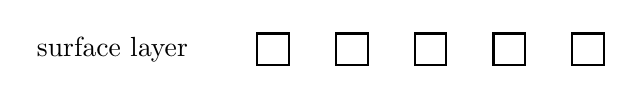
\begin{tikzpicture}[shorten >=1pt,->,draw=black!100]
 	\def \startnode{1.5cm}
 %	\def\secondrow{1.0cm}
 	\tikzstyle{r-node}=[regular polygon sides=4,draw=black!100,thick,inner sep=0pt,minimum size=4mm]
 	\tikzstyle{annot} = [text width=3cm]
 	% labels
 	\node[annot] (surface-label) at (0cm,0cm) {surface layer};
 %	\node[annot] (r-label) at (0, \secondrow) {prediction vector};
 %	\node[annot] (d-label) (0, 0) {observed data vector};
	
 	% surface layer
 	\node[r-node] 	(r0)	at (\startnode,0cm)		{};
 	\node[r-node] 	(r1)	at (2.5cm, 0cm)		{};
 	\node[r-node] 	(r2)	at (3.5cm,0cm)	 	{};
 	\node[r-node] 	(r3)	at (4.5cm,0cm) 		{};
 	\node[r-node] 	(r4) 	at (5.5cm,0cm)   		{};
	
 %	\path (r0)	edge	node	{}	(r1)
 %		(r1)	edge	node	{}	(r2)
 %		(r2)	edge	node	{}	(r3)
 %		(r3)	edge	node	{}	(r4);
 \end{tikzpicture}
 \end{center}
 \caption{Non-sequential linear architecture}
 
 %. No dependencies exist between representational units, and no unit exists outside of the surface layer.}
 \label{fig:nonseq-lin}
  \end{mdframed}
 \end{figure}

% \cite{poon-et-al:2009} use morpheme features and morpheme context
% features.  The former category specifies a morpheme type and its
% frequency, e.g., \texttt{vlav:1} and \texttt{w:2}.  The latter
% category indicates the character bigrams to the left and right of a
% given morpheme, e.g., \texttt{\#w\_wn:1} (a word boundary followed by
% the character \textit{w} on the left and the characters \textit{w} and
% \textit{n} on the right).  Note, however, that one could use any type
% of feature or combination of feature types with a log-linear
% model. One could, for example, have features representing both
% contiguous and discontinues bigrams in the same feature set.


\section{Sequential nonlinear algorithms}
\label{subsec:seq-nonlin}
% First, what sort of algorithms are sequential nonlinear?
The sequential nonlinear (SNL) type of algorithm is illustrated in figure~\ref{fig:seq-nonlin}. 
Note in particular the addition of a hidden layer, whose units (the circular nodes)
represent the underlying sources of the surface data's implicit structure.
%account for the surface %the surface units and thus take responsibility for the regularities ac
%for 
%algorithms differ from sequential linear ones in that 
%they add a layer of hidden units for 
%encoding 
%take responsibility for generating the structure implicit
%the regularities %, i.e., the implicit structure, 
%in the surface layer and thus the
%data.
%These hidden units can be viewed as causing or generating the surface data.
SNL algorithms are nonlinear because they incorporate a hidden layer.
However, they are sequential because the hidden layer in an SNL algorithm is sequential; i.e., its component hidden units
%hidden units
are sequentially ordered.
Since the surface units depend on the hidden units, the hidden layer imposes its sequential order on the surface layer. 
%they have a certain each hidden unit depends on its predecessor hidden unit(s). 
% I need to say what the nonlinear aspect brings to the table. If being nonlinear is beneficial, sequential nonlinear algorithms should be better than sequential linear ones. So what do sequential nonlinear algorithms have that sequential linear algorithms don't? How does being nonlinear help them?
% First, what sort of algorithms are sequential nonlinear?

%Sequential nonlinear (SNL) algorithms
%%, illustrated in figure~\ref{fig:seq-nonlin}, 
%differ from sequential
%linear ones by adding a layer of hidden units for encoding the
%structure of the surface layer.
%This makes them nonlinear. 
% They are still sequential, however, in that there are sequential
% dependencies within the hidden layer.
%; i.e., each hidden unit depends on its predecessor hidden unit(s).
%The prototypical example of a sequential nonlinear model is the Hidden
%Markov Model (HMM).  \cite{creutz-and-lagus:2005,
%  creutz-and-lagus:2007} employ an HMM to induce a morphological
%lexicon.
The prototypical SNL model is the Hidden Markov Model (HMM). 
\cite{creutz-and-lagus:2005, creutz-and-lagus:2007} employ an HMM to induce a morphological lexicon, i.e., a list of morpheme-like segments they call \textit{morphs}. 
%, i.e., a list of morpheme-like segments.
%that they call \textit{morphs}.
%sorted in order of increasing morph length. 
%They take a maximum a posteriori (MAP) approach.
Their algorithm seeks to find the lexicon such that $P(lexicon|corpus)$ is maximized. Due to Bayes' theorem, this equates to finding the lexicon that maximizes $P(corpus|lexicon) \cdot P(lexicon)$. The probability $P(corpus|lexicon)$ is computed by an HMM. Each unit in this HMM's hidden layer can take on five possible values: \textit{prefix}, \textit{stem}, \textit{suffix}, \textit{word boundary}, and \textit{non-morpheme}. 
Note how the first four relate sequentially to each other: prefixes must precede stems, stems must precede suffixes, and so on.
%The observation sequence is a segmentation hypothesis, i.e., a candidate segmentation of the corpus into morphs. 
%Candidate segmentations are generated independently of the HMM, as are the transition and emission probabilities. 
%The HMM's role to find likely hidden state sequence, which is computed by the Viterbi algorithm, along with the probability $P(corpus|lexicon)$. 
The hidden layer in this case serves to facilitate the search for the optimal lexicon 
(i.e., segmentation) by providing a means of abstracting away from the literal surface characters.

%The HMM's role is to evaluate each candidate morph sequence. 
% took out the "h"
 \begin{figure}[t]
 \begin{mdframed}
 %\begin{minipage}{.3\textwidth}
 \begin{center}
 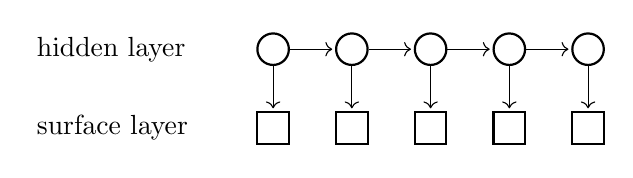
\begin{tikzpicture}[shorten >=1pt,->,draw=black!100]
 	\def \rowtwoht{1.0cm}
 	\def \rowoneht{0.0cm}
 	\tikzstyle{m-node}=[circle,draw=black!100,thick,inner sep=0pt,minimum size=4mm]
 	\tikzstyle{r-node}=[regular polygon sides=4,draw=black!100,thick,inner sep=0pt,minimum size=4mm]
 	\tikzstyle{annot} = [text width=3cm]
 	% labels
 	\node[annot] (hidden-label) at (0cm,\rowtwoht) {hidden layer};
 	\node[annot] (surface-label) at (0cm,\rowoneht) {surface layer};

 %	\node[annot] (d-label) (0, 0) {observed data vector};
	
 	% hidden layer
 	\node[m-node] 	(m0)	at (1.5cm,\rowtwoht)		{};
 	\node[m-node] 	(m1)	at (2.5cm,\rowtwoht)		{};
 	\node[m-node] 	(m2)	at (3.5cm,\rowtwoht)	 	{};
 	\node[m-node] 	(m3)	at (4.5cm,\rowtwoht) 		{};
 	\node[m-node] 	(m4) 	at (5.5cm,\rowtwoht)   		{};
	
 	% surface layer
 	\node[r-node] 	(r0)	at (1.5cm,\rowoneht)		{};
 	\node[r-node] 	(r1)	at (2.5cm,\rowoneht)		{};
 	\node[r-node] 	(r2)	at (3.5cm,\rowoneht)	 	{};
 	\node[r-node] 	(r3)	at (4.5cm,\rowoneht) 		{};
 	\node[r-node] 	(r4) 	at (5.5cm,\rowoneht)   		{};
	
 	\path (m0)	edge	node	{}	(m1)
 		(m1)	edge	node	{}	(m2)
 		(m2)	edge	node	{}	(m3)
 		(m3)	edge	node	{}	(m4);
		
 	\path (m0)	edge	node	{}	(r0)
 		(m1)	edge	node	{}	(r1)
 		(m2)	edge	node	{}	(r2)
 		(m3)	edge	node	{}	(r3)
 		(m4)	edge	node	{}	(r4);		
 \end{tikzpicture}
 \end{center}
 \caption{Sequential nonlinear architecture}
 \label{fig:seq-nonlin}
 \end{mdframed}	
 \end{figure}

\section{Non-sequential nonlinear algorithms}
\label{subsec:nonseq-nonlin}
% Intro
 Like sequential nonlinear (SNL) algorithms, \textit{non}-sequential
 nonlinear (NSNL) algorithms incorporate a hidden layer whose units generate the observed
 units of the surface layer.
The difference is that the hidden layer in an NSNL algorithm is \emph{non-sequential}; 
i.e., the algorithm computes the values of all hidden units in parallel rather than in a sequence.
The surface layer in a NSNL algorithm is also non-sequential.
 %dependencies.
 Thus, every unit---whether hidden or surface---is entirely independent
 within its own layer. Figure~\ref{fig:nonseq-nonlin} illustrates the NSNL framework; notice that no two nodes with the same layer are connected by an arc.
This intra-layer independence allows a hidden unit to associate with
any combination of surface units, whether contiguous or discontiguous

 \begin{figure}[t]
 \begin{mdframed}	
 %\begin{minipage}{.3\textwidth}
 \begin{center}
 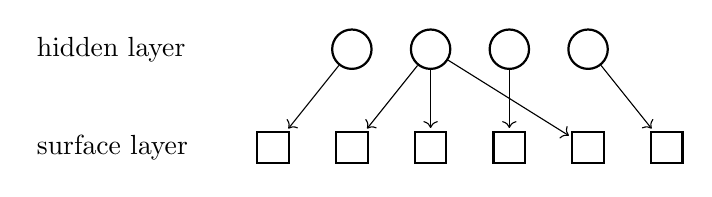
\begin{tikzpicture}[shorten >=1pt,->,draw=black!100] %,scale=.95]
 	\def \rowtwoht{1.25cm}
 	\def \rowoneht{0.0cm}
 	\tikzstyle{m-node}=[circle,draw=black!100,thick,inner sep=0pt,minimum size=5mm]
 	\tikzstyle{r-node}=[regular polygon sides=4,draw=black!100,thick,inner sep=0pt,minimum size=4mm]
 	\tikzstyle{annot} = [text width=3cm]
 	% labels
 	\node[annot] (hidden-label) at (0cm,\rowtwoht) {hidden layer};
 	\node[annot] (surface-label) at (0cm,\rowoneht) {surface layer};

 %	\node[annot] (d-label) (0, 0) {observed data vector};
	
 	% hidden layer
 	\node[m-node] 	(m0)	at (2.5cm,\rowtwoht)		{};
 	\node[m-node] 	(m1)	at (3.5cm,\rowtwoht)		{};
 	\node[m-node] 	(m2)	at (4.5cm,\rowtwoht)	 	{};
 	\node[m-node] 	(m3)	at (5.5cm,\rowtwoht) 		{};
	
 	% surface layer
 	\node[r-node] 	(r0)	at (1.5cm,\rowoneht)		{};
 	\node[r-node] 	(r1)	at (2.5cm,\rowoneht)		{};
 	\node[r-node] 	(r2)	at (3.5cm,\rowoneht)	 	{};
 	\node[r-node] 	(r3)	at (4.5cm,\rowoneht) 		{};
 	\node[r-node] 	(r4) 	at (5.5cm,\rowoneht)   		{};
 	\node[r-node] 	(r5) 	at (6.5cm,\rowoneht)   		{};
	
 	\path (m0)	edge	node	{}	(r0)
 		(m1)	edge	node	{}	(r1)
 		(m2)	edge	node	{}	(r3)
 		(m1)	edge	node	{}	(r2)
 		(m1)	edge	node	{}	(r4)
 		(m3)	edge	node	{}	(r5);
		
 \end{tikzpicture}
 \end{center}
 \caption{Non-sequential nonlinear architecture}
 \label{fig:nonseq-nonlin}
 \end{mdframed}	
 \end{figure}

The NSNL type can take many forms. 
\cite{baroni-et-al:2002}, for example, detect implicit causal units by computing 
the Levenshtein alignments for pairs of words. 
The Levenshtein algorithm finds the minimum number of edit operations 
(typically allowing substitutions, deletions, and insertions) required to change 
a \textit{source} word into a \textit{target} word.
An alignment of the source and target characters is obtained as a by-product 
of computing the edit operations.
characters of the source with those of the target word. 
From the alignment, one can extract the (not necessarily contiguous) 
subsequence held in common by the two words.
%One might view the common subsequence as suggesting a sin
Thus, one may view the alignment as suggesting a single causal unit behind 
both occurrences of the subsequence, i.e., as a kind of implicit hidden unit, 
as it were.
For example, the alignment in figure~\ref{fig:lev-align} implies a single cause 
behind both occurrences of the subsequence \textit{dbr}.
Of course, a common subsequence does not necessarily indicate a 
morphological relationship; 
consider, for instance, the English pair \textit{pork}/\textit{park}. 
To avoid finding spurious relationships, 
\cite{baroni-et-al:2002} compute a semantic similarity score based on 
mutual information, 
combining it with an orthographic similarity score based on minimum 
edit distance (\text{ED}).

 \begin{figure}[t]
 \begin{mdframed}
  \vspace{10pt}
 %\begin{minipage}{.3\textwidth}
 \begin{center}
 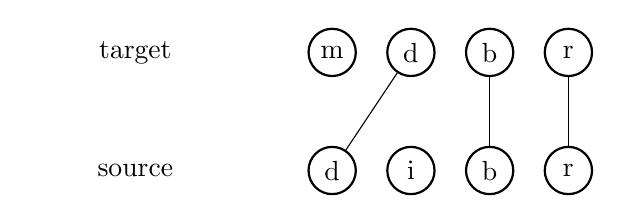
\begin{tikzpicture}[draw=black!100]
 	%[shorten >=1pt,->,draw=black!100]
 	\def \rowtwoht{1.5cm}
 	\def \rowoneht{0.0cm}
 	\tikzstyle{m-node}=[circle,draw=black!100,thick,inner sep=0pt,minimum size=6mm]
 	\tikzstyle{r-node}=[circle,draw=black!100,thick,inner sep=0pt,minimum size=6mm]
 	\tikzstyle{annot} = [text width=2.5cm, text centered]
 	% labels
 	\node[annot] (hidden-label) at (0cm,\rowtwoht) {target};
 	\node[annot] (surface-label) at (0cm,\rowoneht) {source};

 %	\node[annot] (d-label) (0, 0) {observed data vector};
	
 	% hidden layer
 	\node[m-node] 	(m0)	at (2.5cm,\rowtwoht)		{m};
 	\node[m-node] 	(m1)	at (3.5cm,\rowtwoht)		{d};
 	\node[m-node] 	(m2)	at (4.5cm,\rowtwoht)	 	{b};
 	\node[m-node] 	(m3)	at (5.5cm,\rowtwoht) 		{r};
	
 	% surface layer
 	\node[r-node] 	(r0)	at (2.5cm,\rowoneht)		{d};
 	\node[r-node] 	(r1)	at (3.5cm,\rowoneht)		{i};
 	\node[r-node] 	(r2)	at (4.5cm,\rowoneht)	 	{b};
 	\node[r-node] 	(r3)	at (5.5cm,\rowoneht) 		{r};
 	%\node[r-node] 	(r4) 	at (6.5cm,\rowoneht)   		{};
 	%\node[r-node] 	(r5) 	at (7.5cm,\rowoneht)   		{};
	
 	\path (m1)	edge	node	{}	(r0)
 		(m2)	edge	node	{}	(r2)
 		(m3)	edge	node	{}	(r3);
 %		(m3)	edge	node	{}	(r3)
 %		(m1)	edge	node	{}	(r4)
 %		(m3)	edge	node	{}	(r5);
		
 \end{tikzpicture}
 \end{center}
 \caption{The minimum-edit-distance alignment for the Hebrew words \textit{dibr} `he spoke' and \textit{mdbr} `he is speaking'. The discontiguous root \textit{d.b.r } is discovered by aligning \textit{dibr} with \textit{mdbr} and extracting the common subsequence.}
 \label{fig:lev-align}
 \end{mdframed}
 \end{figure}


Other authors simulate a nonlinear, multi-tier representation by 
separating the 
learning process into two or more phases.
The first phase classifies individual literal characters into abstract categories 
that are then 
used by a second phase (and perhaps subsequent phases) to perform other 
aspects of the analysis.
Multiple phases occurring at different times can thus replicate the effects 
of multiple simultaneous levels of representation.
This is the approach taken by \citet{rodrigues-and-cavar:2005} to induce 
the non-concatenative morphology of Arabic. 
%Following the statistical constraint-based method of \cite{elghamry:2005}, 
Their first phase identifies root radicals according to the statistical 
constraint-based method of \citet{elghamry:2005}. 
For each word in their corpus, 
they generate a set of candidate triliteral roots according to 
constraints derived from the tendencies of Arabic roots as observed in corpora. 
In particular, any 3-length subsequence is admitted into the candidate set 
if and only if it satisfies both of the following:
\begin{enumerate} 
\item No two consecutive radicals may be separated by more than two characters.
\item No more than four characters intervene between the first and third radicals.
\end{enumerate}
Then, a statistical score is computed for each candidate, and the one with the highest score is selected as the root.
Once the roots---and thus the stems---have been isolated by the first phase, the second phase identifies the concatenative affixes through a separate methodology.

% Goldsmith and Xanthos
An alternative first-phase strategy can be found in \citet{goldsmith-and-xanthos:2009}, 
who present methods for
partitioning a phonemic inventory into a class of consonants and a class of vowels. 
Their paper does not go into automatic morphological analysis, but it is not difficult to see how C and V classes could be useful to a multi-phase morphological analyzer.
The first phase would partition the phonemic inventory and, for each word, label each phoneme/grapheme as either a consonant or vowel, thus creating a sort of CV skeleton similar to the segmental tier of autosegmental phonology.
Subsequent phases would then use these CV skeletons to isolate roots, patterns, and other morphemes.

While the NSNL approaches described in this section provide a means for detecting discontiguous morphemes, they are not without their weaknesses.
The algorithm of \citet{baroni-et-al:2002} must filter out a large proportion of its input corpus, accepting only the words with relative frequencies of less than 0.01 percent; which are presumed to be content words.
It also relies on arbitrary thresholds; e.g., the threshold for the orthographic similarity measure (defined as $1 - \text{NED}$,  i.e., `$1$ minus the \emph{normalized} minimum edit distance') is set at 0.5, although there is no obvious reason why this should be so.
Note also that behind this threshold is the assumption that morphologically related words share at least half of their characters, which is not necessarily true. Such an assumption would be especially problematic for highly agglutinative languages, 
in which it is not uncommon for a stem to comprise a minority of a word's characters.
Moreover, the Levenshtein edit-distance approach is only capable of comparing words pairwise, which only allows morphological relationships to be expressed on a pairwise basis. This is a consequence of the lack of an explicitly encoded hidden causal layer; an explicit (as opposed to implicit) hidden layer could easily mediate multi-way associations among surface layer components.                                   

% Rodrigues and Cavar
%% Only tri-literal roots
Moreover, \citet{rodrigues-and-cavar:2005}, following \citet{elghamry:2005}, limit their algorithm's search to triliteral roots in order to reduce the problem's complexity, even though quadriliteral roots are not uncommon in Hebrew or Arabic.
%% Reasonable constraints, but constraints nonetheless. A truly general algorithm wouldn't need constraints. 
And while their two constraints on candidate-root generation are quite reasonable, these constraints are particular to the case of Semitic morphology, and thus they would not be required by a truly general algorithm.

Finally, none of the works discussed in this section represents both the hidden layer and surface layer simultaneously in a single, straightforward model. In contrast, the Multiple Cause Mixture Model (MCMM) \citep{saund:94} is an NSNL algorithm that explicitly represents both surface and hidden nodes in a single graphical model. The MCMM is the focus of the next section.

\section{Conclusion}
In sum, both \emph{nonlinearity} and \emph{nonsequentiality} must be present in an algorithm if it is to be handle nonconcatenative morphology. As we have seen through the examples in this chapter, it is not sufficient to have just one of these properties without the other. In the next chapter, we will glean deeper insight into nonlinearity and nonsequentiality by relating them to the mathematical properties of \emph{bipartite} graphs. 
\chapter{Graph-Theoretic Foundation}
\label{ch:graph}
\section{Introduction}
The purpose of this chapter is to motivate the use of the \ac{MCMM} as Multimorph's learning framework. The key concept in this chapter will be the \emph{bipartite} graph, a type of graph so named because its nodes can be partitioned into two subsets according to criteria which we shall discuss below. This chapter will maintain that bipartite graphs have properties that are essential to the tasks of modeling and learning non-concatenative morphology.
% a type of graph with two sets of nodes such that only nodes of different sets are connected. Within each set, there are no connections. This intra-layer independence engenders some important properties, as we shall see.
We shall begin in section~\ref{sec:bipartite} by introducing the mathematical concept of the \emph{bipartite graph}, placing particular importance on the properties that make this type of graph naturally conducive to modeling non-concatenative morphology. %We shall demonstrate that bipartite graphs are essential for the modeling of nonconcatenative morphology (and thus morphology in general). 

In section~{sec:autoseg-bipart} we shall take a fresh look at McCarthy's autosegmental framework for morphology \citep{mccarthy:1981} in light of the properties of the bipartite graph. We shall thus see that not only is McCarthy's framework itself bipartite graph, but that the properties of bipartite graphs are essential for the modeling of non-concatenative morphology.
% naturally well-suited to modeling non-concatenative morphology. and more than that, we will argue that bipartite graphs are general that ultimately derive from these properties two necessary conditions that morphological models must satisfy in order to be capable of modeling bipartite graphs two criteria that a morphological model must satisfy We will see that McCarthy's framework is itself a bipartite graph. and re
Finally, in section~\ref{mcmm-bipart}, we point out that an \ac{MCMM} is a bipartite graph, and that, consequently, it is compatible so to  speak with autosegmental morphology. In other words, an MCMM can serve as a
a computational ``wrapper," so to speak, for McCarthy's autosegmental theory, a means whereby it can be specially packaged for use in a machine learning system. 
 
%itself has a bipartite architecture, which is to say that it can be represented as and thought of as a bipartite graph without information loss.  essentially bipartite in its architecture, and that it ; we will see that the autosegmental framework is essentially a bipartite graph. We shall then observe in section~\ref{sec:mcmm-bipart} that an \ac{MCMM} is itself a bipartite graph, and that autosegmental morphology and \ac{MCMM}s have the same graphical properties. From this point, the conclusion follows that an From a theoretical perspective, therefore, it is a sound choice to use the \ac{MCMM} as a computational``wrapper," as it were, for McCarthy's theoretical autosegmental framework, to package for it for use a machine learning system. 
%The argumentation in this chapter will proceed as follows: 
%\begin{enumerate}
%\item We shall first demonstrate that the autosegmental morphological framework of \cite{mccarthy:1981} is, in its essence, a bipartite graph.
%\item We shall then observe that an \ac{MCMM} is quite clearly a bipartite graph. 
%\item From these two points, it follows that autosegmental morphology and \cm
%\end{enumerate}

%We shall first show that McCarthy's autosegmental morphological framework of \cite{mccarthy:1981} is a bipartite graph. We we shall show that an MCMM is a bipartite graph. And connecting the latter point to the former, %the latter point to the former, 
%we shall conclude that because the MCMM and McCarthy's autosegmental formalism 
%are both bipartite graphs, the MCMM is a very appropriate learning framework for 
%modeling autosegmental morphology and thus for learning nonconcatenative 
%morphology. The \ac{MCMM}, therefore, is well-suited to serve as a computational implementation of autosegmental morphology. %mathematically, and in particular, graph-theoretically. , we shall introduce the \emph{multipartite graphs}, 
%particularly \emph{bipartite graphs}, as well as discuss their relationship to autosegmental morphology, and hence their significance to the problem of
%learning non-concatenative morphology.   
%relevance to the problem of leand their relationship 
%to autosegmental morphology.
% which are a subset, i.e., special case, of multipartite graphs. 
\section{Bipartite Graphs}\label{sec:bipartite}
A \emph{multipartite} graph is a graph 
whose nodes can be partitioned into $N$ disjoint sets of 
\emph{mutually nonadjacent} nodes, i.e., $N$ sets such that no two
nodes within the \emph{same} set are connected by an edge. A bipartite graph
is simply multipartite graph such that $N = 2$. Thus, a bipartite graph is defined 
as in \ref{ex:bipartite}: 
%graph that satisfies the following: i.e., it has two partitions of nodes  That is, a graph is \textbf{bipartite} if it satisfies the following
%criteria in \ref{ex:bipartite}.
%\begin{definition} A graph is \textbf{bipartite} if it satisfies the following criteria:
%\begin{enumerate}
%\item The graph's nodes are separated into two disjoint sets (or partitions).
%\item Within each partition, all nodes are independent, i.e., mutually nonadjacent.
%\end{enumerate}
\begin{exe} \label{ex:bipartite} \ex A \textbf{bipartite} graph is a graph in which:\begin{xlist} 
	\ex %{\textsc{Nonlinearity}}.  %A model is \emph{nonlinear} 
	the nodes divided into two disjoint sets, or partitions. \label{ex:bipartite1} %separated into two disjoint sets, or partitions. %eparately for m  as being separate from (or outside of) the the phonological (or segmental) tier.  % is a property wherein morphs are represented as being separate from the segmental tier.
	\ex %Within each partition, nodes are mutually non-adjacent. % ; 
	Two nodes are members of the same partition if and only if 
	they are \emph{not} connected by an edge.
	\label{ex:bipartite2}
	\end{xlist}
\end{exe}
%\end{definition}
(i.e., non-adjacent). Conversely, 
	if two nodes \emph{are} connected (or adjacent), they necessarily belong to different sets. 
	\emph{This means that \textbf{within} each or partition, all nodes are independent 
	(i.e., not connected).}
These two criteria are equivalent to the properties of nonlinearity and 
nonsequentiality, respectively, first defined in chapter~\ref{ch:intro}.

\section{Autosegmental Morphology is Bipartite}\label{sec:autoseg-bipart}
The central aspect of autosegmental theory 
is its \emph{multi-linear} architecture, i.e., its use of a 
\emph{segmental tier} along with many \emph{autosegmental tiers} to 
account for the surface forms of words\ cite{mccarthy:1981}. The segmental tier is home to the sequence of consonants and vowels that define the linear arrangement of phonological features. Each autosegmental tier is home to a morph. Each morph, therefore, occupies its own distinct plane and is thus external to the segmental tier. The separation of morphs from the segmental tier allows a given morph to connect to nonadjacent phonological segments, as illustrated in figure~\ref{subfig:multilinear}. %as well as from each other gives rise to a multi-linear architecture. 
The multi-linear architecture of autosegmental theory thus provides a means of
dealing with nonconcatenative morphology. 

One can see this plainly by comparing figures~\ref{subfig:multilinear} and \ref{subfig:linear}. Each shows an attempt to analyze the word \emph{hizkir} `he reminded', in which the root \textit{z-k-r} (morph $\mu_3$) is interrupted by the /i/ of morph $\mu_2$ and is thus a discontinuous, or non-concatenative morph. Figure~\ref{subfig:multilinear} is a multilinear autosegmental approach (or nonlinear nonsequential type of model described in chapter~\ref{ch:LitReview}), whereas figure~\ref{subfig:linear} is a linear approach. The multilinear approach is able to recognize the root \textit{z-k-r} as a coherent morph despite its discontinuity. The linear approach, by contrast, has no way to group the \textit{r} with the \textit{z} and {k}.

In figure~\ref{subfig:multilinear}, we see at work the properties \emph{nonlinearity} and \emph{nonsequentiality}, first defined in chapter~\ref{ch:lit-review}.
Let us restate these properties here as (\ref{ex:criteria1-again}) and (\ref{ex:criteria2-again}).
\begin{exe} \label{ex:criteria-again} \ex \begin{xlist}
	\ex {\textsc{Nonlinearity}}.  %A model is \emph{nonlinear} 
	Morphs must be separate from the phonological tier. \label{ex:criteria1-again}
%	Morphs must be represented separately 
%	from the surface (or phonological) tier, i.e., as residing on tiers distinct from 
%	the phonological tier. \label{ex:criteria1-again}%eparately for m  as being separate from (or outside of) the the phonological (or segmental) tier.  % is a property wherein morphs are represented as being separate from the segmental tier.
	\ex {\textsc{Nonsequentiality}}.
	Each morph tier must be orthogonal to all other morph tiers. \label{ex:criteria2-again}
	%Each morph tier is required to be orthogonal to all other morph tiers. \label{ex:criteria2-again}
	\end{xlist}
\end{exe}

%	\begin{definition}\label{def:nl}{\textsc{Nonlinearity}}: %A model is \emph{nonlinear} 
%	Morphs must be separate from the phonological tier. \end{definition}
%	%Morphs, i.e., units of morphological structure, must be separate from the surface (or phonological) tier. \end{definition} %, i.e., as residing on tiers distinct from the phonological tier. %eparately for m  as being separate from (or outside of) the the phonological (or segmental) tier.  % is a property wherein morphs are represented as being separate from the segmental tier.
%	\begin{definition}\label{def:ns}{\textsc{Nonsequentiality}}: %is a property such that each morph tier (or node) is orthogonal to all other morph tiers.
%	%---i.e., independent of---all other morph tiers. 
%	Each morph tier must be orthogonal to all other morph tiers.
%	\end{definition}
%\begin{proposition}\label{prop:nlns}
%A model of morphology can handle nonconcatenative morphology if and only if it satisfies both \textbf{nonlinearity} and \textbf{nonsequentiality}. %  the modeling of nonconcatenative morphology.}
%\end{proposition}
%\pex~ Two essential properties  %\ex \label{ex:properties}\begin{xlist}
%	\a {\textsc{Nonlinearity}}: Morphemes are represented as being separate from the segmental tier.
%	\a {\textsc{Nonsequentiality}}: Each morpheme tier (or node) is orthogonal to---i.e., independent of---all other morpheme tiers.
%\xe
% \ex this is one 
%\marginpar{or multilinear}

%and comprises one or more (not necessarily contiguous) feature bundles. Each feature bundle can associate with any phonological segment in the \emph{segmental tier} as long as the association lines of  
%In chapter~\ref{ch-Intro}, I stated that 
%Recall that one of this dissertation's primary objectives is to implement autosegmental morphology computationally, so that it might equip an unsupervised machine learning system to learn non-concatenative morphology, 
There is a clear correspondence between these two properties  %(\ref{ex:criteria1-again}) (\ref{ex:criteria2-again})  
and the two components of the definition of \emph{bipartite} in (\ref{ex:criteria-again}).
The reason for this correspondence is that the autosegmental framework is essentially a bipartite graph. 
We can make this clearer simply be rearranging the morph nodes $\mu_1$, $\mu_2$, and $\mu_3$. That is, can simply move up $\mu_2$ so that it is situated between $\mu_1$ and $\mu_3$, i.e., so that all three morphs are lined up in a row. We can then regard this row (or vector) of morphs as one of the partitions in a bipartite graph. The segmental tier would constitute the other partition. And since all components in a vector are orthogonal to one another, the morph in a vector of morphs can still be regarded as residing on different tiers. %This would not effect the indpendence of th mo
%in order to enable this system
% Explored in linguistic theory and computationally with hand-written grammars ...
%to learn nonconcatenative morphology without supervision. 
%in a machine learning system capable of learning nonconcatenative morphology without supervision.
%During the course of development, I will explore different options for system components, e,g., the set of features,
%in order to arrive at the configuration that gives the best result for learning autosegmental morphology.  

%0. Already accepted as fact/Already proposed/hypothosized. Isolate the aspect(s) of AT that are responsible 
%for its ability to deal with nonconcatenative morphology.
%\cite{mccarthy:1981} has shown that it is the multi-linear architecture of autosegmental theory that allows it to deal with
%nonconcatenative morphology. 
%In graph theoretic terms, this multi-linear formalism constitutes a \emph{multipartite}, or $K$-partite, graph,
%i.e., a graph whose nodes form $K$ sets of \emph{mutually nonadjacent} nodes. That is, there are no edges between nodes of the same set, but there may be an edge betwech-Introen edges of different sets. 

%In an autosegmental representation, each tier, or morpheme, 
%is a set of mutually nonadjacent nodes, where   
%each node is a distinct bundle of phonological features.
%But note that each morpheme tier can be represented abstractly as a single node; that is, 
%its component nodes need not be represented explicitly 
%because they are given by the edges linking the morpheme to the phonological segments.
We can thus view all the morpheme tiers as composing a single tier, with each morpheme represented as a single node in this tier.
We will call this morpheme tier the \emph{hidden} \emph{layer}, the segmental tier the \emph{surface} \emph{layer}. 
In this way, the autosegmental multi-linear framework can be represented as a bipartite graph.

%This bipartiteness is important because many learning algorithms are based on bipartite graphs. I will be focusing on one such algorithm called
%the Multiple Cause Mixture Model (MCMM)
%\citep{saund:94}. An MCMM is a kind of autoencoder network with a bipartite architecture. It has two layers of nodes, a reconstruction (surface) layer $R$, where it attempts to reconstruct the input feature vectors and a hidden layer whose nodes encode shared features among the input vectors. Weighted arcs link the nodes of one layer to those of the other, but there are no \emph{intra}-layer connections.

% Hebrew morphology, both its non-concatenative and concatenative components. 
%In a multi-linear framework, concatenative morphology is just a special case of non-concatenative morphology. There is no fundamental difference between them.

\begin{figure}%{ht}
%\vspace{-20pt}
	\centering
	\subfigure[Multilinear approach]{
	\begin{tikzpicture}[shorten >=1pt,draw=black!100]
	\def \rowtwoht{5cm}
	%\def \weightstwo{3.75cm}
	\def \rowoneht{3.5cm}
	%\def \weightsone{1.25cm}
	\def \basement{2cm}
	\tikzstyle{m-node}=[text height=6pt,text centered,inner sep=6pt,minimum size=15pt]
	\tikzstyle{r-node}=[text height=6pt,text centered,inner sep=6pt,minimum size=15pt]
	\tikzstyle{d-node}=[text height=6pt,text centered,inner sep=6pt,minimum size=15pt]
	\tikzstyle{annot}=[text width=20ex]
	% labels
	\node[annot] (mtierstop) at (0cm,\rowtwoht) {};
	\node[annot] (segtier) at (0cm,\rowoneht) {surface layer};
	\node[annot] (mtiersbot) at (0cm,\basement) {};
	
	% hidden layer
	\node[m-node] 	(m0)	at (1.7cm,\rowoneht)		{h};
	\node[m-node] 	(m1)	at (2.0cm,\rowoneht)		{i};
	\node[m-node] 	(m2)	at (2.3cm,\rowoneht)		{\textbf{z}};
	\node[m-node] 	(m3)	at (2.6cm,\rowoneht)	 	{\textbf{k}};
	\node[m-node] 	(m4)	at (2.9cm,\rowoneht)	 	{i};
	\node[m-node] 	(m5)	at (3.2cm,\rowoneht)	 	{\textbf{r}};
	
	% reconstructed vector
	\node[r-node] 	(r0)	at (2.3cm,\rowtwoht)		{$\mu_{1}$};
	%\node[r-node] 	(r6) 	at (9.75cm,\rowoneht)   	{$r_J$};
	
	% data vector
	\node[d-node] 	(d0)	at (1.8cm,\basement)		{$\mu_{2}$};
	\node[d-node] 	(d1)	at (2.9cm,\basement)		{$\mu_{3}$};
	%\node[d-node] 	(d6) 	at (9.75cm,\basement)   	{$d_J$};
	
	\path
		(r0)	edge	node	{}	(m2)
		(r0)	edge	node	{}	(m3)
		(r0)	edge	node	{}	(m5)
		%
		(d0)	edge	node	{}	(m0)
		(d0)	edge	node	{}	(m1)
		(d1)	edge	node	{}	(m4);
		
	\end{tikzpicture}
	\label{subfig:multilinear}

	}
	\subfigure[Linear approach]{
	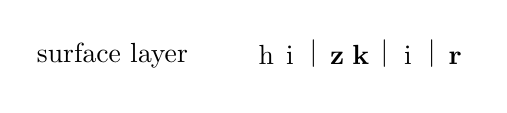
\begin{tikzpicture}[shorten >=1pt,draw=black!100]

	\def \floor{0cm}
	\tikzstyle{f-node}=[text height=6pt,text centered,inner sep=6pt,minimum size=15pt]
	\tikzstyle{annot}=[text width=20ex]
	% labels
	\node[annot] (floorlabel) at (0cm,\floor) {surface layer};
	
	% surface layer
	\node[f-node] 	(f0)	at (1.4cm,\floor)		{h};
	\node[f-node] 	(f1)	at (1.7cm,\floor)		{i};
	\node[f-node] 	(f2)	at (2cm,\floor)		{$|$};
	\node[f-node] 	(f3)	at (2.3cm,\floor)		{\textbf{z}};
	\node[f-node] 	(f4)	at (2.6 cm,\floor)	 	{\textbf{k}};
	\node[f-node] 	(f5)	at (2.9 cm,\floor)	 	{$|$};
	\node[f-node] 	(f6)	at (3.2 cm,\floor)	 	{i};
	\node[f-node] 	(f7)	at (3.5 cm,\floor)	 	{$|$};
	\node[f-node] 	(f8)	at (3.8 cm,\floor)	 	{\textbf{r}};
	\end{tikzpicture}
	\label{subfig:linear}
	}
\caption{Two approaches to analyzing \textit{hizkir} (`he reminded'), which has three morphemes. 
The root \textit{z-k-r} (boldface) is discontinuous. The linear (single-tier) approach is unable to connect the \textit{r} to the \textit{zk}, while the multilinear approach is able to unite discontiguous elements through external morpheme ($\mu$) nodes.}
%: an input layer ($\mathbf{d}$), a hidden layer ($\mathbf{m}$), and an output layer
\label{fig:approaches}
\end{figure}

% Describe how autosegmental theory reduces to a bipartite graph. 
In an autosegmental representation, each morph tier is a complex object, consisting of a particular sequence of phonological feature matrices, e.g., [-front,+low,-round,+syllabic]. However, one can generally use phonemic symbols as shorthand for
feature matrices; e.g., the feature matrix [-front,+low,-round,+syllabic] can be written as \textipa{/a/}. A sequence of feature matrices can thus be reduced to a sequence of alphabetic characters, each of which represents a particular set of features. For example, in figure~\ref{subfig:multilinear}, one morph is represented as the sequence \textipa{/hi/}, which is an abbreviation of \textipa{/}[+spread glottis][+front,-low,-round,+syllabic]\textipa{/}.
When feature matrices represented by /h/ and /i/ become linked to the first C and the first V, respectively, the C and V inherit these same feature matrices, which means that /h/ and /i/ can now also stand in for the initial C and V (respectively). 

A CV skeleton becomes a sequence of fully fledged phonemes, i.e., a phonological
form, as soon as morph tiers connect to its C and V slots, and it does so by taking 
on the identities of the phonological elements that compose the morphs. 
Thus, just as \textipa{/hi/} and \textipa{/i/} (i.e, the feature bundles they represent) compose 
$\mu_1$ in figure~\ref{subfig:multilinear}, they also now compose a morphological 
unit within the segmental tier. The morphs $\mu_1$, $\mu_2$, and $\mu_3$ 
essentially \emph{cause} the segmental tier to be realized as a fully fledged 
phonological form. These observations with become particular relevant in section~\ref{sec:mcmm-bipart} 
below as the following chapter, for we are coming close to describing the workings 
of \ac{MCMM}. 

%One might thus object to the simplicity of figure~\ref{subfig:multilinear}, e.g., its denoting the autosegmental morph tiers as $mu1$, etc., as though they were atomic units. But these labels are merely a form of shorthand. That is, one can generally use phonemic symbols as shorthand for
%feature matrices; e.g., the feature matrix [+back,+low, -cons] can be written as /a/
%%is a set of mutually nonadjacent nodes, where   
%each node is a bundle phonological features, e.g., [+back,+low, +syllabic]. However, one can generally use phonemic symbols as shorthand for
%feature bundles (or matrices); e.g., the feature matrix [+back,+low, +syllabic] can be written as /a/. 
%as  

These features are mapped onto the
C and V slots in McCarthy's segmental tier. 
 Each node, therefore, is complex.
But note that each morpheme tier can be represented abstractly as a single node; that is, 
its component nodes need not be represented explicitly 
because they are given by the edges linking the morpheme to the phonological segments.
We can thus view all the morpheme tiers as composing a single tier, with each morpheme represented as a single node in this tier.
We shall call this morph tier the \emph{hidden} \emph{layer}, the segmental tier the \emph{surface} \emph{layer}. 
In this way, the autosegmental multi-linear framework can be represented as a bipartite graph.

For convenience, we restate these properties here as (\ref{ex:criteria1-again}) and (\ref{ex:criteria2-again}):
\begin{exe} \label{ex:criteria-again} \ex \begin{xlist}
	\ex {\textsc{Nonlinearity}}.  %A model is \emph{nonlinear} 
	Morphs must be represented separately 
	from the surface (or phonological) tier, i.e., as residing on tiers distinct from 
	the phonological tier. \label{ex:criteria1-again}%eparately for m  as being separate from (or outside of) the the phonological (or segmental) tier.  % is a property wherein morphs are represented as being separate from the segmental tier.
	\ex {\textsc{Nonsequentiality}}.
	Each morph tier is required to be orthogonal to all other morph tiers. \label{ex:criteria2-again}
	\end{xlist}
\end{exe}
Fig.~\ref{fig:bipartite} is a bipartite
graph; its nodes are divided into two partitions, namely the sets $M$
and $R$. Within each set, all nodes are independent; 
the only connections are between nodes of different sets.

In graph-theoretic terms, the multi-linear formalism of
\cite{mccarthy:1981} is a type of \emph{multipartite}
graph. This is a graph whose nodes can be partitioned into two sets whose members are \emph{mutually nonadjacent}; i.e., no two nodes within the same set are connected by an edge.
%\emph{mutually nonadjacent}, i.e., disconnected, nodes; i.e., there are no connections between nodes of the same set. %two sets such that whose defining characteristic is that no two nodes with
%nodes within the \emph{same} set are connected by an edge.
Fig.~\ref{fig:bipartite}, for example, shows a \emph{bipartite}
graph, i.e., a graph with two such partitions, namely the sets $M$
and $R$ in this case.
Within each set, or \emph{layer}, all nodes are independent; that is there are no
intra-layer connections. The only connections are 
between nodes of different sets.

 \begin{figure}[htb]
 \begin{center}
 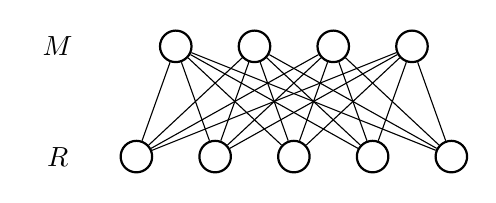
\begin{tikzpicture}[draw=black!100,scale=1.0]
 	\def \rowtwoht{1.4cm}
 	\def \rowoneht{0.0cm}
 	\tikzstyle{m-node}=[circle,draw=black!100,thick,inner sep=0pt,minimum size=4mm]
 	\tikzstyle{r-node}=[circle,draw=black!100,thick,inner sep=0pt,minimum size=4mm]
 	\tikzstyle{annot} = [text width=1.5em, text centered]
 	\node[annot] (hidden-label) at (-0.5cm,\rowtwoht) {$M$};
 	\node[annot] (surface-label) at (-0.5cm,\rowoneht) {$R$};
 	\node[m-node] 	(m0)	at (1cm,\rowtwoht)		{};
 	\node[m-node] 	(m1)	at (2cm,\rowtwoht)		{};
 	\node[m-node] 	(m2)	at (3cm,\rowtwoht)	 	{};
 	\node[m-node] 	(m3)	at (4cm,\rowtwoht) 		{};
 	% surface layer
 	\node[r-node] 	(r0)	at (0.5cm,\rowoneht)		{};
 	\node[r-node] 	(r1)	at (1.5cm,\rowoneht)		{};
 	\node[r-node] 	(r2)	at (2.5cm,\rowoneht)	 	{};
 	\node[r-node] 	(r3)	at (3.5cm,\rowoneht) 		{};
 	\node[r-node] 	(r4) 	at (4.5cm,\rowoneht)   		{};
 	%\node[r-node] 	(r5) 	at (6.5cm,\rowoneht)   		{};
 	\path (r0)	edge	node	{}	(m0)
		(r0)	edge	node	{}	(m1)
		(r0)	edge	node	{}	(m2)
		(r0)	edge	node	{}	(m3)

		(r1)	edge	node	{}	(m0)
		(r1)	edge	node	{}	(m1)
		(r1)	edge	node	{}	(m2)
		(r1)	edge	node	{}	(m3)

		(r2)	edge	node	{}	(m0)
		(r2)	edge	node	{}	(m1)
		(r2)	edge	node	{}	(m2)
		(r2)	edge	node	{}	(m3)
						
		(r3)	edge	node	{}	(m0)
		(r3)	edge	node	{}	(m1)
		(r3)	edge	node	{}	(m2)
		(r3)	edge	node	{}	(m3)

		(r4)	edge	node	{}	(m0)
		(r4)	edge	node	{}	(m1)
		(r4)	edge	node	{}	(m2)
		(r4)	edge	node	{}	(m3);
 		%(m3)	edge	node	{}	(r5);		
 \end{tikzpicture}
 \end{center}
 \caption{Bipartite graph}
 %. Neither layer contains sequential dependencies; every unit is independent within its own layer. Each hidden unit is thus free to cause any combination of observed units.}
 \label{fig:bipartite}
 \end{figure}

%This bipartiteness is important because many learning algorithms are based on bipartite graphs. I will be focusing on one such algorithm called
%the Multiple Cause Mixture Model (MCMM)
%\citep{saund:94}. An MCMM is a kind of autoencoder network with a bipartite architecture. It has two layers of nodes, a reconstruction (surface) layer $R$, where it attempts to reconstruct the input feature vectors, and a hidden layer whose nodes encode shared features among the input vectors. Weighted arcs link the nodes of one layer to those of the other, but there are no \emph{intra}-layer connections.

% Hebrew morphology, both its non-concatenative and concatenative components. 
%In a multi-linear framework, concatenative morphology is just a special case of non-concatenative morphology. There is no fundamental difference between them.
\section{An MCMM is a Bipartite Graph}\label{sec:mcmm-bipart}
An MCMM, as it turns out, is a special case of a bipartite graph. Indeed,
fig.~\ref{fig:bipartite} could itself be a simple MCMM. %precisely the architecture of an MCMM.
%To sum up, bipartite graphs possess the properties nonlinerarity and nonsequentiality. 
Because MCMMs are bipartite graphs, and bipartite graphs are both nonlinear and nonsequential, 
MCMMs must themselves be nonlinear and nonsequential, which makes MCMMs well-suited for modeling
non-concatenative morphology.

%As it turns out, 
A bipartite graph suffices
%we do not need many partitions 
to capture the essential properties of McCarthy's autosegmental
framework,
% (fig.~\ref{subfig:nonlinear}). 



\section{Conclusion}
\label{sec:mcmm-bipart}

That is, because of its bipartite properties, an MCMM provides a sound framework in which to implement autosegmental morphology, or at least the components of autosegmental morphology that address non-concatenative morphology.
An MCMM, as it turns out, is a special case of a bipartite graph. Indeed,
fig.~\ref{fig:bipartite} could itself be a simple MCMM. %precisely the architecture of an MCMM.
%To sum up, bipartite graphs possess the properties nonlinerarity and nonsequentiality. 
Because MCMMs are bipartite graphs, and bipartite graphs are both nonlinear and nonsequential, 
MCMMs must themselves be nonlinear and nonsequential, which makes MCMMs well-suited for modeling
non-concatenative morphology.

Because a bipartite graph meets the two criteria stated in
(\ref{ex:criteria}).  We can reformulate the morpheme tiers and the
segmental tier in fig.~\ref{subfig:nonlinear} as the sets $M$ and
$R$, respectively, in fig.~\ref{fig:bipartite} This satisfies the first
criterion. For the second, each node in $M$ represents a morpheme (or
morpheme tier), and, by the definition of \emph{bipartite}, the nodes
within $M$ are independent and thus orthogonal.

An MCMM (section~\ref{sec:mcmm}) is well-suited to learn 
non-concatenative morphology because it is bipartite graph. It has two
\emph{layers} (equivalently, sets) of nodes, a hidden layer and a
surface layer---corresponding, respectively, to $M$ and $R$ in
fig.~\ref{fig:bipartite}. There are no intra-layer connections in an
MCMM, only connections between layers.
%, as in any bipartite graph.

We shall henceforth refer to an MCMM's partitions as
\emph{vectors}, i.e., vectors of nodes, and use matrix and vector notation to
describe the components of an MCMM:
In particular, 
uppercase boldface letters will denote matrices, %(e.g., $\mathbf{M}$),
lowercase boldface letters will denote vectors,
% and matrix rows or columns, 
%(e.g., $\mathbf{m}_i$),
and italicized lowercase letters refer to the individual elements
of vectors/matrices. % (e.g., $m_{ik}$).
For example, $m_{i,k}$ is the $k^{\text{th}}$ element in the vector
$\mathbf{m}_i$, which is the $i^{\text{th}}$ row in the $I \times K$ matrix
$\mathbf{M}$. Thus, we shall henceforth write the $M$ and $R$ in
fig.~\ref{fig:bipartite} as $\mathbf{m}$ and $\mathbf{r}$,
respectively (or $\mathbf{m}_i$ and $\mathbf{r}_i$, where $i$ is the
index of the $i^{\text{th}}$ word). % Graph-Theoretic Foundation
\chapter{The Multiple Cause Mixture Model}
\label{ch:MCMM}

\section{Introduction}
\label{sec:mcmm:intro}
This chapter will focus on Multimorph's learning model, i.e. the principles and mechanisms that
enable it to learn. By \emph{model}, 
we mean a set of assumptions about the way the world works. In the case of Multimorph, 
the ``world" is the morphology of natural languages, which includes non-concatenative morphology. 
That is, is handle concatenative and non-conconcatenative morphology together, 
in a unified a way, as does
autosegmental morphology \citep{mccarthy:1981}. Recall from chapter~\ref{ch:graph} 
that in order
for a model to be able to non-concatenative morphology, it must be both \textbf{nonlinear}
 \textbf{nonsequential},i.e., satisfy the \textsc{Nonlinearity} and \textbf{Nonsequentiality} 
 criteria; 
 see definitions (\ref{def:nl}, \ref{def:ns}) and 
 proposition (\ref{prop:nlns}). Recall also that this 
 means that we need a bipartite graph. The Multiple Cause Mixture Model (MCMM) is a general 
 framework for unsupervised learning developed by \cite{saund:94}. Crucially, it is 
 a bipartite graph, and thus it can be
applied to the case of Multimorph.  

In what follows, we shall first, in section~\ref{sec:architecture}, discuss the architecture of an \ac{MCMM},
i.e., is key components and the relationships between these components. We shall then, in 
sections~\emph{mixing function} and \ref{sec:mcmm:learning}, describe how
learning takes place in an \ac{MCMM}. 

\section{Architecture}
\label{sec:architecture}
An MCMM is a graphical model consisting of two layers of nodes (or units): a layer 
of surface units 
and a layer of hidden, 
or causal, units. This is illustrated in fig.~\ref{fig:mcmm}, where $\mathbf{m}$ 
is the vector of hidden units, and $\mathbf{r}$ the vector of (reconstructed) surface units.
The hidden units are connected to surface units by a matrix of weights $\mathbf{C}$. 
Each individual arc $c_{j,k}$ has a value in $[0,1]$ that represents the weight on the connection between
$m_k$ and $r_j$.
Each node, i.e., each hidden unit and each surface unit, has an activity value in $[0,1]$ that
%Each hidden unit has an activity value in $[0,1]$ 
indicates whether it is \textsc{on} (active) or \textsc{off} (inactive).
The activity of $r_j$ is determined by a \emph{mixing function}, which takes as inputs the 
hidden-unit activities $\mathbf{m}$ and their respective weights $\mathbf{c}_j$
(section~\ref{sec:mixing-function}).

\begin{figure}[tb]
%\begin{minipage}{.3\textwidth}
\begin{center}
\small
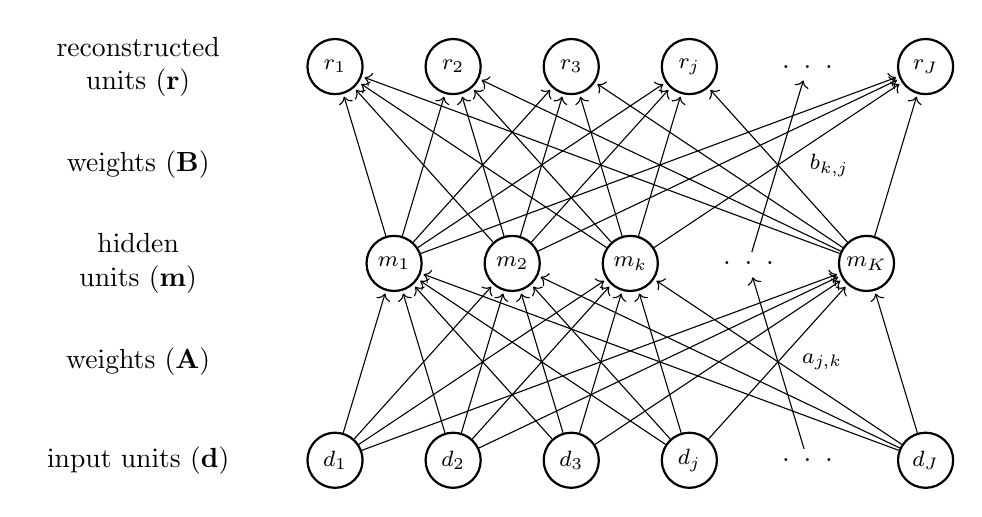
\begin{tikzpicture}[shorten >=1pt,->,draw=black!100]
	\def \rowtwoht{5cm}
	\def \weightstwo{3.75cm}
	\def \rowoneht{2.5cm}
	\def \weightsone{1.25cm}
	\def \basement{0cm}
	\tikzstyle{m-node}=[circle,draw=black!100,thick,inner sep=0pt,minimum size=7mm]
	\tikzstyle{r-node}=[circle,draw=black!100,thick,inner sep=0pt,minimum size=7mm]
	\tikzstyle{d-node}=[circle,draw=black!100,thick,inner sep=0pt,minimum size=7mm]
	\tikzstyle{dots}=[text width=5ex, text centered]
	\tikzstyle{annot}=[text width=17ex, text centered]
	% labels
	\node[annot] (r-layer) at (0cm,\rowtwoht) {reconstructed units ($\mathbf{r}$)};
	\node[annot] (weights) at (0cm,\weightstwo) {weights ($\mathbf{B}$)};
	\node[annot] (hidden-layer) at (0cm,\rowoneht) {hidden units ($\mathbf{m}$)};
	\node[annot] (weights) at (0cm,\weightsone) {weights ($\mathbf{A}$)};
	\node[annot] (d-layer) at (0cm,\basement) {input units ($\mathbf{d}$)};
	
	\node[dots] 	(m3)	at (7.75cm,\rowoneht)	 	{. . .};
	\node[dots] 	(r4) 	at (8.5cm,\rowtwoht)   		{. . .};
	\node[dots] 	(d4) 	at (8.5cm,\basement)   		{. . .};
	
	\footnotesize
	% hidden layer
	\node[m-node] 	(m0)	at (3.25cm,\rowoneht)		{$m_1$};
	\node[m-node] 	(m1)	at (4.75cm,\rowoneht)		{$m_2$};
	\node[m-node] 	(m2)	at (6.25cm,\rowoneht)	 	{$m_k$};
	\node[m-node] 	(m4)	at (9.25cm,\rowoneht)	 	{$m_K$};
	
	% reconstructed vector
	\node[r-node] 	(r0)	at (2.5cm,\rowtwoht)		{$r_1$};
	\node[r-node] 	(r1)	at (4cm,\rowtwoht)		{$r_2$};
	\node[r-node] 	(r2)	at (5.5cm,\rowtwoht)	 	{$r_3$};
	\node[r-node] 	(r3)	at (7cm,\rowtwoht) 		{$r_j$};
	\node[r-node] 	(r5) 	at (10cm,\rowtwoht)   		{$r_J$};
	%\node[r-node] 	(r6) 	at (9.75cm,\rowoneht)   	{$r_J$};
	
	% data vector
	\node[d-node] 	(d0)	at (2.5cm,\basement)		{$d_1$};
	\node[d-node] 	(d1)	at (4cm,\basement)		{$d_2$};
	\node[d-node] 	(d2)	at (5.5cm,\basement)	 	{$d_3$};
	\node[d-node] 	(d3)	at (7cm,\basement) 		{$d_j$};
	\node[d-node] 	(d5) 	at (10cm,\basement)   		{$d_J$};
	%\node[d-node] 	(d6) 	at (9.75cm,\basement)   	{$d_J$};
	
	\path
		(d0)	edge	node	{}	(m0)
		(d0)	edge	node	{}	(m1)
		(d0)	edge	node	{}	(m2)
		%(d0)	edge	node	{}	(m3)
		(d0)	edge	node	{}	(m4)
		%	
		(d1)	edge	node	{}	(m0)
		(d1)	edge	node	{}	(m1)
		(d1)	edge	node	{}	(m2)
		%(d1)	edge	node	{}	(m3)
		(d1)	edge	node	{}	(m4)
		%
		(d2)	edge	node	{}	(m0)
		(d2)	edge	node	{}	(m1)
		(d2)	edge	node	{}	(m2)
		(d2)	edge	node	{}	(m4)
		%
		(d3)	edge	node	{}	(m0)
		(d3)	edge	node	{}	(m1)
		(d3)	edge	node	{}	(m2)
		(d3)	edge	node	{}	(m4)
		%
		(d4)	edge	node[right=2mm]	{$a_{j,k}$}	(m3)
		%
		(d5)	edge	node	{}	(m0)
		(d5)	edge	node	{}	(m1)
		(d5)	edge	node	{}	(m2)
		(d5)	edge	node	{}	(m4)
	 
		(m0)	edge	node	{}	(r0)
		(m0)	edge	node	{}	(r1)
		(m0)	edge	node	{}	(r2)
		(m0)	edge	node	{}	(r3)
		(m0)	edge	node	{}	(r5)

		(m1)	edge	node	{}	(r0)
		(m1)	edge	node	{}	(r1)
		(m1)	edge	node	{}	(r2)
		(m1)	edge	node	{}	(r3)
		(m1)	edge	node	{}	(r5)

		(m2)	edge	node	{}	(r0)
		(m2)	edge	node	{}	(r1)
		(m2)	edge	node	{}	(r2)
		(m2)	edge	node	{}	(r3)
		(m2)	edge	node	{}	(r5)

		(m3)	edge	node[right=3mm]	{$b_{k,j}$}	(r4)	
		
		(m4)	edge	node	{}	(r0)
		(m4)	edge	node	{}	(r1)
		(m4)	edge	node	{}	(r2)
		(m4)	edge	node	{}	(r3)
		(m4)	edge	node	{}	(r5);
		
\end{tikzpicture}
\end{center}
\caption{many-to-many}
%: an input layer ($\mathbf{d}$), a hidden layer ($\mathbf{m}$), and an output layer
\label{fig:autoencoder}
\end{figure}



%Both hidden nodes and surface nodes have activity values, i.e., values in $[0,1]$ that
%indicate whether a node is \textsc{on} (active) or \textsc{off} (inactive). Each surface-node activity 
%is a function of the hidden-node activities and the weights that connect the hidden nodes to the surface node in question.

%Each surface node is either \textsc{on} (active) or \textsc{off} (inactive) depending 
%on the hidden-node activities and
%the weights connecting hidden nodes to surface nodes. 

%\subsection{Architecture}
%\label{subsec:architecture}

An MCMM can be viewed as a variant of the classical autoencoder
network \citep{dayan-and-zemel:95}, a type of neural network used for
unsupervised learning.  In autoencoders, a hidden layer is forced to
learn a compression scheme, i.e., a lower-dimensional encoding, for
a dataset.
 
%MCMMs are called \emph{Multiple Cause} Mixture Models because more
%than one hidden unit can take part in the activation of a surface
%unit.  
%This is illustrated in figure \ref{fig:mcmm}, where the nodes
%$\mathbf{m}$ are the hidden units, and $\mathbf{r}$ is the (reconstructed) surface
%vector.
%Each arc $c_{j,k}$ represents the weight on the connection between
%$m_k$ and $r_j$.
%The activity of $r_j$ is determined by a mixing function 
%(section~\ref{sec:mixing-function}).

\begin{figure}[htb]
\begin{center}
\small
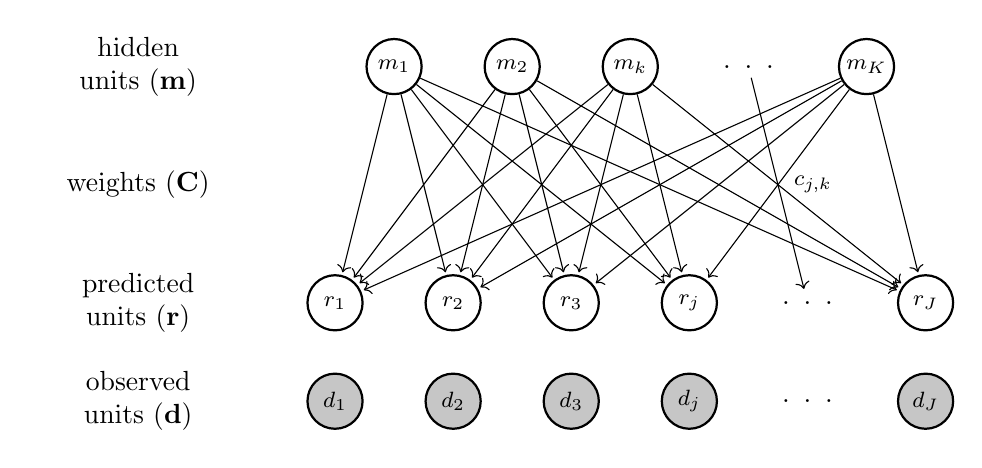
\begin{tikzpicture}[shorten >=1pt,->,draw=black!100]
	\def \rowtwoht{4.25cm}
	\def \weightlevel{2.75cm}
	\def \rowoneht{1.25cm}
	\def \basement{0cm}
	\tikzstyle{m-node}=[circle,draw=black!100,thick,inner sep=0pt,minimum size=7mm]
	\tikzstyle{r-node}=[circle,draw=black!100,thick,inner sep=0pt,minimum size=7mm]
	\tikzstyle{d-node}=[circle,draw=black!100,fill=gray!45,thick,inner sep=0pt,minimum size=7mm]
	\tikzstyle{dots}=[text width=5ex, text centered]
	\tikzstyle{annot}=[text width=17ex, text centered]
	% labels
	\node[annot] (hidden-layer) at (0cm,\rowtwoht) {hidden units ($\mathbf{m}$)};
	\node[annot] (weights) at (0cm,\weightlevel) {weights ($\mathbf{C}$)};
	\node[annot] (r-layer) at (0cm,\rowoneht) {predicted units ($\mathbf{r}$)};
	\node[annot] (d-layer) at (0cm,\basement) {observed units ($\mathbf{d}$)};
	
	\node[dots] 	(m3)	at (7.75cm,\rowtwoht)	 	{. . .};
	\node[dots] 	(r4) 	at (8.5cm,\rowoneht)   		{. . .};
	\node[dots] 	(d4) 	at (8.5cm,\basement)   		{. . .};
	
	\footnotesize
	% hidden layer
	\node[m-node] 	(m0)	at (3.25cm,\rowtwoht)		{$m_1$};
	\node[m-node] 	(m1)	at (4.75cm,\rowtwoht)		{$m_2$};
	\node[m-node] 	(m2)	at (6.25cm,\rowtwoht)	 	{$m_k$};
	\node[m-node] 	(m4)	at (9.25cm,\rowtwoht)	 	{$m_K$};
	
	% reconstructed vector
	\node[r-node] 	(r0)	at (2.5cm,\rowoneht)		{$r_1$};
	\node[r-node] 	(r1)	at (4cm,\rowoneht)		{$r_2$};
	\node[r-node] 	(r2)	at (5.5cm,\rowoneht)	 	{$r_3$};
	\node[r-node] 	(r3)	at (7cm,\rowoneht) 		{$r_j$};
	\node[r-node] 	(r5) 	at (10cm,\rowoneht)   		{$r_J$};
	%\node[r-node] 	(r6) 	at (9.75cm,\rowoneht)   	{$r_J$};
	
	% data vector
	\node[d-node] 	(d0)	at (2.5cm,\basement)		{$d_1$};
	\node[d-node] 	(d1)	at (4cm,\basement)		{$d_2$};
	\node[d-node] 	(d2)	at (5.5cm,\basement)	 	{$d_3$};
	\node[d-node] 	(d3)	at (7cm,\basement) 		{$d_j$};
	\node[d-node] 	(d5) 	at (10cm,\basement)   		{$d_J$};
	%\node[d-node] 	(d6) 	at (9.75cm,\basement)   	{$d_J$};
	
	\path 
		(m0)	edge	node	{}	(r0)
		(m0)	edge	node	{}	(r1)
		(m0)	edge	node	{}	(r2)
		(m0)	edge	node	{}	(r3)
		(m0)	edge	node	{}	(r5)
		
		(m1)	edge	node	{}	(r0)
		(m1)	edge	node	{}	(r1)
		(m1)	edge	node	{}	(r2)
		(m1)	edge	node	{}	(r3)
		(m1)	edge	node	{}	(r5)
		
		(m2)	edge	node	{}	(r0)
		(m2)	edge	node	{}	(r1)
		(m2)	edge	node	{}	(r2)
		(m2)	edge	node	{}	(r3)
		(m2)	edge	node	{}	(r5)
		(m3)	edge	node[right=1mm]	{$c_{j,k}$}	(r4)
		%	
		(m4)	edge	node	{}	(r0)
		(m4)	edge	node	{}	(r1)
		(m4)	edge	node	{}	(r2)
		(m4)	edge	node	{}	(r3)
		(m4)	edge	node	{}	(r5);
		
\end{tikzpicture}
\end{center}
\caption{Architecture of a Multiple Cause Mixture Model (MCMM)} 
\label{fig:mcmm}
\end{figure}


\begin{figure}[htb]
\begin{center}
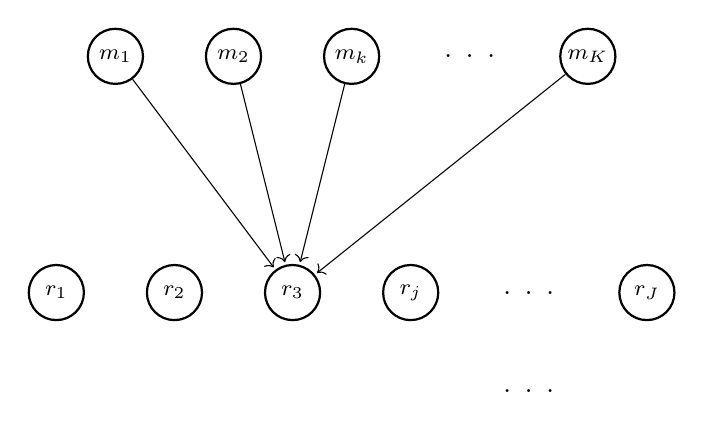
\begin{tikzpicture}[shorten >=1pt,->,draw=black!100]
	\def \rowtwoht{4.25cm}
	\def \weightlevel{2.75cm}
	\def \rowoneht{1.25cm}
	\def \basement{0cm}
	\tikzstyle{m-node}=[circle,draw=black!100,thick,inner sep=0pt,minimum size=7mm]
	\tikzstyle{r-node}=[circle,draw=black!100,thick,inner sep=0pt,minimum size=7mm]
	%\tikzstyle{d-node}=[circle,draw=black!100,fill=gray!45,thick,inner sep=0pt,minimum size=7mm]
	\tikzstyle{dots}=[text width=5ex, text centered]
	%\tikzstyle{annot}=[text width=17ex, text centered]
%	% labels
%	\node[annot] (hidden-layer) at (0cm,\rowtwoht) {hidden units ($\mathbf{m}$)};
%	\node[annot] (weights) at (0cm,\weightlevel) {weights ($\mathbf{C}$)};
%	\node[annot] (r-layer) at (0cm,\rowoneht) {predicted units ($\mathbf{r}$)};
	%\node[annot] (d-layer) at (0cm,\basement) {observed units ($\mathbf{d}$)};
	
	\node[dots] 	(m3)	at (7.75cm,\rowtwoht)	 	{. . .};
	\node[dots] 	(r4) 	at (8.5cm,\rowoneht)   		{. . .};
	\node[dots] 	(d4) 	at (8.5cm,\basement)   		{. . .};
	
	\footnotesize
	% hidden layer
	\node[m-node] 	(m0)	at (3.25cm,\rowtwoht)		{$m_1$};
	\node[m-node] 	(m1)	at (4.75cm,\rowtwoht)		{$m_2$};
	\node[m-node] 	(m2)	at (6.25cm,\rowtwoht)	 	{$m_k$};
	\node[m-node] 	(m4)	at (9.25cm,\rowtwoht)	 	{$m_K$};
	
	% reconstructed vector
	\node[r-node] 	(r0)	at (2.5cm,\rowoneht)		{$r_1$};
	\node[r-node] 	(r1)	at (4cm,\rowoneht)		{$r_2$};
	\node[r-node] 	(r2)	at (5.5cm,\rowoneht)	 	{$r_3$};
	\node[r-node] 	(r3)	at (7cm,\rowoneht) 		{$r_j$};
	\node[r-node] 	(r5) 	at (10cm,\rowoneht)   		{$r_J$};
	%\node[r-node] 	(r6) 	at (9.75cm,\rowoneht)   	{$r_J$};
	
	% data vector
%	\node[d-node] 	(d0)	at (2.5cm,\basement)		{$d_1$};
%	\node[d-node] 	(d1)	at (4cm,\basement)		{$d_2$};
%	\node[d-node] 	(d2)	at (5.5cm,\basement)	 	{$d_3$};
%	\node[d-node] 	(d3)	at (7cm,\basement) 		{$d_j$};
%	\node[d-node] 	(d5) 	at (10cm,\basement)   		{$d_J$};
	%\node[d-node] 	(d6) 	at (9.75cm,\basement)   	{$d_J$};
	
	\path 
		(m0)	edge	node	{}	(r2)
	
		(m1)	edge	node	{}	(r2)

		(m2)	edge	node	{}	(r2)
		%(m3)	edge	node {}	(r4)
		%(m3)	edge	node[right=1mm]	{$c_{j,k}$}	{}	(r0)
		%	
		(m4)	edge	node	{}	(r2);

		
\end{tikzpicture}
\end{center}
\caption{Architecture of a Multiple Cause Mixture Model (MCMM)} 
\label{fig:voting}
\end{figure}

%From source: "One  can  qualitatively  understand  the  difference  between  mixtures  and  products  by  observing  that  amixture distribution can have high probability for eventxwhen only a single expert assigns high probabilityto that event.  In contrast, a product can only have high probability for an eventxwhen all experts assignhigh probability to that event.  Hence, metaphorically speaking, a single expert in a mixture has the powerto pass a bill while a single expert in a product has the power to veto it.Put another way, each component in a product represents a softconstraint, while each expert in a mixturerepresents a soft template or prototype. For an event to be likely under a product model, all constraints must1
%be (approximately) satisfied, while an event is likely under a mixture model if it (approximately) matcheswith  a  single  template."

%Bishop: "One approach is to apply gradient-based optimization techniques (Fletcher, 1987;Nocedal and Wright, 1999; Bishop and Nabney, 2008). Although gradient-basedtechniques are feasible, and indeed will play an important role when we discussmixture density networks in Chapter 5, we now consider an alternative approachknown as the EM algorithm which has broad applicability and which will lay thefoundations for a discussion of variational inference techniques in Chapter 10." p. 435

%% Quora: "LDA is not a mixture model.  It is an admixture model or a mixed-membership model.
%Mixture models have a single latent variable that denotes which cluster they're in.  This is often written as an indicator variable z.  
%LDA is a model over documents (a bag of words), and has a latent variable for topic assignments for every token:  z1…zN
%Thus, words can belong to different clusters.  This intuitively makes sense because documents can be about more than one thing.  I.e., about both technology and business.  This often results in better models of real text than pure mixture models."

%The MCMM learns by comparing the reconstructed vector $\mathbf{r}_i$ 
%to its corresponding original datapoint $\mathbf{d}_i$. The discrepancy between
%the two is quantified by an \emph{objective function}. 
%If there is a discrepancy, the values of the nodes in
%$\mathbf{m}_i$ as well as the weights $\mathbf{C}$ are adjusted 
%in order to reduce the discrepancy as much as possible.
%See section~\ref{sec:mcmm-learning} for more on the learning process.

%Suppose data points $\mathbf{d}_u$ and $\mathbf{d}_v$ have some features in common.
%Then, as the MCMM tries to reconstruct them in $\mathbf{r}_u$ and $\mathbf{r}_v$, respectively,
%similarities will emerge between their respective hidden-layer vectors $\mathbf{m}_u$ and $\mathbf{m}_v$.
%In particular, the vectors $\mathbf{m}_u$ and
%$\mathbf{m}_v$ should come to share at least one active node, i.e., at least
%one $k \in K$ such that $m_{u,k} = 1$ and $m_{v,k} = 1$.
%This can serve as a basis for clustering;
%i.e., $m_{i,k}$ indicates whether $\mathbf{d}_i$ is a member of cluster $k$.
		
\section{Mixing Function}
\label{sec:mixing-function}

The mapping between the layer of hidden nodes $\textbf{m}$ 
and the layer of surface nodes $\textbf{r}$ is governed by a 
\emph{mixing function}, which is essentially
a voting rule \citep{saund:94}; it maps from a set of (weighted)
input ``votes'' to a single output decision.  The output decision is 
an activity value for a particular surface-layer node. We will call the input votes
\emph{causes}. 

In terms of architecture, the \ac{MCMM} bears a striking resemblance to the Restricted Boltzmann Machine (RBM) \citep{smolensky:1986}.
Both the \ac{MCMM} and the \ac{RBM} are bipartite graphs. That is both have two layers of nodes, with no connections between nodes of the same layer (as described in chapter~\ref{graph}).  In a RBM, as in an \ac{MCMM}, one of these node layers functions as a hidden layer, and the other as the visible (or surface) layer \citep[see, e.g.,][]{mohamed-and-hinton:2010}. One difference between the two, however, is that an RBM acts as a \emph{product} of experts, while an \ac{MCMM} acts as a kind of hybrid between a \emph{mixture of experts}, i.e., a (standard) mixture model, and a product of experts. To be clear, though, an \ac{MCMM} itself appears to be neither a sum nor a product of experts, not at least as these terms are usually construed. 

The ``experts" here 
%The RBM's equivalent of the MCMM's mixing function is a  \emph{product of experts}\citep{hinton:1999, hinton:2002}, where the ``experts" 
are the hidden units (along with their
respective weights). A product of experts is, as its name suggests, a multiplication, namely the product of all hidden-unit values, whereas a mixture of experts is a summation of these same values. In both MCMMs and RBMs, every expert casts a vote concerning whether a given surface node is to be \textsc{on} or \textsc{off} (i.e., 1 or 0). In an RBM, the votes are all multiplied together, so that if one vote is 0, the collective vote will be 0. In other words, in order for a given surface unit to be 1, \emph{every} hidden unit must vote 1.\footnote{If the values are continuous, i.e., in the interval $[0,1]$, every hidden unit must be very close to 1 in order for the surface unit to be close to 1.}
In an MCMM, by contrast, every expert save one could cast a 0 vote, and the surface unit's value would still be nonzero. As long as \emph{at least} one of the hidden-unit votes is 1, the surface unit in question will be 1. On the other hand, if multiple experts vote 1, the surface unit's value is still 1. It will not exceed one even if all hidden units vote 1. Thus, the \ac{MCMM}'s method of combining expert votes behaves like a summation in some ways and product in others.  

Because an \ac{MCMM} is not a true mixture of experts, it cannot be a true mixture model. In a true mixture model, the expert votes must always sum to 1, and each surface unit's value is a \emph{weighted sum} of the votes from the hidden units. As the number of votes increases, the potency of each vote tends to decrease, unless most votes have weights that are close to zero. Mixture-of-experts models perform best when each surface unit's value is caused by a single expert, namely the best expert for that surface unit. Otherwise, the best expert's vote will be dampened. (CITE?). By contrast, in an \ac{MCMM}, a particular surface unit can be caused by one expert, all experts, or any number in between (where, again, the experts are hidden units).
An \ac{MCMM} is in this way similar to an \emph{admixture} model like Latent Dirichlet Allocation (LDA) \citep{blei-et-al:2003}; e.g., 
when used in document classification, LDA %are applied to topic modeling, an individual word %(a surface unit) 
%can be 
can attribute a single word to multiple topics, %(hidden units).
which is to say that the word in question is \emph{caused} by multiple topics at once.
That is, a given word, %e.g., %\emph{restaurant} 
can be \emph{caused} by more than one topic, 
where each topic is a cluster of words.
%\citep[e.g.,][]{miller-et-al:2016} 
%(and each cluster is represented as shared connections to a particular hidden unit). %The clusters would  \emph{food}, \emph{business}, and \emph{hospitality}, simultaneously.

Like LDA, MCMMs can been applied to document classification; \cite{sahami-et-al:96} use an \ac{MCMM} to group $I$ documents into $K$ clusters. Each Documents are represented as vectors $\textbf{x}_i$ of $J$ features. The features, i.e. surface units, each indicate the absence or presence of a particular word (cf. the $\textbf{x}$ vector in figure~\ref{fig:mcmm}). The topics in \cite{sahami-et-al:96} are represented as the MCMM's hidden units $\textbf{m}_i$. Documents are grouped into topic clusters by the learning process described below in section~\label{sec:mcmm:learning}.
% are analogous to the morphological clusters in the present work; i.e., they each correspond to a hidden unit in $\textbf{m}$. In particular, each hidden unit in$\textbf{m}_i$ is the activity of a particular cluster for the $i$th datapoint--i.e., the $i$th document in the case of \cite{sahami-et-al:96}, and the $i$th word in the present work. 

%work hidden nodes in the vectors $  in the hidden-unit vectors $ were represented as $K$-length hidden-unit vectors $\textbf{}$ document vector is thus analagous  wordsthe express purpose of mapping 
%particularly to map individual documents 
%each to multiple categories at once \cite{sahami-et-al:96}. %apply the \ac{MCMM} to 
By contrast, a true mixture model, such as \dots, is constrained to assigning each surface unit to a \emph{single} cause. In the case of 
document classification, this would mean each word (surface unit) could be attribute to no more than
one topic (or hidden unit). One might therefore describe any standard (i.e., true) 
mixture model as a \emph{single-cause} mixture model. 


Each cause is a product of the form $m_{i,k} c_{j,k}$ for $k \in K$.
There are thus a total of $K$ distinct causes for a given surface node $r_{i,j}$. 
If the cause $m_{i,h} c_{j,h}$, where $h \in K$, is equal to $1$ or surpasses some
threshold, then $m_{i,h} c_{j,h}$ is an active cause.
%The input votes, are the activities of the hidden nodes,
%i.e., the $K$-length vector $\mathbf{m}_i$,
%coupled with their respective weights, i.e., the $K$-length vector 
%$\mathbf{c}_j$. 
%Any differentiable function
%that maps from the vector pair $(\mathbf{m}_i, \mathbf{c}_j)$ 
%to an activity value for $r_{i,j}$ can in theory serve as a mixing function. 
%There are thus an infinite number of theoretically possible mixing functions.

%Following \cite{saund:94}, we use the 
%There are perhaps an infinite number of possible mixing functions. 
%Any function that maps from a set of votes 
%(and their respective weights) to a single output decision will suffice.
One possibility is the \textbf{Noisy-OR} function:
 \begin{equation}\label{eq:noisy-or}
  r_{i,j} = 1 - \prod\limits_{k} (1 - m_{i,k} c_{j,k})
 \end{equation}
% We will call the inputs to the Noisy-OR function \emph{causes}. Each cause is a product of the form $m_{i,k} c_{j,k}$. 
 The Noisy-OR function acts as a kind of \textit{OR} gate, or, to put it another way, an``at-least-one" gate. That is, the surface node $r_{i,j}$ is $1$ as long as \emph{at least one} cause is active.
 % (i.e., $m_{i,k} c_{j,k} = 1$ for at least one $k$ in $K$). 
 If two or more causes are active,
%$1$ (or $\ge$ than a threshold), 
$r_{i,j}$ is still going to be $1$. The output of Noisy-OR does not change as the number of active causes change, as long as there is at least one active cause.

Another possible mixing function is the \textbf{sigmoidal weighted sum}, the composition of the sigmoid function $S$ and the function $t_{i,j}$, which computes a weighted sum, i.e., the inner product of the cluster-activity vector $\mathbf{m}_i$ and the weight vector $\mathbf{c}_j$:

	\begin{align} %\label{eq:sigws}
	\label{eq:sig}
	r_{i,j} = S(t_{i,j}) &= \frac{1}{1 + e^{-t_{i,j}}} \quad %\\   %\qquad \text{where} \quad
	%\label{eq:ws}
	\text{where} \quad t_{i,j} = \sum_k m_{i,k} c_{j,k}
	\end{align}
This is the mixing (or activation) function that is typically used in classical autoencoders. 
Whereas the output of Noisy-OR is independent of the number of active causes (as long as there is at least one), the output of \eqref{eq:sig} DOES change with the number of active causes: The value $t_{i,j} = \sum_k m_{i,k} c_{j,k}$ is clearly going to increase as the number of active clusters increases.
%(i.e., products of the form $m_{i,k} c_{j,k}$ that equal $1$ or are greater than some threshold) 
As $t_{i,j}$ increases, $S(t_{i,j})$ will get closer to $1$; as %it
$t_{i,j}$ 
decreases, $S(t_{i,j})$ will get closer to $0$.


\section{Learning}
\label{sec:mcmm:learning}
%\label{autoencoder-learning}

% A data compression scheme is useful only to the extent that it allows
% for the recovery of the source data from the compressed
% representations. In autoencoder terms, this means that 

%The reconstruction layer attempts to
%decode the hidden layer's representations and
In both the classical autoencoder and the MCMM, learning occurs as a
result of the algorithm's search for an optimal valuation of key variables (e.g., weights), 
i.e., a valuation that minimizes %or maximizes an the
%\emph{reconstruction error} $E$, 
the discrepancy between
reconstructed and original data points.  The search is conducted
via %some method of 
numerical optimization; we use the nonlinear conjugate gradient method.
%gradient-based technique, e.g., gradient descent or
%the conjugate gradient method.
%
Our objective function is a simple error function, namely the
normalized sum of squares error:
\begin{equation}
E = \frac{1}{I \times J} \sum_{i} \sum_{j} {(r_{i,j} - d_{i,j})}^2
\end{equation}
 where $I \times J$ is the total number of features in the dataset.
The MCMM's task is to minimize this function by adjusting the
 values in $\mathbf{M}$ and $\mathbf{C}$, where
 %$I \times $ matrix $\mathbf{M}$ and the $J \times K$ matrix $\mathbf{C}$.
$\mathbf{M}$ is the $I \times K$ matrix that
% of dimensions $I \times K$,
encodes each data point's cluster-activity vector, 
and $\mathbf{C}$ is the $J \times K$ matrix that
%, of dimensions $J \times K$, 
encodes the weights between $\mathbf{m}_i$ and $\mathbf{r}_i$ for every $i \in I$ (see fig.~\ref{fig:example}). 
%$\mathbf{C}$ can also be interpreted as encoding the cluster centroids 
%(the clusters' ``average'' data points).
%Each column in $\mathbf{C}$ is in effect a feature vector; the $k^{\text{th}}$ column is 
%the $k^{\text{th}}$ cluster's average feature vector.
% \begin{align*}
% 	% E &= \frac{1}{I} \sum_{i} e_{i} \\
% 	% e_{i} &= \frac{1}{J} \sum_{j} {(r_{i,j} - d_{i,j})}^2
% 	E &= \frac{1}{I \times J} \sum_{i} \sum_{j} {(r_{i,j} - d_{i,j})}^2
% \end{align*}
% %\marginpar{Rationale for normalized SSE?} 
% which is minimized.
% rather than maximized.  


%; our techniques are described in section~\ref{subsec:objfunc}.
% There are a number of possibilities regarding the particular error
% function and gradient-based technique. We describe our choices in
% section~\ref{subsec:objfunc}.
% Any information loss in the compression will result in reconstructed
% vectors that differ from the original data points.  This is called
%the \emph{reconstruction error} is measured by some error function
%$err$, such as the
%%.  A typical error function is 
%the sum of squared error ($err_i = \sum_{j}{(d_{i,j} -
%  r_{i,j})}^2$). The global reconstruction error $E$, for the whole
%dataset, is the sum of all $err_i$.
%% over $i \in I$.
%%
%To discover a compression scheme with a minimal $E$, autoencoders
%use gradient-based search techniques, e.g., gradient descent or the
%conjugate gradient method.  We describe our error function in
%section~\ref{subsec:objfunc}.

% The autoencoder's goal is to discover a compression scheme that causes a minimal $E$, 
% and since $E$ is ultimately a function of $\mathbf{A}$ and $\mathbf{B}$, 
% this task reduces to finding the valuations for $\mathbf{A}$ and $\mathbf{B}$ that minimize $E(\mathbf{A},\mathbf{B}$). To this end, autoencoders use gradient-based search techniques, e.g., gradient descent or the conjugate gradient method. In the remainder of this section, we provide a very general description of an autoencoder's weight updating process. The details, especially the specific form of the weight-update function, depend on the particular gradient-based technique used. 

% Taking as input the data points $\mathbf{d}_i \in \mathbf{D}$, the network yields a reconstructed vector $\mathbf{r}_i$ for each individual $\mathbf{d}_i$. Because $\mathbf{D}$ contains $I$ data points, one epoch (i.e., one cycle through the dataset) is complete after $I$ iterations, whereupon ${E}(\mathbf{A}, \mathbf{B})$ is calculated, and each weight in $\mathbf{A}$ and $\mathbf{B}$ is adjusted in a way that furthers the descent of $E$ toward a minimum. 
% In particular, the algorithm adds to each 
% $b_{k,j} \in \mathbf{B}$ a quantity proportional to the negative gradient of 
% $E$ at $b_{k,j}$, or $-\frac{\partial E}{\partial b_{k,j}}$. 
% It similarly adds to each $a_{j,k} \in \mathbf{A}$
% a quantity proportional to the negative gradient of $E$ at $a_{j,k}$,
% or $-\frac{\partial E}{\partial a_{j,k}}$.
% These weight updates serve to improve the network's compression model, so that each successive epoch yields a smaller reconstruction error than the preceding epoch.
% The succession of epochs continues until $E$ falls below some small predesignated value.


% \subsection{The MCMM as an autoencoder variant}
% \label{subsec:mcmm-variant}

%\subsubsection{Architecture}
% Like the classical autoencoder, the MCMM has a hidden layer $\mathbf{m}$ and a reconstruction layer $\mathbf{r}$, as illustrated in figure \ref{fig:mcmm}. 
% However, the MCMM does not have an explicit
% data (or input) layer corresponding to the classical autoencoder's $\mathbf{d}$.
% Because the MCMM has only a two layers of nodes instead of three, it needs only a single layer of connecting weights, namely the weight matrix $\mathbf{C}$. This is a $J \times K$ matrix,
% since there are $K$ nodes in $\mathbf{m}$ and $J$ nodes in $\mathbf{r}$,
% and every $m_k$ must be linked to every $r_j$.

%\subsubsection{Mixing Function}
% MCMMs are distinguished by their propensity for learning hidden-unit activations and weight configurations that have clear interpretations.

% In the classical autoencoder, the activity $\phi(net)$ of any node $y$ is a
% function of its net raw input $net_y$, which is the weighted sum of $y$'s
% individual input signals (see \eqref{weighted-sum}). 
% The logistic sigmoid function $\phi$ then scales ${net}_y$ so that it falls within $[0,1]$.

% \begin{align*}
% r_{j} &= \sigma({net}_j) \\
% &= \sigma\big(\sum_k b_{k,j} \cdot m_k \big) \\
% &= \sigma \bigg(\sum_k b_{k,j} \cdot \sigma \big({net}_k \big) \bigg) \\
% &= \sigma \bigg(\sum_k b_{k,j} \cdot \sigma \big(\sum_j a_{j,k} \cdot d_j \big) \bigg) \\
% \end{align*}
% The activity of any given reconstruction node $r_j$ depends not only on the weights $\mathbf{B}$, but also on the weights $\mathbf{A}$.
% Moreover, $\mathbf{A}$ and $\mathbf{B}$ may differ.
% When $\mathbf{A} \ne \mathbf{B}$, the $\mathbf{B}$ weights can counteract the effects of the $\mathbf{A}$ weights, giving rise to unexpected activities among the $\mathbf{m}$ units and obscuring the  
% relationships between the $\mathbf{m}$ units and the $\mathbf{r}$ units.

% The MCMM, in contrast, is designed with the express purpose of providing a coherent causal explanation for regularities in surface data.
% What makes this possible?
% \begin{itemize} 
% \item \textit{Binary activities and weights.} Both the weights and the hidden unit activities are constrained to stay in $[0,1]$. At convergence, moreover, all values---both weights and hidden activities---should be either $0$ or $1$. \textit{Why is this important?} Binary values, i.e., \textsc{true} and \textsc{false}, have clear interpretations.
% \item \textit{Single layer of weights.} An MCMM has only one layer of weights. \textit{Why is this important?} The activities of the hidden units are manipulated directly in response to the reconstruction error.
% \item 
% \textit{How so?} In the classical autoencoder, the terms $m_kc_{j,k}, k \in K$ are combined linearly prior to sigmoid squashing. But MCMMs employ mixing functions such that the combination of these terms is nonlinear from the start. \textit{Why does this matter?} This ``total" nonlinearity encourages (?) weights to converge toward discrete values. The ultimate decision is then based on multiple discrete, either-or votes.
% \textit{Why, then, is clipping necessary?}
% \end{itemize}

% The classical autoencoder's activation function $\sigma({net}_y)$ is one possible mixing function,
% for it indeed takes the $K$ distinct input signals to node $y$ and yields a single activity value.
% However, as Saund points out, $\sigma({net}_y)$ is not well suited to the purpose of coherently distinguishing causes from non-causes. This is because $net_y$ is additive rather than multiplicative. Noisy-or is multiplicative:
% \begin{align*}
% r_{j} &= 1 - (1 - m_0c_{0,j}) \times (1 - m_1c_{1,j}) \times (1 - m_2c_{2,j}) \\
% &= 1 - (1 - 0) \times (1 - 0) \times (1 - 1) \\ 
% &= 1 - 1 \times 1 \times 0 \\
% &= 1
% \end{align*}
% As long as at least one $m_kc_{j,k} = 1$ (where $k = 0,1,\dots,K$), $r_{j}$ will be active,
% and $r_{j} = 0$ only if all products $m_kc_{j,k}$ are zero.
% Notice that $m_kc_{j,k} = 1$ only if both $m_k = 1$ and $c_{j,k} = 1$.
% On the other hand, with sigmoid squashing, $\sigma({net}_j)$ is never truly zero; it just gets infinitely close to zero.
% And $\sigma({net}_j)$ will be close to $1$ as long as ${net}_j = \sum_K m_k c_{j,k}$ is sufficiently large. 
% There are an infinite number of valuations for $\mathbf{m}$ and $\mathbf{c}_{j}$ that could give rise to a sufficiently large ${net}_j$.

% The function ${net}$ is an example of a linear mixing function. However, the autoencoder's mixing function
% is made nonlinear by $\phi({net}_y)$, which ``squashes" $net_y$ to fall within $[0,1]$.

%\subsubsection{Learning}
%\label{mcmm-learning}

%\paragraph{MCMM}

%\marginpar{MD: In fig.~\ref{fig:example}, we use $\mathbf{M}$, but
%  in previous figures we use $\mathbf{m}$.  Also, why is it sometimes
%  $\mathbf{m_k}$ and sometimes $\mathbf{m_{i,k}}$?  ($i$ refers to the
%  $i^{\text{th}}$ word?)}

The MCMM's learning process is similar to Expectation Maximization
(EM) in that at any given time it holds one set of variables 
fixed while optimizing the other set. We thus have two functions, \textsc{Optimize-M}
and \textsc{Optimize-C}, which take turns optimizing their respective matrices.
% However, if the algorithm is to optimize $\mathbf{M}$, it must first
% know $\mathbf{C}$, and vice versa.  Therefore, the algorithm can only
% focus on matrix at time, optimizing the one while holding the other
% fixed.
% The learning process consists of two distinct optimization
% functions:
%, \textsc{Optimize-M} and \textsc{Optimize-C}.
%\begin{description}
%\item[
% \textsc{Optimize-M} holds $\mathbf{C}$ fixed in order to optimize the
% cluster activity vectors in $\mathbf{M}$, while \textsc{Optimize-C}
% holds $\mathbf{M}$ fixed in order to optimize the cluster centroids in
% $\mathbf{C}$.
%\end{description}

The function \textsc{Optimize-M} visits each of the $I$ cluster-activity vectors $\mathbf{m}_i$ in
$\mathbf{M}$, optimizing each one separately.
%, one at a time.
%in $\mathbf{M}$, 
For each $\mathbf{m}_i$, \textsc{Optimize-M} enters an optimization 
loop over its $K$ components, adjusting each 
$m_{i,k}$ by a
quantity proportional to the negative gradient of $E$ at $m_{i,k}$. \marginpar{How is this proportion determined?} 
This loop repeats until $E$
ceases to decrease significantly,
whereupon \textsc{Optimize-M} proceeds to the next $\mathbf{m}_i$.  
The function \textsc{Optimize-C} consists of a single optimization loop over the 
entire matrix
$\mathbf{C}$. Each $c_{j,k}$ is adjusted by a quantity
proportional to the negative gradient of $E$ at $c_{j,k}$.
%, or $-\frac{\partial E}{\partial c_{j,k}}$.
%(in the case of gradient descent).  
%Since $E$ is simply
%$\sum_i e_i$, i.e., the sum of the errors of the individual data-point
%reconstructions, $-\frac{\partial E}{\partial c_{j,k}} = -\sum_i
%\frac{\partial e_i}{\partial c_{j,k}}$.  Thus, the adjustment to each
%$c_{j,k}$ takes into account the error of each reconstructed vector
%$\mathbf{r}_i$ in $\mathbf{R}$. However,
Unlike \textsc{Optimize-M}, which comprises $I$ separate optimization
loops, \textsc{Optimize-C} consists of just one, 
%optimizing the $\mathbf{C}$ matrix as a whole.  
When each of its $J \times K$
components has been adjusted, one round of updates to $\mathbf{C}$ is
complete.  $E$ is reassessed only between completed rounds of
updates. If the change in $E$ remains significant, another round begins.  
Both \textsc{Optimize-M} and \textsc{Optimize-C} are enclosed within 
an ``alternation loop" 
that alternates between the two functions, holding $\mathbf{C}$ fixed
during \textsc{Optimize-M}, and vice versa.
This alternation continues until $E$ cannot be decreased further. At
this point, an ``outer loop''
splits the cluster which contributes the most to the error, adds one
to the cluster count $K$, and restarts the alternation loop. The outer loop
repeats until it reaches an overall stopping criterion, e.g., $E = 0$.
%; otherwise, the function terminates.
 \subsection{Bound Constrained Optimization}
The optimization task is subject to the constraint %$0 le m_{i,k} ge 1$
that no value in $\mathbf{M}$ or $\mathbf{C}$ may exceed 1 or fall below 0. In other words,
it is a task of bound constrained optimization. Thus, whenever a value in either $\mathbf{M}$ or $\mathbf{C}$ is about
to fall below 0, it is set to 0. Likewise, whenever a value is about to exceed 1, it is set to 1
\citep{ni:yuan:1997}.
 %It repeatedly iterates over the $J \times K$ components of $\mathbf{C}$, stopping only when it finds a local minimum of $E$ is
  
%What is the inner loop and what is the outer loop?
%There are actually two inner loops: Opt-M is immediately followed by Opt-C. These two are encapsulated within a larger outer loop.
%What is the stopping criterion for the inner loop? What happens when this criterion is met?
%What is the stopping criterion for the outer loop?
%Cluster Splitting. Where does this enter the narrative?
%At this point, the algorithm then finds the worst cluster among the currently existing clusters and splits it, thereby increasing the cluster count $K$ by one.

\subsection{A Simple MCMM Example}
\label{subsec:example}

Fig.~\ref{fig:example} shows an example of an MCMM for two data points (i.e., $I = 2$).
The hidden cluster activities $\mathbf{M}$, the weights $\mathbf{C}$,
and the mixing function $r$ constitute a model that reproduces the
observed data points $\mathbf{D}$.
%
%\marginpar{MD: I don't quite understand the ``center vector''
  %statement}
%
The nodes $m_{i,k}$ represent cluster activities; if $m_{1,2} = 1$,
for instance, the second cluster is active for $\mathbf{d}_1$ (i.e.,
$\mathbf{d}_1$ is a member of cluster 2).
%
Note that the $J \times K$ weight matrix $\mathbf{C}$ is the same for
all data points, and
%
% For each data point, the arcs emanating from cluster
% 1 and cluster 2 represent the components of $\mathbf{C}$'s first and
% second rows, respectively. The $k$th row in $\mathbf{C}$ is thus
% uniquely associated with the $k$th cluster. Moreover, 
%
the $k^{\text{th}}$ row in $\mathbf{C}$ can be seen as the $k^{\text{th}}$
cluster's ``average" vector: the $j^{\text{th}}$ component in
$\mathbf{c}_k$ is 1 only if all data points in cluster $k$ have
1 at feature $j$.
%the $k^{\text{th}}$ row of $\mathbf{C}$ is in effect
%the center vector of the $k^{\text{th}}$ hidden cluster.
%
%In the figure, 

%\begin{figure}[htb!]
%\usetikzlibrary{positioning}
%%\begin{minipage}{.3\textwidth}
%\begin{center}
%%\subfigure[Learning in Progress]{
%\begin{tikzpicture}[shorten >=1pt,->,draw=black!100, scale=0.85]
%	\footnotesize
%%	\def \attic{5.95cm}
%%	\def \rowtwoht{5.4cm}
%%	\def \weightlevel{3.9cm}
%%	\def \rowoneht{2.4cm}
%%	\def \basement{1.8cm}
%%	\def \data{1cm}
%%	\def \china{0cm}
%
%	\def \attic{5.4cm}
%	\def \rowtwoht{4.8cm}
%	\def \weightlevel{3.6cm}
%	\def \rowoneht{2.4cm}
%	\def \basement{1.8cm}
%	\def \data{1cm}
%	\def \china{0cm}
%		
%	\tikzstyle{m-node}=[circle,draw=black!100,thick,inner sep=0pt,minimum size=6mm]
%	\tikzstyle{r-node}=[circle,draw=black!100,thick,inner sep=0pt,minimum size=6mm]
%	\tikzstyle{d-node}=[circle,draw=black!100,fill=gray!45,thick,inner sep=0pt,minimum size=6mm]
%	%\tikzstyle{dots}=[text width=5ex, text centered]
%	\tikzstyle{annot}=[text width=2.5em]
%	% labels
%	\tikzstyle{label}=[text width=2.5em, text centered]
%	\tikzstyle{formula}=[text width=30em, text centered]
%	
%	\scriptsize
%	\node[annot] (hidden-layer) at (0cm,\rowtwoht) {$\mathbf{M}_{(i,k)}$};
%	\node[annot] (weights) at (0cm,\weightlevel) {$\mathbf{C}_{(j,k)}$};
%	\node[annot] (r-layer) at (0cm,\rowoneht) {$\mathbf{R}_{(i,j)}$};
%	
%	% hidden layer
%	\scriptsize
%	\node[m-node] 	(ma00)	at (1.45cm,\rowtwoht)		{$.2$};
%	\node[m-node] 	(ma01)	at (3.35cm,\rowtwoht)		{$.9$};
%	\node[m-node] 	(ma10)	at (5.55cm,\rowtwoht) 	{$.8$};
%	\node[m-node] 	(ma11)	at (7.45cm,\rowtwoht)	 	{$.1$};
%	% \node[m-node] 	(m20)	at (9.65cm,\rowtwoht) 	{$.8$};
%	% \node[m-node] 	(m21)	at (11.55cm,\rowtwoht)	 	{$.9$};
%	
%	%\footnotesize
%	\node[label]	(ml00) 	at (1.45cm,\attic)		{$m_{1,1}$}; %1.75 -> 1.45
%	\node[label]	(ml01) 	at (3.35cm,\attic)		{$m_{1,2}$}; %3.05 -> 3.35
%	\node[label] 	(ml10)	at (5.55cm,\attic) 	{$m_{2,1}$};     %5.85 -> 5.55
%	\node[label] 	(ml11)	at (7.45cm,\attic)	 	{$m_{2,2}$}; %7.15 -> 7.45
%	% \node[label] 	(ml20)	at (9.65cm,\attic) 	{$m_{3,1}$};     %9.95 -> 9.65
%	% \node[label] 	(ml21)	at (11.55cm,\attic)	 	{$m_{3,2}$}; %11.25 -> 11.55
%	
%	\scriptsize
%	\node[r-node] 	(ra00)	at (1.1cm,\rowoneht)		{$.24$};
%	\node[r-node] 	(ra01)	at (2.4cm,\rowoneht)		{$.81$};
%	\node[r-node] 	(ra02)	at (3.7cm,\rowoneht)	 	{$.23$};
%	
%	\node[r-node] 	(ra10)	at (5.2cm,\rowoneht) 		{$.68$};
%	\node[r-node] 	(ra11) 	at (6.5cm,\rowoneht)   	{$.16$};
%	\node[r-node] 	(ra12)	at (7.8cm,\rowoneht)		{$.76$};
%	
%	% \node[r-node] 	(r20) 	at (9.3cm,\rowoneht)  		{$.71$};
%	% \node[r-node] 	(r21)	at (10.6cm,\rowoneht) 		{$.83$};
%	% \node[r-node] 	(r22) 	at (11.9cm,\rowoneht)   	{$.77$};
%	
%	\node[label] 	(rl00)	at (1.1cm,\basement)		{$r_{1,1}$};
%	\node[label] 	(rl01)	at (2.4cm,\basement)		{$r_{1,2}$};
%	\node[label] 	(rl02)	at (3.7cm,\basement)	 	{$r_{1,3}$};
%	
%	\node[label] 	(rl10)	at (5.2cm,\basement) 		{$r_{2,1}$};
%	\node[label] 	(rl11) 	at (6.5cm,\basement)   	{$r_{2,2}$};
%	\node[label] 	(rl12)	at (7.8cm,\basement)		{$r_{2,3}$};
%	
%%	\node[label] 	(rl20) 	at (9.3cm,\basement)  		{$r_{3,1}$};
%%	\node[label] 	(rl21)	at (10.6cm,\basement) 		{$r_{3,2}$};
%%	\node[label] 	(rl22) 	at (11.9cm,\basement)   	{$r_{3,3}$};
%
%	\draw[-] (4.45cm, \attic+1.5mm) -- (4.45cm, \basement-1.5mm);
%%	\draw[-] (8.55cm, \attic+1.5mm) -- (8.55cm, \basement-1.5mm);
%
%	\scriptsize
%	\path
%		(ma00)	edge	node [left]	{$.85$} (ra00)
%		(ma00)	edge	node [left,xshift=-1mm,yshift=3mm]	{$.1$}	(ra01)
%		(ma00)	edge	node [left,xshift=-1mm,yshift=8mm]	{$.95$}	(ra02)
%
%		(ma01)	edge	node [right,xshift=3mm,yshift=8mm]	{$.1$}	(ra00)
%		(ma01)	edge	node [right,xshift=1mm,yshift=3mm]	{$.9$}	(ra01)
%		(ma01)	edge	node [right]	{$.05$} (ra02)
%		%
%		(ma10)	edge	node [left] {$.85$} (ra10)
%		(ma10)	edge	node [left,xshift=-1mm,yshift=3mm]	{$.1$}	(ra11)
%		(ma10)	edge	node [left,xshift=-1mm,yshift=8mm] {$.95$}	(ra12)
%		
%		(ma11)	edge	node [right,xshift=3mm,yshift=8mm]	{$.1$}	(ra10)
%		(ma11)	edge	node [right,xshift=1mm,yshift=3mm]	{$.9$}	(ra11)
%		(ma11)	edge	node [right]	{$.05$} (ra12);
%		%
		% (m20)	edge	node [left]	{$.85$}	(r20)
		% (m20)	edge	node [left,xshift=-1mm,yshift=4mm]	{$.1$}	(r21)
		% (m20)	edge	node [left,xshift=-1mm,yshift=10mm]	{$.95$} (r22)
		
		% (m21)	edge	node [right,xshift=3mm,yshift=10mm]		{$.1$}	(r20)
		% (m21)	edge	node [right,xshift=1mm,yshift=4mm]{$.9$}	(r21)
		% (m21)	edge	node [right]	{$.05$}	(r22);		
		
%\end{tikzpicture}
%\label{fig:example:fig1}
%\caption{A simple MCMM example} % showing learning in progress}
%\label{fig:example:fig1}
%\end{center}
%\end{figure}

\begin{figure}[htb!]
\usetikzlibrary{positioning}
\begin{center}
\subfigure[Observed Data]{
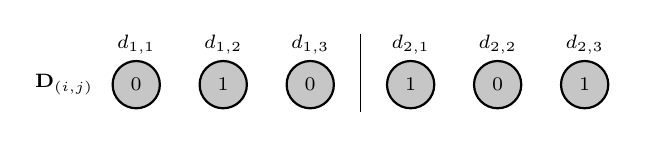
\begin{tikzpicture}[shorten >=1pt,->,draw=black!100, scale=0.85]
	\scriptsize
	\tikzstyle{label}=[text width=3em, text centered]
	\tikzstyle{annot}=[text width=2.5em]
	\tikzstyle{d-node}=[circle,draw=black!100,fill=gray!45,thick,inner sep=0pt,minimum size=6mm]
	
	\def \china{0.6cm}
	\def \data{0cm}
	
	\node[annot] (d-layer) at (0cm,\data) {$\mathbf{D}_{(i,j)}$};
	\draw[-] (4.45cm, \china+1.5mm) -- (4.45cm, \data-4.5mm);
%	\draw[-] (8.55cm, \china+1.5mm) -- (8.55cm, \data-4.5mm);
	%\draw[-] (-1cm, \china+.5cm) -- (13cm, \china+.5cm);
	%\draw[-] (-1cm, \data-.5cm) -- (13cm, \data-.5cm);
	
	\node[label] 	(dl00)	at (1.1cm,\china)		{$d_{1,1}$};
	\node[label] 	(dl01)	at (2.4cm,\china)		{$d_{1,2}$};
	\node[label] 	(dl02)	at (3.7cm,\china)	 	{$d_{1,3}$};
	
	\node[label] 	(dl10)	at (5.2cm,\china) 		{$d_{2,1}$};
	\node[label] 	(dl11) 	at (6.5cm,\china)   	{$d_{2,2}$};
	\node[label] 	(dl12)	at (7.8cm,\china)		{$d_{2,3}$};
	
	% \node[label] 	(dl20) 	at (9.3cm,\china)  		{$d_{3,1}$};
	% \node[label] 	(dl21)	at (10.6cm,\china) 		{$d_{3,2}$};
	% \node[label] 	(dl22) 	at (11.9cm,\china)   	{$d_{3,3}$};
	
	\node[d-node] 	(d00)	at (1.1cm,\data)		{$0$};
	\node[d-node] 	(d01)	at (2.4cm,\data)		{$1$};
	\node[d-node] 	(d02)	at (3.7cm,\data)		{$0$};

	\node[d-node] 	(d10)	at (5.2cm,\data)		{$1$};
	\node[d-node] 	(d11)	at (6.5cm,\data)		{$0$};
	\node[d-node] 	(d12)	at (7.8cm,\data)		{$1$};
	
	% \node[d-node] 	(d20)	at (9.3cm,\data)		{$1$};
	% \node[d-node] 	(d21)	at (10.6cm,\data)		{$1$};
	% \node[d-node] 	(d22)	at (11.9cm,\data)		{$1$};
\end{tikzpicture}
\label{fig:example:subfig0}
}
\end{center}

\usetikzlibrary{positioning}
%\begin{minipage}{.3\textwidth}
\begin{center}
\subfigure[Learning in Progress]{
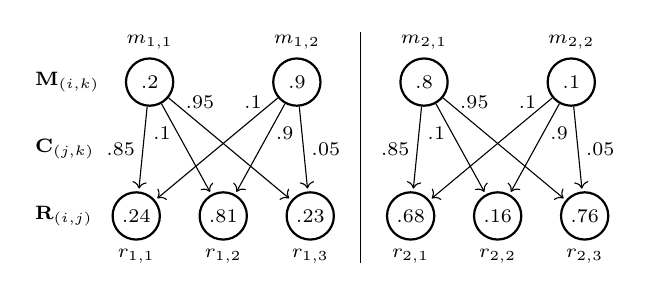
\begin{tikzpicture}[shorten >=1pt,->,draw=black!100, scale=0.85]
	\footnotesize
%	\def \attic{5.95cm}
%	\def \rowtwoht{5.4cm}
%	\def \weightlevel{3.9cm}
%	\def \rowoneht{2.4cm}
%	\def \basement{1.8cm}
%	\def \data{1cm}
%	\def \china{0cm}

	\def \attic{5cm}
	\def \rowtwoht{4.4cm}
	\def \weightlevel{3.4cm}
	\def \rowoneht{2.4cm}
	\def \basement{1.8cm}
	\def \data{1cm}
	\def \china{0cm}
		
	\tikzstyle{m-node}=[circle,draw=black!100,thick,inner sep=0pt,minimum size=6mm]
	\tikzstyle{r-node}=[circle,draw=black!100,thick,inner sep=0pt,minimum size=6mm]
	\tikzstyle{d-node}=[circle,draw=black!100,fill=gray!45,thick,inner sep=0pt,minimum size=6mm]
	%\tikzstyle{dots}=[text width=5ex, text centered]
	\tikzstyle{annot}=[text width=2.5em]
	% labels
	\tikzstyle{label}=[text width=2.5em, text centered]
	\tikzstyle{formula}=[text width=30em, text centered]
	
	\scriptsize
	\node[annot] (hidden-layer) at (0cm,\rowtwoht) {$\mathbf{M}_{(i,k)}$};
	\node[annot] (weights) at (0cm,\weightlevel) {$\mathbf{C}_{(j,k)}$};
	\node[annot] (r-layer) at (0cm,\rowoneht) {$\mathbf{R}_{(i,j)}$};
	
	% hidden layer
	\scriptsize
	\node[m-node] 	(ma00)	at (1.3cm,\rowtwoht)		{$.2$};
	\node[m-node] 	(ma01)	at (3.5cm,\rowtwoht)		{$.9$};
	\node[m-node] 	(ma10)	at (5.4cm,\rowtwoht) 	{$.8$};
	\node[m-node] 	(ma11)	at (7.6cm,\rowtwoht)	 	{$.1$};
	% \node[m-node] 	(m20)	at (9.65cm,\rowtwoht) 	{$.8$};
	% \node[m-node] 	(m21)	at (11.55cm,\rowtwoht)	 	{$.9$};
	
	%\footnotesize
	\node[label]	(ml00) 	at (1.3cm,\attic)		{$m_{1,1}$}; %1.75 -> 1.45
	\node[label]	(ml01) 	at (3.5cm,\attic)		{$m_{1,2}$}; %3.05 -> 3.35
	\node[label] 	(ml10)	at (5.4cm,\attic) 	{$m_{2,1}$};     %5.85 -> 5.55
	\node[label] 	(ml11)	at (7.6cm,\attic)	 	{$m_{2,2}$}; %7.15 -> 7.45
	% \node[label] 	(ml20)	at (9.65cm,\attic) 	{$m_{3,1}$};     %9.95 -> 9.65
	% \node[label] 	(ml21)	at (11.55cm,\attic)	 	{$m_{3,2}$}; %11.25 -> 11.55
	
	\scriptsize
	\node[r-node] 	(ra00)	at (1.1cm,\rowoneht)		{$.24$};
	\node[r-node] 	(ra01)	at (2.4cm,\rowoneht)		{$.81$};
	\node[r-node] 	(ra02)	at (3.7cm,\rowoneht)	 	{$.23$};
	
	\node[r-node] 	(ra10)	at (5.2cm,\rowoneht) 		{$.68$};
	\node[r-node] 	(ra11) 	at (6.5cm,\rowoneht)   	{$.16$};
	\node[r-node] 	(ra12)	at (7.8cm,\rowoneht)		{$.76$};
	
	\node[label] 	(rl00)	at (1.1cm,\basement)		{$r_{1,1}$};
	\node[label] 	(rl01)	at (2.4cm,\basement)		{$r_{1,2}$};
	\node[label] 	(rl02)	at (3.7cm,\basement)	 	{$r_{1,3}$};
	
	\node[label] 	(rl10)	at (5.2cm,\basement) 		{$r_{2,1}$};
	\node[label] 	(rl11) 	at (6.5cm,\basement)   	{$r_{2,2}$};
	\node[label] 	(rl12)	at (7.8cm,\basement)		{$r_{2,3}$};

	\draw[-] (4.45cm, \attic+1.5mm) -- (4.45cm, \basement-1.5mm);

	\scriptsize
	\path
		(ma00)	edge	node [left]	{$.85$} (ra00)
		(ma00)	edge	node [left,xshift=-1mm,yshift=2mm]	{$.1$}	(ra01)
		(ma00)	edge	node [left,xshift=-1mm,yshift=6mm]	{$.95$}	(ra02)

		(ma01)	edge	node [right,xshift=2.5mm,yshift=6mm]	{$.1$}	(ra00)
		(ma01)	edge	node [right,xshift=1mm,yshift=2mm]	{$.9$}	(ra01)
		(ma01)	edge	node [right]	{$.05$} (ra02)
		%
		(ma10)	edge	node [left] {$.85$} (ra10)
		(ma10)	edge	node [left,xshift=-1mm,yshift=2mm]	{$.1$}	(ra11)
		(ma10)	edge	node [left,xshift=-1mm,yshift=6mm] {$.95$}	(ra12)
		
		(ma11)	edge	node [right,xshift=2.5mm,yshift=6mm]	{$.1$}	(ra10)
		(ma11)	edge	node [right,xshift=1mm,yshift=2mm]	{$.9$}	(ra11)
		(ma11)	edge	node [right]	{$.05$} (ra12);
		%
		% (m20)	edge	node [left]	{$.85$}	(r20)
		% (m20)	edge	node [left,xshift=-1mm,yshift=4mm]	{$.1$}	(r21)
		% (m20)	edge	node [left,xshift=-1mm,yshift=10mm]	{$.95$} (r22)
		
		% (m21)	edge	node [right,xshift=3mm,yshift=10mm]		{$.1$}	(r20)
		% (m21)	edge	node [right,xshift=1mm,yshift=4mm]{$.9$}	(r21)
		% (m21)	edge	node [right]	{$.05$}	(r22);		
		
\end{tikzpicture}
\label{fig:example:subfig1}
}
\subfigure[Convergence]{

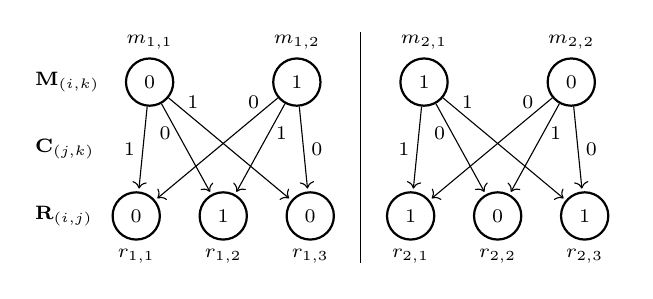
\begin{tikzpicture}[shorten >=1pt,->,draw=black!100, scale=0.85]
	\footnotesize
%	\def \attic{5.95cm}
%	\def \rowtwoht{5.4cm}
%	\def \weightlevel{3.9cm}
%	\def \rowoneht{2.4cm}
%	\def \basement{1.8cm}
%	\def \data{1cm}
%	\def \china{0cm}

%	\def \attic{5.2cm}
%	\def \rowtwoht{4.6cm}
%	\def \weightlevel{3.5cm}
%	\def \rowoneht{2.4cm}
%	\def \basement{1.8cm}
%	\def \data{1cm}
%	\def \china{0cm}

	\def \attic{5cm}
	\def \rowtwoht{4.4cm}
	\def \weightlevel{3.4cm}
	\def \rowoneht{2.4cm}
	\def \basement{1.8cm}
	\def \data{1cm}
	\def \china{0cm}
		
%	\def \attic{5.4cm}
%	\def \rowtwoht{5cm}
%	\def \weightlevel{3.9cm}
%	\def \rowoneht{2.4cm}
%	\def \basement{1.8cm}
%	\def \data{1cm}
%	\def \china{0cm}
	
	\scriptsize
	\tikzstyle{m-node}=[circle,draw=black!100,thick,inner sep=0pt,minimum size=6mm]
	\tikzstyle{r-node}=[circle,draw=black!100,thick,inner sep=0pt,minimum size=6mm]
	\tikzstyle{d-node}=[circle,draw=black!100,fill=gray!45,thick,inner sep=0pt,minimum size=6mm]
	\tikzstyle{annot}=[text width=2.5em]
	% labels
	\tikzstyle{label}=[text width=3em, text centered]
	\tikzstyle{formula}=[text width=30em, text centered]
	\node[annot] (hidden-layer) at (0cm,\rowtwoht) {$\mathbf{M}_{(i,k)}$};
	\node[annot] (weights) at (0cm,\weightlevel) {$\mathbf{C}_{(j,k)}$};
	\node[annot] (r-layer) at (0cm,\rowoneht) {$\mathbf{R}_{(i,j)}$};
	
	\node[m-node] 	(m00)	at (1.3cm,\rowtwoht)		{$0$};
	\node[m-node] 	(m01)	at (3.5cm,\rowtwoht)		{$1$};
	\node[m-node] 	(m10)	at (5.4cm,\rowtwoht) 	{$1$};
	\node[m-node] 	(m11)	at (7.6cm,\rowtwoht)	 	{$0$};
	% \node[m-node] 	(m20)	at (9.65cm,\rowtwoht) 	{$1$};
	% \node[m-node] 	(m21)	at (11.55cm,\rowtwoht)	 	{$1$};
	
	\node[label]	(ml00) 	at (1.3cm,\attic)		{$m_{1,1}$};
	\node[label]	(ml01) 	at (3.5cm,\attic)		{$m_{1,2}$};
	\node[label] 	(ml10)	at (5.4cm,\attic) 	{$m_{2,1}$};
	\node[label] 	(ml11)	at (7.6cm,\attic)	 	{$m_{2,2}$};
	% \node[label] 	(ml20)	at (9.65cm,\attic) 	{$m_{3,1}$};
	% \node[label] 	(ml21)	at (11.55cm,\attic)	 	{$m_{3,2}$};
	
	%\node[m-node] 	(m20)	[right of=m11,xshift=2cm]	 	{$1.0$};
	%\node[m-node] 	(m21)	[right of=m20,xshift=0.5cm]	 	{$1.0$};	
	% reconstructed vector
	\node[r-node] 	(r00)	at (1.1cm,\rowoneht)		{$0$};
	\node[label] 	(rl00)	at (1.1cm,\basement)		{$r_{1,1}$};
	\node[r-node] 	(r01)	at (2.4cm,\rowoneht)		{$1$};
	\node[label] 	(rl01)	at (2.4cm,\basement)		{$r_{1,2}$};
	\node[r-node] 	(r02)	at (3.7cm,\rowoneht)	 	{$0$};
	\node[label] 	(rl02)	at (3.7cm,\basement)	 	{$r_{1,3}$};
	
	\node[r-node] 	(r10)	at (5.2cm,\rowoneht) 		{$1$};
	\node[label] 	(rl10)	at (5.2cm,\basement) 		{$r_{2,1}$};
	\node[r-node] 	(r11) 	at (6.5cm,\rowoneht)   		{$0$};
	\node[label] 	(rl11) 	at (6.5cm,\basement)   		{$r_{2,2}$};
	\node[r-node] 	(r12)	at (7.8cm,\rowoneht)		{$1$};
	\node[label] 	(rl12)	at (7.8cm,\basement)		{$r_{2,3}$};
	
	% \node[r-node] 	(r20) 	at (9.3cm,\rowoneht)  		{$1$};
	% \node[label] 	(rl20) 	at (9.3cm,\basement)  		{$r_{3,1}$};
	% \node[r-node] 	(r21)	at (10.6cm,\rowoneht) 		{$1$};
	% \node[label] 	(rl21)	at (10.6cm,\basement) 		{$r_{3,2}$};
	% \node[r-node] 	(r22) 	at (11.9cm,\rowoneht)   		{$1$};
	% \node[label] 	(rl22) 	at (11.9cm,\basement)   		{$r_{3,3}$};
	
	\draw[-] (4.45cm, \attic+1.5mm) -- (4.45cm, \basement-1.5mm);
%	\draw[-] (8.55cm, \attic+1.5mm) -- (8.55cm, \basement-1.5mm);

	\path
		(m00)	edge	node [left] 	{$1$}	(r00)
		(m00)	edge	node [left,xshift=-1mm,yshift=2mm]	{$0$}	(r01)
		(m00)	edge	node [left,xshift=-3mm,yshift=6mm]	{$1$}	(r02)

		(m01)	edge	node [right,xshift=3mm,yshift=6mm]	{$0$}	(r00)
		(m01)	edge	node [right,xshift=1mm,yshift=2mm]	{$1$}	(r01)
		(m01)	edge	node [right]	{$0$}	(r02)
		%
		(m10)	edge	node [left] 	{$1$}	(r10)
		(m10)	edge	node [left,xshift=-1mm,yshift=2mm]	{$0$}	(r11)
		(m10)	edge	node [left,xshift=-3mm,yshift=6mm] {$1$}	(r12)
		
		(m11)	edge	node [right,xshift=3mm,yshift=6mm]	{$0$}	(r10)
		(m11)	edge	node [right,xshift=1mm,yshift=2mm]	{$1$}	(r11)
		(m11)	edge	node [right]	{$0$}	(r12);
		%
		% (m20)	edge	node [left]	{$1$}	(r20)
		% (m20)	edge	node [left,xshift=-1mm,yshift=4mm]	{$0$}	(r21)
		% (m20)	edge	node [left,xshift=-3mm,yshift=10mm]	{$1$} (r22)
		
		% (m21)	edge	node [right,xshift=3mm,yshift=10mm]		{$0$}	(r20)
		% (m21)	edge	node [right,xshift=1mm,yshift=4mm]{$1$}	(r21)
		% (m21)	edge	node [right]	{$0$}	(r22);		
\end{tikzpicture}
\label{fig:example:subfig2}
}

\begin{framed}
	\centering
	\small
	where
	$\begin{aligned}
	   r_{i,j} = 1 - \Pi_{k=1}^{K} (1 - m_{i,k}c_{j,k}) 
	\end{aligned}$
        \hspace{2em}
        [\textsc{noisy-or} function]
\end{framed}

\end{center}
\caption{A simple MCMM example} % showing learning in progress}
\label{fig:example}
\end{figure}

We can see that while learning is in progress, the cluster activities
($m_{i,k}$) and the cluster centers ($c_{j,k}$) are in flux, as the
error rate is being reduced, but that they converge to values of 0 and
1.  At convergence, a reconstruction node ($r_{i,j}$) is 1 if at least one
$m_{i,k}c_{j,k} = 1$ (and 0 otherwise).

%the activities and the centers are 1 and are 0 otherwise.

% \begin{figure*}[htb]
% \usetikzlibrary{positioning}
% \begin{center}
% \subfigure[Observed Data]{
% \begin{tikzpicture}[shorten >=1pt,->,draw=black!100]
% 	\scriptsize
% 	\tikzstyle{label}=[text width=3em, text centered]
% 	\tikzstyle{annot}=[text width=2.5em]
% 	\tikzstyle{d-node}=[circle,draw=black!100,fill=gray!45,thick,inner sep=0pt,minimum size=6mm]
	
% 	\def \china{0.6cm}
% 	\def \data{0cm}
	
% 	\node[annot] (d-layer) at (0cm,\data) {$\mathbf{D}_{(i,j)}$};
% 	\draw[-] (4.45cm, \china+1.5mm) -- (4.45cm, \data-4.5mm);
% 	\draw[-] (8.55cm, \china+1.5mm) -- (8.55cm, \data-4.5mm);
% 	%\draw[-] (-1cm, \china+.5cm) -- (13cm, \china+.5cm);
% 	%\draw[-] (-1cm, \data-.5cm) -- (13cm, \data-.5cm);
	
% 	\node[label] 	(dl00)	at (1.1cm,\china)		{$d_{1,1}$};
% 	\node[label] 	(dl01)	at (2.4cm,\china)		{$d_{1,2}$};
% 	\node[label] 	(dl02)	at (3.7cm,\china)	 	{$d_{1,3}$};
	
% 	\node[label] 	(dl10)	at (5.2cm,\china) 		{$d_{2,1}$};
% 	\node[label] 	(dl11) 	at (6.5cm,\china)   	{$d_{2,2}$};
% 	\node[label] 	(dl12)	at (7.8cm,\china)		{$d_{2,3}$};
	
% 	\node[label] 	(dl20) 	at (9.3cm,\china)  		{$d_{3,1}$};
% 	\node[label] 	(dl21)	at (10.6cm,\china) 		{$d_{3,2}$};
% 	\node[label] 	(dl22) 	at (11.9cm,\china)   	{$d_{3,3}$};
	
% 	\node[d-node] 	(d00)	at (1.1cm,\data)		{$0$};
% 	\node[d-node] 	(d01)	at (2.4cm,\data)		{$1$};
% 	\node[d-node] 	(d02)	at (3.7cm,\data)		{$0$};

% 	\node[d-node] 	(d10)	at (5.2cm,\data)		{$1$};
% 	\node[d-node] 	(d11)	at (6.5cm,\data)		{$0$};
% 	\node[d-node] 	(d12)	at (7.8cm,\data)		{$1$};
	
% 	\node[d-node] 	(d20)	at (9.3cm,\data)		{$1$};
% 	\node[d-node] 	(d21)	at (10.6cm,\data)		{$1$};
% 	\node[d-node] 	(d22)	at (11.9cm,\data)		{$1$};
% \end{tikzpicture}
% \label{fig:example:subfig0}
% }
% \end{center}

% \usetikzlibrary{positioning}
% %\begin{minipage}{.3\textwidth}
% \begin{center}
% \subfigure[Learning in Progress]{
% \begin{tikzpicture}[shorten >=1pt,->,draw=black!100]
% 	\footnotesize
% 	\def \attic{5.95cm}
% 	\def \rowtwoht{5.4cm}
% 	\def \weightlevel{3.9cm}
% 	\def \rowoneht{2.4cm}
% 	\def \basement{1.8cm}
% 	\def \data{1cm}
% 	\def \china{0cm}
	
% 	\tikzstyle{m-node}=[circle,draw=black!100,thick,inner sep=0pt,minimum size=6mm]
% 	\tikzstyle{r-node}=[circle,draw=black!100,thick,inner sep=0pt,minimum size=6mm]
% 	\tikzstyle{d-node}=[circle,draw=black!100,fill=gray!45,thick,inner sep=0pt,minimum size=6mm]
% 	%\tikzstyle{dots}=[text width=5ex, text centered]
% 	\tikzstyle{annot}=[text width=2.5em]
% 	% labels
% 	\tikzstyle{label}=[text width=3em, text centered]
% 	\tikzstyle{formula}=[text width=30em, text centered]
	
% 	\scriptsize
% 	\node[annot] (hidden-layer) at (0cm,\rowtwoht) {$\mathbf{M}_{(i,k)}$};
% 	\node[annot] (weights) at (0cm,\weightlevel) {$\mathbf{C}_{(j,k)}$};
% 	\node[annot] (r-layer) at (0cm,\rowoneht) {$\mathbf{R}_{(i,j)}$};
	
% 	% hidden layer
% 	\scriptsize
% 	\node[m-node] 	(m00)	at (1.45cm,\rowtwoht)		{$.2$};
% 	\node[m-node] 	(m01)	at (3.35cm,\rowtwoht)		{$.9$};
% 	\node[m-node] 	(m10)	at (5.55cm,\rowtwoht) 	{$.8$};
% 	\node[m-node] 	(m11)	at (7.45cm,\rowtwoht)	 	{$.1$};
% 	\node[m-node] 	(m20)	at (9.65cm,\rowtwoht) 	{$.8$};
% 	\node[m-node] 	(m21)	at (11.55cm,\rowtwoht)	 	{$.9$};
	
% 	%\footnotesize
% 	\node[label]	(ml00) 	at (1.45cm,\attic)		{$m_{1,1}$}; %1.75 -> 1.45
% 	\node[label]	(ml01) 	at (3.35cm,\attic)		{$m_{1,2}$}; %3.05 -> 3.35
% 	\node[label] 	(ml10)	at (5.55cm,\attic) 	{$m_{2,1}$};     %5.85 -> 5.55
% 	\node[label] 	(ml11)	at (7.45cm,\attic)	 	{$m_{2,2}$}; %7.15 -> 7.45
% 	\node[label] 	(ml20)	at (9.65cm,\attic) 	{$m_{3,1}$};     %9.95 -> 9.65
% 	\node[label] 	(ml21)	at (11.55cm,\attic)	 	{$m_{3,2}$}; %11.25 -> 11.55
	
% 	\scriptsize
% 	\node[r-node] 	(r00)	at (1.1cm,\rowoneht)		{$.24$};
% 	\node[r-node] 	(r01)	at (2.4cm,\rowoneht)		{$.81$};
% 	\node[r-node] 	(r02)	at (3.7cm,\rowoneht)	 	{$.23$};
	
% 	\node[r-node] 	(r10)	at (5.2cm,\rowoneht) 		{$.68$};
% 	\node[r-node] 	(r11) 	at (6.5cm,\rowoneht)   	{$.16$};
% 	\node[r-node] 	(r12)	at (7.8cm,\rowoneht)		{$.76$};
	
% 	\node[r-node] 	(r20) 	at (9.3cm,\rowoneht)  		{$.71$};
% 	\node[r-node] 	(r21)	at (10.6cm,\rowoneht) 		{$.83$};
% 	\node[r-node] 	(r22) 	at (11.9cm,\rowoneht)   	{$.77$};
	
% 	\node[label] 	(rl00)	at (1.1cm,\basement)		{$r_{1,1}$};
% 	\node[label] 	(rl01)	at (2.4cm,\basement)		{$r_{1,2}$};
% 	\node[label] 	(rl02)	at (3.7cm,\basement)	 	{$r_{1,3}$};
	
% 	\node[label] 	(rl10)	at (5.2cm,\basement) 		{$r_{2,1}$};
% 	\node[label] 	(rl11) 	at (6.5cm,\basement)   	{$r_{2,2}$};
% 	\node[label] 	(rl12)	at (7.8cm,\basement)		{$r_{2,3}$};
	
% 	\node[label] 	(rl20) 	at (9.3cm,\basement)  		{$r_{3,1}$};
% 	\node[label] 	(rl21)	at (10.6cm,\basement) 		{$r_{3,2}$};
% 	\node[label] 	(rl22) 	at (11.9cm,\basement)   	{$r_{3,3}$};

% 	\draw[-] (4.45cm, \attic+1.5mm) -- (4.45cm, \basement-1.5mm);
% 	\draw[-] (8.55cm, \attic+1.5mm) -- (8.55cm, \basement-1.5mm);

% 	\scriptsize
% 	\path
% 		(m00)	edge	node [left] 	{$.85$}	(r00)
% 		(m00)	edge	node [left,xshift=-1mm,yshift=4mm]	{$.1$}	(r01)
% 		(m00)	edge	node [left,xshift=-1mm,yshift=10mm]	{$.95$}	(r02)

% 		(m01)	edge	node [right,xshift=3mm,yshift=10mm]	{$.1$}	(r00)
% 		(m01)	edge	node [right,xshift=1mm,yshift=4mm]	{$.9$}	(r01)
% 		(m01)	edge	node [right]	{$.05$}	(r02)
% 		%
% 		(m10)	edge	node [left] 	{$.85$}	(r10)
% 		(m10)	edge	node [left,xshift=-1mm,yshift=4mm]	{$.1$}	(r11)
% 		(m10)	edge	node [left,xshift=-1mm,yshift=10mm] {$.95$}	(r12)
		
% 		(m11)	edge	node [right,xshift=3mm,yshift=10mm]	{$.1$}	(r10)
% 		(m11)	edge	node [right,xshift=1mm,yshift=4mm]	{$.9$}	(r11)
% 		(m11)	edge	node [right]	{$.05$}	(r12)
% 		%
% 		(m20)	edge	node [left]	{$.85$}	(r20)
% 		(m20)	edge	node [left,xshift=-1mm,yshift=4mm]	{$.1$}	(r21)
% 		(m20)	edge	node [left,xshift=-1mm,yshift=10mm]	{$.95$} (r22)
		
% 		(m21)	edge	node [right,xshift=3mm,yshift=10mm]		{$.1$}	(r20)
% 		(m21)	edge	node [right,xshift=1mm,yshift=4mm]{$.9$}	(r21)
% 		(m21)	edge	node [right]	{$.05$}	(r22);		
		
% \end{tikzpicture}
% \label{fig:example:subfig1}
% }
% \subfigure[Convergence]{

% \begin{tikzpicture}[shorten >=1pt,->,draw=black!100]
% 	\footnotesize
% 	\def \attic{5.95cm}
% 	\def \rowtwoht{5.4cm}
% 	\def \weightlevel{3.9cm}
% 	\def \rowoneht{2.4cm}
% 	\def \basement{1.8cm}
% 	\def \data{1cm}
% 	\def \china{0cm}
	
% 	\scriptsize
% 	\tikzstyle{m-node}=[circle,draw=black!100,thick,inner sep=0pt,minimum size=6mm]
% 	\tikzstyle{r-node}=[circle,draw=black!100,thick,inner sep=0pt,minimum size=6mm]
% 	\tikzstyle{d-node}=[circle,draw=black!100,fill=gray!45,thick,inner sep=0pt,minimum size=6mm]
% 	\tikzstyle{annot}=[text width=2.5em]
% 	% labels
% 	\tikzstyle{label}=[text width=3em, text centered]
% 	\tikzstyle{formula}=[text width=30em, text centered]
% 	\node[annot] (hidden-layer) at (0cm,\rowtwoht) {$\mathbf{M}_{(i,k)}$};
% 	\node[annot] (weights) at (0cm,\weightlevel) {$\mathbf{C}_{(j,k)}$};
% 	\node[annot] (r-layer) at (0cm,\rowoneht) {$\mathbf{R}_{(i,j)}$};
	
% 	\node[m-node] 	(m00)	at (1.45cm,\rowtwoht)		{$0$};
% 	\node[m-node] 	(m01)	at (3.35cm,\rowtwoht)		{$1$};
% 	\node[m-node] 	(m10)	at (5.55cm,\rowtwoht) 	{$1$};
% 	\node[m-node] 	(m11)	at (7.45cm,\rowtwoht)	 	{$0$};
% 	\node[m-node] 	(m20)	at (9.65cm,\rowtwoht) 	{$1$};
% 	\node[m-node] 	(m21)	at (11.55cm,\rowtwoht)	 	{$1$};
	
% 	\node[label]	(ml00) 	at (1.45cm,\attic)		{$m_{1,1}$};
% 	\node[label]	(ml01) 	at (3.35cm,\attic)		{$m_{1,2}$};
% 	\node[label] 	(ml10)	at (5.55cm,\attic) 	{$m_{2,1}$};
% 	\node[label] 	(ml11)	at (7.45cm,\attic)	 	{$m_{2,2}$};
% 	\node[label] 	(ml20)	at (9.65cm,\attic) 	{$m_{3,1}$};
% 	\node[label] 	(ml21)	at (11.55cm,\attic)	 	{$m_{3,2}$};
	
% 	%\node[m-node] 	(m20)	[right of=m11,xshift=2cm]	 	{$1.0$};
% 	%\node[m-node] 	(m21)	[right of=m20,xshift=0.5cm]	 	{$1.0$};	
% 	% reconstructed vector
% 	\node[r-node] 	(r00)	at (1.1cm,\rowoneht)		{$0$};
% 	\node[label] 	(rl00)	at (1.1cm,\basement)		{$r_{1,1}$};
% 	\node[r-node] 	(r01)	at (2.4cm,\rowoneht)		{$1$};
% 	\node[label] 	(rl01)	at (2.4cm,\basement)		{$r_{1,2}$};
% 	\node[r-node] 	(r02)	at (3.7cm,\rowoneht)	 	{$0$};
% 	\node[label] 	(rl02)	at (3.7cm,\basement)	 	{$r_{1,3}$};
	
% 	\node[r-node] 	(r10)	at (5.2cm,\rowoneht) 		{$1$};
% 	\node[label] 	(rl10)	at (5.2cm,\basement) 		{$r_{2,1}$};
% 	\node[r-node] 	(r11) 	at (6.5cm,\rowoneht)   		{$0$};
% 	\node[label] 	(rl11) 	at (6.5cm,\basement)   		{$r_{2,2}$};
% 	\node[r-node] 	(r12)	at (7.8cm,\rowoneht)		{$1$};
% 	\node[label] 	(rl12)	at (7.8cm,\basement)		{$r_{2,3}$};
	
% 	\node[r-node] 	(r20) 	at (9.3cm,\rowoneht)  		{$1$};
% 	\node[label] 	(rl20) 	at (9.3cm,\basement)  		{$r_{3,1}$};
% 	\node[r-node] 	(r21)	at (10.6cm,\rowoneht) 		{$1$};
% 	\node[label] 	(rl21)	at (10.6cm,\basement) 		{$r_{3,2}$};
% 	\node[r-node] 	(r22) 	at (11.9cm,\rowoneht)   		{$1$};
% 	\node[label] 	(rl22) 	at (11.9cm,\basement)   		{$r_{3,3}$};
	
% 	\draw[-] (4.45cm, \attic+1.5mm) -- (4.45cm, \basement-1.5mm);
% 	\draw[-] (8.55cm, \attic+1.5mm) -- (8.55cm, \basement-1.5mm);

% 	\path
% 		(m00)	edge	node [left] 	{$1$}	(r00)
% 		(m00)	edge	node [left,xshift=-1mm,yshift=4mm]	{$0$}	(r01)
% 		(m00)	edge	node [left,xshift=-3mm,yshift=10mm]	{$1$}	(r02)

% 		(m01)	edge	node [right,xshift=3mm,yshift=10mm]	{$0$}	(r00)
% 		(m01)	edge	node [right,xshift=1mm,yshift=4mm]	{$1$}	(r01)
% 		(m01)	edge	node [right]	{$0$}	(r02)
% 		%
% 		(m10)	edge	node [left] 	{$1$}	(r10)
% 		(m10)	edge	node [left,xshift=-1mm,yshift=4mm]	{$0$}	(r11)
% 		(m10)	edge	node [left,xshift=-3mm,yshift=10mm] {$1$}	(r12)
		
% 		(m11)	edge	node [right,xshift=3mm,yshift=10mm]	{$0$}	(r10)
% 		(m11)	edge	node [right,xshift=1mm,yshift=4mm]	{$1$}	(r11)
% 		(m11)	edge	node [right]	{$0$}	(r12)
% 		%
% 		(m20)	edge	node [left]	{$1$}	(r20)
% 		(m20)	edge	node [left,xshift=-1mm,yshift=4mm]	{$0$}	(r21)
% 		(m20)	edge	node [left,xshift=-3mm,yshift=10mm]	{$1$} (r22)
		
% 		(m21)	edge	node [right,xshift=3mm,yshift=10mm]		{$0$}	(r20)
% 		(m21)	edge	node [right,xshift=1mm,yshift=4mm]{$1$}	(r21)
% 		(m21)	edge	node [right]	{$0$}	(r22);		
% \end{tikzpicture}
% \label{fig:example:subfig2}
% }

% \begin{framed}
% 	\centering
% 	\small
% 	where
% 	$\begin{aligned}
% 	   r_{i,j} = 1 - \Pi_{k=1}^{K} (1 - m_{i,k}c_{j,k}) 
% 	\end{aligned}$
% \end{framed}

% \label{fig:example}
% \caption{MCMM example showing learning in progress}
% \end{center}
% \end{figure*}

 % The MCMM
\chapter{Autonomous Morphology as a Target of Learning}
\label{autonomous}

\section{Introduction}
Many morphologists in recent decades have rejected the notion of the morpheme---a concept that inextricably binds morphology to syntax and semantics---in favor of approaches that regard morphology as autonomous, i.e., as independent 
of both syntax/semantics and phonology. The principle objective of this chapter is to 
show that autonomous morphological units are legitimate learning targets for system of unsupervised morphological learning. In fact, as we will soon see, autonomous morphology is more than just legitimate; it is the only possible learning target for the unsupervised learning of morphology (ULM) as it is conventionally defined.
In the course of the discussion, we shall consider some of the more prominent theories of autonomous morphology, contrasting them with ``non-automonous'' approaches, and  noting their significance to ULM (and Multimorph in particular).


\section{The Unsupervised Learning of \textit{What}, Exactly?}
\label{sec:what-exactly}
In the ULM literature, authors often use the word \emph{morpheme(s)} 
when describing their systems' \emph{learning target(s)}, i.e., what their systems are meant to learn and 
output, as well as the features that compose their input feature vectors.
\cite{poon-et-al:2009}, for example, use two main categories 
of features, one of which they refer to as \emph{morpheme-context} features (see chapter \ref{ch:lit-review}).
\cite{goldsmith:2001, goldsmith:2006} also uses the word 
\emph{morpheme}.
The creators of Morfessor 
\citep{creutz-and-lagus:2002, 
creutz-and-lagus:2005, creutz-and-lagus:2007}
use a range of terms, including 
\emph{morpheme},
\emph{morpheme-like}, and \emph{morph}. The following quotations 
illustrate these usages (emphasis added):
\begin{exe}
\ex ``The model presented in this 
work provides a good means for the segmentation of words into 
\textbf{morphemes} \citep[][p. 6]{creutz-and-lagus:2007}. 
\ex``[W]e have demonstrated how the meaning and form of 
\textbf{morpheme-like} units can be modeled in a 
morphology induction task\dots'' \citep{creutz-and-lagus:2005}.
\ex``The lexicon contains one entry for each distinct \textbf{morph} 
(morph type) in the 
segmented corpus'' \citep[][p. 9]{creutz-and-lagus:2007}. 
\end{exe}
Creutz and Lagus seem to prefer the more general, theory-neutral term \emph{morph} 
in more formal or technical contexts. Indeed,
of the above three terms, they probably use 
\emph{morph} most frequently.

Moreover, ULM researchers virtually never specify what they mean
when they use the word \emph{morphology}, even though there
are currently at least two fundamentally different schools of thought concerning the nature of morphology. These are the 
the \emph{morpheme-based} and \emph{lexeme-based} views, to borrow the labels that \cite{aronoff:1994} has assigned 
to these categories. The lexeme-based view, which has been gaining momentum in recent decades \citep{anderson:2017},
is that there exists an \emph{autonomous} layer of morphology, a layer that mediates between (morpho-)syntax
and phonological realization, but has neither meaning nor phonologically realized form in and of itself. Proponents
of lexeme-based morphology thus do not believe in pairings of form and meaning, i.e., \emph{morphemes}, as fundamental linguistic
units \citep{anderson:2015}. We will further discuss the notion of autonomous morphology in section~\ref{sec:morpho-theories}.

One's morphological theory affects the way in which one interprets the output of a ULM  system. 
If one describes a ULM  system and its learning task in terms of 
morpheme-based morphology, one must also struggle to 
describe its output as consisting of morphemes, as do, for example, 
\cite{creutz-and-lagus:2007,creutz-and-lagus:2005}. In contrast, under a 
lexeme-based theory, one would view the output of a ULM  system as 
consisting of \emph{autonomous} morphological units, i.e., 
expressly non-morpheme units. 
Thus, one's theory of morphology makes an implicit claim about the output of 
his/her ULM  system.

The output of any machine learning system depends to 
a great extent on the nature of its input, which, in the case of the 
\emph{unsupervised} learning of morphology, 
depends to a large extent on with the meaning of ``unsupervised.'' 
All of the major ULM  
systems take as input a list of independent tokenized words 
\citep[e.g.,][]{goldsmith:2001,baroni-et-al:2002,creutz-and-lagus:2005,poon-et-al:2009}
Thus, a convention seems to have emerged whereby, in the 
case of ULM , the meaning of \emph{unsupervised} includes a
requirement that each word be free of morphosyntactic 
or semantic information. In practice,
this means being entirely free of context. I am 
not aware of a ULM system that extracts features from the raw context surrounding a given word, i.e.,
the unanalyzed words adjacent to the unanalyzed word question. It seems doubtful
that such a context could be helpful to a machine learner. 
It would probably have to be abstracted and categorized 
(i.e., annotated) in order
for it to be helpful to a system.

%Because morphemes are irreducible and arbitrary pairings of form and meaning
%but in 
Classical morphemes are (irreducible) pairings of form and meaning.
In order to learn morphemes, therefore, a system needs to learn meaning. But a ULM system does not have access to
the contexts of its input words, as its input is a list of independent word tokens, and thus it cannot learn
meaning.
% because the input to ULM systems is a list of contextless tokenized words. 
% learning meaning without contextual information. And since the input to a ULM 
% a ULM system consists of independent words without contextdoes not have access to context, it simply 
cannot learn classical morphemes. 
A ULM system might learn 
character subsequences that happen to resemble
 classical morphemes \emph{in form}, but only because morphological systems
do tend to cooperate with syntax/semantics in some way, and in some 
 cases this cooperation is more transparent and straightforward than
 in others.  However, this ULM system would nevertheless be oblivious to the actual meanings
 of these pieces of form. Meaning is an essential component of the classical morpheme, and because
 meaning depends on context, there is no way to induce classical morphemes from contextless words.
Therefore, ULM systems, particularly those which learn solely from 
from lists of raw, contextless words, simply cannot learn 
\emph{morphemes} in the strict sense of the term.

Consider, for example, Linguistica, the seminal 
ULM  system developed by \cite{goldsmith:2001, goldsmith:2006}. 
Linguistica finds morphological relationships by filling in 
data structures 
called \emph{signatures} as it iterates over datasets comprising many
thousands of contextless words. Each signature $\sigma$ 
comprises 
two sets, $S$ and $A$, a set of stems and a set of affixes, 
respectively.
A \emph{signature} is a pair of sets, namely a set of stems $S$ and 
a set of affixes $A$, such that each stem-affix combination in the cross 
product $S \times A$ is observed in the corpus. Additionally, $S$ and 
$A$ must each contain at least two members, with \textsc{null} being 
a permissible member, and each stem can belong to only one signature.  
For example, a signature could be the following: $S = \{ \text{act}, \text{back}, \text{mint} \}$ 
and $A = \{ \textsc{null}, \text{s}\}$. Every possible stem-affix combination is 
\begin{equation}
\label{eq:SxA}
S \times A = \{ \text{act}, \text{back}, \text{mint}, \text{act-s}, 
\text{back-s}, \text{mint-s}\}
\end{equation}
The fifth 
most common signature that Linguistica found among the words of 
\textit{Tom Sawyer} had as its affix set $\{\textsc{null}\textit{.ed.ing.s}\}$ \citep{goldsmith:2001}. 
The corresponding stem set had 14 members, though \citet{goldsmith:2001} 
does not identify the individual stems. 
In any case, the affix set \textsc{null}\textit{.ed.ing.s} represents 
a stem equivalence class. Its extraction would be an impressive achievement for any ULM system, and this
is but one of many such signatures that Linguistica has found. However, 
suppose we had no knowledge of English. It would then be impossible to deduce the nature 
of this equivalence class. We might
guess that it is a morphosyntactic category of \emph{some kind}, but since we would be ignorant
of the affixes' meanings/functions, this would be nothing more than a guess. 

An English speaker can probably deduce that \textsc{null}\textit{.ed.ing.s} are suffixes that attach to verbs,
but this it is the speaker's general competence in the language that informs this deduction, not anything in the 
signatures themselves.

Thus, although Linguistica does learn morphological equivalence classes, 
sets of stems that combine with the same affixes 
(and sets of affixes that combine with with the same stems) 
it does not learn to associate \textit{-s}, for example, 
with `3rd-person singular present-tense'. That is, it does not assign particular
meanings to the stems and affixes it discovers.
Nor would Linguistica know the particular meaning of any stem 
associated with a given affix set. 
Suppose that \{\textit{act}, \emph{jump}, \emph{laugh}\} 
was the stem set associated with \textsc{null}\textit{.ed.ing.s}. 
Linguistica would thus have learned that these stems are the same 
in a way. But Linguistica would not have learned what this 
equivalence should have signified, not would have learned the semantic 
distinctions between the members of the same equivalence set. 
That is, even though \textit{act}, \emph{jump}, and \emph{laugh} 
share the same affix set, they do not share the same meaning. 
Thus, we must conclude that Linguistica does not learn morphemes 
in the classical sense, i.e., with each morpheme being a
pairing of one form and one meaning.

To be sure, this is not a failing on the 
part of Linguistica, which is indeed an effective 
unsupervised learner of morphology. Given the definition 
of the classical morpheme and the limited nature of 
Linguistica's input, it is simply not possible for 
Linguistica to learn true morphemes. First, because 
Linguistica is an \emph{unsupervised} learner, it has 
no access to the information it would need to assign meaning to units of form.
Second, as we will see in section~\ref{sec:morpho-theories}, morphemes do not adequately 
account for the full range of morphological phenomena \citep{anderson:2017}. 
For these reasons, morphemes are not reasonable 
targets of unsupervised morphological learning.

\section{A Spectrum of Morphological Theories}
\label{sec:morpho-theories}
In the preceding section, we argued that Linguistica does not learn morphemes. The same can be said of Morfessor, 
the system of \cite{poon-et-al:2009}, and
every other ULM  system.
 But how can we say that these systems learn morphology, but not morphemes? As it turns out,
 the existence of morphemes is by no means a sure thing.  

\subsection{Stump's Taxonomy of Morphological Theories}
\cite{stump:2001}'s oft-cited taxonomy of morphological theories 
consists of four categories. These four arise from two independent 
binary distinctions, namely \emph{lexical} vs. \emph{inferential} on the hand, and \emph{incremental} vs. \emph{realizational} on the other.
 
\begin{exe}
\ex \textsc{First Distinction}: \textit{Lexical vs. Inferential} 
\begin{xlist}
	\ex \textbf{Lexical}: \textit{A word's meaning is the compositions of its components' lexical entries.}\\
	The meaning of \textit{issue-s}, for example, is determined by the lexical entries of its components \textit{issue} and \textit{-s}.
	\ex \textbf{Inferential}: \textit{A word's meaning is determined by the meanings of related words.}\\
	The meaning of \textit{issue-s} is determined by the meanings of related forms like \textit{dog-s} and \textit{bike-s},
with ``similarities of form [directly] reflecting similarities of content and vice versa'' \citep[][p. 2]{anderson:2015shorthist}. \label{ex:d-one-b}
	\end{xlist}
\ex \textsc{Second Distinction}: \textit{Incremental vs. Realizational} 
\begin{xlist} 
	\ex \textbf{Incremental}: Each affix has its own intrinsic meaning. 
	A form's morphosyntactic property set is thus built up incrementally as it acquires affixes.
	\label{ex:d-two-a}
	\ex \textbf{Realizational}: A word's set of morphosyntactic properties 
	licenses a particular configuration of morphological exponents 
	(i.e., usually affixes of some sort). 
	\end{xlist}
\end{exe}

By cross-combining the options of first distinction with those of the second, 
\cite{stump:2001} derives four categories of morphological theories. 
\emph{Lexical-Incremental} and \emph{Lexical-Realizational} theories 
on the one hand, and on the other, \emph{Inferential-Incremental} and 
\emph{Inferential-Realizational} theories. However, \citet{anderson:2017} 
notes that most theories fall into the \emph{Lexical-Incremental} and 
\emph{Inferential-Realizational} categories. Indeed, these are the two are 
the most extreme of the four categories in that they are entirely antithetical. 
The ongoing debate over the nature and status of morphology can largely 
be framed in terms of the opposition between these two categories. 

The distinction between \emph{Lexical-Incremental} 
and \emph{Lexical-Realizational} 
theories is essentially the same as the distinction 
that \cite{aronoff:1994} draws
between \emph{morpheme-based} and \emph{lexeme-based} 
views of morphology. Morpheme-based approaches regard 
the classical morpheme as the seat of meaning.
The concept of the morpheme and morpheme-centered morphological analysis
was developed by Bloomfield in the 1920s and 1930s by
\citet{bloomfield:1926, bloomfield:1933} and honed by his 
successors in the descriptivist program, e.g., 
\cite{hockett:1947} and \cite{harris:1955}.
It was \citet[][p. 161]{bloomfield:1933} who famously wrote, ``A linguistic form 
which bears no partial phonetic-semantic resemblance to any other form is a \emph{simple} form or \emph{morpheme}'' (emphasis in the original). 
That is, a morpheme, as a pairing of a form and a meaning, is a fundamental unit; it cannot be analyzed into smaller units
of form and meaning.
Moreover, Bloomfield and the descriptivists maintained that
each \emph{complex form}, i.e., each word comprising 
two or more morphemes, was \emph{exhaustively decomposable} 
into morphemes. That is, every phonological segment
in a given word had to be either a morpheme or part of a morpheme. 

The influence of Bloomfield and the descriptivists
cannot be easily underestimated. Bloomfieldian concepts and methods 
pervade introductory linguistics courses and textbooks, both at
the undergraduate and graduate level. Any introductory text containing 
a unit on morphological analysis is going to present a methodology that 
is essentially Bloomfieldian \citep{anderson:2017}.
It is therefore perhaps no surprise that
computational linguists, including researchers in the field of ULM, 
tend to presume
the reality of Bloomfieldian morphemes and the soundness of a 
Bloomfieldian view of morphology. The Bloomfieldian approach is essentially
the lexical-incremental approach.

By contrast, lexeme-based approaches (also called \emph{word-based} 
approaches) consider the seat of meaning to be the whole word rather than its components. According to this view, the component 
parts of a complex word do not have their own predetermined meanings. 
Rather, 
there is a buffer layer between the level of phonological form and the level of
syntax/semantics. This
buffer consists of morphological rules that map from raw phonological 
strings to meanings.
Paridigm Function Morphology, a lexeme-based theory developed by \citet{stump:2001}, 
posits a morphological architecture consisting of two kinds of paradigms: a \emph{content} paradigm and a \emph{form} paradigm.
The cells of the content paradigm are related to those of the form paradigm via
\emph{paradigm functions}.
A paradigm function follows the template
%\eqref{eq:PF}, 
\begin{equation}
\label{eq:PF}
	\text{PF}\langle \text{L},\sigma \rangle = \langle \text{X}, \sigma^\prime \rangle
\end{equation}
where the lefthand side represents a particular cell in the 
content paradigm, and the righthand side a particular form-paradigm cell.
In particular, $\text{L}$ is a lexeme, and $\text{X}$ is a stem, that is, the form correspondent of $\text{L}$. 
The morphosyntactic property set associated with content cell and form cell are $\sigma$ and 
$\sigma\prime$, respectively. In the canonical case, there is a one-to-one
correspondence between content cells and paradigm cells, and 
$\sigma = \sigma^\prime$.
Often, however, the mapping between content and form cells is 
not one-to-one, $\sigma \ne \sigma^\prime$, such as in cases of
\emph{syncretism}, wherein the mapping from content to form cells is many to one. 
Consider, for example, table 
\ref{tab:engverbpres}, which shows both the content and form paradigms 
for the English lexeme \emph{kick} in the simple present tense.
The content paradigm has six cells, one for each combination of \textsc{person} 
and \textsc{number}, while the form paradigm has only two, one for the 
form that has no suffix (\textit{kick}) and the other for the form 
that ends in \textit{-s}, namely \textit{kicks}. 
 
\begin{table}[t]
\setlength{\extrarowheight}{6pt}
\centering
\begin{tabular}{ccc}
\toprule
Content Paradigm & Form Paradigm & Realization \\% inserts table
\midrule %heading
$\langle \textsc{kick}, \{ \textsc{p:1}, \textsc{n:}\text{sg} \}\rangle $ & \multirow{5}{*}{\raisebox{-32pt}{$\Bigg\langle \textsc{kick}, 
\Big\{ \big((\textsc{p:}\text{1}\vee\text{2}) \land (\textsc{n:}\text{sg} \vee \text{pl})\big) 
\vee (\textsc{p:}\text{3}\land \textsc{n:}\text{pl}) \Big\} \Bigg\rangle$}} 
& \multirow{5}{*}{\raisebox{-20pt}{kick}} \\ \cmidrule{1-1}
$\langle \textsc{kick},\{\textsc{p:2}, \textsc{n:}\text{sg}\}\rangle$  &\\ \cmidrule{1-1}
$\langle \textsc{kick}, \{\textsc{p:1}, \textsc{n:}\text{pl}\}\rangle$  & \\ \cmidrule{1-1}
$\langle \textsc{kick}, \{\textsc{p:2}, \textsc{n:}\text{pl}\}\rangle$ &  \\ \cmidrule{1-1}
$\langle \textsc{kick}, \{\textsc{p:3}, \textsc{n:}\text{pl}\}\rangle$ & \\ \midrule
$\langle \textsc{kick}, \{\textsc{p:3}, \textsc{n:}\text{sg}\} \rangle$ & $\langle\textsc{kick}, \{\textsc{p:3}, \textsc{n:}\text{sg}\}\rangle$  & kicks \\
\bottomrule
\end{tabular}
\caption{Dual-paradigm analysis of the English present tense}
\label{tab:engverbpres}
\end{table}

Notice the unnaturalness of the two morphosyntactic classes in
the form-paradigm column in table \ref{tab:engverbpres}.
Classes like these abound in morphology.  
They are unnatural in that they are not motivated by morphosyntactic properties. Thus, from a morphosyntactic
perspective, they are quite arbitrary.
There is no reason to put the third-person singular alone in one class and all of the other combinations, 
including the other singular categories as well as third-person plural, together in the other class. Such classes help motivate 
a theory of an \emph{autonomous} layer of morphology, that is, a layer responsible 
for mapping from the content level to the phonological, but does so according 
to its own terms.

Surface forms are realized phonologically by \emph{realizational rules}, which 
are functions that map from form cells (for example, those in the second column in table~\ref{tab:engverbpres})
to fully realized phonological forms (the third column in table~\ref{tab:engverbpres}). 
In fact, each realizational rule is a bijection: Every 
distinct phonological form implies the existence of a unique corresponding cell in 
the form paradigm, and conversely, each distinct form cell implies the existence of 
a distinct corresponding phonological form. The
content-paradigm cells are not directly connected to the realizational rules of 
the phonological level because the form paradigm acts as an 
intervening layer---a layer of autonomous morphology---between the 
content paradigm and the level of phonological realization. 
Thus, according to Paradigm Function Morphology, the content paradigm cannot directly influence phonological form. 

Realizational rules come in two varieties:
\emph{rules of exponence} and \emph{rules of referral}. Rules of exponence, as exemplified in \eqref{eq:roexp}, describe the 
realization of surface forms from morphological \emph{exponents}. They take the form 
$\text{X},\text{C},\sigma \to f(\text{X})$, where X is the stem, C is the lexical category of X, 
$\sigma$ is a morphosyntactic property set,  and $f(\text{X})$ is the morphological operation to be performed 
on X, as in ``Xs'' (addition of an \emph{-s} suffix). The two rules of exponence in \eqref{eq:roexp}  
correspond to the two forms 
of English present-tense verbs (see table~\ref{tab:engverbpres}). 
\begin{align}
\label{eq:roexp}
	\text{X},\text{V},\sigma\text{:} \quad
	\{ \textsc{pers:3}\text{,} \land \textsc{num:}\text{sg,} \land \textsc{tns:}\text{pres} \} &= \text{X}s \\ 
	%\label{eq:roexp1}
	\text{X},\text{V},\tau\text{:} \quad
	%\{((\textsc{pers:}\text{1}\vee\text{2}) \land (\textsc{num:}\text{sg}\vee\text{pl})) \vee (\textsc{pers:}3 \vee \text{sg})\} 
	%\Bigg\langle \textsc{kick}, 
\Big\{ \big((\textsc{pers:}\text{1}\vee\text{2}) \land (\textsc{num:}\text{sg} \vee \text{pl})\big) 
\vee (\textsc{pers:}\text{3}\land \textsc{num:}\text{pl}) \Big\} %\Bigg\rangle 
&= \text{X} 
\end{align}
where $\text{V}$ (\textit{verb}) is the lexical category of \textit{X},
%, which is  in this case is \textsc{verb}, 
and $\sigma$ and $\tau$ are distinct morphosyntactic property sets. 

By contrast, a rule of referral redirects the word formation process to a different ``rule block,'' i.e.,
a different morphosyntactic property set. Such a rule takes the form 
\begin{equation}
\label{eq:ror}
\text{X}, \text{C}, \sigma \to \, \tau \, \text{in Block \textit{A}}
\end{equation}
Here, X again is a stem, 
C its lexical category, and $\sigma$ its morphosyntactic property set. However, instead of the usual $f(\text{X})$ 
to the right of the arrow, we have in this case a redirection to a 
different morphosyntactic property set in a different rule block. (The \textit{A} in ``Block A'' 
is a purely arbitrary label in this case.) Stump cites the English perfect participle 
to exemplify rules of referral. That is, for many lexemes, the form of the 
past participle is identical to the simple-past form, e.g., \textit{raked}. 
These participles would be formed through a rule of referral, i.e., one that 
says, in effect, ``To get your perfect participle form, imagine that you 
were a past-tense form, and proceed accordingly.''  We will revisit the English 
perfect participle when we discuss morphomes 
in section~\ref{sec:the-morphome}.

Paradigm Function Morphology is an example of a morphological theory that involves an intermediate layer between
meaning (i.e., content) and phonological form---and thus an indirect relationship between
meaning and form. In the case of Paradigm Function Morphology, this intermediate
level is of the form paradigm. It interacts with the semantics and phonology 
via paradigm functions and rules of exponence, respectively,
but it is nonetheless independent of both the semantics and the phonology and thus a layer of \emph{automonous} morphology.  

In his influential book \textit{Morphology By Itself} (1994), Aronoff 
introduces the concept of the \emph{morphome}, which he
defines as a function ``that is neither 
syntactic nor phonological'' \cite[][p. 25]{aronoff:1994},
as well as a
``mapping from morphosyntax to phonological realization'' \citep[][p. 25]{aronoff:1994}. 
It is related
to the cells in Stump's form paradigm (see table~\ref{tab:engverbpres}), 
but it is also more complex. It is to the morphome that we turn next.

\subsection{The Morphome}
\label{sec:the-morphome}
The morphome has sparked a 
great deal of research since Aronoff introduced it in 1994. Researchers
such as \citet{maiden:2005, maiden:md:2016}, \citet{round:2009, round:2011, 
round:2012, round:2015, round:md:2016}, \citet{oneill:2014b,oneill:2018}, and \citet{bonami:2008, bonami:2010}, to name 
a few---have found examples of morphomicity in a wide variety of 
languages and have thereby helped to flesh out the notion of the morphome.
Round, for instance, in \citet{round:2009} and subsequent works, 
presents a complete morphome-based analysis of the morphology of 
Kayardild, a nearly extinct language of northern Australia. 

\subsubsection{Morphormic Representations}
Round expresses a word's \emph{morphomic representation} as a pair 
consisting of a particular lexical item and a particular set of properties.
\citet{round:2011} argues that such pairs can be either inflectional 
 or derivational in nature, and moreover, that the same morphome can fill 
 both inflectional and derivational roles. In English, for example, \emph{-s} 
functions as the \textsc{3.sg} present-tense suffix for verbs and as the plural
 suffix for nouns, both of which are inflectional, but it can also serve a derivational 
role, particularly in the role of the possessive clitic, as in
\begin{exe}
\ex The girl\textbf{'s} new bicycle.
\end{exe}
Another derivational role for this morph is the cliticized form of the \textsc{3.sg} present-tense copula, as in
\begin{exe}
\ex The girl's bicycle\textbf{'s} new. 
\end{exe}

% {\emph{The girl\textbf{'s} new bicycle}, as well as  a
% cliticization of the copula, e.g., \emph{The girl's bicycle\textbf{'s} new} (`The girl's bicycle \emph{is} new').

%  \begin{exe} 
% \emph{This is the \textbf{girl's} new bicyicle}
%  \ex This is the \textbf{girl's} new bicyicle.
%  \end{exe} 
%  and the \textsc{3.sg.pres} clitic, as in
%  \begin{exe} 
% % \ex \emph{The girl's\textbf{bicycle's} new.} 
%  \ex The girl's\textbf{bicycle's} new.
%  \end{exe} 
 Hebrew also has morphomes that ``cross the inflectional--derivational divide,'' 
 as Round puts it \citep[][p.14]{round:2015}. This inflectional--derivational 
 duality will prove useful to us in section \ref{sec:heb-example}, where we will 
 examine a case of syncretism among certain inflectional and derivational suffixes in Modern Hebrew.
  
  But first we must establish some notation. 
  One of Round's contributions is his rigorously formalized descriptions of 
  morphomic phenomena. In \citet{round:2011}, for instance, 
  he expresses the \emph{morphomic representation} of a word 
  \textit{w} as a function $\mu{\textsc{word}}$ that 
  takes as input a pair of items, the precise nature
  of which depends on whether one is dealing with inflectional or 
  derivational morphology. In the former case, the input pair comprises 
  a lexeme $\lambda$ and a morphosyntactic property set ($\sigma$); in the latter, 
  it consists of a root $\rho$ and a derivational property set $\delta$. 
  Both cases are presented in table~\ref{tab:morphreps}. If the word \textit{w} 
 is complex, its morphomic representation $\mu{\textsc{word}}$ 
  can be decomposed (or factorized) into constituents as  
  $\langle  \mu_{I} \dots \mu_{2}, \mu_{1}, x \rangle$, where $x$ 
  is some kind of initial form, such as a root or a stem. The elements in the sequence 
  $ \mu_{I} \dots \mu_{2}, \mu_{1}$ are each morphomes, 
  which, according to \citet{round:2015}, can be viewed as operations, 
  such that each applies rightward, starting with the lowest index, and progressing upward
  to index $I$.
  
  Whereas the $\mu$'s in table~\ref{tab:morphreps} represent 
  morphomes and morphomic representations, the $\Phi$'s represent 
  phonological units, i.e., phonological operators. Phonological operators are functions that realize morphomes as phonological entities. 
  Like the $\mu$'s, 
  the $\Phi$'s are indexed. But notice that the  indices on the $\Phi$'s $(1,2,\dots,J)$ 
  do not necessarily match those on the $\mu$'s $(1,2,\dots,I)$. This is to say that
the correspondence between 
  morphomes and phonological units is not always one-to-one, a point that Round is careful to make in 
  in \cite{round:2015}. This point
  will also prove to be important for our analysis of certain Hebrew 
  suffixes in section~\ref{sec:heb-example}. Because, according to Round, there does not need to be a one-to-one correspondence between morphomes and phonological operators, it is possible that two morphomes, for instance, should map to a single phonological operator. 

\begin{table}[t]
 \setlength{\extrarowheight}{6pt}
\centering
\begin{tabular}{l c c c}
\toprule
    & \makecell{Lexical\\(Output)} & \makecell{Morphomic}  & \makecell{Phonological\\(Input)}  \\
   % & (Input)	 &        	&  (Output) \\
\midrule
\multirow{2}{*}{Inflection} & \multirow{2}{*}{$\langle \lambda,\sigma \rangle$} & $\mu{\textsc{word}}(\lambda,\sigma)$ & $\Phi{\textsc{word}}(\lambda,\sigma)$\\     
    				&  &  $\langle  \mu_{I} \dots \mu_{2}, \mu_{1}, x \rangle$ & 
				$\langle  \Phi_{J} \dots \Phi_{2}, \Phi_{1}, x \rangle$ \\ \midrule
\multirow{2}{*}{Derivation} & \multirow{2}{*}{$\langle \rho,\delta \rangle$} & 
$\mu{\textsc{word}}(\rho,\delta)$ & 
$\Phi{\textsc{word}}(\rho,\delta)$ \\
    				& & $\langle \mu_{I} \dots \mu_{2}, \mu_{1}, x \rangle$ & $\langle \Phi_{J} \dots \Phi_{2}, \Phi_{1}, x \rangle$ \\[0.5ex]
\bottomrule
\end{tabular}
\label{tab:morphreps}
\caption{Three levels of representation}
\end{table}

Consider the morphomic representation $\mu{\textsc{word}}(\lambda,\sigma)$.
Suppose the morphosyntactic property set $\sigma$ were replaced with a different such set, namely $\tau$. 
Such a swap could result in a different phonological realization, but not necessarily. 
That is, $\Phi{\textsc{word}}(\lambda,\tau)$ could very well be identical to 
 $\Phi{\textsc{word}}(\lambda,\sigma)$. One sees this kind of identity in English
 present-tense verbs, as exemplified in table~\ref{tab:engverbpres}. Every form is identical except the third-person singular, which takes the \textit{-s} suffix.

\subsubsection{A central morphomic maxim} A central maxim 
of morphomic theory is that
\emph{identity at the phonological 
level entails identity at the morphomic level} \citep{round:2011}. 
That is, if two 
or more words share a particular subsequence of phonemes 
(or symbols, etc.), then their respective morphomic representations 
must all share a particular morphome, since it is the shared 
morphome that gives rise to the shared subsequence at the 
phonological level. This maxim is crucial for the purposes 
of ULM because it licenses an algorithm to identify 
morphological units solely on the basis of similarities in 
form, irrespective of meaning.

Suppose, for example, that 
\begin{align*}
%$\lambda &= \textsc{kick}$\\
%$\sigma &=$ $\{\text{\textsc{pers}:1, \textsc{num}:pl, \textsc{tns}:pres} \}$\\
%$\tau &=$ $\{\text{\textsc{pers}:2, \textsc{num}:sg, \textsc{tns}:pres}\}$\\
\lambda &= \textsc{kick} \\%\text{, and}\\
\sigma &= \{\text{\textsc{pers}:1, \textsc{num}:pl, \textsc{tns}:pres} \} \\%\} \text{, and}\\
\tau &=\{\text{\textsc{pers}:2, \textsc{num}:sg, \textsc{tns}:pres}\}
\end{align*}
Even though the morphosyntactic property sets $\sigma$ and $\tau$ are very much different,
the phonological representations of $\langle \textsc{kick}, (\lambda,\sigma) \rangle$
and $\langle \textsc{kick}, (\lambda,\tau) \rangle$ are identical. 
That is,
\begin{align*}
\Phi\textsc{kick}(\lambda,\sigma) \quad &= \quad \text{\textipa{/kIk/}} \\%\text{, and} \\
\Phi{\textsc{kick}}(\lambda,\tau) \quad &= \quad \text{\textipa{/kIk/}} %\text{.}
\end{align*} 
%Thu because 
%\begin{equation*}
By the above maxim, because
$\Phi{\textsc{kick}}(\lambda,\sigma) =  \Phi{\textsc{kick}}(\lambda,\tau)$, we can say that  %\\ \text{, and} \\
%\end{equation*}
%we have that 
\begin{equation*}
\mu{\textsc{kick}}(\lambda,\sigma) = \mu{\textsc{kick}}(\lambda,\tau) %\text{.}
\end{equation*}
That is, because these two instances of \textsc{kick} are identical in 
phonological form, their morphomic representations must also be identical. 
%In other words, they must have the \emph{same} morphomic represention. 
If the 
phonological forms were only partially identical, their morphomic 
representations would also be partially identical. For example, if they 
shared a suffix, then the identity at the mormophic level would 
be the morphome corresponding to this suffix.

\subsubsection{A Taxonomy of Morphomes}
Another contribution of Round is his taxonomy of morphomes, which 
classifies morphomes according to the types of equivalence classes they represent. 
Essentially, each category in this taxonomy is a different approach to relating forms---a different sort of standards putting two forms in the same category. %--orms can be considered ``the same.''
%morphomes as relations, we can think of them as 
%A morphome is thus a set whose members all are alike in a particular way. \cite{round:2015, round:md:2016} What counts as ``alike'' depends on the morphome type.
%%classifies morphomes according to the nature of this similarity. That is, 
%%according to Round, there are different types of form-based similarity; i.e., 
%%According to Round, there are different ``aspects of form'' that are 
%%shareable \citep[][p.230]{round:md:2016} and these different shareable aspects of form correspond to different types of morphomes.
%This taxonomy will prove useful when we discuss the 
%limitations on unsupervised morphological learning, i.e., what a ULM 
%system can and cannot learn given the limited nature of its input.
The taxonomy has three categories, namely 
\textit{\textbf{rhizo}morphomes}, \textit{\textbf{meta}morphomes}, 
and \textit{\textbf{mero}morphomes}. Meromorphomes are the most ``concrete'' type in that they correspond to actual 
pieces of form. They are the raw material from which paradigms are constructed. 
By contrast, both rhizomorphomes and metamorphomes transcend the confines of specific lexemes. A single rhizomorphome can incorporate many different lexemes. The same can be said of a single metamorphome. 
%eas we will see below.% both comprise multiple %the confines of 
%particular lexemes and are thus both
%rather abstract. 
Of these three, metamorphomes and meromorphomes will be most 
relevant to our discussion, but we will touch on rhizomorphomes briefly 
before proceeding to metamorphomes and meromorphomes.

\paragraph{Rhizomorphomes.} A rhizomorphome is a set of stems or roots
 whose members all take the same set of inflectional exponents. They include, for example,
 noun declensions, such as Latin's third declension.

\paragraph{Metamorphomes.} A metamorphome is a pattern of stem 
equivalence that spans multiple paradigms 
(and thus multiple lexemes as well). See, for example, tables~\ref{subtab:digo}
and \ref{subtab:crezco}, which demonstrate the \emph{L-morphome}, a prominent 
metamorphome in Romance languages \citep{maiden:2005}. Although the 
lexemes defer in these tables, the morphome is the same. This is because 
the morphome is not the particular stem in either table, but rather the 
\emph{pattern} of stem equivalence, i.e., the pattern or shape that the ``participating'' paradigm cells make.
%inter-stem correspondences. 
In this case, the equivalence class 
forms  an ``L''-shape when the paradigm cells are arranged as in tables~\ref{subtab:digo} 
and \ref{subtab:crezco}.
\begin{table}[t]\label{tab:l-morphome}
 \setlength{\extrarowheight}{6pt}
\centering % used for centering table
\subtable[\textit{decir} `to say' \label{subtab:digo}]{
\begin{tabular}{l c c c c c c} % centered columns (4 columns)
\toprule
	& \textsc{1.sg} & \textsc{2.sg} & \textsc{3.sg} & \textsc{1.pl} & \textsc{2.pl} & \textsc{3.pl} \\
\cmidrule{2-7}
\textsc{pres ind} & \textbf{dig}o & dices & dice & dec\'imos & dec\'is & dicen  \\ 
\textsc{pres subj}& \textbf{dig}a & \textbf{dig}as & \textbf{dig}a & \textbf{dig}amos & \textbf{dig}a\'is & \textbf{dig}an \\
\bottomrule
\end{tabular}
}
\vspace{7pt}
\subtable[\textit{crecir} `to grow' \label{subtab:crezco}]{
\begin{tabular}{l c c c c c c} 
\toprule
	& \textsc{1.sg} & \textsc{2.sg} & \textsc{3.sg} & \textsc{1.pl} & \textsc{2.pl} & \textsc{3.pl} \\ % inserts table
\cmidrule{2-7}
\textsc{pres ind} & \textbf{crezc}o & creces & crece & crecemos & crece\'is  & crecen   \\
\textsc{pres subj} & \textbf{crezc}a & \textbf{crezc}as & \textbf{crezc}a & \textbf{crezc}amos & 
\textbf{crezc}a\'is & \textbf{crezc}an   \\
\bottomrule
\end{tabular}
}
\caption{The stem \textit{crezc-} `say' is an L-morphome in Spanish.}
\end{table}

One of the hallmarks of morphomes in general is that they tend to
correspond to unnatural combinations of morphosyntactic 
properties \citep{aronoff:md:2016}, and the L-morphome is no exception. 
The L-morphome can be defined as the \emph{set} of verb 
stems that coincide with the following highly unnatural morphosyntactic property set:
\begin{equation}
\{ \text{\textsc{tns}:pres, \textsc{mood}:subj}\} \vee \{\text{\textsc{tns}:pres},\text{\textsc{mood}:ind},\text{\textsc{pers}:1},\text{\textsc{num}:sg}\}
\end{equation}

Another example of a metamorphome is the English perfect participle, which \citet{aronoff:1994} first 
identified as a unified, albeit complex, morphome.  The term \emph{perfect participle} 
itself refers not to a particular syntactic category, but 
to a class of 
forms whose members 
can serve a variety of  syntactic purposes. For instance, a perfect participle can be combined
with inflections of \emph{have} to form the perfect tenses, but also with 
\emph{was} to express the passive voice. 

In each of the examples~(\ref{ex:pastpart:kick}), (\ref{ex:pastpart:write}), and (\ref{ex:pastpart:sing}), a present-perfect verb is identical to 
a passive verb.
\begin{exe}
\label{ex:pastpart}
	\ex Root ($\rho$): $\surd$\textsc{kick}
		\begin{xlist} \label{ex:pastpart:kick}
		\ex \textsc{Perfect:} Susan has kicked the ball. \label{ex:pastpart:kick:perf}
		\ex \textsc{Passive:} The ball was kicked by Susan.\label{ex:pastpart:kick:pass}
		\end{xlist}
	\ex Root ($\rho$): $\surd$\textsc{write}
		\begin{xlist} \label{ex:pastpart:write}
		\ex \textsc{Perfect:} Susan has written the report. \label{ex:pastpart:write:perf}
		\ex \textsc{Passive:} The report was written by Susan. \label{ex:pastpart:write:pass}
		\end{xlist}
	\ex Root ($\rho$): $\surd$\textsc{sing}
		\begin{xlist} \label{ex:pastpart:sing}
		\ex \textsc{Perfect:} Susan has sung the hymn. \label{ex:pastpart:sing:perf}
		\ex \textsc{Passive:} The hymn was sung by Susan. \label{ex:pastpart:sing:pass}
		\end{xlist}
\end{exe}
However,
from a hyper-root perspective, so to speak, we see that the precise \emph{instantiation} of the sameness varies from root to root.  
Table~\ref{tab:engpastpart} summarizes five varieties of the metamorphome $\mu{\textsc{perf}}$.\footnote{Note that this table
does not express the full variety of $\mu{\textsc{perf}}$'s realizations, as ablaut can take a number of different shapes.}

\begin{table}[!t]
\begin{mdframed}
\centering
\setlength{\extrarowheight}{8pt}
\begin{tabular}{c c c c c}
\toprule
& & & \multicolumn{2}{c}{Syntactic Function} \\[-1ex] 
Root & Type & Form & Perfect & Passive  \\ [0.5ex]
\midrule
\textsc{dance} & -(e)d & danced & (has/had) danced & (was) danced \\
\textsc{leave} & -t & left & (has/had) left & (was) left \\ 
\textsc{write} & -en & written & (has/had) written & (was) written \\
\textsc{sing} & ablaut & sung & (has/had) sung & (was) sung \\
\textsc{break} & abluat, -en & broken & (has/had) broken & (was) broken \\
\bottomrule
\end{tabular}
%instantiated across many different lexemes. Different lexemes can take different stem types. Each stem type may take a distinctive affix.}
%\label{tab:engpastpart}
\caption{The English past participle is a metamorphome: It is an abstract morphome that spans multiple lexemes and comprises multiple stem types and affixes.}
\label{tab:engpastpart}
\end{mdframed}
\end{table}

%\begin{table}[ht]
%\centering
%  \subtable[broken\label{subtab:eng-break}]{
%    \centering
%    \setlength{\extrarowheight}{8pt}
%        \begin{tabular}{l c c }
%        \toprule
%        \multirow{2}{*}{Phonological} & \textipa{broUk} & en \\
%         & $\Phi${\textsc{stem}} & $\Phi${\textsc{en}} \\
%         
%         \multirow{2}{*}{Morphomic} & $\mu$\textsc{ablaut:o}, $\surd$\textsc{br-k} & $\mu$\textsc{en} \\
%           					& \multicolumn{2}{c}{$\mu$\textsc{perf}, $\surd$\textsc{br-k}} \\ 
%         Lexical & \multicolumn{2}{c}{$\surd$\textsc{br-k}, \{{past-perfect}$\vee${passive}\}} \\
%         \bottomrule
%                 \vspace{1pt}
%    \end{tabular}
%    }
%    \subtable[sung\label{subtab:eng-sing}]{
%    \setlength{\extrarowheight}{8pt}
%    \centering
%        \begin{tabular}{l c   }
%        \toprule
%        \multirow{2}{*}{Phonological} & \textipa{s2N} \\
%         				& $\Phi\textsc{stem}$  \\  
%        \multirow{2}{*}{Morphomic} & $\mu$\textsc{ablaut:u}, $\surd$\textsc{\textipa{s-N}}\\
%           	 & \multicolumn{1}{c}{$\mu$\textsc{perf}, $\surd$\textsc{sing}} \\ 
%	 Lexical & \multicolumn{1}{c}{$\surd \textsc{sing}$, \{{past-perfect}$\vee${passive}\}}\\
%        \bottomrule
%        \vspace{1pt}
%    \end{tabular}
%  }
%      \subtable[kicked\label{subtab:eng-kick}]{
%    \centering
%    \setlength{\extrarowheight}{8pt}
%        \begin{tabular}{l c c }
%        \toprule
%        \multirow{2}{*}{Phonological} & \textipa{kIk} & -d \\
%         & $\Phi$\textsc{stem} & $\Phi$\textsc{d} \\
%        $\mu$\textsc{perf}: &  $\surd$\textsc{kick} &  $\mu$\textsc{d}   \\
%        Lexical & \multicolumn{2}{c}{$\surd \textsc{kick}$, \{{past-perfect}$\vee${passive}\}}\\ 
%         \bottomrule
%    \end{tabular}
%  }
%  \label{tab:eng-perf}
%\caption{Morphomic analyses for some English past-participle forms}
%\end{table}

\begin{figure}[!b]
\begin{mdframed}
\centering
     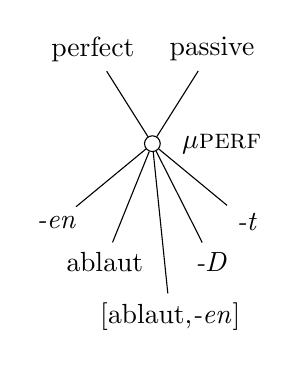
\begin{tikzpicture}[draw=black!100]
	\def \rowatticone{4.0cm}
 	\def \rowtwoht{3.5cm}
	\def \rowtwohta{3.2cm}
 	\def \rowoneht{2cm}
	\def \rowzerohta{0.8cm}
	\def \rowzeroht{0.5cm}
	\def \basementone{0.0cm}
 	\tikzstyle{ms-node}=[text centered]
 	\tikzstyle{m-node}=[circle,draw=black!100,thin,inner sep=0pt,minimum size=2mm]
	\tikzstyle{pf-node}=[text centered]
 	\tikzstyle{m-lbl}=[text width=5ex]
	\node[m-lbl] (label0) at (13ex,\rowoneht) {$\mu{\textit{\textsc{perf}}}$};
	
 	% morphosyntax
 	\node[ms-node] 	(ms0)	at (3ex,\rowtwohta)		{perfect};
 	\node[ms-node] 	(ms1)	at (13ex,\rowtwohta)	{passive};
	
 	% morphome
 	\node[m-node] 	(m0)	at (8ex,\rowoneht)		{};
	
	%phonological form
	 \node[pf-node] 	(pf0)	at (0ex,1cm)		{\textit{-en}};
 	\node[pf-node]  	(pf1)	at (4ex,\rowzeroht)		{ablaut};
 	\node[pf-node]  	(pf2)	at (9.5ex,-0.2cm)	 	{[ablaut,\textit{-en}]};
 	\node[pf-node]  	(pf3)	at (13ex,\rowzeroht) 		{\textit{-D}};
 	\node[pf-node] 	(pf4)	at (16ex,1cm) 		{\textit{-t}};	
	
 	\path (pf0)	edge	node	{}	(m0)
 		(pf1)	edge	node	{}	(m0)
 		(pf2)	edge	node	{}	(m0)
 		(pf3)	edge	node	{}	(m0)
		(pf4)	edge	node	{}	(m0)
		(m0) edge node 	{}	(ms0)
		(m0) edge node 	{}	(ms1);
		%(label0) edge node {}      (m0);	
 \end{tikzpicture}
\label{fig:ppgraph}
\caption{In the terminology of \citet{aronoff:1994}, the English perfect participle  is a \emph{polyvalent polymorphous} morphome; i.e., it has multiple functions (polyvalent) as well as multiple forms (polymorphous). The downward arcs represent form types, each of which is a \emph{meromorphomes.}}
\end{mdframed}
\end{figure}

\paragraph{Meromorphomes.} Whereas rhizomorphomes and metamorphomes 
are abstract, representing trans-lexemic and inter-paradigmatic relationships, %the realms of  lexemes and paradigms and thus highly 
meromorphomes are comparatively concrete. Meromorphomes 
correspond to particular parts of word forms. They 
are technically not the word parts themselves, as all morphomes reside at the 
morphomic level rather than the phonological, or surface, level \citep{round:2011}. 
Even so, meromorphomes map directly onto phonological forms, and 
are thus more closely associated with phonological forms than rhizomorphomes 
and metamorphomes. Indeed, both rhizomorphomes and metamorphomes are themselves
composed of meromorphomes, since, at some point, abstract, trans-lexemic 
morphomes must interact with specific phonological forms. 

For instance, in English perfect participles, each individual root, e.g., \textit{s-\textipa{2N}}, 
\textit{br.k}, \textit{\textipa{kIk}}, etc., is a meromorphome, as is each suffix (e.g., \textit{-ed}, \textit{-en}, etc.}
and each distinct variety of ablaut (e.g., \textit{br\textbf{ea}k/br\textbf{o}ken}, \textit{s\textbf{i}ng/s\textbf{u}ng}, etc.) is also a meromorphome. 
The Romance L-morphome is likewise composed of particular meromorphomes. 
Within the paradigm of the lexeme \textsc{decir} \textsc{`to say'} 
(see table~\ref{subtab:digo}), the stem \textit{dig-} is a meromorphome. 
Similarly, the stem \textit{crezc-} is a meromorphome within the paradigm of 
\textsc{crecir} \textsc{`to grow'} (see table~\ref{subtab:crezco}).

\begin{table}[ht]
\centering
\subtable[maqomi `local']{
\setlength{\extrarowheight}{8pt}
\begin{tabular}{lcc}
\toprule
& \textsc{masc} & \textsc{fem}  \\
\cmidrule{2-3} 
\textsc{sg} & maqom-i & meqom-i-t  \\
\textsc{pl} & meqom-iy-im & meqom-iy-ot  \\
\bottomrule
\end{tabular}
}
\subtable[gadol `big']{
\setlength{\extrarowheight}{8pt}
\begin{tabular}{lcc}
\toprule
& \textsc{masc} & \textsc{fem}  \\
\cmidrule{2-3}
\textsc{sg} & gadol & gdol-a  \\
\textsc{pl} & gdol-im & gdol-ot  \\
\bottomrule
\end{tabular}
}
\caption{Fusional suffixes in Hebrew nominals}
\label{tab:fusion}
\end{table}

\subsection{An example from Hebrew}
\label{sec:heb-example}
We turn now to a case of syncretism in the morphology of Modern Hebrew. Perhaps
the best known aspect of Hebrew (and Semitic languages in general) is its 
non-concatenative root-and-pattern morphology. But 
Hebrew's morphology also has a rich concatenative component, consisting of
of both inflectional and derivational affixes. 
Moreover, the inflectional affixes tend to be
highly %(and idiosyncratically) 
fusional. This illustrated in table~\ref{tab:fusion}: The suffixes for `masculine plural' and `feminine plural'
cannot be broken down into smaller gender and number components. 
%is 
%Consider, for example, the adjective inflections in table~\ref{tab:fusion}:

In this section, we will primarily be concerned with the
interaction between \textit{-t} and \textit{-i} in Hebrew feminine endings.
Hebrew uses the vowel [i] 
in both noun-deriving and adjective-deriving suffixes. 
As illustrated in table~\ref{subtab:der-adjectives}, 
one can derive adjectives 
in Hebrew by attaching \textit{-i} to noun bases. Thus,
 \begin{exe} 
\ex \label{ex:finished}
\begin{tabbing}
\hspace{.9in} \= \hspace{.4in} \= \hspace{.5in} \= \hspace{.4in} \= \hspace{.9in} \kill %\= \hspace{.3in} \= \hspace{1in} \kill
merxav \> $+$ \>  -i \> $=$ \>  merxavi \\
`space' \textsc{m.sg}   \> \> \textsc{adj} \>  \> `spatial' \textsc{m.sg}  \\
%\> \>  \>  \> \textsc{m.sg}
\end{tabbing}
%noun (\textsc{m.sg}) \> \> \> \> \> adj (\textsc{m.sg}) \\
%\textsf{matxilim} \> \textsf{\textbf{matxil+im}\$\$part\&root:txl\&ptn:hifil\&gen:ms\&num:pl}\, \\
%\> \textsf{\textbf{matxil+im}\$\$adj\&root:txl\&ptn:tbd\&gen:ms\&num:pl}
%\end{tabbing}
\end{exe}
The \textit{-i} 
must be the `adjective' exponent
in table \ref{subtab:der-adjectives} because it is the only suffixal 
element to occur in each
of the four columns. % It must therefore be the adjectival exponent in these cases. 

\begin{table}[ht]
   \centering
   \subtable[Adjectives derived from nouns via \textit{-i}\label{subtab:der-adjectives}]{
     \centering
     \setlength{\extrarowheight}{8pt}
        \begin{tabular}{l l l l c}
       \toprule
        \textsc{noun base} &  \textsc{masc.sg} & \textsc{fem.sg} &  \textsc{fem.pl} & \textsc{gloss} \\ %[0.5ex]
        \midrule
        %tarbut \textit{`culture'} & tarbut-i & tartbut-i-t & tarbut-iy-ot & `cultured' \\
        %le\textipa{P}om \textit{`nation'} & le\textipa{P}omi & le\textipa{P}omit & le\textipa{P}omiyot  & `national' \\
        merxav \textit{`space'} & merxav-i  &  merxav-i-t  &  merxav-iy-ot   &  `spatial' \\
        \textipa{P}aviv \textit{`spring'} & \textipa{P}aviv-i & \textipa{P}aviv-i-t & \textipa{P}aviv-iy-ot  & `spring-like' \\
        \textipa{P}arec \textit{`land'} & \textipa{P}arc-i & \textipa{P}arc-i-t & \textipa{P}arc-iy-ot  & `earthly' \\
        \bottomrule 
    \end{tabular}
   }\\
\vspace{6pt}
      \subtable[Nouns derived via \textit{-it}\label{subtab:der-nouns-i}]{
      \setlength{\extrarowheight}{8pt}
     \centering
     
    \begin{tabular}{l l l c} % creating 3 columns
   \toprule
    \textsc{base} &  \textsc{sg} &  \textsc{pl} & Gloss \\ 
    \midrule
    %pax \textit{`tin'} & pax-it & pax-iy-ot & `tin can' \\
    ma\d{s}a\textipa{P} `cargo' & ma\d{s}a\textipa{P}-it  &   ma\d{s}a\textipa{P}-iy-ot  &   `truck'   \\
    xalal \textit{`space'} & xalal-it & xalal-iy-ot & `spaceship' \\
    %k.r.k \textit{`(to) wrap'} &  kru\d{k}-it   &   kru\d{k}iy-ot  & `strudel' \\ %(iff \textit{fem}) or \\
    nagar \textit{`carpenter'}  &  nagar-it   &   nagr-iy-ot  & `female carpenter' \\
    \bottomrule
    \end{tabular}
   }\\
   \vspace{6pt}
   \subtable[Nouns derived via \textit{-ut}\label{subtab:der-nouns-u}]{
   \setlength{\extrarowheight}{8pt}
     \centering
        \begin{tabular}{l l l c}
        \toprule
        \textsc{base} &  \textsc{sg} &  \textsc{pl} & \textsc{gloss} \\ %[0.5ex]
        \midrule
        ma\v{s}ma\textrevglotstop \textit{`meaning'} & ma\v{s}ma\textrevglotstop-{u}t & ma\v{s}ma\textrevglotstop-{u}y-ot & `importance' \\
	\v{s}agrir \textit{`ambassador'} & \v{s}agrir-ut & \v{s}agriruy-ot & `embassy' \\
        %b.g.r \textit{`(to) mature'}  &  bagr-ut  &  bagr-uy-ot  &  `matriculation exam' \\
        nagar \textit{`carpenter'} &  nagar-ut   &   nagr-uy-ot  & `carpentry' \\
        \bottomrule
	\end{tabular}
   }
   	\caption{Derivational and inflectional syncretism in Hebrew feminine endings}
	\label{tab:deriv}
\end{table}

%Thus, 
%\begin{center}
%\begin{tabular}{ccccc}
%merxav & + & -i & =  & merxavi \\
%noun `space' &  & \textsc{adj} &   & `spatial' \\
%noun (\textsc{m.sg}) &  & &   & adj (\textsc{m.sg}) \\
%\end{tabular}
%\end{center}

%\exg. 
%   J\'anos h\'aza\\ 
%   John house.his\\ \hfill Hungarian (Finno-Ugric, \emph{reference}) 
%   \glt    `John's house' 
%\bigskip
%\noindent{And thus},


%\begin{equation*}
%\textit{merxav} \,\,\, \text{`space'} \quad + \quad \textit{-i} \quad  = \quad \textit{merxavi} \,\,\, \text{`spatial'} \quad \text{(masculine singular)'}
%\end{equation*}
The feminine singular is obtained by attaching \textit{-t} to the masculine singular
form. Feminine adjectives thus end in \textit{-it}. 
Hebrew also uses \textit{-it} to derive nouns, usually by attaching it 
to nouns, as in in table~\ref{subtab:der-nouns-i}. 
The vast majority of nouns derived in this way are feminine in 
grammar, semantics, or both. 

In Hebrew, feminine words frequently 
end in \textit{-t}. Indeed, the co-occurrence of \textit{-t} and the feminine gender is 
too frequent to be the product of random chance \citep{faust:2013}.
In fact, \textit{-t} serves as an exponent of both grammatical (or \emph{inflectional}) 
gender as well as semantic (or \emph{derivational}) gender. For example, /-t/ 
is an inflectional ending in \textit{merxavit} `spatial (feminine singular)' 
(cf. the corresponding masculine form \textit{merxavi}). 
It is part of the feminine nominal derivational suffix \textit{-it}, which is used to 
derive semantically feminine nouns, as in in \textit{nagar-it} 
`female carpenter' (cf. \textit{nagar}`(male) carpenter'.) 
Tables~\ref{subtab:der-adjectives} and \ref{subtab:der-nouns-i} 
show additional
examples of these two disparate functions of \textit{-i}.

\subsubsection{A morpheme-based approach}
The ending \textit{-t}, when used as (part of) a suffix on 
nominal forms, is always accompanied by a vowel. 
In fact, it appears with each of Modern Hebrew's five vowels.
In singular-form endings, it appears with every vowel except 
\textit{o}: \textit{-at}, \textit{-(e)t}, \textit{-ut}, and \textit{-it}. 
It appears with \textit{o} in the feminine plural suffix \textit{-ot} 
also ends with \textit{t}.\footnote{The consonant /t/ occurs with 
/o/ in singular forms as well, but only when /-ot/ is part of a 
primitive word, as in, e.g., \textipa{P}ot `letter'.}

Besides \textit{-t}, the only other systematic feminine marker is 
\textit{-a}, which is found only 
in feminine-singular absolute-state (i.e., \emph{free}) forms. %[Examples]
But a final \textit{-t} appears even in these nouns when they are 
in the construct state, a type of form which is used compound-noun 
construction and marked by its complete lack of stress.
\cite{schwarzwald:1982} argues that
the construct-state's \textit{t} ending was once also 
present on the absolute \textit{-a}, but was lost through a historical
\textit{t-}deletion process. \cite{faust:2013}, however, 
goes a step further, arguing that the \textit{t} remains 
underlyingly present in \textit{-a} even today. According 
to \cite{faust:2013}, both
\textit{-a} and \textit{-t} are underlyingly /-at/; sometimes 
the \textit{a} deletes, and sometimes the \textit{-t} deletes, depending 
upon certain phonological factors. Sometimes they appear 
together in the same form, as in feminine-singular construct nouns.
 Faust additionally decomposes the derivational endings 
\textit{-ut} and \textit{-it} into /u-at/ and /i-at/, respectively. 
The \textit{a} deletes in these forms.
Faust regards \textit{-et} in \textit{-at} as both allophones of /-at/. 
Faust's analysis of the Hebrew feminine endings thus constitutes a total of 
four morphemes, namely /-i/, /-u/, /-at/, and /-o/.
    
Faust's approach is based on Distributional Morphology 
 \citep{halle-and-marantz:1993}, 
a morpheme-based, Lexical-Realizational theory \citep{stump:2001}
According to Faust, therefore, the suffixes /-i/, /-u/, and /-at/ are not only morphemes, 
but \emph{roots.}
In Distributed Morphology (DM), the term \emph{root} (along with \emph{formative}) is used to refer 
to minimal (i.e., ``maximally primitive'') units of meaning. \footnote{However, is not to be confused with the 
consonantal root of Semitic morphology. Semitic roots would qualify as 
DM roots, but the DM root is more general than the Semitic root.}
A DM root has no particular morphosyntactic properties and thus belongs to 
no morphosyntactic category.
However, it does have abstract semantic features as well as inherent 
selectional requirements, that is, criteria that limit the set of stems with which it 
may combine. In particular, roots exclusively select 
other roots as their complements.  

Because \textit{-at} is a root, therefore, it
never attaches to derived stems. The same is true of /-i/ and /-u/.  
However, \textit{-at} is distinguished from /-i/ and /-u/ in that it occupies the 
position of category head in the derivation of adjectives.
In masculine adjectives, the category-head position is occupied by a phonologically null unit instead of
\textit{-at}, since \textit{-at} is a feminine suffix. %he \textit{-at} suffix is not present; % the suffix /-at/ is not itself present in the derivations of 
%masculine adjectives,
%It is just phonologically null, according to DM.
In masculine adjectives, therefore, the suffix /-i/ simply combines with the null adjectival head. 
This, according to Faust, satisfies the selectional requirements of /-i/
and the null adjectival head. The rest of the derivation,
proceeds as it does in feminine adjectives. 

According to Faust, \textit{-at} sometimes uses \textit{-i} and 
\textit{-u} as buffers. That is, it first attaches to \textit{-i} or \textit{-u}, 
thus forming complex units, either \emph{-it} or \emph{-ut}, respectively, 
which then attach to
the non-primitive stem. Because \emph{-it} and \emph{-ut} are complex, 
they cannot be roots and are thus free of roots' selectional constraints.

Moreover, Faust argues that the adjectival \textit{-i} and 
the noun-deriving \textit{-i} ending in tables 
\ref{subtab:der-adjectives} and \ref{subtab:der-nouns-i} 
are in fact one and the same expletive morpheme. That is, 
/-i/ does not \textit{per se} mean `\textsc{adjective}' in the derived adjectives 
\ref{subtab:der-adjectives}. Rather, it is an expletive suffix, one that 
crucially, for Faust, lacks morphosyntactic properties.
It is the theory of Distributed Morphology that motivates Faust's decision to posit a single 
expletive /-i/ morpheme (as opposed to 
separate adjective-deriving and noun-deriving morphemes).  Faust 
requires /-i/ to be a DM root so that /-at/ can combine with it, and since 
DM roots must be free of any specification of morphosyntactic 
category, an intrinsically adjectival /-i/ would
not suit Faust's DM analysis. 

\subsubsection{A \emph{morphome}-based approach}
Faust's account is similar to a \emph{morphome}-based account
in one respect, namely, in its analysis of /-i/
as a single (unified) morphological unit. But whereas Faust posits a unified 
/-i/ morpheme, we shall posit here a 
a unified \emph{morphome} $\mu{\textsc{i}}$. Like Faust's expletive /-i/,
$\mu{\textsc{i}}$ has no meaning in and of itself, but this is not 
because $\mu{\textsc{i}}$ is entirely unassociated with meaning; 
$\mu{\textsc{i}}$ lacks intrinsic meaning because meaning is not the 
purview of a morphomic representation. Rather, meaning is supplied by 
the lexical level. One of the advantages of a morphomic approach
is that any number of different meanings can be mapped onto a single 
morphome. We shall also posit a morphome corresponding to the 
feminine ending \textit{-a} and a \emph{different} morphome for 
\textit{-t}, as there does not seem to be enough synchronic evidence to posit that 
\textit{-a} and \text{-t} both have the \emph{synchronic} 
underlying form /-at/.
 \begin{figure}[t]
  \small
%\begin{center}
\centering
   \subfigure[{\textglotstop}{avavit} `spring-like'\label{subtab:heb-avivit}]{
     \centering
     \setlength{\extrarowheight}{8pt}
        \begin{tabular}{l c c c}
       \toprule
        \multicolumn{4}{c}{[\textipa{P}avivit] `spring-like'}\\
        \midrule
        \multirow{2}{*}{Phonological} & \textipa{P}aviv & -i & -t \\ %\hline
         & $\Phi${\textsc{stem}} & $\Phi${\textsc{i}} & $\Phi${\textsc{t}} \\
       Morphomic & $\mu$\textsc{a.i}, $\mu$\textsc{\textipa{P}.b.b} & $\mu{\textsc{i}}$  & $\mu{\textsc{t}}$ \\ 
        Lexical & \multicolumn{3}{c}{$\mu$\textsc{\textipa{P}.b.b}, \{\text{adj}, \text{fem}, \text{sg}\}}\\
        \bottomrule 
    \end{tabular}
    }
    \vspace{6pt}
      \subfigure[xalalit\label{subtab:heb-xalalit}]{
     \centering
     \setlength{\extrarowheight}{8pt}
    \begin{tabular}{l c c}
       \toprule
          \multicolumn{3}{c}{[xalalit] `spaceship'}\\
        \midrule
          \multirow{2}{*}{Phonological} & xalal & -it \\
           & $\Phi$\textsc{stem} & $\Phi$\textsc{it} \\
           Morphomic & $\mu$\textsc{a.a}, $\mu$\textsc{x.l.l} & $\mu$\textsc{i}, $\mu$\textsc{t} \\ 
            Lexical & \multicolumn{2}{c}{$\mu$\textsc{x.l.l}, \{\text{noun}, \text{fem}, \text{sg}\}}\\
       \bottomrule 
    \end{tabular}
    }
          \vspace{6pt}
  \subfigure[xalaliyot `spaceships'\label{subtab:heb-xalaliyot}]{
  \setlength{\extrarowheight}{8pt}
    \centering
        \begin{tabular}{l c c c }
       \toprule
        \multicolumn{4}{c}{[\textipa{x}alaliyot] `spaceships'}\\
        \midrule
        \multirow{2}{*}{Phonological} & xalal & -i & -ot \\ 
         & $\Phi$\textsc{stem}
         %s( \text{a.i}, \text{\textipa{P}.b.b} )$ 
         & $\Phi$\textsc{i} & $\Phi$\textsc{ot} \\ 
        Morphomic & $\mu${\textsc{a.a}}, $\mu$\textsc{x.l.l} & $\mu$\textsc{i}  &  $\mu$\textsc{o}, $\mu$\textsc{t} \\
                            %\multicolumn{2}{c}{$\mu$\textsc{o}, $\mu$\textsc{t}} \\ %\hline
        Lexical & \multicolumn{3}{c}{$\mu$\textsc{x.l.l}, \{\text{noun}, \text{fem}, \text{pl}\}}\\
        \bottomrule 
       \end{tabular}
  }
    \caption{Morphomic analyses} 
     \label{tab:heb-morphomic-analyses} 
    %\end{center}
    \end{figure}
 Finally, we posit distinct morphomes for the abstract (-\textsc{concrete}) 
 nominalizing suffix \textit{-u}
 as well as the \textit{-o} in the feminine plural \textit{-ot}.
That is, following \cite{faust:2013}, we shall
decompose not only /-it/, but /-ut/ and /-ot/ as well. 

  Accordingly, we need a total of five morphomes
  to account Hebrew's range of feminine suffixes. These are presented in table \ref{tab:heb-morphomes}. 
  Note that the mapping from 
  morphomes to phonological suffixes is not one-to-one. For example, 
  $\mu{\textsc{i}}$ maps to the adjective-deriving suffix /-i/. It also 
  plays a part in the realization of the noun-deriving suffix /-it/. Now, 
  this noun-deriving /-it/ is a single \emph{non-decomposable} suffix at the phonological 
  level. The evidence for this is the fact that the /t/ cannot be detached 
  from the /i/ when /-it/ is serving a noun-deriving purpose. Consider, for 
  example, nagar-it `female carpenter', which is derived from the suffix-less, 
  masculine noun base \emph{nagar} `(male) carpenter'. 
There is no *\emph{nagar-i}.
  
  
     \begin{table}[t]
\setlength{\extrarowheight}{8pt}
     \centering
       \begin{tabular}{ccc}
       \toprule
        \textsc{Morphome} &  \makecell{Phonological suffixe(s)} & Morphosyntactic property set(s) \\ %[0.5ex]
        \midrule
       $\mu{\textsc{a}}$ & {/-\textbf{a}/}, {/-\textbf{a}t/} & \makecell{\{fem, sg,\textsc{state:}abs\}, \\
       \{fem, sg, \textsc{state:}construct\}}\\
       $\mu{\textsc{i}}$ & {/-\textbf{i}/, /-\textbf{i}t/} & \text{n}$\to${adj}, \text{n}$\to$\text{n}[fem] \\
       $\mu{\textsc{u}}$ & {/-\textbf{u}t/} & \text{n}$\to$\text{n}[fem, -concrete] \\
       $\mu{\textsc{o}}$ & {/-\textbf{o}t/} & \{fem, pl\} \\
       $\mu{\textsc{t}}$ & \makecell{/-\textbf{t}/, /-o\textbf{t}/, /-u\textbf{t}/, /-i\textbf{t}/}  & \{fem\}, \{fem, pl\}, \{fem, -concrete\} \\
        \bottomrule 
    \end{tabular}
    \caption{Morphomic and phonological operations}
      \label{tab:heb-morphomes}
    \end{table}
    
Together, $\mu\textsc{i}$ and $\mu\textsc{t}$ form what is in effect  
a \emph{complex morphome} \citep{round:2015, round:md:2016}. A single 
phonological operation maps $\langle \mu\textsc{i}$, $\mu\textsc{t} \rangle$ 
onto a single morphological unit in the phonological output, namely the 
noun-deriving /-it/. The formation of the complex morphome $\langle \mu\textsc{i}$, 
$\mu\textsc{t} \rangle$ is conditioned upon presence of the 
property \{\text{n}$\to$\text{n}[fem] among the derivational properties $\delta$.

  By contrast, consider the masculine singular adjective form \emph{\textglotstop{aviv-i}} 
  `spring-like', derived from the \emph{\textglotstop{aviv} `spring'}, 
  as well its feminine-adjective inflection  \emph{\textglotstop{aviv-i-t}}. Here, the /-t/ 
  is very much detachable; its removal simply produces the masculine form. We
  thus regard the feminine adjective ending as decomposable even at the 
  phonological level, and thus there can be no complex morphome $\langle \mu\textsc{i}$, 
  $\mu\textsc{t} \rangle$ at the morphomic level. The same morphomes are present in the 
  morphomic representation of \emph{\textglotstop{aviv-i-t}}, but they are each 
  independently mapped to phonological representations.
  
  It is important that the same morphomes be present in the morphomic 
  representations of both noun-deriving and adjectival instances of /-it/, 
  even if the mappings from morphomes to the phonological level are different. We 
  want to acknowledge that the identities of form are not accidental, 
  and that there is sameness here at some level. The purpose of the 
  morphomic level is to account for
  this sort of sameness.
  
 We shall analyze /-ot/, the feminine plural suffix, and /-ut/, the abstract (or \textsc{concrete:}[-])
 noun-deriving suffix, in a similar way. Both are monolithic suffixes at the phonological
 level, and both have complex morphomic representations. Again, the primary reason for this
 is that neither /-ot/ nor /-ut/ seem to be decomposable, at least not in a straightforward
 way; that is, /-ot/ as a whole is the feminine plural suffix. If /-t/ is the fem. suffix, then
 /-o/ should be plural suffix. If this were the case, we would expect to see
 /-o/ in the masculine plural ending, but the masculine plural suffix is in fact /-im/. The suffix /-ot/
 corresponds to the morphome pair $\langle \mu\textsc{o}$, $\mu\textsc{t} \rangle$, 
 as shown in table \ref{subtab:heb-xalaliyot}, and /-ut/ to $\langle \mu\textsc{u}$, 
 $\mu\textsc{t} \rangle$. Analyzed in this way, /-ot/ and /-it/ share the morphome 
 $\mu$\textsc{t} with /-it/, thus accounting for the fact that all three suffixes end 
 in /-t/. The morphome $\mu\textsc{t}$ is thus used both derivationally and 
 inflectionally, a kind of dual appropriation that is not unknown among the world's languages. 
 Round, for instance, has frequently observed it in Kayardild: ``[M]ost of the exponents 
 employed by the inflectional system are also used derivationally'' \citep[][p. 13]{round:2015}.

\section{Implications for ULM and Multimorph}

Because ULM systems do not have access to
semantic or syntactic features, they cannot learn pairings of form and meaning, 
and hence, they cannot learn classical morphemes (see section~\ref{sec:what-exactly}). 
They can, however, learn recurrent units of \emph{pure} form. 
Consider again, 
for example, the feminine endings of Hebrew. A ULM system would likely be 
able to discover facts (\ref{ex:Xi}) and (\ref{ex:Yi}) and from them deduce (\ref{ex:i-and-t}): 
\begin{exe} \label{ex:observations1}
\ex \label{ex:Xi} There are many stems $X$ such that both $X$ and $X\text{\textbf{i}}$ are 
attested as words.
 \ex \label{ex:Yi} There are many stems \textit{Y} such that both \textit{Y} and \textit{Y}\textbf{t} 
 are attested as words.
\ex Therefore, \textit{-i} and \textit{-t} are both morphological units. \label{ex:i-and-t}
\end{exe}

The following, on the other hand, may prove to be more difficult:
\begin{exe} \label{ex:observations2}
\ex  \label{ex:YequalsXi} For some $X$ and $Y$, $Y=X\text{\textbf{i}}$. 
\ex  \label{ex:YneXi} On the other hand, sometimes $Y \ne X\text{\textbf{i}}$; that is, for some stems 
$X$, there is an $X\text{\textbf{it}}$, but no $X\text{\textbf{i}}$. 
\ex Therefore, there must be, \textbf{in addition to} \textit{-i} and \textit{-t}, 
a distinct suffix \textit{-it}.
\end{exe}
In our morphome-based analysis of Hebrew feminine endings, we said 
that while \text{-it} was a unified suffix at the phonological level, its morphomic 
representation consisted of two distinct morphomes, namely the pair 
$\langle$$\mu$\textsc{i}, $\mu$\textsc{t}$\rangle$. 
This accounted
 not only for the identities of exponence between tables~\ref{subtab:der-adjectives} 
and \ref{subtab:der-nouns-i}, but also for the \emph{difference}: There is an \emph{independent} \textit{-i} suffix 
 in table~\ref{subtab:der-adjectives}, but not in % \emph{vs.} the absence of an independent \textit{-i} ending in 
 table~\ref{subtab:der-nouns-i}.

%It would likely be difficult, however, for most ULM systems to capture such subtlety. 
%Most ULM systems would probably tend to decompose \textit{-it} 
%into \textit{-i} and \textit{-t} wherever it should occur, regardless of its type---i.e., whether it be of the
%``$\text{Y} = \text{Xi}$'' type (\ref{YequalsXi}) or the ``$\text{Y} \ne \text{Xi}$'' type (\ref{ex:YneXi}). At the same time, 
If a ULM system should encounter these different types of the \textit{-it} ending, one way it could analyze them would be to decompose the \textit{-it} into \textit{-i}  and \textit{-t} in every instance.
Arguably, such an approach would not be incorrect,
% to decompose \textit{-it} in every instance, not even from a morphomic perspective,
since there are precisely two morphomes at work in generating \textit{-t}, \textit{-i}, and \textit{-it}, 
 namely $\mu$\textsc{i} and $\mu$\textsc{t} (see the `Morphomic' row in table~\ref{subtab:der-adjectives}).
One's evaluation of a system thus depends on one's interpretation of the output as well as one's view of the system's 
task. Is the system  expected to discover phonological units (or operators), e.g., $\Phi$\textsc{i} $\Phi$\textsc{t}, and $\Phi$\textsc{it}, or 
morphomes, e.g., 
$\mu$\textsc{i} and $\mu$\textsc{t}.\footnote{Strictly speaking, the output would not contain morphomes themselves, but rather the \emph{projections} of morphomes onto 
the phonological plane, since morphomes themselves do not have phonological substance.}

One could argue that while they are composed of surface-level characters,
they are closer to morphomes in nature than phonological forms.
 Multimorph's MCMM has only one layer of hidden nodes,
and thus Multimorph cannot learn hierarchical structure; rather, it can only learn 
flat structure, and so, from a theoretical point of view, at least, it is ill-equipped to learn
that the \textit{-it} described in (\ref{ex:YneXi}) is simultaneously 
both a unified whole and a composite structure,
decomposable at the morphomic level into the distinct morphomes 
$\mu$\textsc{i} and $\mu$\textsc{t}.
It is, however, capable of handling such a case in other ways. 
Recall, from chapter~\ref{ch:MCMM} 
that an MCMM can map multiple causes (multiple morphological units)
 to a single surface-level node. Thus, if Multimorph's MCMM finds 
 \textit{-i}, \textit{-t}, \textit{-it} as three distinct
 morphological units (or clusters), it is capable of mapping all three 
 to a single surface-level node (representing a single feature). 
 But when it maps multiple clusters to individual surface-level nodes, 
 it does not do so in a hierarchical way; i.e., \textit{-i}, \textit{-t}, \textit{-it} would
 all be at the same level. %, so to speak.

At any rate, no ULM system is going to be able to learn the full range of morphomic
phenomena. No ULM system is going to be able to identify a metamorphome in its full
 extra-lexemic, trans-paradigmatic glory. Such a capability would require some means
of keeping track of what different lexemes do in different paradigm cells, which would be tantamount
to possessing morphosyntactic knowledge, since paradigm cells, whether taken alone or in groups,
are morphosyntactic property sets. As we have already noted, ULM systems do not
have access to morphosyntactic information.

%Why?  \emph{morphomes}?
	Technically, according to \cite{round:2011}, morphomic 
	representations do not have form. Morphomes
	themselves are apparently abstract units, i.e., abstract in that 
	a single morphome may encompass many lexemes at once, and thus
	have no particular form. Such morphomes are rhizomorphomes (e.g.,
	Latin third-declension nouns) and metamorphemes (e.g., the Romance L-morphome and the English
	${\mu}\textsc{perf}$ morphome).

	Metamorphomes simultaneously involve two kinds of identity. These are \emph{intra-}paradigm and {inter-}paradigm identity: 
	\begin{enumerate}
		\item \textbf{\emph{Intra-}paradigm Identity}: complete or partial identity of exponence between two or more cells of the same paradigm. 
		\item \textbf{\emph{Inter-}paradigm Identity}: Multiple paradigms (i.e., for multiple lexemes) exhibit the same \emph{pattern} of intra-pattern identity, though not the same stems, as the lexemes are different.
	\end{enumerate} 
Any case of intra-paradigm identity involves at least one shared 
meromorphome. For example, within the paradigm of the lexeme 
\textsc{decir} \textsc{`to say'}, 
the stem \textit{dig-} is a meromorphome. Similarly, the stem \textit{crezc-} 
is a meromorphome within the paradigm of 
\textsc{crecir} \textsc{`to grow'}. Crucially, however, 
\textit{dig-} and \textit{crezc-} are \emph{not} the same meromorphome. 
A metamorphome is a case of inter-paradigm identity, a situation 
in which the same subset of paradigm cells across different lexemes 
exhibit the sharing of a meromorphome, 
though the particular meromorphome being shared differs from lexeme to 
lexeme. 

Metamorphomes are beyond the capabilities of Multimorph. 
That is, while Multimorph is capable of discovering \textit{dig-} and \textit{crezc-} as units of form, 
it cannot learn that \textit{dig-} and \textit{crezc-} are the same 
in some way, i.e., that they are both lexeme-specific instantiations of the
same metamorphome.

A morphomic representation by definition does not have form.
As Round puts it,``The morphomic level 
therefore expresses \textsc{identities} of form, without 
expressing the forms themselves'' \citep[][pp.220-221]{round:2011} (emphasis in the original).
Thus, all morphome varieties are abstractions to some degree. 
Technically, according to Round, not even 
meromorphomes have forms, not in and 
of themselves, even though they constitute the 
morphome type that is most closely associated with specific, concrete pieces of form. 

Recall from chapter~\ref{ch:MCMM} that Multimorph's MCMM consists of
of a hidden layer, a reconstruction layer, and a layer of
weights connecting each hidden node to each reconstruction (or surface) node
Multimorph, however, relies heavily on form. The hidden 
layer provides a layer of abstraction, as this is where 
clustering takes place: Each hidden node represents 
a particular cluster, while the weights emanating from
each hidden node represent the average feature vector for that
cluster. This average feature vector is more or less the intersection
of the words in the cluster, i.e., something like (but not exactly) 
the longest the common subsequence once the average feature vector
is converted back to sequences of characters. The average vectors, also known as
cluster centroids, are approximations of meromorphomes, 
particularly the meromorphomes
that are closest to surface forms, i.e., not $\mu${\textsc{perf}}, 
for example, but rather $\mu${\textsc{en}},
$\mu${\textsc{d}}, etc.
%Multimorph 
%computes a centroid, i.e., an average feature vector. 
%This average feature vector  can be converted to a subsequence 
%that nearly every word in the cluster has in common. 
%This is basically what a meromorphome is.

One must rely heavily on form to find morphomes. One 
must infer facts about morphomic representations
from evidence observed in surface forms. Form is thus the 
gateway to the morphomic level. Without first observing 
some shared aspect of form, i.e., some identity of exponence, 
one cannot posit a morphome. Moreover, shared aspects of form 
can be observed only at the phonological level.
Identity of exponence is important not just to a morphomic analysis,
but also to Stump's Paradigm Function Morphology, especially where the 
the form paradigm is concerned, and indeed, it is central to any 
brand of autonomous morphology. It is thus appropriate that ULM 
systems---Multimorph included---are driven by form.

\section{Summary}\label{sum}
The notion of an autonomous morphological level
has been substantiated by a wealth research \citep[including, e.g.,][]{stump:2001, aronoff:1994, round:2011, round:2015}.
There is a rich and complex 
world between the planes of syntax and phonology, namely the world of autonomous morphology, which is free of both form and meaning. This is thus not the world of classical morphemes (pairings of form and meaning), but rather a new sort of morphological unit that mediates between phonology and
syntax/semantics, but is beholden to neither.  
Among the most notable formulations of autonomous morphology to date are Paradigm Function Morphology \citep{stump:2001}, particularly in the workings of its form-paradigm cells, Arornoff's
concept of the \emph{morphome} \citep{aronoff:1994}, and Round's expansions \citep[e.g.,][]{round:2011,round:2015} of Aronoff's original concept. The ever growing body of work on autonomous morphology vastly clarifies what ULM's target of learning is. Round's maxim in particular provides an implicit suggestion for how a ULM algorithm might proceed with its learning task: \textit{Look for similarities in form, since shared elements of form are indicators of shared morphomes.} Even though these morphomes, according to Round, have neither meaning nor form, they do, however, project something of themselves onto the phonological (or surface) level, since it is the surface level---particularly shared  form at the surface level, that allows us to identify morphomes in the first place. 

Therefore, in evaluating the present study's ULM system, namely Multimorph, one should not look for classical morphemes in its output, but rather autonomous morphological units like morphomes. (We will being use the term \emph{morphs} when referring to Multimorph's targets of learning.)
In the next chapter, our discussion turns to Multimorph itself and the setup of the experiments by which it was evaluated.
%we discuss the setup of the experiments by which Multimorph was evaluated. %
\chapter{Multimorph}
\label{ch:experi}
\section{Introduction}\label{sec:experi-intro}
%This chapter will describe the experimental setup,
This chapter will be concerned with the unsupervised morphological learning system Multimorph. Chapter~\ref{ch:MCMM} described the Multiple Cause Mixture Model (MCMM), a general unsupervised learning model (or algorithm). An MCMM serves as the core learning algorithm of Multimorph. The present chapter
% describes a particular morphological learning system that uses an MCMM as its core learning algorithm MCthe 
 describes the steps necessary to transform an MCMM into Multimorph,
% up into Mu   fully realized morphological learning system 
%chapter~\ref{ch:MCMM}. 
to bridge the gap between the general core and the fully realized system. 
% a particular unsupervised morphological learning system. 
For instance, one crucial matter discussed in this chapter is the question of \emph{features}, the elemental data descriptors that shape Multimorph's view of its input data and provide a common framework for establishing relations between data points. %(through its MCMM) relates one data point to another. 
Also in this chapter, we describe the preparation of Multimorph's input data an the key experimental variables that factored into Multimorph's evaluation.
%that is, the steps I took to prepare for and run the experiments. 

This chapter's discussion
is divided into two main sections: The first, section~\ref{sec:datasource}, concerns the extraction of the input data, including a description of the original data source. The second, section~\ref{sec:expvars}, discusses the experimental variables. The experimental variables comprise two broad categories: 
\begin{enumerate}
\item The representation of the input data. (For instance, the input words could be represented orthographically, according to the spelling conventions of Modern Hebrew, or they could be transcribed in some way.) The three choices for data representation are described in section~\ref{sec:datarep}.
%(i.e., orthographic vs. transcriptional) 
\item The precise definitions of the feature types, which varied according to the values of certain feature parameters. These parameters are discussed in section~\ref{sec:features}.
\end{enumerate}  

Multimorph can take as input \emph{any} list of words. The words can be of any
language, although Multimorph does expect the input strings to be composed
of alphabetic symbols. It also assumes that each symbol will be atomic rather
than composite. 
For example the symbol \textsf{\textipa{\.*k}} can be represented in Unicode either 
as a sequence of two code points, namely \texttt{U+006B, U+0323} 
(where \texttt{U+0323}
corresponds to the dot), or as the \emph{single} code point \texttt{U+1E33}. 
In its present form, Multimorph 
expects the latter. I mention this because the data source 
expresses
such characters in the former way, i.e., as sequences of code points. I thus had
to map the sequences onto atomic code points such as \texttt{U+0323} 
for \textsf{\textipa{\.*k}}.

When Multimorph reads the input wordlist, 
it maps each word onto
a sequence of 1s and 0s called a \emph{feature vector}, 
where each 1 or 0 is the value of a
particular feature. 
Features often follow some sort of template such as $\alpha$@[x], i.e., `character $\alpha$ occurs at position $x$' where $x$ is a member of an appropriate range of integers. This feature template can instantiated as many different specific features, and thus it constitutes a feature family (or category, type, etc.). The question of which feature types (as well as which particular feature instantiations) are most effective is one of this dissertation's research questions. 

\section{Data Source: The Berman Longitudinal Corpus}
\label{sec:datasource}
\subsection{Corpus Overview}
\label{sec:corpus-overview}
The input datasets (i.e., wordlists) were extracted 
from the BLC, \citep{berman-weissenborn:1991}. 
The BLC is part of the Hebrew section of the 
CHILDES Corpus \citep{macwhinney:2000a}, a corpus 
of transcribed conversations between young children 
and adults. I chose the BLC because 
it is one of the few sources of \emph{transcribed} Modern Hebrew. 
Most other Hebrew sources consist of printed material, 
such as newspaper text, and thus is orthographic 
rather than transcribed. The Hebrew alphabet has no 
dedicated letters for vowels, and thus Hebrew 
orthography is largely without vowels. I wanted data in which the vowels were 
fully represented. Another advantage of the BLC is that 
it is quite extensive. It contains 110,819 utterances, which, in turn, comprise 417,938 word tokens (13,828 word types) \citep{albert-et-al:2012}.
I am unaware of a larger source of 
transcribed Modern Hebrew. 

Each file in the BLC is the transcription of a 
particular session. The participants, who are identified 
in each file's header, can include, for example, the parents,
 other relatives, such as a grandmother, 
the researcher (or \emph{investigator}) conducting the 
session, and the child him or herself, 
who is called the \emph{target child}. All participants 
were native speakers of Modern Hebrew. The BLC comprises 
the transcriptions of many individual recording sessions. 
Each child's sessions were conducted over a period of 
12 to 19 months. Each child was between 16 and 21 months 
old when his/her recording sessions began, and between 
28 to 39 months old ($2\frac{1}{3}$ to $3\frac{1}{4}$ 
years old) when they ended.

\begin{figure}[t]
\begin{mdframed}
\begin{tabbing}
\hspace{0.6in} \= \hspace{0.6in} \=  \hspace{0.5in} \= \hspace{0.6in} \= \hspace{3.4in} \kill
\textsf{*MOT:} \> \textsf{ma} \> \textsf{\textipa{P}\a'{i}ma\textipa{P}} \> \textsf{\textipa{P}o\textipa{\.*s}\a'{a}} \>  \textsf{ba\# mi\textipa{\.*t}b\a'{a}x ?} \\
\> \textit{What [is]} \> \textit{Mom} \> \textit{doing} \> \textit{in.\textsc{def}+kitchen ?} \\[6pt]
\textsf{\%mor:} \> \textsf{que|ma=what n|\textipa{P}\a'{i}ma\textipa{P}\&gen:fm\&num:sg\&stat:free=mother} \\
 \> \textsf{part|\textipa{P}a\textipa{\.*s}\a'{a}\&root:\textipa{P}\textipa{\.*s}y\&ptn:qal\&gen:fm\&num:sg-\a'{a}=do} \\
   \> \textsf{prep|be~det|ha n|mi\textipa{\.*t}b\a'{a}x\&gen:ms\&num:sg\&stat:unsp=kitchen ?}\\[6pt]
\textsf{\%gra:} \>	\textsf{1|3|ANONAGR 2|3|AAGR 3|0|ROOT 4|3|MPRE 5|6|MDET 6|4|APREP 7|3|PUNCT}\\[6pt]
\textsf{CHI:} \> \textsf{rox\a'{e}cet} \> \textsf{kel\a'{i}m .}\\
		\> \textit{Washing} \> \textit{dishes .}  \\[6pt]
\textsf{\%mor:} \> \textsf{part|rax\a'{a}c\&root:rxc\&ptn:qal\&gen:fm\&num:sg-et=wash} \\
    \>  \textsf{n|kli}\&\textsf{gen:ms\&num:pl\&pl:masc:match\&stat:free-\a'{i}m=tool .} \\[6pt]
\textsf{\%gra:} \> \textsf{1|0|ROOT 2|1|ANONAGR 3|1|PUNCT}
\end{tabbing}
\caption{Excerpt from the Berman Longitudinal Corpus (BLC)}
\label{fig:excerpt}
\end{mdframed}
\end{figure}
Figure~\ref{fig:excerpt} shows an excerpt from the BLC. 
This excerpt contains two utterances, one spoken by the 
target child (CHI), and the other by the child's mother (MOT).
The first utterance in figure~\ref{fig:excerpt} is that of mother,
who says, ``What is Mom doing in the kitchen?'' The child
then replies \textsf{[rox\a'{e}cet kel\a'{i}m]}, `Washing dishes.'\footnote{The BLC's gloss `tools' is a generic translation of the Hebrew \textit{kel\'{i}m}. However, the context here suggests `dishes'
as a better translation.}
I have inserted these English words as glosses in italics as additional 
rows of text beneath the rows of transcribed words in figure~\ref{fig:excerpt}. 
Note these two extra rows do not appear. 
in the actual BLC.

The asterisk (*) preceding the labels CHI and \textsf{MOT} 
indicates that these tiers are \emph{main} tiers, i.e.,  
utterance tiers. Each utterance is accompanied by two 
additional tiers, 
namely, a morphological tier, labeled \textsf{\%mor}, 
and a syntactic (or grammatical) tier, labeled \textsf{\%gra}. 
The syntactic tier is not relevant to the present thesis,
so we shall not refer to it further. The morphological tier 
has a hierarchical structure. At the highest level, it consists of a 
series of space-delimited morphological analyses, 
There is exactly one analysis for each word in the main tier.  
Each \emph{individual} morphological analysis consists
of \textit{morphosyntactic properties}. These are delimited by the 
ampersand symbol (\textsf{\&}). Morphosyntactic properties are 
generally expressed as feature-value pairs of the 
form \textsf{\textit{feature}:\textit{value}}, e.g., 
\textsf{gen:fm} (`gender: feminine'). 

In the remainder of this section, we shall first discuss the 
BLC's unique transcription system, a system that 
honors Hebrew orthography as much as it does its spoken 
pronunciation. We shall then discuss some key aspects of 
the BLC's morphological annotation scheme. The 
transcription system is important for the present study 
because the features
depend on the alphabet in which the data is represented.
 The morphological annotation 
is significant because  the BLC's morphological annotations must 
serve as raw material for creation of  the intrinsic evaluation's 
gold-standard categories (see chapter~\ref{ch:eval}). 

\subsection{Transcription System}
\label{sec:transcription}

\begin{table}[t]
\centering
%\caption{Transcription System of the Berman Longitudinal Corpus}
%\label{tab:blc-alphabet}
\subtable[Consonants\label{subtab:trans-cons}]{
\setlength{\extrarowheight}{8pt}
\begin{tabular}{c c c c c c c c c c c c c}
\toprule                     
\begin{cjhebrew}'\end{cjhebrew} & \begin{cjhebrew}b\end{cjhebrew} & \begin{cjhebrew}g\end{cjhebrew} & \begin{cjhebrew}d\end{cjhebrew} 
& \begin{cjhebrew}h\end{cjhebrew} & \begin{cjhebrew}w\end{cjhebrew} & \begin{cjhebrew}z\end{cjhebrew}& \begin{cjhebrew}.h\end{cjhebrew}
& \begin{cjhebrew}.t\end{cjhebrew} & \begin{cjhebrew}y\end{cjhebrew} & \begin{cjhebrew}k|\end{cjhebrew} & \begin{cjhebrew}l\end{cjhebrew} 
&\begin{cjhebrew}m|\end{cjhebrew}\\ 
\textipa{P} & b/v & g & d 
& h & w & z & x 
& \textsubdot{t} & y & k/\textsubdot{k} & l & m \\[12pt]
           \begin{cjhebrew}n|\end{cjhebrew} & \begin{cjhebrew}s\end{cjhebrew} & \begin{cjhebrew}`\end{cjhebrew} 
           & \begin{cjhebrew}p|\end{cjhebrew} & \begin{cjhebrew}.s\end{cjhebrew} & \begin{cjhebrew}q\end{cjhebrew} & \begin{cjhebrew}r\end{cjhebrew} 
           & \begin{cjhebrew},s\end{cjhebrew}/\begin{cjhebrew}+s\end{cjhebrew}
           & \begin{cjhebrew}t\end{cjhebrew} & & \begin{cjhebrew}z\end{cjhebrew}$^\prime$ & \begin{cjhebrew}g\end{cjhebrew}$^\prime$ & \begin{cjhebrew}.s|\end{cjhebrew}$^\prime$ \\
	  n & s & \textipa{Q} 
	  & p/f & c & q & r & \v{s}/\textsubdot{s} 
	  & t & &  \v{z} & \textipa{J} & \c{c} \\
\bottomrule
\end{tabular}
}
\subtable[Vowels\label{subtab:trans-vowels}]{
\setlength{\extrarowheight}{8pt}
\begin{tabular}{c c c c c}
%\hline
\toprule
a & e & i & o & u \\
\'a & \'e & \'i & \'o & \'u \\
%\hline
\bottomrule
\end{tabular}
}
\caption{Transcription System of the Berman Longitudinal Corpus}
\label{tab:blc-alphabet}
\vspace{6pt}
\end{table}

The BLC's transcription system, summarized in table~\ref{tab:blc-alphabet}, %~\ref{subtab:trans-vowels} and \ref{subtab:trans-cons}, 
eludes simple one-word 
characterizations such as ``orthographic,''
``phonetic,'' or ``phonemic.'' It is in fact a hybrid system, drawing
both from phonetics and orthography \citep{albert-et-al:2013}. 
It is a transcription system in some ways and a transliteration 
system in others. It is a transcription system in that it has 
five dedicated vowel symbols, 
namely \{a, e, i, o, u\}, each of which matches one of the 
vowels in Modern Hebrew's five-vowel inventory. 
At the same time, however, 
it is a \emph{transliteration} system in that it is sensitive to 
orthographic distinctions that Modern Hebrew does not have.
The present consonantal alphabet of Hebrew originated in the 
language's classical period, with each 
consonantal grapheme corresponding to 
a distinct consonantal phoneme in Classical Hebrew \citep{rendsburg:1997}. The alphabet itself
has remained largely unchanged 
into the present day \citep{weinberg:1975, ravid:2005}; i.e. it has the same letters as it 
did in antiquity. The phonemic inventory 
of Hebrew, however, has changed. Thus, the correspondence 
between the graphemes of the Hebrew
alphabet and the phonemes of Modern Hebrew is far from perfect. 
The consonant inventory of Modern Hebrew
has undergone a number of neutralizations, leaving 
Modern Hebrew with a smaller inventory of consonant phonemes than
Classical Hebrew had. %Hebrew had in the Biblical period (i.e., the older part  
The mapping 
from consonantal graphemes in the Hebrew alphabet
to Modern Hebrew consonantal phonemes is therefore many-to-one.

\begin{table}[t]
\centering
\setlength{\extrarowheight}{8pt}
\begin{tabular}{l l c c c}
\toprule
 & Classical Hebrew  & Modern Hebrew   &  BLC  & Gloss \\
\midrule
a. & \textipa{kot\'eB}  & \textipa{kot\'ev} & \textipa{kot\'ev} & `writes, writing' \\
b. & \textipa{bor\'e\textbf{a}\textcrh} & \textipa{bor\'e\textbf{a}x} & \textipa{bor\'e\textbf{a}x} & `escapes, escaping'  \\
c. & \textipa{yod\'e\textbf{a}Q} & \textipa{yod\'e\textbf{a}} & \textipa{yod\'e\textbf{a}Q} & `knows, knowing' \\\bottomrule
\end{tabular}
\caption{\emph{a}-insertion before historical pharyngeals}
\label{tab:a-insertion}
%\vspace{3pt}
\end{table}

In its rendering of consonants, the BLC's transcriptional system 
favors orthography over actual pronunciation \citep{albert-et-al:2013}.
It honors a number of historical distinctions that have been preserved in the orthography, 
i.e., the alphabet and 
spelling conventions, but neutralized or otherwise lost in spoken Modern Hebrew. 
Table~\ref{tab:phon-neut} compares 
(reconstructed) Classical Hebrew phonemes, which are taken to be in a one-to-one 
correspondence with the letters of 
the Hebrew alphabet, Modern Hebrew speech sounds, and transcription symbols 
from the BLC. Notice that the
the Modern Hebrew column has the fewest distinctions.

\begin{table}[ht]
\centering 
\setlength{\extrarowheight}{8pt}
\begin{tabular}{l c c c}
\toprule
IPA & Orthography & BLC & Gloss  \\
\hline
    \textipa{[yad\'{a}]} &  \begin{cjhebrew}`dy\end{cjhebrew}  & \textipa{yad\'{a}Q} & `(he) knew' \\
    \textipa{[yad\'{a}]} &  \begin{cjhebrew}hdy\end{cjhebrew}  & \textipa{yad\'{a}h} &  `her hand' \\
\bottomrule
\end{tabular}
\caption{Ambiguity arising from the loss of consonantal distinctions.}
\label{tab:yada} 
\end{table}

The orthography of Modern Hebrew thus preserves the shadows of 
lost Classical Hebrew phonemes, as it were. 
Similarly, many morphophonological processes in Modern Hebrew
preserve residues of Classical Hebrew phonotactics and phonological processes. 
That is, even though the triggering contexts of these Classical Hebrew processes 
have been obscured or altogether lost due to sound changes, 
many have nonetheless been revived as fully-fledged components of Modern Hebrew. 
For example, in Classical Hebrew, the consonants \begin{cjhebrew}.h\end{cjhebrew} 
(\textit{\textipa{\textcrh{et}}}) and \begin{cjhebrew}`\end{cjhebrew}
(\textit{`ayin}) were both pharyngeal consonants; the former 
was a voiceless fricative (IPA \textipa{[\textcrh]}), and the latter a 
voiced stop (IPA \textipa{[Q]}). There was a process in Classical Hebrew 
whereby the [+low] vowel \textipa{[a]} was inserted between 
a [-low] vowel and a pharyngeal consonant to
mediate the transition between the [-low] vowel and the 
[+low] pharyngeal. This process is illustrated in table~\ref{tab:a-insertion}. 

Modern Hebrew, however, has no pharyngeals, having 
inherited its consonantal inventory 
largely from central and eastern European languages 
\citep{montoya:2014}. 
In Modern Hebrew, \textipa{[\textcrh]} 
is pronounced as a voiceless velar fricative 
(IPA \textipa{[x]}), and \textit{`ayin} 
is usually not pronounced at all. It has become 
phonologically 
equivalent to the historical glottal stop 
\begin{cjhebrew}'\end{cjhebrew} 
(\textit{'alef}). Both \begin{cjhebrew}'\end{cjhebrew} and 
\begin{cjhebrew}`\end{cjhebrew} 
are sometimes realized as glottal stops, but are 
often not pronounced at all, 
especially in fast speech \citep{matras-and-schiff:2005,berman:1985}. 
Nevertheless, Modern Hebrew has maintained the pre-pharyngeal 
\textit{a}-insertion process, as though the graphemes 
\begin{cjhebrew}`\end{cjhebrew} (\textit{`ayin}) and 
\textit{\textipa{\textcrh{et}}} still corresponded 
to phonological pharyngeals. This is shown in table~\ref{tab:a-insertion}:
In row (c), column Modern Hebrew, the \textit{a} is inserted 
even though the historical *\textipa{\textrevglotstop} 
(\textit{`ayin}) sound has vanished. In fact, no sound remains in this 
word-final position, not even a glottal stop for most 
speakers. The inserted \textit{a} thus ends up being the 
word's final phonological segment. And yet it is not the final segment
in the BLC's transcription, namely \textipa{yod\'eaQ} in row (c). 
The BLC includes the grapheme \begin{cjhebrew}`\end{cjhebrew} 
(\textit{`ayin}) in the form of the transcriptional 
symbol \textipa{[\textrevglotstop]}, as though it
were an actual speech sound.

Such a hybrid system offers both advantages and disadvantages to a 
ULM system like Multimorph. 
On the one hand, the inclusion of such lost consonants as 
\begin{cjhebrew}`\end{cjhebrew} 
(\textit{`ayin}) provides a system with additional and potentially 
quite valuable information. 
Phonemic mergers can obscure category memberships and thus 
create ambiguity. For instance, 
the forms for `(he) knew' and `her hand' in  table~\ref{tab:yada}
have identical pronunciations in Modern Hebrew, as indicated 
by their identical transcriptions in the International Phonetic Alphabet (IPA)
in \ref{tab:yada}. And yet they are different. 
The former is a 3rd-masculine-singular past-tense verb of the 
\emph{qal} binyan. Its root consists of the \emph{three}
consonants \textit{\textipa{y.d.Q}}, which one must 
know in order 
to connect this verb to derivationally related words. 
The second \textipa{[yad\`{a}]} 
in table~\ref{tab:yada} is the noun \textit{yad} plus 
the 3fs possessive suffix 
\textit{-a(h)}, the final \emph{h} of which is not articulated. 
Because the BLC's transcriptional system preserves 
certain consonants and 
inter-consonant distinctions, it preserves information and 
thus reduces ambiguity. 
This is probably going to be advantageous to a ULM 
system, even if the preserved 
information is not entirely accurate vis-\`{a}-vis Modern Hebrew 
pronunciation.

On the other hand, the inclusion of these non-Modern 
sounds means that more features are necessary to describe 
words. The larger number of features results in longer processing times. 
A larger number of features can also decrease accuracy 
if the additional features are not useful. 
In addition, increasing the number of symbols does not 
always help to clarify true relationships; sometimes it 
obscures them. For example, the BLC's transcriptions 
represent the spirantization of the certain oral obstruents; 
in particular, \textipa{/b/} $\to$ v, \textipa{/p/} $\to$ f, and \textipa{/k/} $\to$ \textsubdot{k} 
in the context
Vowel \_\_. Hence, the underlying \textipa{/b/} in the root \textit{k.t.b} 
(`\textsc{write}') often manifests as [v], as it does in \textit{katavti}
(`I wrote') and 
\textipa{\textit{yi{\.*k}t\'ov}} (`he will write'). The latter exhibits not only
the alternation 
\textipa{/b/}~$\to$~v, but also \textipa{/k/}~$\to$~\textsubdot{k}.
%two altered characters. 
Recall, however, from section~\ref{sec:experi-intro}, that even \textit{\textipa{\.*k}} looks like \textit{k} with a dot below it,
Multimorph would have seen them as entirely distinct symbols, just as \textit{\textipa{b}} and \textit{v} are distinct symbols.
In Multimorph's input data, \textit{\textipa{\.*k}} and \textit{\textsubdot{k}} were each represented as a  distinct atomic unicode character.
%Multimorph thus did not not see \textit{\textipa{\.*k}} and \textit{\textsubdot{k}} as fundamentally related. 
All unicode characters were atomic and monolithic. Symbols with dots (e.g., \textsubdot{k}) or accent marks (e.g., \'{u}) were represented as \textit{precomposed} unicode characters and thus were in effect as atomic as any other character.
%and \textit{k} as 
%entirely different symbols, not as allophones
%of the same phoneme. The same would be true for \textit{b} 
%and \textit{v}.  

%\begin{cjhebrew}yd`\end{cjhebrew}
%For the purposes of learning Hebrew morphology, this is probably useful information. 
%The more information the better, Dawg.
%For example, the presence of the phantom \textipa{Q} 
%probably makes it easier to identify the root 
%$\surd$y-d-\textipa{Q}

The grapheme \begin{cjhebrew}`\end{cjhebrew} (\textit{`ayin}) is not the only 
grapheme to have 
lost its ancient phonemic affiliation. 
The graphemes \begin{cjhebrew}.t\end{cjhebrew} 
(\textit{\textipa{\.*te\.*t}}), \begin{cjhebrew}s\end{cjhebrew} 
(\textit{\textipa{same\.*k}}), correspond to emphatic, i.e., 
pharyngealized, consonants in Classical 
Hebrew, probably pharyngealized versions of [s] of [t] \citep{matras-and-schiff:2005}.
Modern Hebrew, however, lacks pharyngealized consonants just as 
it lacks pharyngeals. 
The consonant \begin{cjhebrew}q\end{cjhebrew} (\textit{qof}, 
IPA \textipa{[q]}) was uvular and 
possibly pharyngealized in Classical Hebrew, but in Modern Hebrew, 
it has merged with the velar voiceless stop
\begin{cjhebrew}k|\end{cjhebrew} (\textit{kaf}, IPA \textipa{[k]}).
%Thus, 
%as the \emph{emphatic consonants}, were once associated with pharyngealized phonemes, but now they are pronounced simply as [s] and [t]. 
Similarly, the pronunciations 
%(or affiliated phonemes) 
of  \textit{\textipa{same\.*k}} and \textit{\textipa{\.*te\.*t}} 
have merged with those of \textit{sin} and \textit{tav} respectively, 
 so that \textit{\textipa{same\.*k}} and \textit{\textipa{sin}} 
 are both pronounced as [s], and \textit{\textipa{\.*te\.*t}} and 
 \textit{tav} as [t]. But whereas the phonemic inventory of 
 Modern Hebrew has lost distinctions, the Hebrew writing system has preserved several inter-consonantal distinctions.

\begin{table}[t]
\centering 
\setlength{\extrarowheight}{9pt}
\begin{tabular}{l c c c c }
\toprule
\multirow{2}{*}{Heb. Letter} & Special &  \multicolumn{2}{c}{IPA} & \multirow{2}{*}{BLC}\\\cline{3-4}
    & Context & BH  & Modern Hebrew & \\
\midrule
\begin{cjhebrew}'\end{cjhebrew} ('alef) & &  \textipa{P} & -- & \textit{\textsf{\textipa{P}}} \\
\begin{cjhebrew}`\end{cjhebrew} (`ayin) & &\textipa{Q} & -- & \textit{\textsf{\textipa{Q}}} \\
\begin{cjhebrew}q\end{cjhebrew} (qof )& & \textipa{q} & \textsf{\textipa{k}} & 
\textit{\textsf{\textipa{q}}} \\
\multirow{2}{*}{\begin{cjhebrew}k|\end{cjhebrew} (kaf)} & & \textipa{k} & \textsf{\textipa{k}} & \textit{\textsf{\textipa{k}}} \\
		         & {Vowel\,\_} & \textipa{x} &\textsf{\textipa{x}} & \textit{\textsf{\textipa{\.*k}}} \\
 \begin{cjhebrew}x\end{cjhebrew} (\textipa{\textsubdot{h}et}) & &\textipa{\textcrh} & \textsf{\textipa{x}} & \textit{\textsf{\textipa{x}}} \\
 \begin{cjhebrew}s\end{cjhebrew} (\textipa{same\.*k}) & & \textipa{\textsuperimposetilde{s}} & \textsf{\textipa{s}} & \textit{\textsf{\textipa{s}}} \\
  \begin{cjhebrew},s\end{cjhebrew} (\textipa{sin}) & & \textipa{\textbeltl}  &  \textsf{\textipa{s}} & \textit{\textsf{\textipa{\.*s}}} \\
 \begin{cjhebrew}.t\end{cjhebrew} (\textipa{\.*te\.*t}) & & \textipa{\textsuperimposetilde{t}}&  \textsf{\textipa{t}} & \textit{\textsf{\textipa{\.*t}}} \\
  \multirow{2}{*}{\begin{cjhebrew}t\end{cjhebrew} (\textipa{tav})} &  & \textipa{t} &  \textsf{\textipa{t}} & \textit{\textsf{\textipa{t}}} \\
& Vowel\,\_ & \textipa{T} &  \textsf{\textipa{t}} & \textit{\textsf{\textipa{t}}} \\
% \multirow{2}{*}{\begin{cjhebrew}b\end{cjhebrew} (bet)} & \multirow{2}{*}{Vowel\_} & \textipa{b} & \textsf{\textipa{b}} & \textit{\textsf{\textipa{b}}} \\
% &      	  & \textipa{B} & \textsf{\textipa{v}} & \textit{\textsf{\textipa{v}}} \\
 \multirow{2}{*}{\begin{cjhebrew}b\end{cjhebrew} (bet)} & & \textipa{b} & \textsf{\textipa{b}} & \textit{\textsf{\textipa{b}}} \\
		         & {Vowel\,\_} & \textipa{B} &\textsf{\textipa{v}} & \textit{\textsf{\textipa{v}}} \\
 \begin{cjhebrew}w\end{cjhebrew} (\textipa{waw}) & & \textipa{w} & \textsf{\textipa{v}} & \textit{\textsf{\textipa{w}}} \\
\bottomrule
\end{tabular}
\caption{Correspondences between Hebrew orthography, speech sounds (past and present), and the BLC's transcriptional system}
\label{tab:phon-neut}
\end{table}

\subsection{Morphological Annotation}
\label{sec:morph-annotation}
For our purposes, the most salient aspects the BLC's morphological 
annotation are those relevant to the tasks of
\begin{itemize}
\item extracting unified word tokens, each completely free of internal morphological 
delimiters or any other annotative device
\item extracting each word's corresponding morphological analysis from the 
\textsf{\%mor} tier, maintaining the one-to-one
correspondence between words and morphological analyses. 
\end{itemize} %are those that \citep{albert-et-al:2012}.
The morphological analyses themselves are essentially lists of morphological categories, 
i.e., lists of simple feature-value pairs.
The following is a BLC morphological analysis after undergoing the transformations 
described in section~\ref{sec:extr}:
\begin{exe} 
\ex \label{ex:finished}
\begin{tabbing}
\hspace{0.8in} \= \hspace{5.5in} \kill
\textsf{matxilim} \> \textsf{\textbf{matxil+im}\$\$part\&root:txl\&ptn:hifil\&gen:ms\&num:pl}\, \\
\> \textsf{\textbf{matxil+im}\$\$adj\&root:txl\&ptn:tbd\&gen:ms\&num:pl}
\end{tabbing}
\end{exe}
This example contains two separate analyses, a result of ambiguity. 
Each analysis is preceded by a segmentation (in boldface). 
In cases of ambiguity, i.e., of multiple analyses, each analysis gets its own 
segmentation, even though the segmentations may be identical.

\paragraph{Prefixal clitics.} In Hebrew, many functional words are 
\textit{prefixal clitics}; that is, they attach to content 
words as prefixes. They include the definite article \textit{ha-}, the prepositions 
\textit{le-} (`to, for') \textit{be-} (`in'), \textit{ke-} (`like/as'), and \textit{me-} 
(`from'), the  complementizer/relativizer \textit{\v{s}e-} (`that/which'), and the 
conjunction \textit{we-} `and.' For example,  in
\textsf{wehay\'eled} (`and the boy'), the prefixes \textit{we-} and \textit{ha-} 
are attached as clitics to \textit{y\'eled}, 
so that the whole is regarded as a single word. The 
BLC tokenizes these clitics, separating them from the 
main (content) word, and adding the number symbol (`\texttt{\#}') to 
the end of each prefixal clitic:
\begin{exe}
\ex  \textsf{wehay\'eled}  \quad $\mapsto$ \quad \textsf{we\# ha\# y\'eled}.
\end{exe}
%would be transcribed as \textsf{we\# ha\# y\'eled}.
The following example from the BLC, example~(\ref{ex:pphash2}), shows the morphological analyses accompanying the prefixal clitics \textit{we-} (`and') and \textit{\v{s}e-} (`that') as well as the morphological analysis of the main word.
% \textit{we-} (`and') followed by the complementer/relativizer \textit{\v{s}e-} (`that'), which is another prefixal clitic.  It also shows the corresponding morphological analyses.
\begin{exe}
	\ex 
	\textsf{we\#\, \v{s}e\# me\textipa{Q}arbev\'im} \\  \label{ex:pphash2}
	\textsf{conj|we conj:subor|\v{s}e\, part|\textipa{P}irb\'ev\&root:\textipa{Q}rbb\&ptn:piel\&gen:ms\&num:pl} 
\end{exe}

\paragraph{Demarcation of inflectional affixes.}
Past tense verbs take inflectional suffixes. Future-tense verbs take both inflectional prefixes and suffixes. 
Nominals, where inflection
is concerned, take only suffixes. The `\#' and `-' symbols are used to separate inflectional
affixes from the stem's morphological analysis; the `\#' used in the case of prefixes, `-' in the
case of suffixes, as in the following:

\begin{exe}
\ex \begin{tabbing} \label{ex:pre:v:suf}
\hspace{0.6in} \= \hspace{5.5in} \kill
\textsf{*CHI:} \> \textsf{tirt\a'{u} .} \\
\textsf{\%mor:} \> \textbf{\textsf{ti}\#}\textsf{v|ra\textipa{P}\a'{a}\&root:r\textipa{P}y\&ptn:qal\&tense:fut\&pers:2\&
\textbf{gen:unsp\&num:pl-\a'{u}}=see}
\end{tabbing}
\end{exe}

\paragraph{Compound and bound nouns}
Construct-state nouns are labeled either as ``\textsf{stat:bound}'' 
or ``\textsf{stat:comp}'' (i.e.,`compound'). 
These two labels correspond to the same sort of phonological form, 
 so I collapsed them into a single label, namely 
``\textsf{stat:cstr}'' (for `construct state').

\subsection{Anomalous Forms}\label{sec:anomolous}

Even though the BLC contains a good deal of adult speech, it also, 
of course, contains child speech, which  
can be rife with anomalies (anomalies relative to adult speech, that is). 
And while such anomalies are interesting if one is studying language acquisition 
in children, they are not helpful where the present study is concerned. It 
was therefore necessary to ``correct'' such anomalous forms where it was 
possible to do so, and discard them where it was not. Toward this end, 
the BLC's annotation conventions proved to be a great help.

\paragraph{Forms to be replaced}
The BLC deals with anomalous forms through a special 
annotative device consisting of a set of square brackets, with the left bracket 
accompanied
by a colon, i.e., 
\begin{center}
\textsf{[: \textit{corrected-form} ]}
\end{center}
Sometimes these brackets 
are followed by a second set of brackets, as in the following:
\begin{exe} \label{ex:tau}
\ex \textsf{tikri \,\textbf{[: tiqre\textipa{P}\a'{i}]}\, \textbf{[*]}\, sip\a'{u}r\, d\a'{o}da\, Orly .}
\end{exe}
This second set, if present, most frequently contains just an asterisk shown, as in example~(\ref{ex:tau}). However,
the asterisk may be followed
by an error classification. The first bracket pair (the one with colon) offers a correction for the preceding erroneous/anomalous form.

%However, since neither error categories nor errors were relevant to the present study, I discarded second bracket pair wherever it occurred, and I replaced anomalous/erroneous forms with their respective corrections.

% with the content in the first set of brackets ( %and was thus discarded. %discardethis second set of brackets was not
%(`*$\tau$') where $tau$ may be empty, or it may specify some error category. 
%In the BLC, it is most frequently empty. %, as in (\ref{ex:repl2}). 

%According to the CHILDES manual \citep{macwhinney:2000b}, the purpose 
%of the ``\textsf{[*$\tau$]}'' 
%is to specify that an anomalous form is 
%indeed erroneous rather than merely non-standard. 
%However, this distinction between 
%\textsf{[: \textit{corrected-form} ]} and 
%\textsf{[: \textit{corrected-form} ] [*{$\tau$}]} is not always manifest in BLC.
%In (\ref{ex:repl1}), the anomalous 
%form \textsf{patux} 
%(the `\textsf{@c} ' indicates a child-created form); 
%the anomaly is an absent \textsf{a} before the \textsf{x}, thus violating 
%a morphophonemic process 
%whereby \textit{a} is inserted before pharyngeals.\footnote{This is a process grandfathered in from
%from Classical Hebrew; its triggering context actually no longer exists, as Modern Hebrew no longer has pharyngeals (see section~\ref{tab:a-insertion}).}
%In (\ref{ex:repl2}), the error is essentially that the pre-\textit{\textipa{P}} 
%\textit{a} is absent. The glottal stop
%associated with the grapheme \begin{cjhebrew}'\end{cjhebrew} (\textit{'alef}) 
%is typically not articulated in Modern Hebrew \citep{montoya:2014}. The distinction
%between the two is not entirely clear.
%
%The distinction between , if there is one, is not important for our purposes. 
%Either way, I needed to replace the anomalous form with the form enclosed in 
%(the first pair of) brackets (see example~(\ref{ex:brackets})). We can just discard the \textsf{[*$\tau$]} 
%if it is present, regardless of what $\tau$ is.
%The important material for our purposes was between the first pair of brackets, as these brackets offer a correction of the preceding erroneous form. I replaced all erroneous forms with their respective corrections.
%\begin{exe}
%\label{ex:brackets}
%%\ex %\begin{xlist} 
%\ex\label{ex:repl1} 
%   %\ex\label{ex:repl1} 
%   \begin{tabbing}  
%  \hspace{0.6in} \= \hspace{5.5in} \kill
%  \textsf{*CHI:} \> \textsf{po ye\v{s} patux@c \textbf{[: pat\a'{u}ax]} d\a'{e}let .}
%  \end{tabbing}
%\end{exe}  
%     \ex\label{ex:repl2} \begin{tabbing}
%  \hspace{0.6in} \= \hspace{5.5in} \kill
%  \textsf{*CHI:} \> \textsf{tikri \,\textbf{[: tiqre\textipa{P}\a'{i}]}\, \textbf{[*]}\, 
%  sip\a'{u}r\, d\a'{o}da\, Orly .} \\
%  \textsf{\%mor:} \> \textsf{ti\#v|qar\a'{a}\textipa{P}\&root:qr\textipa{P}\&ptn:qal\&tense:fut\&pers:2\&gen:fm\&num:sg-\a'{i}=read} \\
%                    \> \textsf{n|sip\a'{u}r\&gen:ms\&num:sg\&stat:unsp } \\
%                    \> \textsf{n|dod\&gen:fm\&num:sg\&stat:free-a=uncle/aunt} \textsf{n:prop|Orly .}
%  \end{tabbing}
%   \end{xlist}
%\end{exe}


\paragraph{Dropped sounds}
The adults recorded in the BLC produced anomalous or non-standard speech, too. In example~(\ref{ex:dropped}), for instance, the investigator 
has dropped the 
\emph{n} from the infinitive form 
\textsf{li\textbf{(n)}s\'oa\textipa{Q}} (`to ride, drive, travel'), 
which is of the root \textit{n.s.\textipa{Q}}. 
The BLC's transcribers ``restored'' such dropped or deleted sounds and enclosed them in parentheses.
\begin{exe} 
\ex \label{ex:dropped} \textsf{li(n)s\a'{o}a\textipa{Q} \, ba\#\, \v{s}en\a'{i} ?}
\end{exe}

%\ex \begin{tabbing}
%\hspace{0.6in} \= \hspace{5.5in} \kill
%\textsf{*INV:} \> \textsf{li(n)s\a'{o}a\textipa{Q} \, ba\#\, \v{s}en\a'{i} ?}
%\end{tabbing}
%\end{exe}

\paragraph{Duplications}
Sometimes the BLC records speakers as having repeated a word or clitic, as in example~(\ref{ex:redundant}),
% (\ref{ex:redundant}), a prefixal clitic, 
%is duplicated, and sometimes repeated
%several times consecutively. 
The BLC records word repetiton (i.e., as part of dysfluency) even when it results in ungrammaticality.
%(as in a dysfluency), 
For example, (\ref{ex:redundant}) shows an utterance in which the prefixal clitic \textit{we\#} is 
attached to itself several times. No special annotation is used to mark or correct such repetitions. 
%Notice that morphological analysis for
%for \textit{we\#} is also repeated, so that each \textit{we\#} in the main tier has its ``own'' copy of the morphological analysis.
\begin{exe} 
\ex \label{ex:redundant} \textsf{*CHI:\quad we\# we\# we\# we\#\, nigm\textipa{\'a}r } \\
   \textsf{\%mor:\quad conj|we=and\, conj|we=and\, conj|we=and\, conj|we=and} \\
   \textsf{v|nigm\'ar\&root:gmr\&ptn:nifal\&tense:past\&pers:3\&gen:ms\&num:sg=be\_finished }
\end{exe}

%Observations: Note the number (or pound) sign \textsf{\#} at the end of the token \textsf{ba\#}. `in the', which is analyzed in the MA tier as $\texttt{prep|be}$$\sim$$\texttt{det|ha}$. 
%We handle this in different ways in the transcriptions vs. the morphoplogical analyses. Within the 
%morphological analysis tier, the analyses are delimited by spaces, with each single analysis corresponding
%to a word in the transcriptional tier. 
 
\section{Extracting the Input Datasets}
\label{sec:extr}
%To conduct the experiments, three input wordlists were necessary, 
The experiments required three input wordlists, one for each data-representation type. 
namely, a transcriptional list with stress markings (TS), a transcriptional list without stress markings  (TR), and an orthographic list (O).
The words in TS were composed of the BLC's transcriptional symbols, 
whereas those in O
were composed of regular Hebrew letters, following Hebrew spelling conventions. 
In O, the standard Hebrew letters were converted to ASCII characters in a one-to-one
mapping, namely the transliteration mapping of the Hebrew Treebank 
\citep{simaan-et-al:2001}, displayed in table~\ref{tab:ortho-alph}). %adgdhwzxviklmnsypcqret
\begin{table}[ht]
\setlength{\extrarowheight}{8pt}
\centering
\caption{Romanization of the Hebrew Alphabet \citep{simaan-et-al:2001}}
\label{tab:ortho-alph}
\begin{tabular}{c c c c c c c c c c c}
\toprule %\hline                      
\begin{cjhebrew}'\end{cjhebrew} & \begin{cjhebrew}b\end{cjhebrew} & \begin{cjhebrew}g\end{cjhebrew} & \begin{cjhebrew}d\end{cjhebrew} 
& \begin{cjhebrew}h\end{cjhebrew} & \begin{cjhebrew}w\end{cjhebrew} & \begin{cjhebrew}z\end{cjhebrew}& \begin{cjhebrew}.h\end{cjhebrew}
& \begin{cjhebrew}.t\end{cjhebrew} & \begin{cjhebrew}y\end{cjhebrew} & \begin{cjhebrew}k|\end{cjhebrew} \\ 
a & b & g & d 
& h & w & z & x & v & i & k \\[12pt]
\midrule
%& \textsubdot{t} & y & k/\textsubdot{k} & l & m \\[12pt]
 \begin{cjhebrew}l\end{cjhebrew} & \begin{cjhebrew}m\end{cjhebrew} &
           \begin{cjhebrew}n|\end{cjhebrew} & \begin{cjhebrew}s\end{cjhebrew} & \begin{cjhebrew}`\end{cjhebrew} 
           & \begin{cjhebrew}p|\end{cjhebrew} & \begin{cjhebrew}.s\end{cjhebrew} & \begin{cjhebrew}q\end{cjhebrew} & \begin{cjhebrew}r\end{cjhebrew} & \begin{cjhebrew},s\end{cjhebrew}/\begin{cjhebrew}+s\end{cjhebrew} & \begin{cjhebrew}t\end{cjhebrew} \\
          l & m &
	n & s & y & p & c & q & r & e & t \\
\bottomrule
\end{tabular}
\end{table}
O was obtained by mapping each transcriptional representation 
in TS onto an orthographic representation. For example, \textipa{hitkawanti}$_{TS}$ $\to$
\textipa{htkwnti}$_{O}$ and \textipa{katavti}$_{TS}$ $\to$ \textipa{ktbti}$_{O}$. 
The TR words were obtained by 
replacing the accented vowel characters in the TS list with their unaccented counterparts.
Also necessary were three sets of morphological segmentations, one for each dataset: %namely $\text{T}_{SEG}$ and $\text{O}_{SEG}$, where:
\begin{itemize}
\item $\text{TS}_{SEG}$ = segmentations for 10 percent of the words in TS.
\item $\text{TR}_{SEG}$ = $\text{TS}_{SEG}$, except with the accented vowels replaced
with unaccented vowels.
\item  $\text{O}_{SEG}$ = segmentations for 10 percent of the words in O.
\end{itemize} 
%A third set of segmentations TR
%Each acted as a gold-standard in the extrinsic 
%component of the evaluation phase. (see chapter \ref{ch:eval}).  

\paragraph{Replacement of Anomalous Forms.} 
The input datasets were extracted from the BLC. However, as noted above in 
section~\ref{sec:anomolous}, the BLC is by no means free of anomalous forms, 
forms that are ungrammatical with respect to the standard form of the language, 
forms that, for our purposes, would convey misinformation about the language if taken at face value. 
Such misrepresentative and potentially misleading forms were excluded from the 
extracted input data.  
Wherever a pair of brackets, i.e., \textsf{[: \textit{corrected-text} ]}, was encountered, 
the material within the brackets was extracted in place of the anomalous word (i.e., the 
word the preceding the ``\textsf{[:}'').

\begin{exe}
	\ex Replacing anomalous forms with their bracket-enclosed corrections
	\begin{xlist} \label{ex:replace}
	   \ex \textsf{*CHI:}\quad\textsf{po\, ye\v{s}\, \textbf{patux@c\, [: pat\'{u}ax ]}\, d\'{e}let} $\quad\to\quad$
	   \textsf{po ye\v{s} \textbf{pat\'{u}ax} d\'{e}let} 
	   \ex \textsf{*CHI:}\quad\textsf{\textglotstop\'{o}\textsubdot{t}o\, \textbf{micpacef@c}\, \textbf{[: mecafc\'ef ]\, [*]}} $\quad\to\quad$ \textsf{\textglotstop\'o\textsubdot{t}o\, \textbf{mecafc\'ef}}
	\end{xlist}
\end{exe} 

\paragraph{Prefixal clitics.}
Whenever a word in the main tier was preceded by one or more prefixal clitic, the entire sequence of clitics were concatenated together, and the resulting string was then attached  to the base word. All ``\texttt{\#}'' symbols were discarded, as in the following:
\begin{exe}\label{ex:preclitics}
	\ex
	\textsf{we\#\, \v{s}e\# me\textipa{Q}arbev\'im} $\quad\to\quad$ \textbf{\textit{\textsf{we\v{s}e}}}\textsf{me\textipa{Q}arbev\'im}\\
	\textsf{conj|we conj:subor|\v{s}e\, part|\textipa{P}irb\'ev\&root:\textipa{Q}rbb\&ptn:piel\&gen:ms\&num:pl} $\quad\to\quad$  \\
	\textit{\textbf{\textsf{conj:we\&conj:subor:sh\&}}}\textsf{part|\textipa{P}irb\'ev\&root:\textipa{Q}rbb\&ptn:piel\&gen:ms\&num:pl}
\end{exe}

\paragraph{Complex adverbs.} In the BLC, all adverbs are characterized as atomic, unanalyzable morphological units. That is,
the analysis any adverb, no matter how morphologically complex, is simply ``adv'', as in 
examples (\ref{ex:adv:bediyuq}) and (\ref{ex:adv:dscr})  These show the BLC's treatment of the adverbs \textit{\textsf{bediy\'{u}q}} and \textit{\textsf{me\textglotstop{a}xoran\'{i}t}}, respectively. Both are 
morphologically complex.

\begin{exe}
\ex \label{ex:adv:bediyuq}
	\begin{tabbing}
	\hspace{0.6in} \= \hspace{5.5in} \kill
	\textsf{*INV:} \> \textsf{ken ze \textbf{bediy\a'{u}q} xat\a'{u}l .} \\
	\textsf{\%mor:} \> \textsf{co|ken=yes\, pro:dem|ze\&pers:3\&gen:ms\&num:sg=it/this} \\
				\> \textsf{\textbf{adv|bediy\a'{u}q=exactly/precisely}} \\
				\> \textsf{n|xat\a'{u}l\&gen:ms\&num:sg\&stat:unsp=cat .}
	\end{tabbing}
\ex \label{ex:adv:dscr}
	\begin{tabbing}
	\hspace{0.6in} \= \hspace{5.5in} \kill
	\textsf{*INV:} \> \textsf{\textglotstop{i}\_{\textglotstop}{e}f\v{s}\a'{a}r \, raq \, \textbf{me\textglotstop{a}xoran\a'{i}t}\, 
		nto@c\, h@c .} \\
	\textsf{\%mor:} \> \textsf{adv|{\textglotstop}i\_{\textglotstop}ef\v{s}\a'{a}r=impossible \, adv|raq=only}\\
	 \> \textsf{\textbf{adv|me{\textglotstop}axoran\a'{i}t=from\_behind}\, chi|nto\, chi|h .}
	\end{tabbing}
\end{exe}

The adverb \textit{bediy\'uq} (`precisely, exactly')
is composed of the prefixal preposition \textit{be-} (`in') and the 
noun \textit{diy\'uk} (`exactitude, accuracy'), which is itself composed of the 
root %$\surd$
\textit{d.y.q} and the nominal vowel pattern C\textbf{i}C\textbf{\'u}C 
a pattern that implies a relationship to a verb of the \textit{Pi`el} binyan.  
The adverb \textit{\textsf{me\textglotstop{a}xoran\'{i}t}} in 
(\ref{ex:adv:dscr}) is even more complex. It has two nominalizing
derivation affixes \textit{\textsf{-an}} and \textit{\textsf{-it}} in addition 
to the prefixal preposition \textit{\textsf{me/i-}}. Moreover, it contains the 
root \textit{\textipa{P}.x.r}, %$\surd$\textsf{\textipa{P}.x.r}, 
which is generally associated with meanings 
related to `late' and `after'.

I thus expanded the morphological analyses of complex adverbs in order to capture at 
least some of the derivational morphology of these adverbs.
%T morphological analyses of complex adverbs were expanded.
But I did not go so far as to delineate morphomes, as this would 
be straying too far from the rest of the analyses in the BLC. Such 
analyses would be out of place among all of the other analyses in corpus. 
This would at best be a futile, and at worst, experimentally detrimental.

The expansion of adverb analyses thus consisted of the following limited set of actions. 
\begin{enumerate}
\item If the adverb in question is a noun to which a prefixal preposition is attached, e.g., \textit{be-diy\'uq} (\textit{be} `in' + \textit{diy\'uq} `exactitude' = `exactly'),  %(for such combinations often constitute adverbs),
analyze it as noun bearing a prefixal preposition, not as an adverb. (In general, prefer lower-level, more primitive analyses to higher-level,
more interpretative ones.) 
\item Otherwise: %, identify any prefixal prepositions that contribute to the adverb's form.
    \begin{enumerate}
        \item Identify any prefixal prepositions that contribute to the adverb's form.
        \item Specify the \emph{root}, if any is present.
        \item Specify the \emph{vowel pattern}, if any is present. (Generally, if there is a root, there will be a vowel pattern.) 
    \end{enumerate}
\end{enumerate}

\paragraph{Compound nouns.}
Compound nouns in both Classical Hebrew and Modern Hebrew are made up of a \emph{chain} of 
one or more nouns in the \emph{construct} state followed by a final noun
in the \emph{absolute} state. The former is marked by reduced stress 
and the latter by a normal stress assignment. The following examples 
illustrate the way compound nouns are treated in the BLC.
\begin{exe}
\ex \label{ex:cstr:pasey}
	\textsf{pas\'{e}y+ha+rak\textipa{\'{e}}vet} \\
	\textsf{n:det|+n|pas\&gen:ms\&num:pl\&stat:comp-\'{e}y+det|ha+n|rak\textipa{\'{e}}vet}
\ex \label{ex:cstr:shaat} 
	\textsf{\v{s}\textglotstop{at}+sip\'{u}r .} \\
	\textsf{n|+n|\v{s}a\textipa{Q}\'a\&gen:fm\&num:sg\&stat:comp-\'at+n|sip\'ur .}
\ex \label{ex:cstr:bdiqat} 
	\textsf{bdiq\'{a}t+\textipa{P}ozn\'{a}yim} \\ 
	\textsf{n|bdiq\'{a}\&root:tbd\&ptn:tbd\&gen:fm\&num:sg\&stat:bound-\'{a}t}
\end{exe}
In the main tier (i.e., the transcription tier), the components of a compound noun are
delimited by the `+' symbol. 

A compound noun consists of at least two nouns. One of these 
(and only one) is the head of compound, that is to say, that it carries 
the morphosyntactic features of the whole compound. In a Hebrew compound 
noun, the first noun
is always the morphosyntactic head, despite its phonologically 
reduced state.
Thus, in (\ref{ex:cstr:pasey}), \textsf{pas\'{e}y} `stripes/bands' 
is the head of \textsf{pas\'{e}y+ha+rak\'{e}vet} `the railroad 
tracks.'\footnote{The \textit{ha} at the beginning of  
\textsf{\textit{ha}rak\'{e}vet} is the definite article, a prefixal 
clitic. The definite-article clitic attaches not to the compound's 
morphosyntactic head, but rather to its \emph{phonological} head, 
i.e., the final component noun, which bears the compound's primary stress.}

For our purposes, we needed to extract only the first noun of a compound noun, 
discarding all others.
There are two reasons for doing this:
The first is word length; 
i.e., compound nouns can, in principle, be indefinitely long and comprise
indefinitely many component nouns.
%\marginpar{What is the longest in the data?} 
Even a compound of two nouns begins to exceed the scope 
of a ULM study. It is challenge enough 
to identify a single 
content stem or a single content root in a word. 
The second reason concerns the distribution of features among the 
component nouns: Because the initial noun is the head, its 
features are \emph{the same as} the features of the whole compound. 
The means that we only have to extract the morphosyntactic 
features of the initial noun to extract the features of the whole 
compound. In fact, the other nouns in the compound will be 
morphosyntactically empty. They still have morphology, of course, 
but this sort of morphology is not annotated in 
the BLC. The BLC provides only morphosyntactic 
features, which are the morphosyntactic features of the initial 
noun. There is nothing else to extract where compound nouns 
are concerned.

\begin{exe}
\ex \label{ex:cstr:pasey2}
	\textsf{pas\textipa{\'{e}}y+ha+rak\textipa{\'{e}}vet} $\quad\to\quad$ 
	\textbf{\textsf{pas\textipa{\'{e}}y}} \\
	\textsf{n:det|+n|pas\&gen:ms\&num:pl\&stat:comp-\'{e}y+det|ha+n|rak\textipa{\'{e}}vet} $\quad\to\quad$ \\
	\textbf{\textsf{pos:n\&gen:ms\&num:pl\&stat:cstr}}
\ex \label{ex:cstr:shaat2} 
	\textsf{\v{s}\textglotstop{at}+sip\'{u}r} $\quad\to\quad$ \textbf{\textsf{\v{s}\textglotstop{at}}}\\
	\textsf{n|+n|\v{s}a\textipa{Q}\'a\&gen:fm\&num:sg\&stat:comp-\'at+n|sip\'ur} $\quad\to\quad$ \\
	\textbf{\textsf{pos:n\&gen:fm\&num:sg\&stat:cstr}}
\ex \label{ex:cstr:bdiqat2} 
	\textsf{bdiq\'{a}t\, \textipa{P}ozn\'{a}yim} $\quad\to\quad$ \textbf{\textsf{\textsf{bdiq\'{a}t}}} \\ 
	\textsf{n|bdiq\'{a}\&root:tbd\&ptn:tbd\&gen:fm\&num:sg\&stat:bound-\'{a}t} $\quad\to\quad$ \\
	\textbf{\textsf{pos:n\&root:tbd\&ptn:tbd\&gen:fm\&num:sg\&stat:cstr}}
\end{exe}

\paragraph{Other multiword expressions} Sometimes one encounters two or more words joined 
by an underscore character. These are multiword expressions. We exclude them from
the input datasets. 
\begin{exe}
\ex \begin{tabbing}
\hspace{0.6in} \= \hspace{5.5in} \kill
\textsf{\*MOT:}\>\textsf{kol\_ha\_kav\a'{o}d .} \\
\textsf{\%mor:} \> \textsf{co|kol\_ha\_kav\a'{o}d=well\_done}
\end{tabbing}
\end{exe}


\section{Experimental Variables}\label{sec:expvars}
The experimental component of this thesis consists of two major axes of inquiry. 
One concerns the \textsc{representation} of the input data, and the other the \textsc{features}. 
We shall address each of these in turn. 

In chapter~\ref{ch:intro}, we discussed the problem of choosing a feature set. 
We described it as a problem of selecting one finite subset of 
features from an infinite number of possible features.
We shall now revisit this question. Our approach 
will be to think in terms of feature categories, i.e., to define categories of 
features that have favorable properties. We shall also take into account 
the properties of our learning framework, namely the bipartite graph. We shall thus discard feature types 
(or categories) that are at odds with this learning framework. (For example, global features are not well suited to
the nature of the bipartite graph; see section~\ref{sec:features} for an explanation.)
Ultimately, we cannot consider every 
possible feature or feature set. What we can do is produce some 
principled candidate feature sets with which to experiment. 

We shall glean considerable insight from the field of computer vision. 
That is, we shall consider feature 
categories that are significant to computer vision, doing so with an 
eye to adapting them for the purposes of ULM. The idea is that it
is actually a very general problem, and thus the same types of features 
sometimes should apply to different types of objects.
We shall focus in particular on \emph{invariant} and \emph{variant} 
features. The distinction between these two feature types is highly significant in
computer vision and its various subfields. In the present thesis, 
we hypothesize that this distinction is also relevant to ULM. 

\subsection {Data Representation} 
\label{sec:datarep}
By \emph{representation} we mean the alphabet whose 
symbols compose the strings (i.e., words) 
of an input wordlist.
In the present work, three data representations were tested, two transcriptional 
(TS and TR), and one orthographic (O), as described above.
TS consisted of the BLC's transcriptions, and TR was TS without the stress markings. 
%Its alphabet is thus the BLC's 34-symbol
%transcriptional system, which we discussed above in section.
O consists of TS's words, but mapped onto orthographic 
representations; every character in O is thus
a letter of the 22-letter consonantal Hebrew alphabet.
Arguably, the transcriptional datasets contains more information than O,
since TR and TS each has a dedicated symbol for each of Modern Hebrew's five vowels sounds (TS in fact has two symbols for each vowel, one stressed and one unstressed),
as well as all of the archaic consonantal distinctions found in O. 
%\textsc{data representation} refers to the ``encoding'' of the input
%word lists. Essentially, it refers to a choice between one of two alphabets (and the spelling conventions that 
%accompany each alphabet). The two alphabets are the standard consonantal Hebrew alphabet, consisting of 22 letters,
%and the 34-symbol BLC transcriptional system.]

\subsection{Features}   %\label{sec:expvars:features}
\label{sec:features}

\subsubsection{Feature-set Desiderata: Insights from Computer Vision}
\paragraph{Invariance vs. Variance.}
\cite{dudani-et-al:1977} describe three desiderata for features in the 
domain of aircraft identification:
\begin{quote}
\begin{enumerate}
\item The features should be informative. That is, the dimensionality of a 
vector of measurements (feature vector) should be as low as possible, 
consistent with acceptable recognition accuracy.
\item The features should be invariant with translation of the object 
normal to the camera optical axis and with rotation about this axis.
\item The features should either be invariant or depend in a known 
way upon the distance of the object from the camera.
\citep[][p. 40]{dudani-et-al:1977}.
\end{enumerate}
\end{quote}
Though stated in terms of computer vision and image recognition, 
these desiderata (or criteria) are relevant to all varieties of machine 
learning and clustering, including, of course, what Multimorph does, which is to
cluster words according to shared components.

Two types of features used in computer vision are \emph{variant} and \emph{invariant} features.
The former are sensitive to context and thus change as their context changes, whereas
the latter remain constant regardless of context.
Invariant features are generally considered to be preferable to variant 
features \citep{hossain-et-al:2012}. 
There are different kinds of invariance for different kinds of problems.
\emph{Scale} and \emph{rotation} invariance are just two examples. If a feature 
is scale-invariant, its
value is independent of the size of the object in question. That is, a 
scale-invariant feature
can have the same value for objects $A$ and $B$, regardless of the 
relative sizes of $A$ and $B$. $A$ could be much larger than $B$, for instance, or much smaller,
but in either case, a scale-invariant feature would be oblivious, so to speak, to the difference in size. 
This is important because $A$ and $B$ could in fact be the one and the same object; it might appear 
larger in one photograph simply because 
it was closer to the camera when that photograph was taken.

Sometimes, however, both invariant and variant features are necessary, 
as in optical character recognition\citep{trier-et-al:1996}.
%For example, in the field of optical character recognition
%provides some good examples of this scenario. 
Rotation-invariant features are considered essential in optical character recognition \citep{trier-et-al:1996}, 
at least
insofar as a character's identity is independent 
of its orientation.
And indeed, the identities of most Roman letters, both upper and lower case, are invulnerable to rotation.
For example, if the letter \textsf{A} is rotated 180 degrees, it remains 
recognizable as an \textsf{A}, since its distinguishing features do not change when it is rotated. 

 
However, this is not true of all letters. In many type faces, for instance, 
\textsf{q} can be rotated to become \textsf{b}, and \textsf{u} can be rotated to 
to become \textsf{n}. Often, a rotated (upside-down) \textsf{M} closely 
resembles a \textsf{W}. And should we consider numerals, we would have to deal 
with the famously rotation-variant \textsf{6} and \textsf{9}. If an 
optical-character-recognition system were to rely solely upon rotation-invariant features, it
would not be able to distinguish between, for instance, \textsf{6} and 
\textsf{9}, since the only features that can distinguish \textsf{6} from \textsf{9}
are rotation-variant.

\paragraph{Global vs. Local Features.}
Global features describe an image as a whole, whereas local features are concerned
only with a particular region in the image. That is, the value of local feature is dependent
only upon its particular region; it is not affected by other regions. 
In optical character recognition, an example of a global feature is \emph{aspect ratio}, defined 
as the width of a character's rectangular bounding box divided by the same 
box's height. Note that aspect ratio is size-invariant. Global features 
can be made invariant 
through normalization, and ratios are a means of normalization.

A global feature for ULM could be the number 
of characters in a given word, which could be binned. Another 
could be the consonant-to-vowel ratio in a word. The question, however, is 
whether such properties are relevant and beneficial to Multimorph's task,
which is to group together words that share rather specific formal (i.e. form-based) components. 

The main problem with global features where the present study is concerned is that
words tend to be complex objects, often composed of 
multiple morphological units, which are 
generally orthogonal. That is, a plural suffix can 
appear with a wide variety of stems, for example, and a 
given stem may occur with a wide variety of suffixes.
Two words can share a single morphological component and 
differ in the rest of their components. Indeed,
they can be more different than they are alike from a cumulative, 
quantitative point of view. Nevertheless,
as far as that one shared component is concerned, these two are 
\emph{the same} and thus co-members of a morphological
class. 

Moreover, gobal features do not really fit the bipartite learning framework.
As shown in chapter~\ref{ch:graph}, an MCMM is a bipartite graph and thus 
satisfies the following:
\begin{enumerate}
\item Its nodes are separated into two disjoint sets (or partitions).
\item Within each partition, all nodes are independent, i.e., mutually 
nonadjacent.
\end{enumerate}
%In an MCMM, the two partitions are the vectors $\textbf{m}_{i}$
%and $\textbf{r}_{i}$ (for each word $i$). The former is the vector of 
% cluster activities, and the latter
% is the \emph{reconstruction} of word $i$'s original 
% feature-vector representation of word. Recall from chapter~\ref{ch:MCMM}, 
% specifically section~\ref{sec:architecture}, that $\textbf{r}_i$ is the (working)
% reconstruction of $\textbf{x}_i$, which is both original and the target feature vector for word $i$ (i.e., since the goal is to reconstruct the original words given the (working) hidden-unit vector for each word,
By the definition of \emph{bipartite}, therefore, \emph{every} feature in an MCMM $\textbf{r}_i$ is independent,
and thus every feature is local. 

%Global features do not seem well-suited to represent this kind of modular similarity. 
For these reasons, global features were not tested in this study. All features were local. 


\subsubsection{(In)variant Features for Morphological Learning}
\label{sec:invariant-features}

On the other hand, the invariant \emph{vs.} variant distinction was a focal point in this study. The kind of invariance at issue in this study was \emph{affixation-invariance}. The value of an affix-invariant feature does not change when affixes are attached to the beginning or end of a word. Two main feature types were tested, namely a \emph{positional features}, which are affixation-\emph{variant}, and \emph{precedence features}, which are affixation-invariant.

\paragraph{Positional Features.}
Positional features
indicate the presence of a particular
character at a certain position relative to either the beginning or the end of 
a word. For example, \texttt{i@[0]} indicates that \textit{i} is the first 
character, while \texttt{i@[-1]} indicates that \textit{i} is the last character. 
Indices relative to the beginning are non-negative, while those relative 
to the end are negative. In any case, the number of positions considered 
at the beginning is always equal to the number at the end. This number, 
$s$, is an experimental variable.
the variable $s$ is equal to the absolute value of the smallest negative index. 
For example, $s=4$ means that for each character $\alpha$, the following 
features are generated: $\alpha$\texttt{@[0]}, $\alpha$\texttt{@[1]}, 
$\alpha$\texttt{@[2]}, $\alpha$\texttt{@[3]}, $\alpha$\texttt{@[-1]}, $\alpha$\texttt{@[-2]}, 
$\alpha$\texttt{@[-3]}, $\alpha$\texttt{@[-4]}.
That is, we count three positions inward from each word boundary.
Positional features are \emph{variant} 
with respect to affixation, which is to say that positional features are 
defined relative to the absolute beginning 
or end of a given word. 

\paragraph{Precedence Features.}
Precedence features indicate, for any two characters $x$ and $y$,
whether $\alpha$ precedes $\beta$ within $\delta$ characters,
where $\delta$ is an experimental variable defined as
	\begin{equation}\label{eq:indexdif}
	\delta = \text{index}(\beta) - \text{index}(\alpha)
	\end{equation}
Note that if $\delta = 1$, the precedence features are 
pairs of adjacent characters, i.e., bigrams.
Precedence features are invariant with respect to affixation; that is, 
they are \emph{affixation-invariant}.
As an example, consider again the word
\begin{center}
\textit{we\v{s}eme\textipa{Q}arbevim} \quad `and which confuse'
\end{center} 
%whose BLC morphological 
%analysis appears above in example (\ref{ex:preclitics}). 
This word has has \textbf{two prefixal clitics}, namely \textsf{we} 
(`and') and \textsf{\v{s}e} (`which').
Suppose $\delta=2$. The feature \textsf{b<v} then would be assigned the value $1$ with respect to
\textit{we\v{s}eme\textipa{Q}arbevim}, since
\begin{equation*}
\text{index}(\text{b}) - \text{index}(\text{v}) = 11 - 9 = 2
\end{equation*}
which satisfies the criterion `less than or equal to $\delta$'. 
The feature \textsf{\textipa{Q}<b}, by contrast, would get the value $0$, since 
\begin{center}
\text{index}(\textipa{Q})\,$ - $\,\text{index}(\text{b})\,\,$ = 9 - 6 = 3$
\end{center}
which is greater than $\delta$ in this case.
Now consider the same main word \textit{me\textipa{Q}arbevim} \textbf{without}
the two prefixal clitics. Even though \textit{me\textipa{Q}arbevim} is four characters shorter than
\textit{we\v{s}eme\textipa{Q}arbevim}, the values of the features \textsf{b<v} and
\textsf{\textipa{Q}<b} do not change. That is,
%\begin{tabular}{ccc}
%Feature & $\text{index}(\text{\beta}) - \text{index}(\text{\alpha})$ & Value
%\end{tabular}
\begin{equation*}
\text{index}(\text{b}) - \text{index}(\text{v}) = 7 - 5 = 2   
\end{equation*}
which is still `less than or equal to $\delta$', and thus \textsf{b<v} is still $1$.
The feature \textsf{\textipa{Q}<b}, by contrast, would get the value $0$, since 
\begin{center}
\text{index}(\textipa{Q})\,$ - $\,\text{index}(\text{b})\,\,$ = 9 - 6 = 3$
\end{center}
which is still greater than $\delta$, and thus \textsf{\textipa{Q}<b} is still $0$.
%The others evaluate to 1 because the difference between indices in their cases is \emph{at most} 2. That is,
%\begin{exe}
%    \ex \begin{xlist}
%	\ex $\text{index}($\textsf{v}$) - \text{index}($\textsf{b}$) = 11 - 9 = 2$ 
%	\ex $\text{index}($\textsf{v}$) - \text{index}($\textsf{e}$) = 11 - 10 = 1$ 
%	\ex $\text{index}($\textsf{r}$) - \text{index}($\textsf{\textrevglotstop}$) = 8 - 6 = 2 $
%    \end{xlist}
%\end{exe}
%
%\begin{exe}
%    \ex \begin{xlist}
%	\ex $\text{index}($\textsf{v}$) - \text{index}($\textsf{b}$) = 7 - 5 = 2 \quad\to\quad $ \textsf{b<v} $ =1 $
%	\ex $\text{index}($\textsf{v}$) - \text{index}($\textsf{e}$) = 7 - 6 = 1 \quad\to\quad $ \textsf{e<v} $ =1 $
%	\ex $\text{index}($\textsf{r}$) - \text{index}($\textsf{\textrevglotstop}$) = 4 - 2 = 2 \quad\to\quad $\textsf{\textipa{Q}<r} $ =1 $
%	\ex $\text{index}($\textsf{b}$) - \text{index}($\textsf{\textrevglotstop}$) = 5 - 2 = 3 \quad\to\quad $ \textsf{\textipa{Q}<b} $ =0 $ 
%    \end{xlist}
%\end{exe}
Precedence features are thus not bound to absolute character positions, i.e., 
absolute indices. They are not defined relative to fixed points such as 
the beginning or end of a word.

\section{Experimental Program}
%The experiments tested different combinations of $s$ and $\delta$ values, 
%in particular for
%$s = \{0,2,4,6\}$ and $\delta = \{1,2,3\}$. Twelve features sets were derived from combining these $s$ and $\delta$ values:
%$\langle s = 0, \delta =1 \rangle$,  $\langle s = 0, \delta = 2 \rangle$, and so on.
%Each $\langle s, \delta \rangle$ pair corresponds to a distinct feature set that was tested in a particular experiment. 


For the transcriptional data types (TS and TR), the possible $s$ values were $s_T = \{0,2,4,6\}$, However, for O, they were different, namely $s_O = \{0,1,2,3\}$, since the O words contained fewer characters. All three data-representation types had the  same $\delta$ values, namely $\delta = \{1,2,3\}$. %Twelve features sets were 
To obtain the list of experiments, each $s$ and $\delta$ combination was paired with each of the three data-representation types, making sure to match the O data type only with the $s_O$ values, and likewise, the TS and TR data types only with the $s_T$ values. The result was a set of triples, each of which corresponded to an experiment. 

%derived from combining these $s$ and $\delta$ values:
%$\langle s = 0, \delta =1 \rangle$,  $\langle s = 0, \delta = 2 \rangle$, and so on.
%Each $\langle s, \delta \rangle$ pair corresponds to a distinct feature set that was tested in a particular experiment. 
%Each combination of $s$ and $\delta$ values was paired with each of the three data representation types, namely, the transcriptions with stress marking (TS), the transcriptions without stress marking, (TR), and the orthographic data (O).
%That is, Multimorph was run on each dataset at each of the feature-parameter combinations.  
%representations of the input data. 
%Two of these data representations were quasi-phonemic transcriptions---one with stress marking and one without. We shall abbreviate these two as TS and TR, respectively. The third kind of input-data representation was not transcriptional, but orthographic (O). 

\section{Summary}

This study involves three main experimental variables. Two are the feature parameters, namely, affix length $s$ and precedence span $\delta$. The third variable is the representation of the input data. Three data sets were used in the experiments. Two were transcriptional---one with stress marking and one with no stress marking, and the other was orthographic. The latter two types were derived from the transcriptional data with stress marking. 

Two feature types were chosen for experimentation. One of these two, namely the \emph{positional}  feature type, is \emph{variant} with respect to affixation, while the other, namely the \emph{precedence} feature type, is affixation-\emph{invariant}. 
%and the other invariant (with respect to affixation).\emph{positional features} and \emph{precedence features},
%because the former is variant and the latter invariant with respect to affixation. 
For example, if a prefix is represented only with positional features, its feature-value representation will change when another prefix is attached before it. Thus, the same prefix may have different feature-value representations in different words. Precedence features, on the other hand, are defined in such a way that they are unaffected when additional material is attached to the fronts or ends of words. However, this does not mean that precedence features are going to be better than positional features in every case. Some morphological units may require positional features, just as the characters \textsf{6} and \textsf{9} require position-variant features in optical character recognition. 

The focus of the next chapter will be the methods of evaluating the results of the experiments. We shall see why, for instance, we needed to extract not just the words from the BLC, but their morphological analyses as well. %
\chapter{DUAL-PARADIGM EVALUATION}
\label{ch:eval}

\section{Introduction}

\paragraph{Evaluation.} Unsupervised learning systems like Multimorph are inherently difficult to evaluate. This is because, unlike supervised learning, the correct answers--e.g., the correct
categories for the input examples are basically unknown. They are not supplied to the learner as  any rate. The learner thus has no externally-provided learning targets. 
Arguably, the main advantage of unsupervised learning is that it can discover novel and potentially useful categories and associations \citep{parsons:2004}. On the other hand, it is very difficult to evaluate previously unknown categories according to precision and recall and other such measures that rely ``answer keys." 
The previously unknown categories in the present study were to be morphological 
categories that were perhaps going to embody in some way Aronoff's notion of the morphome \citep{aronoff:1994}.  But we did not know the precise form these categories would take. 

%---recall from REF that we use the term morph to avoid suggesting equivalence with he were unknown because we had  units were not conventional morphemes 
%or morphosyntactic categories. 

%Instead, MCMM-generated clusters corresponded roughly to Aronoff's 
%\emph{morphomes} \citep{aronoff:1994}, 

which can be described as 
\emph{pre-morphosyntactic} units, i.e., units that have been assembled from 
phonemes, but have not yet been assigned 
a syntactic or semantic meaning. However,  I use the term \emph{morph} in what follows, since it is a less loaded term than either
either morpheme or morphome.
%\emph{morphome}, since MCMM-generated clusters may not correspond 
%precisely to morphomes in every case (see section REF). %~\ref{sec:targets}).

Thus, the evaluation itself presents an important research question, namely the question 
of how to evaluate the output of an unsupervised morphological clustering algorithm, 
particularly one that considers only features of \emph{word-internal form}, having no 
access to morphosyntactic features that exist outside of the word, e.g., person, gender, and 
number of surrounding words.

%Multimorph is an unsupervised machine learning system, which makes it 
%intrinsically difficult to evaluate, and thus no single 
%evaluation method is likely to be perfect. 

I thus devised a dual-paradigm method for evaluating Multimorph's output, i.e., an approach consisting of two complementary methods, %I would thus rather not rely on a single method.
%not only because is it an unsupervised learning system, which are notoriously challenging to evaluate,  it learns unconventional morphological units, namely morphs. Indeed, it would be very difficult to come up with a gold standard for the morphs because we do not know what the morphs are supposed to look like; i.e., the ``right answers" are not obvious at the outset. 
%In particular, I will use 
one \emph{intrinsic} and one \emph{extrinsic}. We shall discuss these two components in what follows.

Finally, the evaluation also included a \emph{qualitative} component, which served to complement the quantitative 
%utput of the MCMM was evaluated \emph{qualitatively}. The  which is intended to complement the quantitative
 intrinsic an extrinsic methods.


\section{Qualitative Evaluation}
The qualitative component of the evaluation consisted mainly in directly (or ``manually") examining the clusters generated by Multimorph's MCMM generated. These clusters are words grouped together according to some shared elements of form. These shared elements are often immediately obvious to the human eye, but even in such cases they can become diluted or lost in automated quantitative assessment.   %shared elements of form are immediately obvious to the human eye, but they can easily become lost in automated 
%A qualitative componentmponent is advantageous is that the automaticl,kl quantative procedures may not catch everything. 
%Humans also have linguistic intuition, and since we are dealing with linguistic data, which can be very useful in interpreting a cluster. Since we are dealing with unsupervised learning, there is basically no telling what the clusters will come to represent. The qualitative component is meant to address this essentially lack of predictability.

\section{Quantitative Evaluation}
\subsection{Intrinsic Evaluation}
An \emph{intrinsic} evaluation regards a system as a stand-alone system and its output as an end unto itself. That is, an intrinsic evaluation thus evaluates a system directly, on its on terms; any other system is irrelevant. 
%disregards 
% as independent and isolated from other systems, examining its 
%output directly. That is, the system is evaluated as a stand-alone application, on its
%on terms, as it were,
%not as one embedded in a larger system.

The intrinsic component of the evaluation compares an MCMM-generated clustering to a 
\emph{gold-standard categorization}.\footnote{By convention, 
gold-standard clusters are not actually called clusters, 
but (gold-standard) \emph{categories}.} 
An MCMM's output consists of 
%Given the final valuations in the MCMM matrices $\mathbf{M}$ and $\mathbf{C}$,
the final values in the matrices $\mathbf{M}$ and $\mathbf{C}$.
Given these values, one can derive a list of word-to-cluster mappings; 
each mapping, or item, in this list
consists of a word followed by a list of cluster labels, i.e., labels pointing to
the clusters in which the word has membership, 
as in ``runs: run, -s,"  where \textit{runs} is the word, and \textit{run} and \textit{-s} 
are the labels of the clusters to which \textit{runs} belongs. These labels also represent 
morphs. That is, e.g., \emph{-s} represents a cluster whose words end with the morph 
\emph{-s}.

To evaluate a list of mappings like ``runs: run, -s," we need an analogous 
gold-standard list, one that supplies, for each word, a list of gold-standard \emph{categories}.
%(i.e., the categories to which the word belongs). 
This is to say that we need a gold-standard morphological analysis for each word. 
We needed different gold standard lists for the orthographic and transcribed datasets, 
since these datasets come from different sources, and their respective gold standards must 
be obtained through separate means.


% (Notice that a lot of properties are packed into the suffix \textit{-s}).
% Let us consider  
% briefly the nature of an MCMM's output. One can represent a 
% clustering (or categorization) as a table in which the rows 
% correspond to the clustered (or categorized) items, and 
% the columns to the clusters (or categories) themselves. Now, 
% in the proposed dissertation, the items is feature-vector 
% representations of words, and the clusters is morphs. Each 
% $\text{cell}_{i,k}$ contains either 1 or 0: 1 if $\text{word}_i$ has 
% morph $k$, and 0 if it does not. 
%%What we have just described is essentially the MCMM's $\mathb{M}$ matrix. 
% Each 1 thus represents the presence of a particular morph. 
 
% If we wanted to get away from the matrix format, i.e., the grid 
% of 1's and 0's, we could replace each 1 with its morph and eliminate the 0's altogether. 
% Suppose, for example, 
% that $\text{word}_{1253}$ is \textit{runs}, which has two morphs, namely the stem 
% \textit{run} and the suffix \textit{-s} 3rd-person (\textsc{3p}), present-tense (\textsc{Pres}) singular (\textsc{Sg}) s.
% (Notice that a lot of properties are packed into the suffix \textit{-s}). 
% Suppose further that \textit{run} is cluster 87 and \textit{-s} is cluster 6, and the overall clustering 
% has a total of $K=500$ clusters, in which case $\mathbf{M}$ has 500 columns, and
% row 1253 has 498 zeros and only two 1's, one at column 6 and the other at column 87.
%We can replace the 
%1 in column 6 with \textit{-s} and the 1 in column 87 with \textit{run} 
%and discard the zeros, yielding ``runs: run, -s," which is tantamount a 
%morphological segmentation. 
%---
%Notice that the suffix \textit{-s} maps to three 
%``atomic" morphosyntactic categories, 
%namely 3rd-person (\textsc{3p}), present-tense (\textsc{pres}), 
%and singular (\textsc{sg}). 
%My system cannot learn abstract morphosyntactic labels like \textsc{3p} 
%and \textsc{sg}. Rather, it learns \emph{morphs}, 
%%the pre-morphosyntactic units of form. We will call these units \emph{morphs}, 
%which may or may not correspond to morphosyntactic categories (see the discussion in section~\ref{sec:targets}). 
%When there \emph{is} a 
%correspondence between morphs and morphosyntactic categories, it is often a 
%one-to-many mapping because the same morph can be
%requisitioned by more than one morphosyntactic category.
%---
 %can lay claim to the same morph. 
%In ``runs: run, -s," for example, the suffix \textit{-s} 
%represents the union of three ``atomic" morphosyntactic categories, namely \textsc{3p}, \textsc{pres}, and \textsc{sg}. 

%Thus, the output of an MCMM, after a little post-processing, can look like ``runs: run, -s." It is essentially a list of morphological segmentations. But more accurately, it is a list of word-to-cluster mappings; for each word, it will specify the cluster(s) to which it belongs. Note that the morphs \emph{run} and  \emph{-s} are essentially the labels of particular morphological clusters.
%The output of an MCMM is thus essentially a list of word-to-cluster mappings. Each item in this list is a word followed by a list of the clusters in which it has membership.
%%After little post-processing, it can look like ``runs: run, -s." 
%Morphs like \emph{run} and \emph{-s} are essentially cluster labels. 
%That is, \emph{-s} represents a cluster whose words predominantly end in  \emph{-s}.

\subsubsection{Orthographic data.}

%To obtain morphological analyses for the wordlist O, I will use the 
%MILA Morphological Analysis tool (\textsc{mila-ma}) \citep{hebrew-resources:2008}.
%Because \textsc{mila-ma} requires that input words be spelled 
%according to Modern Hebrew standard orthography, it can only be
%used to create a gold standard for orthographic wordlist O. The 
%gold-standard morphological analyses for the transcribed wordlists TS and TR 
%must come from a different source (see below).
%\textsc{mila-ma} is essentially a finite-state transducer. Because its morphological 
%knowledge has been manually coded by humans and its output is
%deterministic, it provides a good approximation to human
%annotation. 
%
%However, many of the original \textsc{mila-ma} categories are ill-suited to the purpose
%of evaluating an MCMM's clustering. The \textsc{mila-ma} categories are
%often atomic and abstract, e.g., \texttt{feminine} and \texttt{masculine}. 
%Such categories are purely morphosyntactic; they are meaningless at the 
%word-internal level because they can only be observed in agreement phenomena. 
%Moreover, there is no morphological unit in Hebrew that means strictly `feminine,' %(i.e., nothing more than `feminine' and nothing less). 
%nor is there one that means strictly ``masculine." Hebrew inflectional affixes 
%tend to be fusional, having meanings like ``feminine plural" and ``masculine plural."
%
%For this and similar reasons, \textsc{mila-ma}'s categories need to be mapped 
%to a modified set of gold-standard categories, i.e., categories that correspond 
%more closely to actual differences in form.
%The MCMM's clustering will then be quantitatively compared to the modified 
%\textsc{mila-ma}-based gold-standard categorization. 
%In particular, I used the measures \emph{average cluster-wise purity}, 
%\emph{BCubed precision} and \emph{BCubed recall}. The latter two are important 
%because they are specifically designed for cases of overlapping clusters 
%\citep{amigo-et-al:2009}.

\subsubsection{Transcribed data.} Gold-standard category mappings for the 
transcribed words were obtained by extracting morphological analyses from the Berman 
longitudinal corpus. Recall that for each utterance in the Berman longitudinal corpus, 
there is a transcription tier and a morphological-analysis tier. The latter provides a 
morphological analysis for each word in the utterance, including roots for the words 
that have roots. I extracted the morphological analyses and used them to create a list of 
word-to-category mappings. % resembling created from \textsc{mila-ma}'s analyses.
\subsubsection{Evaluation Metrics} 
\label{sec:metrics}
We evaluate the intrinsic results according to three metrics: \textbf{average purity}, \textbf{BCubed precision}, and
 \textbf{BCubed} recall. For the purpose of describing these metrics,
 let $U$ denote the set of $K$ clusters discovered by a system, $V$ the set of $J$ gold-standard categories, and $X$ is the set of data points to be clusters. The cardinality of $X$ is $N$; i.e., there are a total of $N$ individual data points that have been clustered.
\paragraph{Average purity}
The standard purity metric seeks to calculate the global correctness of a given clustering by determining the proportion of data points that have assigned to the correct cluster. Each individual data point has at some point been associated with a gold-standard \emph{category} label. Thus, in any given cluster, there are in effect as many gold-standard category labels as there are data points. Standard purity assumes that most frequent 
 gold-standard category in a given cluster $u_k$ is the gold-standard label for the entire cluster. The number of correctly clustered data points in $u_k$ is thus equal to the frequency of  $v_j$ in cluster $u_k$. Standard purity sums up the correctly clustered data points over all clusters, and divides this sum by $N$, the total number of distinct data points in the clustering
 %The reason $v_j$ is the most frequent category in $u_k$ is that it is associated with more of $u_k$'s members than any other data point .in the cluster is the same as the frequency of data points that bear the label. 
% Thus, the frequency of the most common gold-standard category in a cluster $U_k$  is deemed the number of correctly clustered items in $U_k$ x$ instances of this category label in the cluster, there are also $x$ data points associated the course equal to the number of data points associated with this category. data points he purity of this particular is thi
 The standard version of purity is computed as 
\begin{equation} \label{eq:pur1}
\text{purity}(U, V) = \frac{1}{N} \sum_{k \in K} \text{max}_{j \in J} |u_k \cap v_j|
\end{equation}
In other words, 
The problem for our purposes is that this version of purity assumes that each datapoint belongs to exactly only one gold-standard category. In fact, it requires that this be so, for if any data point should belong to more than one cluster belong to more than one cluster, the numerator in \eqref{eq:pur1} would be greater than than 1, and thus the resulting purity would exceed 1.
In the present study, each data point is a word, and the categories are morphological categories. In natural languages, words frequently belong to multiple morphological categories at once.
%however, which contains multi-category examples, this assumption can yield purities greater than 1. 

To avoid purities that exceed 1, we modify equation \eqref{eq:pur1} as follows: 
\begin{equation} \label{eq:pur2}
\text{purity}_{\text{avg}}(U, V) =  \frac{1}{K} \sum_{k \in K} max_{j \in J} |u_k \cap v_j|
\end{equation}
This new equation represents an \emph{average cluster-wise purity}; i.e., it computes each cluster's internal purity and then averages over these purities. %the mean of the $K$ clusters’ internal purities. 
While this equation yields purities within $[0, 1]$, even 
when clusters overlap, it retains the well-known bias of the purity metric toward small clusters. We thus incorporate other metrics. 

\paragraph{BCubed precision and recall}
The metrics \emph{BCubed precision} (BP) and \emph{BCubed recall} (BR) \citep{bagga-and-baldwin:1998} evaluate a clustering by checking one 
pair of data points at a time, comparing the relationships that the algorithm has posited for each pair against their 
gold-standard relationships. These metrics are well-suited to cases of overlapping clusters \citep{amigo-et-al:2009}. 
In such cases, it is possible for two data points $x$ and $y$ to overlap both in their algorithm-assigned clusters and their 
gold-standard categories. Suppose that $x$ and $y$ overlap in m clusters and n categories. Ideally, $m$ would 
equal $n$; 
i.e. there would be a one-to-one correspondence between clusters and gold-standard categories. 
In most cases, however, either $m$ will be less than $n$ or vice versa. BCubed precision essentially 
measures the extent to which $m \leq n$; for if $m>n$, then the algorithm has posited at least one 
spurious relationship be.tween $x$ and $y$. BCubed precision thus penalizes spurious cluster assignments. 
On the other hand, BCubed recall measures the extent to which $m \geq n$; for if $n<m$, then the algorithm 
has missed at least one gold-standard relationship between $x$ and $y$. BCubed recall thus 
penalizes absent cluster assignments (i.e., overlooked gold-standard relationships). 
At the core of BCubed precision is the measure multiplicity precision ($MultiP$):
%\begin{equation}
%MultiP(x,y) = \frac{min|U(x) \cap U(y)|, |V(x) \cap V (y)|}{|U(x) \cap U(y)|}
%\end{equation}
\begin{equation}
\text{MultiP}(x,y) = \frac{\text{min}(|U(x)\cap U(y)|, |V(x) \cap V(y)|)}{|U(x) \cap U(y)|}
\end{equation}
where $x$ and $y$ are data points in $X$; $U(x)$ is the set the clusters that contain $x$, 
and $U(y)$ is the set of clusters containing $y$.
Finally, 
$V(x)$ and $V(y)$ are the sets of gold-standard categories for $x$ and $y$. 
Notice that $MultiP(x,y)$ is a comparison of two items $x$ and $y$, neither of which is the 
particular focus of the measure. $MultiP(x,y)$ is thus a joint description $x$ and $y$. 
To obtain a precision value that describes $x$ alone, one must compute $Avg_{y}(MultiP (x,y))$, the 
average $MultiP(x,y)$ over $y \in X$, by computing $MultiP(x,y)$ for every $y$ that shares a cluster with $x$ 
and averaging the resulting values. To obtain a precision value that describes the whole dataset (not just a single $x$), 
one must compute $Avg_y(\text{MultiP}(x,y))$ for every $x$ in $X$ and then take the average of these averages. 
This average of averages is BCubed Precision. 
%\begin{equation}
%BP=Avg_x [ Avg_{y.U(x) \cap U(y)\neq \emptyset}(MultiP(x,y))]
%\end{equation}
\begin{equation}
BP=Avg_x [Avg_{y.U(x) \cap U(y) \neq \emptyset}(\text{MultiP}(x,y))]
\end{equation}
The measures multiplicity recall(MultiR) and BCubed recall (BR) are analogous to multiplicity precision and
 BCubed precision. The computation of MultiR is identical to that of MultiP 
 except that gold-standard categories replace clusters in the denominator: 
\begin{equation}
MultiR(x,y) = \frac{min(|U(x) \cap U(y)|, |V(x) \cap V (y)|)}{|V(x) \cap V(y)|}
\end{equation}
Likewise, BCubed recall is is nearly identical to BCubed precision except that MultiR replaces MultiP, and the set V replaces U in the $\text{Avg}$ subscript expression:
\begin{equation} 
BR = Avg_x [Avg_{y.V(x) \cap V(y) \neq \emptyset}(\text{MultiR}(x,y))]
\end{equation}

\subsection{Extrinsic Evaluation} \label{sec:eval-extrinsic} An \emph{extrinsic evaluation} 
views a system as a component of a larger, or outer, system. 
Its purpose is to evaluate the embedded system, but it does so by evaluating the outer 
system. If the outer system scores highly,
the embedded system, i.e., the system under evaluation, scores highly.
An extrinsic evaluation makes sense for my system for two reasons:

tic\.{t}ar\.{k}\'{i} %c:\[2\] 8:\[4,5\] 43:\[5,7\] \UTF{1E6D}:\[3\] \UTF{1E33}:\[6\] 22:\[0,1\]

\begin{enumerate}
\item Multimorph is essentially an embedded system by nature: It learns morphs, which are intermediate units, intended to facilitate the learning of morphemes. %My system is thus meant to be an embedded component of a larger process. 
\item While it would be very difficult to come up with gold-standard morphs, gold-standard morphemes are relatively easy to produce, since morphemes, in contrast to morphs, are already well-defined. 
%As intermediate units, the value of morphs lies in their utility, i.e., in their capacity for yielding correct morphemes. What they look like is not important as long as they are effective. is evaluate \emph{morphemes} that have been induced from morphs. 
%On the other hand, it is relatively easy to come up with gold-standard morphemes, since morphemes, in contrast to morphs, are well-defined. 
\end{enumerate}

The extrinsic evaluation will consist of the four stages described below. 
Stages 1 to 3 prepare the output of an MCMM to be fed to Morfessor in Stage 4. 
To obtain the gold-standard datasets for Morfessor, I manually segmented 
$\frac{1}{10}$ of the original, unprocessed wordlists, i.e., both the transcribed 
and orthographic wordlists. Note that this four-stage extrinsic evaluation only considers 
stem-external, concatenative morphology. This is because Stage 3 effectively removes 
interdigitation. Morfessor is not even capable of handling interdigitation, since it is 
a sequential algorithm.

But how is one to assess the output's quality? How do we tell how \emph{good} it is? I need a way to evaluate the clusters produced by the MCMM.
But a cluster is just a group of words that Multimorph has seen fit to put together according to criteria of its own devising.
These criteria could be virtually anything, as Multimorph is directed solely by an algorithm, not by any previously attained knowledge concerning
the workings of morphology or human language. 
Thus, the \emph{meaning} of one of Multimorph's clusters may not be immediately obvious.
 
 
%\subsection{} \label{sec:paradigms}
\subsection{Four-stage process.} \label{sec:extrinsic}
Multimorph's output 
will have to processed before it can be evaluated. This subsection 
will describe each of the four stages. The input to Stage 1 is a cluster centroid vector, 
i.e., one the $K$ columns in the $J \times K$ matrix $\mathbf{C}$. The $k$th column 
corresponds to the $k$th cluster. Each $j \in J$ corresponds to a particular feature; the 
$J$ rows correspond to the same $J$ features present in each original data point 
$\mathbf{x}_{i}$ as well as each reconstructed data points $\mathbf{r}_{i}$, where 
$0 \ge i < I$, and $I$ is the total number of data points (original and reconstructed).

\subsubsection{\textsc{Stage 1:} Interpret clusters as morphs.} Each cluster ultimately represents a unit of morphological organization, i.e., a morph. But as a cluster, it is too abstract to be directly relatable to actual words, i.e., to strings consisting of characters. The first stage is therefore
%in the four-stage extrinsic evaluation process is 
to make the clusters relatable to strings. In particular, each cluster is a regular expression that is derived from the active features of its centroid. A morph's regular expression is built up from ``atomic" regular expressions derived from its individual active features. 

The form of such an expression depends on the type of the feature 
upon which it is based. For example, a positional feature such as 
\texttt{a@1} manifests simply as \texttt{(a)}. (The parentheses 
are important for \textsc{stage 2}, in particular, for retrieving 
matching characters if morph's regular expression can be matched 
to a word.) The regular expressions of precedence features take the 
form \texttt{(x)(.?)}$\times (\delta-1)$\texttt{(y)}; i.e., the number 
of \texttt{.?}s depends on the value of the parameter $\delta$; in 
particular the number of \texttt{?} is equal to $\delta- 1$. Thus, 
$\delta$ values of 1, 2, and 3 correspond to 0, 1, and 2 \texttt{.?}s,
 respectively. 

If a cluster's centroid has more than one active feature, an 
atomic regular expression is derived from each such feature, 
and if the features are compatible, the atomic regular expressions 
are combined to create a composite expression. For example, the 
positional features are compatible if the indices are consecutive, 
as in \texttt{h@[0]} are \texttt{a@[1]}. would be combined 
to form the composite expression \texttt{(h)(a)}. Precedence features 
can also create composite regular expressions. For example, the 
features \texttt{d<b} and \texttt{b<r} would together yield the 
composite expression \texttt{(d).?(b).?(r)}, that is, if $\delta = 2$. 
In general, two precedence features \texttt{a<b} and \texttt{c<d} 
merge if $b=c$.

The output of Stage 1 is ultimately an array of \emph{morph objects}.
 Each morph object specifies values for certain attributes, the main ones 
 being a morph ID (i.e., a unique integer) and a regular expression derived 
 from the features of a particular cluster centroid. Stage 1 is thus
  concerned the clusters in and of themselves and their interpretation. 
  Stage 2, to which we turn next, is concerned with mapping clusters, i.e., 
  morphs, to the characters of actual words. 

%\begin{figure}[t]
%\centering
%\begin{subfigure}[a]{0.3\textwidth}
%\begin{tabular}{cc}
%Morph ID & Regular Expression \\ \hline
%3 & \texttt{(u)} \\
%31 &  \texttt{(f)} \\
%64 &  \texttt{(h).?.?(i)}  \\
%84 & morph ptn: \texttt{(\UTF{017E})}  \\
%95 &  \texttt{(l).?.?(v)}  \\
%148 &   \texttt{(c).?.?(\'{a})} \\
%151  &  \texttt{(i).?.?(l)} \\
%202 &  \texttt{(i).?.?(\'{a})}  \\
%264 &  \texttt{(c).?.?(l).?.?(x).?.?(t)}  \\
%284 &  \texttt{(l).?.?(t)}  \\
%360 &  \texttt{(r)} \\
%\begin{figure}[t]
%\label{fig:stage2}
%	%\subfigure[List of morphs initially associated with \textit{hicl\'{a}xti}]{
%	\begin{tabbing}
%	\hspace{0.6in} \= \hspace{5.5in} \kill
%	Morph ID \> Regex \\ 
%                3 \> \texttt{(u)} \\
%                31 \>  \texttt{(f)} \\
%                64 \>  \texttt{(h).?.?(i)}  \\
%                84 \>  \texttt{(\v{z})}  \\
%                95 \>  \texttt{(l).?.?(v)}  \\
%                148 \>   \texttt{(c).?.?(\a'{a})} \\
%                151  \>  \texttt{(i).?.?(l)} \\
%                202 \>  \texttt{(i).?.?(\a'{a})}  \\
%                264 \>  \texttt{(c).?.?(l).?.?(x).?.?(t)}  \\
%                284 \>  \texttt{(l).?.?(t)}  \\
%                360 \>  \texttt{(r)} \\
%	\end{tabbing}
%	%}
%	%\subfigure[Mapping from Morph IDs to character indices]{
%%hicl\'{a}xti \quad 64:[0,1], 264:[2,3,5,6], 202:[1,4], i:[7], 148:[2,4], 151:[1,3], 284,[3,6], 95:[3,4]
%%}
%\end{figure}

%\end{tabular}
%\caption{Morphs associated with \textit{hicl\'{a}xti} and their regular expressions.}
%\label{fig:noise-clusters}
%\end{subfigure}
%\begin{subfigure}[ hicl\'{a}xti ]{0.3\textwidth}
%hicl\'{a}xti \quad 64:\[0,1\], 264:\[2,3,5,6\], 202:\[1,4\], i:\[7\], 148:\[2,4\], 151:\[1,3\], 284:\[3,6\], 95:\[3,4\]
%\label{fig:mapping}
%\end{subfigure}
%\end{figure}

\subsubsection{Stage 2. Match morphs to words.} 
Each of the\emph{covered} words in an MCMM clustering is a member of at least one and possibly many clusters. Some words belong many clusters, and sometimes the relationships between clusters and their member words, i.e., the reason why a would should be included in a given clusters, is not clear. Indeed, in any given clusters, most clusters are likely to be noisy to some extent. Sometimes the active features of a cluster do not seem match the characters of a member word. Example \ref{ex:noise-clusters} lists the morphs, i.e., their morph IDs and regular expressions, which one experiment ($s = 4,\delta = 3$) associated with the word \textit{hicl\'{a}xti} had some, where ``associated" means that \textit{hicl\'{a}xti} was member of the clusters from which these morphs were derived.

%\begin{exe}
%\label{ex:noise-clusters}
%	\begin{tabbing}
%	\hspace{1in} \= \hspace{5.5in} \kill
%	Morph ID \> Regex \\ 
%                3 \> \texttt{(u)} \\
%                31 \>  \texttt{(f)} \\
%                64 \>  \texttt{(h).?.?(i)}  \\
%                84 \>  \texttt{(\v{z})}  \\
%                95 \>  \texttt{(l).?.?(v)}  \\
%                148 \>   \texttt{(c).?.?(\a'{a})} \\
%                151  \>  \texttt{(i).?.?(l)} \\
%                202 \>  \texttt{(i).?.?(\a'{a})}  \\
%                264 \>  \texttt{(c).?.?(l).?.?(x).?.?(t)}  \\
%                284 \>  \texttt{(l).?.?(t)}  \\
%                360 \>  \texttt{(r)} \\
%	\end{tabbing}
%\end{exe}	
Stage 2 must take such a list and establish from it a mapping from word characters to morphs. To this end, it considers each candidate morph's regular expression, attempting to match it with the word in question. If there is no match, the morph is discarded. For example, the expressions \texttt{(\v{z})} and \texttt{\(l\).?.?\(t\)} fail to match \textit{hicl\'{a}xti}. 

The end result of this process is a mapping from morphs (i.e., morph IDs) to characters (i.e. character indices, as follows:
\begin{exe}
\ex \label{ex:noise-clusters}
	\begin{tabbing}
	\hspace{1in} \= \hspace{5.5in} \kill
	Morph ID \> Regex \\ 
                3 \> \texttt{(u)} \\
                31 \>  \texttt{(f)} \\
                64 \>  \texttt{(h).?.?(i)}  \\
                84 \>  \texttt{(\v{z})}  \\
                95 \>  \texttt{(l).?.?(v)}  \\
                148 \>   \texttt{(c).?.?(\a'{a})} \\
                151  \>  \texttt{(i).?.?(l)} \\
                202 \>  \texttt{(i).?.?(\a'{a})}  \\
                264 \>  \texttt{(c).?.?(l).?.?(x).?.?(t)}  \\
                284 \>  \texttt{(l).?.?(t)}  \\
                360 \>  \texttt{(r)} \\
	\end{tabbing}
\end{exe}
\begin{exe} \ex \label{ex:mapping} hicl\'{a}xti \quad \texttt{64:[0,1]; 264:[2,3,5,6]; 202:[1,4]; i:[7]; 148:[2,4]; 151:[1,3]; 284:[3,6]; 95:[3,4]}
\end{exe}

%Map the Morph object’s regular expression onto the characters of the word itself. This is done primarily through the matching of a regex to an input string. This will produce a lattice of potential morphID sequences, etc. 

\subsubsection{\textsc{stage 3:} Compress and Encode.}
A single, optimal path through the word was computed from Stage 2's mapping. In the case of (\ref{ex:mapping}), for example, some morphs can be eliminated some because some share character indices.  After eliminating morphs \texttt{151}, \texttt{202}, \texttt{284}, we arrive at the following compressed sequence of morph IDs computed at the end of Stage 2 is converted is optimized and compressed to yield a single best path through the word. 
 the best sequence or “path” and then compress it. 
 %That is, remove repeated instances of the same morphID. 
\begin{exe} \ex \label{ex:comp-with-indices} 
hicl\'{a}xti \quad \texttt{64:[0,1], 148:[2,4], 264:[2,3,5,6], i}
\end{exe}
Note the \texttt{i} at the end of the sequence; this is an example of``orphan" alphabetic character that was never associated with a morph. Such stranded characters were not uncommon. They were retained so that every character would be accounted for.
%The idea is to abstract away from the individual characters as much as possible and allow morph to be a single, atomic entity, with no internal structure.] 
The purpose of this stage, however, is to abstract away from the individual characters as much as possible, so that each morph could be treated as a single, atomic entity, with no internal structure.
Thus, the compressed sequence in (\ref{ex:comp-with-indices}) would be look more like the following:
\begin{exe} \ex \label{ex:comp-no-indices} 
hicl\'{a}xti \quad \texttt{64, 148, 264, i}
\end{exe}
The last step in Stage 3 is to \emph{encode} the compressed morph ID sequence by replacing each  ID number with a unique, atomic unicode character and joining the characters together to form a string a string, e.g., a four-character string in the case of (\ref{ex:comp-no-indices}).
I used the characters of the vast CJK unicode block for this purpose , but in principle any characters could be used, as long as they are atomic and no character is used twice. For the sake of the present discussion, we shall call this compressed and encoded dataset the \emph{experimental} set, as it is the experimental dataset \emph{within} the extrinsic evaluation. That is, it is the experimental input to Morfessor in Stage 4 (see below). 

We must note here that there was \emph{control} dataset for each experimental dataset (and an experimental dataset for each combination of the $s$ and $\delta$ parameters. Each control set consisted of the same words as its corresponding experimental set, except that the control words were the original, untouched words. Ten percent of the original words had been previously selected at random. These were segmented manually in order to serve as a gold-standard file. 
%  ten percent sample of the data was previous %, having undergone none of the stage 

%< Run morfessor on the control wordlist. This list contains the same words as the compressed dataset, except they are not compressed.>
 
\subsubsection{\textsc{stage 4:} Segment, Decompress, Evaluate}
 Morfessor is now run on both the experimental and control files and thus produces segmentation files (or models), one control and one experimental, the latter still consisting of encoded words, except that the encoded words are now segmented.
 
% original (or ``normal") words, while the other comprised segmentation of the encoded versions of the original words. 
 
 %Note, however, that even the encoded words of the experimental file had started out as original words, they so altered in their encoded forms that they generally bore no resemblance to their original forms.
 
% described  computes a segmentation for each compressed/encoded word in the experimental set. We also run Morfessor on the control dataset, thus obtaining segmentations of the original words. We at this point have two segmented files, but the words in the experimental file are still encoded. 
%A ten percent sample of the data was previous  10 percent sample of these segmented compressed words and \emph{decompress} them, i.e.,

To evaluate both files against the same gold-standard, the experimental file must now be decoded. To avoid altering  Morfessor’s segmentation decisions, each morfessor-computed segment (which may consist of multiple morphs) was decoded separately. The decoded segments were then reassembled. Morfessor's evaluation utility was used to evaluate each model against the gold standard. 

In the case of our example word \textit{hicl\'{a}xti} which we have been using throughout this section, Morfessor was given the compressed input in (\ref{ex:comp-no-indices}), which was four symbols long, and output a segmentation consisting of two segments, with the delimiter placed just before the \textit{i}. The first segment thus comprised the three \emph{symbols} corresponding to to the morphs 64, 148, and 264, and the second segment was the \emph{i}. In the final decoding process, the morphs 64, 148, and 264 together map to the substring hicl\'axt, and thus Morfessor's segmentation becomes hicl\'axt + i.
%the the preserving Morfessor's segmentations/segments). 
%[example]
%The reason we that now have to decompress these words (segmentations) is that we need to evaluate them and the control segmentations against the same gold standard segmentations. The experimental segmentations thus need to be comparable to the control segmentations; i.e., they at least need to be composed of roughly the same characters. 

%\subsubsection{Stage 1: Identify the morph characters} The first stage is to map each cluster's set of active features to a particular sequence of alphabetic characters. This sequence is regarded as the \emph{morph} corresponding to the cluster. Also in this stage, each morph is labeled as a prefix, stem-component, or suffix.
%
%\begin{enumerate}
%  \item Mapping from features to root or pattern characters:
%    \begin{enumerate}
%   	\item Only precedence [and bigram features] can map to root and pattern characters. Positional features never can.
%   	\item There must be at least one precedence feature [or one bigram feature] for each root-character bigram. (Note that precedence features are themselves basically bigrams.) These features must also overlap; e.g., the features \texttt{a<b} and \texttt{b<c}, which overlap at \textit{b}, indicate the root \textit{a.b.c}. %Note that roots can also be indicated by bigram features as well as combinations of bigram and precedence features (e.g., \texttt{a+b} and \texttt{b<c}).
%     \end{enumerate}

%   \item Mapping from features to prefix characters:
%   \begin{enumerate}
       %\ex \label{ex-1a} 
%       \item If there are at least two features of the form \texttt{a<b} and \texttt{a<c}, such that \textit{b} $\ne$ \textit{c}, then \textit{a} is at least part of a prefix. But what if the precedence features have an abstract component, as in the following?
%       \begin{itemize}
%       \item \texttt{x<C}
%       \item \texttt{x<V}
%       \end{itemize}
%       How does one determine inequality between abstract characters? Answer: C $\ne$ V. So there can still be inequality, just less of it. 
       %If there is additionally a bigram feature \texttt{a+t} or \texttt{t+a}, such that \textit{t} $\ne$ \textit{b}, \textit{t} $\ne$ \textit{c} (see above), then the prefix is either \textit{at-} or \textit{ta-}, respectively. 
%       \ex When there is a character \textit{a} satisfying rule \ref{ex-1a} has more than one character can only be determined by \emph{bigram} features. In particular, if there is additionally a bigram feature \texttt{a+t} or \texttt{t+a}, such that \textit{t} $\ne$ \textit{b}, \textit{t} $\ne$ \textit{c} (see above), then the prefix is either \textit{at-} or \textit{ta-}, respectively.
       %\ex 
%       \item If there is at least one positional feature of the form \texttt{a@[}$x$\texttt{]}, where $x$ is a positive integer, then \textit{a} is at least part of a prefix. If there are two or more consecutive positional features, i.e., features like \texttt{a@[}$x$\texttt{]}, \texttt{b@[}$x+1$\texttt{]}, \texttt{c@[}$x+2$\texttt{]}, and so on, then the prefix is the entire string of characters indicated by these features.
%    \end{enumerate}
%
%  \item Mapping from features to suffix characters:
%   \begin{enumerate}
%   \item If there are at least two features of the form \texttt{b<a} and \texttt{c<a}, such that \textit{b} $\ne$ \textit{c}, then \textit{a} is at least part of a suffix. If there is additionally a bigram feature \texttt{a+t} or \texttt{t+a}, where \textit{t} is a different character than either \textit{b} or \textit{c} (see above), then the prefix is either \textit{-at} or \textit{-ta}, respectively.
%
%   \item If there is at least one positional feature of the form \texttt{a@[}$x$\texttt{]}, where $x$ is a negative integer, then \textit{a} is at least part of a suffix. If there are two or more consecutive positional features, i.e., features like \texttt{a@[}$x${]}, \texttt{b@[}$x-1${]},\texttt{ c@[}$x-2${]}, and so on, then the suffix is the entire string of characters indicated by these features.
%   \end{enumerate}
%  \item If a cluster centroid has conflicting active features, then the cluster is void; it does not correspond to any morph.
%\end{enumerate}
%%EXAMPLES
%
%\begin{exe}
%%Cluster #0 from 3_3_1_K-50_N-6888_2015-01-24_14-48
%\ex Active features: e+w (1.0), e+i (1.0), l@[0] (1.0), e@[0] (1.0), e$<$w (0.9713), l+w (0.9466), e$<$i (0.8878), l<w (0.7655), e@[1] (0.7321), e+t (0.7049) \\
%Morph: None \\
%Pertinent rule: 4
%%
%%Cluster #2 from 3_3_1_K-50_N-6888_2015-01-24_14-48
%\ex Active feature: w+i (1.0), l+i (1.0), i+m (1.0), i+i (1.0), w$<$i (1.0), i@[-2] (1.0), m@[-1] (1.0), l<i (0.9941), i<i (0.8206), l+m (0.7164) \\
%Morph: -liim (suffix) \\
%Pertinent rule: 3b
%%
%%Cluster #5 from 3_3_1_K-50_N-6888_2015-01-24_14-48
%%Active features: m+i (1.0), i+m (1.0), m<i (1.0), i@[-2] (1.0), m@[-1] (1.0), m+m (0.9825), m@[0] (0.8077), w+m (0.7786), m+w (0.7006), m<m (0.6840)
%%Morph: None
%%Pertinent rule: 4
%%
%%Cluster #6 from 3_3_1_K-50_N-6888_2015-01-24_14-48
%\ex Active features: b@[0] (1.0), b$<$w (0.9285), b$<$i (0.9232), b+t (0.6000), b+r (0.5867), b$<$t (0.4608), b+m (0.4576), b@[1] (0.4512) \\
%Morph: b- (prefix) \\
%Pertinent rules: 2a and 2b 
%%
%%Cluster #13 from 4_star_K-350_N-_2014-07-20_03-45.K@303
%\ex Active features: p$<$q (1.0), p$<$d (0.9999), q$<$d (0.9999) \\
%Morph: p.q.d. (root)  (The feature p*d is not relevant, as it turns out.) \\
%Pertinent rule: 1b
%%
%%Cluster #1 from 4_star_K-350_N-_2014-07-20_03-45.K@303
%\ex Active features: w$<$t (1.0), w@[-2] (1.0), t@[-1] (1.0) \\
%Morph: -wt (suffix) \\
%Pertinent rule: 3b
%%
%%Cluster #26 from 4_star_K-350_N-_2014-07-20_03-45.K@303
%\ex Active features: r$<$i (0.99), r@[-3] (0.98), r+i (0.96), i@[-2] (0.9), i+r (0.84), r+m (0.8), h+r (0.8), r$<$m (0.79), r+t (0.74), w+r (0.68) \\
%Morph: None (There are active features for both a prefix and a suffix.) \\
%Pertinent rule: 4
%%
%%Cluster #184 from 4_star_K-350_N-_2014-07-20_03-45.K@303
%\ex Active feature: p$<$g (1.0) \\
%Morph: None \\
%Pertinent rule: 1b 
%%
%%Cluster #201 from 4_star_K-350_N-_2014-07-20_03-45.K@303
%\ex Active features: x$<$z (1.0), z$<$q (0.98) \\
%Morph: x.z.q. (root) \\
%Pertinent rule: 1b
%%
%%Cluster #219 from 4_star_K-350_N-_2014-07-20_03-45.K@303
%\ex Active features: d$<$h (1.0), h$<$z (1.0), z$<$d (0.99), z$<$t (0.99) \\
%Morph: None \\
%Pertinent rule: 4
%\end{exe}
%
%Via Chinese: Every symbol in an encoded morfessor segment is itself a distinct morph.
%
%\subsubsection{Stage 2: Match morph characters to word characters} Once a morph has been gleaned from a cluster's centroid vector, the characters of the morph must be matched to the corresponding characters in the cluster's member words. 
%
%The $\mathbf{M}$ matrix contains the cluster activities for each word. By consulting $\mathbf{M}$, we can ascertain the set of clusters to which each cluster belongs. Each cluster can be thought of as essentially equivalent to a particular morph, since the identities of morphs come from clusters. Indeed, Stage 1 ``extracts" from each cluster a $K$-length vector that  contains the key alphabetic characters associated with the cluster. Thus, via the cluster activities, each word is mapped to its set of morphs.
%
%At this point we will know which morphs are associated with each word, but we do not yet know the order of the morphs in words with more than one. Additionally, we will know, for each morph, whether it is a prefix ($P$), suffix ($SU$), or stem-component ($ST$). For example, suppose that the word \textit{whxlwm} (`and the dream') belongs to four clusters, namely those corresponding to the morphs \texttt{w}_{P}, \texttt{h}_{P}, \texttt{xlm}_{ST}, \texttt{w}_{ST}, where the subscripts $P$ and $ST$ stand for \textit{prefix} and \textit{stem-component}, respectively.
%
%First, the prefixes are matched to word characters. Then stem-components are matched, and finally any suffixes are matched (there are no suffixes in the present example). Whenever a morph character matches a word character, the word character is popped from the word, and the morph character is popped from the morph. The word character is then linked to the morph in question. 
%
%Thus, in our example, the matching algorithm proceeds as follows: First, each of the prefixes \texttt{h}_{P} and \texttt{w}_{P} (the order should not matter) are compared to the first character of \textbf{whxlwm}. The \texttt{w}_{P} matches, so we get \{ \texttt{w}_{P}:\texttt{w} \}. The \texttt{w} is popped 
%
%from \textbf{whxlwm} as well as from \texttt{w}_{P}, thus completing the prefix morph \texttt{w}_{P} and removing it from consideration. Next, \texttt{h}_{P} (the only remaining prefix) is matched to the \texttt{h} of \textbf{hxlwm}, leaving us with \{  \texttt{w}_{P}:\texttt{w} \texttt{h}_{P}:\texttt{h} \}, \textbf{xlwm}, and no more prefixes.
%
%Now only the stem-components remain. \texttt{w}_{ST} fails to match the first character 
%of \textbf{xlwm}. However, the \texttt{m} of \texttt{xlm}_{ST} does, yielding
% \{ \texttt{w}_{P}:\texttt{w} \texttt{h}_{P}:\texttt{h}, \texttt{xlm}_{ST}:m\}, 
% \textbf{lwm}, an stem-components {\texttt{lm}_{ST} and \texttt{w}_{ST}. 
% The \texttt{q} of {\texttt{lm}_{ST} matches the \texttt{q} in \textbf{qm}, giving us 
% \{\texttt{w}_{P}:\texttt{w} \texttt{h}_{P}:\texttt{h}, \texttt{xlm}_{ST}:\texttt{mq}\}, 
% \textbf{wm}, and stem-components \texttt{m}_{ST} and 
% \texttt{w}_{ST}. Next, \texttt{w}_{ST} matches the \texttt{w} in \textbf{wm}, 
%completing the stem-component \texttt{w}_{ST}. We now have \{\texttt{w}_{P}:\texttt{w} \texttt{h}_{P}:\texttt{h}, \texttt{xlm}_{ST}:\texttt{mq}, \texttt{w}_{ST}:\texttt{w}\}, \textbf{m}, and  
% \texttt{m}_{ST}.
% Finally, \texttt{m}_{ST} matches \textbf{m}, completing \{\texttt{xlm}_{ST}\} and consuming the word's last remaining character.
%%	\begin{verbatim}
%%		.*(x).*(\u00F3).?.?(t).*
%%	\end{verbatim}
%%	\texttt{.*(x).*(\'{o}).?.?(t).*}
%\subsubsection{Stage 3: Compress}. Here, each morph to an atomic symbol, 
%so that, e.g., a three-character morph becomes in effect single-character item, 
%as do all morphs consisting of more than one character. In this way, most of 
%the words is shortened (in terms of character-count) and thus compressed.
%Each atomic morph symbol is a unique unicode character. For example, 
%consider the 
%Hebrew words \textit{magdil} and \textit{gadol}, which share the root 
%\textit{g.d.l}. 
%Suppose that the Stage 2 outputs for these words are as in \eqref{ex:magdil} and 
%\eqref{ex:gadol}, respectively. 
%\begin{exe}  \ex \label{ex:unicode} \begin{xlist}
%	\ex magdil \quad ma-, \,\, g.d.l, \,\, i 
%	\label{ex:magdil}
%	\ex gadol \, \quad  g.d.l, \,\, a.o
%	\label{ex:gadol}
%	\end{xlist}
%\end{exe}
%Altogether, there are four \emph{unique} morphs in \eqref{ex:unicode}, namely \textit{ma-}, \textit{g.d.l}, 
%\textit{i}, and \textit{a.o}.
%Stage 3 will map each of these to a unique symbol, as in \eqref{ex:map}, for instance.
%\begin{exe}
%	\ex  \textit{ma-} $\mapsto$ \$ \quad \textit{g.d.l} $\mapsto$ \% \quad
%\textit{i} $\mapsto$ \& \quad \textit{a.o} $\mapsto$ \#
%\label{ex:map}
%\end{exe}
%Finally, each word is reassembled with atomic symbols being substituted for the morphs. 
%They are put together in the original order of their corresponding morphs.
%\begin{exe}  
%	\ex \label{ex:reassembled} \begin{xlist}
%	\ex magdil \quad \$\%\&
%	\label{ex:re-magdil}
%	\ex gadol \, \quad \%\#
%	\label{ex:re-gadol}
%	\end{xlist}
%\end{exe}
%% The atomic symbols are put together in the order of their corresponding character sequences, as illustrated in \eqref{ex:reassembled}. 
%Note, however, that in the case of interdigitation, the relative order of atomic symbols corresponding to interleaved sequences must be decided arbitrarily.
%
%\subsubsection{Stage 4: Test} 
%Two input files, a test and a 
%control file, are now fed to Morfessor. 
%The test file is the output of Stage 3.  %will contain the test data, i.e., the compressed words from Stage 3. 
%The control file consists of the original, unaltered words; its purpose is to serve as a baseline for measuring the effect 
%of the compression carried out in Stage 3. 
%% But what gives
%The idea here is to see if the MCMM's morphs, 
%now represented as atomic symbols, aide the 
%process of morphological segmentation.  % But how can we tell if the atomic symbols help?
%% What are they supposed to help?  Are they supposed to aide in the process of discovering the actual morphemes (i.e., the non-compressed, non-reduced morphemes)? If so, we need to somehow translate atomic symbols back into character sequences, but retaining the segmentation divisions computed on the strings of atomic symbols.
%Morfessor induces morphological segmentations for each file, yielding a \emph{control segmentation} and a \emph{test segmentation}. The words in the test segmentation at this point still consist of the atomic symbols from Stage 3. Without disrupting Morfessor's segmentation decisions, the atomic symbols were converted back into morphs (i.e., Stage 3 was undone).
%\begin{exe}
%	\ex   \$ $\mapsto$  \textit{ma-}
%	\quad \% $\mapsto$ \textit{g.d.l} 
%	\quad  \& $\mapsto$ \textit{i}
%	\quad  \# $\mapsto$ \textit{a.o}
%\label{ex:map}
%\end{exe}
%\begin{exe}  
%	\ex \label{ex:reassembled} \begin{xlist}
%	\ex  \$ \, + \, \% \, + \,  \& \quad $\mapsto$ \quad  ma \,+ \, gdl  \, + \, i
%	\label{ex:reconverted-magdil}
%	\ex  \% \, + \, \# \quad $\mapsto$  \quad gdl \, + \, ao
%	\label{ex:reconverted-gadol}
%	\end{xlist}
%\end{exe}
% The result is a test segmentation file whose words have the same characters as those of the control file, but possibly quite different segmentations. The two segmentations were evaluated against a common gold standard.
%%That is, do they make the task easier? 
%%Do they improve segmentation accuracy? 
%%Morfessor %then
%% induces morphological segmentations for each file, yielding a \emph{control segmentation} and a \emph{test segmentation}. The words in the test segmentation will at this point still consist of the atomic symbols from Stage 3. Without disrupting Morfessor's segmentation decisions, change the atomic symbols back to morphs (i.e., undo Stage 3). Finally, evaluate the two segmentations against a common gold standard.
%
%\subsection{Gold-standard data}
%Recall that Morfessor is a nonlinear \emph{sequential} algorithm; that is, it possesses nonlinearity, but not nonsequentiality (see section~\ref{sec:nls})
%and is thus incapable of detecting non-concatenative roots and patterns. 
%Moreover, interdigitation is lost when atomic symbols are substitute for character sequences. 
%Two basic types gold-standard data were therefore required: one to assess Morfessor's output and one to evaluate the 
%stem-internal root-and-pattern morphology.
% 
%\paragraph{Morfessor gold standard}
%%I will need gold-standard segmentations against which to assess Morfessor's output.  
%Morfessor produces two output (or analysis) files, one for the test file (processed words) and one for the control file (original or uprocessed words)
%To obtain gold-standard datasets for Morfessor, I manually segmented $\frac{1}{10}$ of the original, unprocessed wordlist.
%This amounts to a total of three unprocessed wordlists: a list of transcribed words, a list of transcribed words with stress marked, and a list of words spelled according to orthographic conventions. 
%
%\paragraph{Non-concatenative gold standard}
%To evaluate my system's performance on non-concatenative morphology, I need gold-standard roots for both the transcribed wordlists and the orthographic data. For the transcribed data, I extracted root annotations from the CHILDES morphological analyses. 

%For the orthographic wordlist, I will take advantage of the root annotations provided in the original dataset of \cite{daya-et-al:2008} (see section~\ref{sec:data}).
% 
%\paragraph{Gold-standard annotation}
%How are we going to figure this out? The control will serve as the baseline. 
%But we also need a gold standard segmentation to provide a frame of reference for comparing the test and control segmentations. 
%That is, the respective accuracies of the test and control segmentations 
%is measured with respect to the gold standard.

%How large does the gold-standard set need to be? 1000 words? 1/10 of the total data set?

%\subsection{Ancillary (Gold-Standard-Based) Evaluation}
%This evaluation will involve mapping \textsc{mila-ma}'s categories onto different sets of gold-standard categories. How will these sets differ? The idea, I guess, is to use sets with varying amounts of granularity, or different amounts of modification, or perhaps different types of modification.
%For example, do we want the categories to create a strict partition? Maybe the gold-standard categories could/should overlap.
%
%An MCMM clusters its input vectors (= words) according to shared hidden-unit activations. 
%Its clusters overlap one another; i.e.,
%a single word can belong to several clusters at once. % because a word can contain multiple morphemes. 
%%Evaluating overlapping clusters is more complicated than evaluating disjoint clusters. 
%To evaluate these clusters,
%I will use the measures \emph{BCubed Precision} and \emph{BCubed Recall}, 
%which are specially designed for overlapping clusters \citep{amigo-et-al:2009}.
%%Precision and recall evaluate a system's output against an external gold standard. 
%
%I will use a
%finite-state morphological analyzer, namely the MILA Morphological Analysis tool (\textsc{mila-ma}) 
%\citep{hebrew-resources:2008} to generate gold-standard categories. It is, however, non-trivial to apply \textsc{mila-ma} to this purpose.
%is not entirely straightforward. First, there is the general problem of evaluating an unsupervised clustering algorithm
%against external criteria. One usually has an idea about what the output should be, 
%but without a training set,
%it is difficult to be specific about this. 
%Second, one must consider that
%\textsc{mila-ma}'s particular categories may not be appropriate for cluster evaluation in every case.
%
%For example, \textsc{mila-ma} tends to use atomic categories such as \textsc{masc} and \textsc{pl} as opposed to \textsc{masc.pl}. In the case of Hebrew, \textsc{masc} and \textsc{pl} are abstract because neither corresponds to an actual morpheme. That is, the Hebrew \textsc{masc.pl} suffix \textit{-im} is fusional; it cannot be split into separate \textsc{masc} and \textsc{pl} substrings (cf. \textsc{masc.sg} forms, 
%which have no ending, and the \textsc{fem.pl} suffix \textit{-wt}).
%A clustering algorithm would be 
%disinclined to treat \textsc{masc} and \textsc{pl} as \textsc{mila-ma} does, since this would mean creating separate \textsc{masc} and \textsc{pl} clusters  despite the lack of a \emph{particular} \textsc{masc} suffix and a \emph{particular} \textsc{pl} suffix.
%%lack of shared formal elements. clusters because such clusters would not be based on shared formal elements; \textsc{masc} 
%%would contain words ending in -$\emptyset$ and \textit{-im}, and \textsc{pl} would contain words ending in \textit{-wt} and \textit{-im}.
%For this and similar reasons, \textsc{mila-ma}'s categories will need to be mapped to a somewhat adapted set 
%of gold-standard categories.

%****************
%\begin{description}
%\item[Stage 1: Extract.] Derive morphs from cluster centroids. That is, for each cluster centroid vector,  map the \emph{active} features to a particular sequence of alphabetic characters. The mappings is governed by a set of mapping rules. The resulting sequence of alphabetic characters is the morph. Repeat this process for each cluster (i.e., cluster centroid).
%
%\textbf{Example:} Suppose that \texttt{z<k} and \texttt{k<r} are the active features in a given cluster's centroid. These features would map to the (potentially discontinuous) character sequence \textit{zkr}. The morph would thus be the root \textit{z.k.r}.
%
%\item[Stage 2: Match.] Map morph characters to word characters. That is, given a cluster and its morph (obtained in Stage 1), go through the cluster's words, and in each word, determine which characters are the morph's characters. Label these characters as components of the morph in question. Repeat this process for each cluster/morph.
%Each morph is a (possibly discontinuous) sequence of alphabetic characters. 
%Given a cluster and its newly extracted morph, identity the morph's characters in each of the clusters words. 
%That is, for each word, match the morph's characters to the \emph{correct} word characters. Note that there is potential for ambiguity here. Suppose, for example, that the morph in question is the \textit{-wt}. It's easy enough to find a single \texttt{t} in a string of letters, but \texttt{t} is a frequently occurring letter, and it could easily occur elsewhere in the word. I have to make sure my matching algorithm selects the right character in cases like this. Repeat this process for each cluster. 
%For each word $w$ in a given cluster, identify the characters in $w$ that correspond to the morph's characters. counterparts of each the morph characters to their counterpart character in the word in question. with their matching characters in the word in 
%the characters of the morph to the corresponding characters in the cluster's member words.
%
%\paragraph{Example:}  
%Consider a cluster whose member words are \textit{mazkir}, \textit{hizkir}, \textit{zoker}, \textit{zokrim}, and \textit{zikron}. The morph in this case is the root \textit{z.k.r}. Stage 2 identifies the root consonants in each word and labels them as components of the morph \textit{z.k.r}. Here, the morph's characters are ``labeled" via boldface type:
%%\footnote{In reality, of course, a larger and more sophisticated labeling/indexing system is necessary, as every morph will require a distinct label/index.}:  
%\textit{ma\textbf{zk}i\textbf{r}},
%\textit{hi\textbf{zk}i\textbf{r}}, \textit{{z}o\textbf{k}e\textbf{r}}, \textit{\textbf{z}o\textbf{kr}im},
%and \textit{\textbf{z}i\textbf{kr}on}.
%The process is repeated for each cluster/morph.
%
%\item[Stage 3: Compress.] Map each morph to a single unique unicode character.
%\textbf{Example:} Consider the 
%Hebrew words \textit{magdil} and \textit{gadol}, which share the root \textit{g.d.l}. 
%Suppose that the Stage-2 outputs for these words are as in \eqref{ex:magdil} and \eqref{ex:gadol}, respectively. 
%\begin{exe}  \ex \label{ex:unicode} \begin{xlist}
%	\ex magdil \quad ma-, \,\, g.d.l, \,\, i 
%	\label{ex:magdil}
%	\ex gadol \, \quad  g.d.l, \,\, a.o
%	\label{ex:gadol}
%	\end{xlist}
%\end{exe}
%Altogether, there are four \emph{unique} morphs in \eqref{ex:unicode}, namely \textit{ma-}, \textit{g.d.l}, 
%\textit{i}, and \textit{a.o}.
%Each of these is mapped to a unique atomic symbol, as in \eqref{ex:map}.
%\begin{exe}
%	\ex  \textit{ma-} $\mapsto$ \$ \quad \textit{g.d.l} $\mapsto$ \% \quad
%\textit{i} $\mapsto$ \textit{i} \quad \textit{a.o} $\mapsto$ \#
%\label{ex:map}
%\end{exe}
%%Let the atomic symbols inherit the sequential order of their counterpart morphs. 
%In general, the atomic symbols inherit the ordering of the original morphs. 
%The exceptional cases are those of interdigitation. When two morphs are interleaved, 
%they are unordered with respect to each other.
%However, when they are mapped to atomic symbols, they necessarily 
%take on an arbitrary relative order because there is no way to interleave two 
%\emph{atomic} units: either $A$ precedes $B$ or $B$ precedes $A$; 
%there is no other option.
%%but with the atomic symbols now taking the places of of the original morphs. Put the symbols in the same order as their morph counterparts.  hat for morphs that are two or more characters long.. They are put together in the same order as the original morphs. This reducing or elsince it replaces whole character sequences, even discontinuous ones, with atomic symbols (see section~). 
%\begin{exe}  
%	\ex \label{ex:reassembled} \begin{xlist}
%	\ex magdil \quad \$\%\textit{i}
%	\label{ex:re-magdil}
%	\ex gadol \, \quad \%\#
%	\label{ex:re-gadol}
%	\end{xlist}
%\end{exe}
%%Now, when the characters of the two morphs are interleaved, i.e. in the case of interdigitation, the relative order of the morphs is indeterminate. However, when these two morphs are mapped to atomic symbols, they necessarily take on an arbitrary relative order. That is, either $A$ precedes $B$ or $B$ precedes $A$; there is no other option. 
%The mapping from morphs to atomic symbols thus abstracts interdigitation.  
%
%\item[Stage 4: Test.]
%%-- concatenative morphs.]
%Feed both the control file (i.e., the file containing the original wordlist) and the test file (i.e., the output of Stage 3) to
%Morfessor \citep{creutz-and-lagus:2005, creutz-and-lagus:2007}. Morfessor then induces morphological segmentations for each input file, yielding a \emph{control segmentation} and a \emph{test segmentation}. The words in the test segmentation will at this point still consist of the atomic symbols from Stage 3. Without disrupting Morfessor's segmentation decisions, change the atomic symbols back to morphs (i.e., undo Stage 3). Finally, evaluate the two segmentations against a common gold standard.
%%control file, will 
%%%now be fed to Morfessor. 
%%The test file is the output of Stage 3.  The control file will contain the original, unaltered words. 
%%It will provide a baseline 
%%for measuring the effect of the compression carried out in Stage 3. 
%%The idea here is to see if the MCMM's morphs, 
%%now represented as atomic symbols, aide the process of morphological segmentation. 
%%That is, do they make the task easier? 
%%Do they improve segmentation accuracy? 
%\end{description}

 %
\chapter{RESULTS}
\label{ch:results}

%\begin{CJK}{UTF8}
%工作\UTF{7ECF}\UTF{5386}%
%\end{CJK}

\section{Introduction}
%\begin{CJK}{Bg5}{fs}
%我很喜歡吃中國飯。
%\end{CJK}

As discussed in chapter~\ref{ch:MCMM}, Multimorph's \ac{MCMM} 
in effect groups its input words into morphological clusters. 
During the course of learning, a particular set of hidden-unit values 
(namely, the vector $\mathbf{m}_{i}$) is induced for each or word $i$. 
The vector $\mathbf{m}_{i}$ consists of $K$ elements, each a real number on the interval $[0,1]$. 
Each of these elements corresponds to a particular cluster $k$ and indicates 
the extent to which word $i$ is a member that cluster.
The threshold for cluster membership is $\theta$. That is, if hidden unit 
$\mathbf{m}_{ik}$ has a value equal to or greater than 
$\theta$, then word $i$ is a member of cluster $k$. Otherwise, it is not a member of cluster $k$. 
For example, suppose that word $i$ had the hidden-unit vector $\mathbf{m}_{i} = [0.2, 0.0,0.9,0.1,0.8]$, 
wherein $\mathbf{m}_{i,2}$ and $\mathbf{m}_{i,4}$, at 0.9 and 0.8, respectively, exceed the cluster-membership 
threshold, while the other three values
are well below it. Thus, of the five clusters in this hypothetical model, word $i$ is a member of clusters 
2 and 4 (i.e. the 3rd and 5th clusters).

In this way, the $I \times K$ $\mathbf{M}$ matrix (i.e., the collection of all hidden-unit vectors $\mathbf{m}_i$ for $i \in I$) 
defines a disjunctive clustering of the $I$ input words into $K$ clusters. Multimorph produced such a clustering for 
each of the experimental parameter combinations described in chapter~\ref{ch:experi}. In chapter~\ref{ch:eval}, 
we motivated and outlined a multi-faceted approach to evaluating Multimorph's output, an approach comprising 
both qualitative and quantitative components as well as both intrinsic and extrinsic components. 
In this chapter, we present the results of this multi-faceted evaluation. 

As a final preliminary matter for this chapter, recall from chapter~\ref{ch:MCMM}  that Multimorph begins with a single cluster ($K = 1$) 
and incrementally adds a cluster (by splitting the worst cluster) until the global error can no longer be reduced.  
In theory, Multimorph should create just enough clusters to reduce the error
to 0. In practice, however, i.e., in the course of this dissertation's experiments,
 Multimorph did not actually reduce its error all the to zero in any of the experimental trials. 
 Rather, in every experiment, Multimorph's error decreased steadily to a point greater than 0, 
 whereupon it reversed direction, starting to 
increase, and continued to increase until the experiment was stopped at $K = 3000$ or $4000$.  
The error minimum generally occurred when $K$ was between 400 and 1200. 
The average $K$ was 589.36 for TS (transcriptions with stress markings), 833.0 for 
TR (transcriptions without stress markings), and 742.92 for O (orthographic data). I thus 
report results both at $K = 500$ and $K = 1000$.

\section{Qualitative Analysis}
\label{sec:qual}
The value of quantitative methods lies in their systematicity and objectivity, but
they are by no means guaranteed to capture every salient fact regarding a system's output. 
especially when the system in question is an unsupervised learning system. 
 This dissertation thus incorporates a qualitative analysis of Multimorph's output to supplement the  
quantitative results presented later in this chapter.
This qualitative analysis consists primarily in a ``manual" inspection the MCMM's clusters.

\subsection{``Hand-Inspection" of Clusters}
Hand-inspection reveals linguistically-interpretable clusters. For example, Figure~\ref{cl-fem} displays a group 
of 60 words have been randomly selected from a 1632-word cluster produced by Multimorph’s MCMM. This group 
is intended as an abridgment of its superset, which is too large to display here. This cluster was produced by the 
MCMM at the experimental settings $\delta = 2$, $s = 3$, and $K = 1000$, i.e. it was one of other 1000 clusters 
that the MCMM produced during this experimental run.

\begin{figure}[t]
\begin{tabbing}
\hspace*{14ex}\= \hspace*{14ex}\=\hspace*{14ex}\=\hspace*{14ex}\=\hspace*{14ex}\=\hspace*{14ex} \kill
nafalt \> pizart \> webarakevet \> werevi\textipa{P}it \> we\textipa{P}omeret \> \textipa{P}emet\\
bubot \> hakapot \> mexaberet \> wela\textipa{P}alot \> wemakot \>\v{s}ehizmant\\
bamesilot \> bami\v{s}qefet \> fizit \> mistateret \> ye\textsubdot{k}olot \> \textipa{P}o\textsubdot{k}elet\\
be\textipa{P}emet \> kazo\textipa{P}t \> ktumot \> laxalonot \> mat\textipa{P}imot \> \textipa{P}axeret\\
hatmunot \> hawilonot \> ha\textipa{P}otiyot \> li\v{s}tot \> moxeqet \>\v{s}era\textipa{P}it\\
dri\v{s}at \> lanequdot \> maxliqot \> mitxape\textsubdot{s}et \> wexalonot \>\v{s}e\textglotstop{P}amart\\
daqot \> habdiqot \> megare\v{s}et \> ni\textsubdot{k}nast \> pi\textsubdot{t}riyot \>\v{s}ehaxanuyot\\
ha\v{s}amenet \> hiclaxt \> laxalalit \> meha\textsubdot{s}aqit \> nimce\textipa{P}t \>\v{s}lulonet\\
hahit\textipa{P}amlut \> labanot \> mela\textsubdot{k}le\textsubdot{k}et \> safart \> xada\v{s}ot \> \textipa{P}acuvot\\
bakisa\textipa{P}ot \> madregot \> melu\textsubdot{k}la\textsubdot{k}ot \> melu\textsubdot{k}le\textsubdot{k}et \> mit\textipa{P}aqe\v{s}et \> \textipa{P}orot
\end{tabbing}
\caption{Sixty words randomly selected from a 1632-word cluster generated by Multimorph's MCMM (at $s = 3$, and $\delta = 2$). The endings on these words are the feminine endings discussed in section~\ref{sec:heb-example} of chapter~\ref{autonomous}.} 
\label{fig:cl-fem}
\end{figure}

This cluster represents feminine endings discussed these words events one of the feminine endings 
discussed in chapter~{ch:autonomous}, section~\ref{sec:heb-example} namely, the set of suffixes that 
involve combinations of {-u}, {-i}, and {-t}. Notice that all of the endings in figure- at least share the t. 
[Here, I intend to look consult another document output by Multimorph, namely a document that those 
the top ten most active features in each each cluster,
which would elucidate the contributing factors to this cluster. Perhaps, for example, 
the feature \texttt{t@[-1]} is (among) the most active, but perhaps others 
contribute significantly as well. 

Another cluster, consisting of 60 words randomly selected from a 426-word cluster, is displayed 
in figure~\ref{fig:cl-hit}. This cluster represents a \emph{binyan}, which, in Hebrew and other Semitic 
languages is class of verb stems that share the same vowel pattern(s) and combine with the same set 
of affixes. Vowel patterns are the complements of consonantal roots; i.e., a root and a pattern are 
interleaved (or interdigitated) to form a stem. 
Nearly every verb in this cluster is of the \textit{hitpa`el}, which is distinguished by the CitCaCeC 
pattern, which undergoes some alternations due to inflectional and phonological influences. 
Some of these words are nouns derived from \textit{hitpa`el}, e.g., \textit{hahitna\v{s}muy\a'{o}t }, 
which bears the nominal suffix \textit{-ut} ($\to$ \textit{-uy} before the\textit{o}) and the fem.pl suffix \textit{-ot} 
\begin{figure}[t]
\begin{tabbing}
\hspace*{14ex}\= \hspace*{14ex}\=\hspace*{14ex}\=\hspace*{14ex}\=\hspace*{14ex}\=\hspace*{14ex} \kill
hamitnag\v{s}\a'{o}t \> hitgalgel\a'{a} \> hitnadn\a'{e}d \> lehistap\a'{e}r \> welehitra\textipa{P}\a'{o}t \> wemistak\a'{e}l\\
hithap\textsubdot{k}\a'{a} \> mitra\v{s}\a'{e}met \> titnagv\a'{i} \> titxat\a'{e}n \> wemistak\a'{e}let \> yitqalq\a'{e}l\\
hahitna\v{s}muy\a'{o}t \> histak\a'{a}lt \> hit\textipa{P}amc\a'{u} \> hi\v{s}tat\a'{a}ta \> lehit\textipa{Q}as\a'{e}q \> titqa\v{s}r\a'{i}\\
hitgalg\a'{a}lti \> hitragz\a'{u} \> hitwakx\a'{a} \> mitlah\a'{e}vet \> mitmac\a'{e}\textipa{P}t \> mitrag\a'{e}z\\
behitxa\v{s}\a'{e}v \> hit\textipa{Q}orer\a'{a} \> mamtaq\a'{i}m \> mitgal\a'{e}\c{c}et \> mit\textipa{P}am\a'{e}cet \> \v{s}emistarq\a'{i}m\\
hitnah\a'{e}g \> hitpazr\a'{u} \> hitpoc\a'{e}c \> hi\v{s}tan\a'{a} \> lehitxab\a'{e}\textipa{P} \> \v{s}ehitpoc\a'{e}c\\
histar\a'{a}qt \> hitpocec\a'{u} \> hitrag\a'{e}z \> hitya\v{s}\a'{e}v \> lehithap\a'{e}\textsubdot{k} \> titqalx\a'{i}\\
hit\textipa{Q}anyen\a'{a} \> lehit\textipa{Q}acb\a'{e}n \> mitpan\a'{e}qet \> mitqa\v{s}\a'{e}r \> nitgalg\a'{e}l \> tistarq\a'{i}\\
mistak\a'{e}l \> mitno\textipa{Q}\a'{e}a\textipa{Q} \> mitpa\textipa{Q}\a'{e}l \> nitlab\a'{e}\v{s} \> titgalgel\a'{i} \> \v{s}emitkad\a'{e}r\\
hitparq\a'{a} \> lehitqa\v{s}\a'{e}r \> mitpar\a'{e}q \> mit\textipa{Q}aq\a'{e}\v{s}et \> titxal\a'{e}q \> titya\v{s}v\a'{i}
\end{tabbing}
\caption{60 words randomly selected from a 426-word cluster generated by Multimorph's MCMM 
(at $s = 3$, and $\delta = 2$. These words are almost entirely of the \textit{hitpa`el}.}
\label{fig:cl-hit}
\end{figure}

This last example demonstrates that Multimorph is capable of learning non-concatenative morphology. 
The \textit{a} and the \textit{e} in CaCeC are separated by a consonant. Among the words in \ref{fig:cl-hit}, 
the intervening C between the \textit{a} and \textit{e} varies. It follows that Multimorph is not merely recognizing 
continuous substrings that contain both \textit{a} and \textit{e}.



\section{Quantitative Results}
The quantitative results stem from the dual-paradigm evaluation method outlined in chapter~\ref{ch:eval}. 
There are thus two distinct bodies of quantitative results, one from the \emph{intrinsic} component, and 
the other from the \emph{extrinsic}. We turn first to the intrinsic results.
Whereas the qualitative analysis discussed in section~\ref{sec:qual} was performed 
``manually," the quantitative evaluation was performed computationally, i.e. algorithmically. 
While human eyes can be beneficial to evaluating the results of unsupervised learning, 
a human may be less effective at judging overall consistency. 

\subsection{Intrinsic Results}
The intrinsic results are displayed in tables~\ref{tab:results-500} and \ref{tab:results-1000}. 
These are the ``master" tables, so to speak, for the intrinsic results, wherein each row 
represents the intrinsic evaluation of a \emph{model}. 
Each \emph{model} is distinguished by its input data type (TS, TR, or O), its feature set, which depends 
on the values of $s$ and $\delta$, and the number of clusters of clusters it was permitted to accumulate. 
The evaluation metrics, discussed in chapter~\ref{ch:eval}, are \textbf{average cluster-wise purity} (Purity), 
\textbf{BCubed precision} (BP), \textbf{BCubed Recall} (BR), 
and the \textbf{F1-score} (F), i.e., the harmonic mean of BP and BR.  The tables also state the \emph{coverage} 
(Cov.) of each clustering, which is the number of words belonging to at least one cluster, and $K^{\prime}$, 
which the set of \emph{active} clusters, i.e., the clusters with at least one member. 
Each table  is associated with a $K$ cutoff value, either 500 or 1000, and each divided into three subtables, 
one for each of the three types of input data representation (DR).

One of the most salient observations regarding tables~\ref{tab:intr-500} and \ref{tab:intr-1000}
 is that the models trained on O, the orthographic data, performed just as well as as those trained on TS
  (the transcriptional datasets with stress marking), if not \emph{slightly better}. The average F-score for all O models 
 at $K=1000$ was 0.371. (Note that this is the average F-score computed over \emph{all} valuations of $s$
   and $\delta$, i.e., all rows in table~\ref{subtab:intr-1000-o}.) 
   The average TS F-score at $K=1000$ was 0.365. 
   0.365  
   These are substantially higher that average F-score of the TR models at $K=1000$, namely 0.308.
  Two important points emerge from this observation: 


\emph{First, the O models performed as well as the TS models and substantially better than the
  TR models.} 
 This is a surprising result because, as discussed in chapter~\ref{ch:experi}, 
 the orthography of Hebrew is basically a consonantal; i.e., the alphabet lacks vowels. 
It would not be unreasonable to expect the orthographic dataset to be the least efficacious of the three because it
apparently lacks important information, namely the information contributed by vowels. Vowel patterns seem to be crucial to Hebrew's 
root-and-pattern morphology. However, the quantitative results in tables~\ref{tab:intr-500} and \ref{tab:intr-1000} 
show no real difference in performance between the models trained on the orthographic words and those trained on the stressed transcriptions. 
(Their results do differ qualitatively, however, as discussed above in section~{sec:qual}.) 
This suggests that vowel symbols per se are not necessarily 
helpful to the task of inducing a model of Hebrew morphology. Indeed, 
they appear have been more harmful then helpful in this study. It should be 
noted, however, that there are many possibly ways to encode vowels in features, and 
there could be feature formats to that encode vowels to better effect than present study's.

Second, the TS models outperformed the TR models by a substantial margin. That is, 
the transcriptions containing both stressed and unstressed vowels engendered better features than  the
transcriptions that lacked stress information . We might infer from this observation that stressed vowels are more informative and thus more useful than 
stress-neutral vowels, i.e., vowels whose stress is left unspecified.  It is important to note, however, that the alphabets used in this study were consisted solely of atomic unicode characters. That is, the stressed \textit{\'a}, 
for example, was not encoded as \textit{a} (\texttt{U+0061}) followed by the acute-accent combining character \texttt{U+0301}, but 
rather as the single \emph{precomposed} character{\texttt{U+00E1}. The stressed (or accented) vowels \textit{\'e}, \textit{\'o}, and \textit{\'u} were similarly each represented as a single, precomposed unicode character. 
Such atomic symbols are incapable of expressing inter-symbol relationships. 
For example, \textit{\'a} (\texttt{U+00E1}) and \textit{a} (\texttt{U+0061}) are completely distinct, as (un)related as the characters \textit{a} and \textit{t} as far as the unicode is concerned.
There is likewise
no relationship between the characters \texttt{U+00E1} (\textit{\'a}) and  
\texttt{U+00E9} (\textit{\'e}) or any other combination of stressed-vowel 
precomposed characters. There is nothing in these characters represents 
categorical traits such as ``stressed" or ``unstressed" or ``vowel."  

In effect, therefore, to include``stress marking" was to increase the size of the 
alphabet from 29 to 34 atomic symbols, which
in turn resulted in a considerable increase in the number of features, as the number features depended 
directly on the size of the alphabet, as discussed in chapter~\ref{ch:experi}. It seems noteworthy 
that his increase in information apparently did not result in an
information overload. On the contrary, it led to models that were substantially 
better than the models trained on the stressless transcriptions.  
%It thus seems to have counteracted the decrease in performance that apparently 
%resulted from the inclusion of non-stressed vowels in the stressless transcriptional data. 


\begin{table}
\small
\centering
\subtable[Transcriptions with stress (TS), $K=500$ \label{subtab:intr-TS-500}]{
\setlength{\extrarowheight}{6pt}
\begin{tabular}{cc|ccccrr}
$s$ & $\delta$ & Purity &  BPrc & BR & F & Cov. & $K^{\prime}$ \\ \hline\hline
0 & 1 & 0.450 & 0.483 & 0.371 & 0.419 & 11585 & 88 \\%500 %TS %0_1_K1000_N12272_basic_181104_14-26_k-500
0 & 2 & 0.479 & 0.329 & 0.504 & 0.386 & 11984 & 104 \\
0 & 3 & 0.480 & 0.341 & 0.424 & 0.378 & 11348 & 75 \\ \hline %500 %TS %0_3_K1000_N12272_basic_181104_15-15_k-500
2 & 1 & 0.880 & 0.429 & 0.440 & 0.434 & 12103 & 346 \\%500 %TS %2_1_K6000_N12272_basic_180621_23-57_k-500
2 & 2 & 0.505 & 0.360 & 0.497 & 0.418 & 12076 & 74 \\%500 %TS %2_2_K6000_N12272_basic_180621_21-24_k-500
2 & 3 & 0.503 & 0.317 & 0.513 & 0.392 & 12084 & 96 \\ \hline %500 %TS %2_3_K1000_N12272_basic_181014_23-53_k-500
4 & 1 & 0.465 & 0.302 & 0.549 & 0.390 & 12164 & 81 \\%500 %TS %4_1_K6000_N12271_basic_180616_12-50_k-500
4 & 2 & 0.487 & 0.328 & 0.473 & 0.388 & 12214 & 153 \\%500 %TS %4_2_K6000_N12271_basic_180616_13-06_k-500
4 & 3 & 0.488 & 0.308 & 0.494 & 0.378 & 12121 & 165 \\ \hline 
6 & 1 & 0.455 & 0.323 & 0.514 & 0.397 & 12101 & 82 \\%500 %TS %6_1_K6000_N12271_basic_180616_13-06_k-500
6 & 2 & 0.494 & 0.336 & 0.510 & 0.405 & 11958 & 64 \\%500 %TS %6_2_K6000_N12272_basic_180620_02-37_k-500
6 & 3 & 0.529 & 0.345 & 0.474 & 0.399 & 11858 & 76 \\ \hline \hline%500 %TS %6_3_K6000_N12271_basic_180621_07-59_k-500
 \multicolumn{2}{r|}{\textit{Avgs:}} & 0.518 & 0.350 & 0.480 & 0.399 & 11966 & 117 \\
\end{tabular}
}
\subtable[Transcriptions, no stress marking (TR), $K=500$ \label{subtab:intr-TR-500}]{
\setlength{\extrarowheight}{6pt}
\begin{tabular}{cc|ccccrr}
$s$ & $\delta$ & Purity &  BPrc & BR & F & Cov. & $K^{\prime}$ \\ \hline\hline
0 & 1 & 0.460 & 0.366 & 0.366 & 0.365 & 11994 & 108 \\
0 & 2 & 0.517 & 0.310 & 0.398 & 0.340 & 11748 & 74 \\
0 & 3 & 0.416 & 0.243 & 0.571 & 0.341 & 12079 & 110 \\ \hline %500 %TR %0_3_K6000_N12222_basic_180626_18-27_k-500
2 & 1 & 0.462 & 0.311 & 0.466 & 0.370 & 12182 & 116 \\
2 & 2 & 0.456 & 0.269 & 0.583 & 0.368 & 12187 & 111 \\%500 %TR %2_2_K6000_N12222_basic_180626_18-27_k-500
2 & 3 & 0.433 & 0.236 & 0.629 & 0.343 & 12194 & 106 \\ \hline %500 %TR %2_3_K1000_N12222_basic_181015_00-00_k-500
4 & 1 & 0.426 & 0.259 & 0.599 & 0.361 & 12198 & 134 \\  %500 %TR %4_1_K6000_N12222_basic_180619_21-27_k-500
4 & 2 & 0.441 & 0.279 & 0.573 & 0.374 & 12164 & 106 \\
4 & 3 & 0.431 & 0.272 & 0.565 & 0.367 & 12149 & 102 \\ \hline %500 %TR %4_3_K6000_N12222_basic_180621_01-45_k-500
6 & 1 & 0.429 & 0.236 & 0.639 & 0.345 & 12191 & 130 \\  %500 %TR %6_1_K6000_N12221_basic_180616_12-58_k-500
6 & 2 & 0.445 & 0.263 & 0.594 & 0.364 & 12153 & 102 \\
6 & 3 & 0.432 & 0.268 & 0.576 & 0.366 & 12078 & 66 \\ \hline \hline %500 %TR %6_3_K6000_N12222_basic_180621_01-59_k-500
 \multicolumn{2}{r|}{\textit{Avgs:}} & 0.446 & 0.276 & 0.547 & 0.359 & 12110 & 105 \\
\end{tabular}
}
\subtable[Orthographic data (O), $K=500$ \label{subtab:intr-O-500}]{
\setlength{\extrarowheight}{6pt}
\begin{tabular}{cc|ccccrr}
$s$ & $\delta$ & Purity &  BPrc & BR & F & Cov. & $K^{\prime}$ \\ \hline\hline
0 & 1 & 0.431 & 0.348 & 0.152 & 0.212 & 10962 & 229 \\%500 %O %0_1_K6000_N11166_basic_180727_16-17_k-500
0 & 2 & 0.422 & 0.295 & 0.247 & 0.269 & 11107 & 293 \\%500 %O %0_2_K6000_N11166_basic_180727_16-17_k-500
0 & 3 & 0.435 & 0.283 & 0.325 & 0.303 & 11051 & 247 \\ \hline %500 %O %0_3_K6000_N11166_basic_180727_16-17_k-500
1 & 1 & 0.559 & 0.447 & 0.553 & 0.494 & 4488 & 340 \\%500 %O %1_1_K6000_N11166_basic_180723_13-16_k-500
1 & 2 & 0.462 & 0.392 & 0.567 & 0.463 & 4493 & 122 \\%500 %O %1_2_K6000_N11166_basic_180723_13-15_k-500
1 & 3 & 0.488 & 0.344 & 0.583 & 0.433 & 4485 & 156 \\ \hline %500 %O %1_3_K1000_N11166_basic_181104_15-26_k-500
2 & 1 & 0.405 & 0.362 & 0.524 & 0.428 & 3447 & 66 \\%500 %O %2_1_K6000_N11166_basic_180723_13-11_k-500
2 & 2 & 0.422 & 0.329 & 0.602 & 0.426 & 3441 & 96 \\%500 %O %2_2_K6000_N11166_basic_180723_13-11_k-500
2 & 3 & 0.441 & 0.298 & 0.622 & 0.403 & 3445 & 132 \\ \hline %500 %O %2_3_K1000_N11166_basic_181015_00-18_k-500
3 & 1 & 0.371 & 0.330 & 0.575 & 0.419 & 3447 & 78 \\%500 %O %3_1_K6000_N11166_basic_180727_03-42_k-500
3 & 2 & 0.396 & 0.303 & 0.582 & 0.399 & 3444 & 113 \\%500 %O %3_2_K6000_N11166_basic_180723_13-19_k-500
3 & 3 & 0.436 & 0.280 & 0.603 & 0.382 & 3444 & 142 \\ \hline \hline %500 %O %3_3_K6000_N11166_basic_180727_16-15_k-500
 \multicolumn{2}{r|}{\textit{Avgs:}} & 0.439 & 0.334 & 0.495 & 0.386 & 5605 & 168 \\
\end{tabular}
}
\caption{Intrinsic evaluation results at $K = 500$. In the table headers, $s$ and $\delta$ are the parameters for positional and precedence features, respectively. \textit{BP} and \textit{BR} stand for BCubed Precision and BCubed Recall, respectively, and \textit{Cov} is the \textit{coverage}, i.e., the number of words that are active members of at least one cluster.}
\label{tab:intr-500}
\end{table}


\begin{table}
\small
\centering
\subtable[Transcriptions with stress (TS), $K=1000$ \label{subtab:intr-TS-1000}]{
\setlength{\extrarowheight}{6pt}
\begin{tabular}{cc|ccccrr}
$s$ & $\delta$ & Purity &  BPrc & BR & F & Cov. & $K^{\prime}$ \\ \hline\hline
0 & 1 & 0.448 & 0.481 & 0.370 & 0.418 & 11613 & 90 \\%1000 %TS %0_1_K1000_N12272_basic_181104_14-26_k-1000
0 & 2 & 0.486 & 0.397 & 0.438 & 0.417 & 11759 & 106 \\%1000 %TS %0_2_K1000_N12272_basic_181104_14-25_k-1000
0 & 3 & 0.376 & 0.340 & 0.426 & 0.379 & 11691 & 999 \\ \hline %1000 %TS %0_3_K1000_N12272_basic_181104_15-15_k-1000
2 & 1 & 0.650 & 0.421 & 0.442 & 0.431 & 12144 & 986 \\%1000 %TS %2_1_K6000_N12272_basic_180621_23-57_k-1000
2 & 2 & 0.464 & 0.356 & 0.504 & 0.417 & 12103 & 989 \\%1000 %TS %2_2_K6000_N12272_basic_180621_21-24_k-1000
2 & 3 & 0.488 & 0.315 & 0.513 & 0.391 & 12111 & 107 \\ \hline %1000 %TS %2_3_K1000_N12272_basic_181014_23-53_k-1000
4 & 1 & 0.457 & 0.299 & 0.536 & 0.384 & 12193 & 103 \\%1000 %TS %4_1_K1000_N12272_basic_181104_06-06_k-1000
4 & 2 & 0.577 & 0.367 & 0.459 & 0.408 & 12011 & 591 \\%1000 %TS %4_2_K1000_N12272_basic_181104_04-36_k-1000
4 & 3 & 0.473 & 0.273 & 0.519 & 0.358 & 12242 & 297 \\ \hline %1000 %TS %4_3_K1000_N12272_basic_181015_00-21_k-1000
6 & 1 & 0.648 & 0.295 & 0.552 & 0.385 & 12139 & 995 \\%1000 %TS %6_1_K6000_N12271_basic_180616_13-06_k-1000
6 & 2 & 0.655 & 0.333 & 0.499 & 0.400 & 11908 & 1000 \\%1000 %TS %6_2_K6000_N12272_basic_180620_02-37_k-1000
6 & 3 & 0.703 & 0.333 & 0.497 & 0.399 & 11877 & 999 \\ \hline \hline%1000 %TS %6_3_K1000_N12272_basic_181104_07-21_k-1000
 \multicolumn{2}{r|}{\textit{Avgs:}} & 0.535 & 0.351 & 0.480 & 0.399 & 11983 & 605 \\
\end{tabular}
}
\subtable[Transcriptions, no stress marking (TR), $K=1000$ \label{subtab:intr-TR-1000}]{
\setlength{\extrarowheight}{6pt}
\begin{tabular}{cc|ccccrr}
$s$ & $\delta$ & Purity &  BPrc & BR & F & Cov. & $K^{\prime}$ \\ \hline\hline
0 & 1 & 0.553 & 0.356 & 0.346 & 0.350 & 11936 & 427 \\
0 & 2 & 0.615 & 0.302 & 0.516 & 0.381 & 12041 & 994 \\%1000 %TR %0_2_K6000_N12222_basic_180623_01-57_k-1000
0 & 3 & 0.547 & 0.230 & 0.593 & 0.331 & 12168 & 860 \\ \hline %1000 %TR %0_3_K6000_N12222_basic_180626_18-27_k-1000
2 & 1 & 0.786 & 0.326 & 0.522 & 0.401 & 12205 & 966 \\%1000 %TR %2_1_K6000_N12222_basic_180628_05-27_k-1000
2 & 2 & 0.445 & 0.264 & 0.588 & 0.365 & 12202 & 133 \\%1000 %TR %2_2_K6000_N12222_basic_180626_18-27_k-1000
2 & 3 & 0.551 & 0.252 & 0.323 & 0.283 & 12111 & 75 \\ \hline %1000 %TR %2_3_K1000_N12222_basic_181014_23-53_k-1000
4 & 1 & 0.812 & 0.257 & 0.601 & 0.360 & 12203 & 432 \\%1000 %TR %4_1_K6000_N12222_basic_180619_21-27_k-1000
4 & 2 & 0.436 & 0.258 & 0.612 & 0.363 & 12177 & 109 \\%1000 %TR %4_2_K6000_N12222_basic_180626_18-27_k-1000
4 & 3 & 0.426 & 0.235 & 0.637 & 0.344 & 12136 & 113 \\ \hline %1000 %TR %4_3_K6000_N12222_basic_180621_01-45_k-1000
6 & 1 & 0.705 & 0.234 & 0.643 & 0.343 & 12189 & 886 \\%1000 %TR %6_1_K6000_N12221_basic_180616_12-58_k-1000
6 & 2 & 0.431 & 0.253 & 0.597 & 0.356 & 12152 & 114 \\%1000 %TR %6_2_K6000_N12222_basic_180626_17-48_k-1000
6 & 3 & 0.446 & 0.271 & 0.569 & 0.367 & 12082 & 72 \\ \hline \hline%1000 %TR %6_3_K6000_N12222_basic_180621_01-59_k-1000
 \multicolumn{2}{r|}{\textit{Avgs:}} & 0.563 & 0.270 & 0.546 & 0.354 & 12133 & 432 \\
\end{tabular}
}

\subtable[Orthographic data (O), $K=1000$ \label{subtab:intr-O-1000}]{
\setlength{\extrarowheight}{6pt}
\begin{tabular}{cc|ccccrr}
$s$ & $\delta$ & Purity &  BPrc & BR & F & Cov. & $K^{\prime}$ \\ \hline\hline
0 & 1 & 0.565 & 0.348 & 0.152 & 0.212 & 11000 & 808 \\%1000 %O %0_1_K6000_N11166_basic_180727_16-17_k-1000
0 & 2 & 0.427 & 0.295 & 0.248 & 0.269 & 11113 & 303 \\%1000 %O %0_2_K6000_N11166_basic_180727_16-17_k-1000
0 & 3 & 0.439 & 0.280 & 0.326 & 0.302 & 11098 & 1000 \\ \hline %1000 %O %0_3_K6000_N11166_basic_180727_16-17_k-1000
1 & 1 & 0.401 & 0.440 & 0.557 & 0.492 & 4490 & 1000 \\%1000 %O %1_1_K6000_N11166_basic_180727_03-24_k-1000
1 & 2 & 0.385 & 0.384 & 0.571 & 0.459 & 4493 & 1000 \\%1000 %O %1_2_K6000_N11166_basic_180723_13-15_k-1000
1 & 3 & 0.442 & 0.338 & 0.590 & 0.430 & 4489 & 385 \\ \hline %1000 %O %1_3_K1000_N11166_basic_181104_15-26_k-1000
2 & 1 & 0.402 & 0.355 & 0.534 & 0.426 & 3447 & 1000 \\%1000 %O %2_1_K6000_N11166_basic_180727_03-16_k-1000
2 & 2 & 0.596 & 0.328 & 0.602 & 0.424 & 3444 & 942 \\%1000 %O %2_2_K6000_N11166_basic_180723_13-11_k-1000
2 & 3 & 0.443 & 0.295 & 0.623 & 0.400 & 3446 & 137 \\ \hline %1000 %O %2_3_K1000_N11166_basic_181015_00-18_k-1000
3 & 1 & 0.361 & 0.325 & 0.596 & 0.421 & 3446 & 385 \\
3 & 2 & 0.389 & 0.317 & 0.617 & 0.418 & 3444 & 101 \\%1000 %O %3_2_K6000_N11166_basic_180727_16-16_k-1000
3 & 3 & 0.418 & 0.271 & 0.609 & 0.375 & 3443 & 155 \\ \hline \hline%1000 %O %3_3_K6000_N11166_basic_180727_16-15_k-1000
 \multicolumn{2}{r|}{\textit{Avgs:}} & 0.439 & 0.331 & 0.502 & 0.386 & 5613 & 601 \\
\end{tabular}
}
\caption{Intrinsic evaluation results at $K = 1000$. In the table headers, $s$ and $\delta$ are the parameters for positional and precedence features, respectively. \textit{BP} and \textit{BR} stand for BCubed Precision and BCubed Recall, respectively, and \textit{Cov} is the \textit{coverage}, i.e., the number of words that are active members of at least one cluster.}
\label{tab:intr-1000}
\end{table}

\subsection{Extrinsic Results}

The extrinsic evaluation was itself a sort of experiment, one that sought to evaluate Multimorph according to its 
ability to positively influence a downstream application. It involved a four-stage procedure that is described in 
chapter~\ref{ch:eval}. 
Basically, this process compressed Multimoprh's input words by substituting original characters with atomic 
representations of morphs (i.e., morphs represented as single characters). The resulting file was then fed to 
Morfessor, the idea being to give Morfessor a pre-analyzed (or pre-digested, as it were) list of input words and
 see if Morfessor was able to do better on the pre-analyzed, i.e., compressed, data than on ordinary input, i.e., 
 the control group, which was in this case the original Hebrew wordlists, untouched by Multimorph.
 
Table~\ref{tab:extr-results-1000} shows the results of the extrinsic evaluation at $K=1000$. 
Morfessor clearly did not perform 
better on the data material that was preprocessed by Multimorph, as the control 
results are always better than the corresponding 
experimental results. Still, though, the experimental and control results are 
comparable. Interestingly, the scores of the orthographic (O) models come closest to matching the control results.
experimental group coming quite close to matching the control result at times. 
The reader may have noticed that table contains the 
results of many control datasets, one for each experimental model, in fact. This may seem strange 
because the parameters $s$ and $\delta$ were irrelevant to the control data, untouched as it was 
by Multimorph. This is indeed true, but the actual reason for the many control models is 
that each experimental model yielded a different word coverage. The control datasets were made 
to have same words as their corresponding models covered. 

\begin{table}[htb]
\subtable[Transcriptions with stress (TS), $K = 1000$\label{subtab:extr-1000-ts}]{
\small
\setlength{\extrarowheight}{6pt}
\begin{tabular}{cc|ccc|ccc}
\multicolumn{2}{c}{} & \multicolumn{3}{c}{4-stage process} & \multicolumn{3}{c}{Control} \\
0 & 1 & 0.40 & 0.37 & 0.39 & 0.78 & 0.60 & 0.68 \\
0 & 2 & 0.37 & 0.35 & 0.36 & 0.77 & 0.60 & 0.68 \\
0 & 3 & 0.50 & 0.39 & 0.44 & 0.77 & 0.60 & 0.67 \\\hline
2 & 1 & 0.50 & 0.48 & 0.49 & 0.77 & 0.60 & 0.67 \\
2 & 2 & 0.40 & 0.40 & 0.40 & 0.78 & 0.59 & 0.67 \\
2 & 3 & 0.46 & 0.42 & 0.44 & 0.78 & 0.59 & 0.67 \\\hline
4 & 1 & 0.54 & 0.48 & 0.51 & 0.78 & 0.59 & 0.67 \\
4 & 2 & 0.54 & 0.46 & 0.50 & 0.79 & 0.61 & 0.68 \\
4 & 3 & 0.48 & 0.38 & 0.42 & 0.78 & 0.59 & 0.68 \\ \hline
6 & 1 & 0.55 & 0.50 & 0.52 & 0.78 & 0.60 & 0.68 \\
6 & 2 & 0.58 & 0.49 & 0.53 & 0.77 & 0.59 & 0.67 \\ \hline\hline
\multicolumn{2}{r|}{\textit{Avgs:}} & 0.48 & 0.43 & 0.45 & 0.78 & 0.60 & 0.67 \\
\end{tabular}
}
\subtable[Transcriptions with stress (TR), $K = 1000$\label{subtab:extr-1000-tr}]{
\small
\setlength{\extrarowheight}{6pt}
\begin{tabular}{cc|ccc|ccc}
\multicolumn{2}{c}{} & \multicolumn{3}{c}{4-stage process} & \multicolumn{3}{c}{Control} \\
0 & 1 & 0.36 & 0.47 & 0.40 & 0.61 & 0.68 & 0.62 \\
0 & 2 & 0.46 & 0.41 & 0.43 & 0.79 & 0.63 & 0.70 \\
0 & 3 & 0.50 & 0.37 & 0.43 & 0.80 & 0.64 & 0.71 \\ \hline
2 & 1 & 0.50 & 0.46 & 0.48 & 0.81 & 0.65 & 0.72 \\
2 & 2 & 0.44 & 0.40 & 0.42 & 0.81 & 0.64 & 0.71 \\
2 & 3 & 0.31 & 0.56 & 0.40 & 0.40 & 0.73 & 0.52 \\ \hline
4 & 1 & 0.51 & 0.47 & 0.49 & 0.80 & 0.65 & 0.72 \\
4 & 2 & 0.46 & 0.42 & 0.44 & 0.80 & 0.64 & 0.71 \\
4 & 3 & 0.47 & 0.43 & 0.45 & 0.79 & 0.63 & 0.71 \\ \hline
6 & 1 & 0.53 & 0.49 & 0.51 & 0.81 & 0.64 & 0.72 \\
6 & 2 & 0.51 & 0.43 & 0.47 & 0.81 & 0.64 & 0.71 \\
6 & 3 & 0.59 & 0.46 & 0.52 & 0.79 & 0.64 & 0.71 \\ \hline\hline
 \multicolumn{2}{r|}{\textit{Avgs:}} & 0.48 & 0.44 & 0.46 & 0.76 & 0.65 & 0.69 \\
\end{tabular}
}
\bigskip
\subtable[Orthographic (O), $K = 1000$ \label{subtab:extr-1000-0}]{
\small
\setlength{\extrarowheight}{6pt}
\begin{tabular}{cc|ccc|ccc}
\multicolumn{2}{c}{} & \multicolumn{3}{c}{4-stage process} & \multicolumn{3}{c}{Control} \\
$s$ & $\delta$ & Prc & R & F & Prc & R & F \\ \hline\hline
0 & 1 & 0.69 & 0.42 & 0.52 & 0.83 & 0.67 & 0.75 \\
0 & 2 & 0.67 & 0.31 & 0.42 & 0.84 & 0.68 & 0.75 \\
0 & 3 & 0.67 & 0.28 & 0.39 & 0.83 & 0.68 & 0.75 \\ \hline
1 & 1 & 0.49 & 0.56 & 0.52 & 0.59 & 0.64 & 0.61 \\
1 & 2 & 0.53 & 0.48 & 0.51 & 0.60 & 0.64 & 0.62 \\
1 & 3 & 0.72 & 0.30 & 0.42 & 0.59 & 0.64 & 0.61 \\ \hline
2 & 1 & 0.47 & 0.62 & 0.53 & 0.57 & 0.71 & 0.63 \\
2 & 2 & 0.46 & 0.59 & 0.52 & 0.58 & 0.72 & 0.64 \\
2 & 3 & 0.55 & 0.56 & 0.56 & 0.59 & 0.73 & 0.65 \\ \hline
3 & 1 & 0.46 & 0.59 & 0.51 & 0.58 & 0.73 & 0.65 \\
3 & 2 & 0.43 & 0.56 & 0.49 & 0.60 & 0.70 & 0.65 \\
3 & 3 & 0.49 & 0.58 & 0.53 & 0.58 & 0.74 & 0.65 \\ \hline\hline
 \multicolumn{2}{r|}{\textit{Avgs:}} & 0.55 & 0.49 & 0.49 & 0.65 & 0.69 & 0.66 \\
\end{tabular}
}
\caption{Extrinsic evaluation results at $K = 1000$.}
\label{tab:extr-results-1000}
\end{table}
 %
\chapter{Discussion and Conclusion}
\label{ch:conclusion}

%\begin{mdframed}
%\begin{figure}
%\begin{huge}
%\textit{Summary Here, in this Poopy Box}
%\begin{enumerate}
%\item 
In this thesis, I have proposed a \emph{multilinear} approach to the unsupervised learning of morphology (ULM).
%(The primary research objective was thus to validate this proposal.)
%\item %In chapters~\ref{ch:lit-review} and \ref{ch:graph}, 
In motivating this approach, I introduced, initially in chapter~\ref{ch:intro}, the properties of \emph{nonlinearity} 
and \emph{nonsequentiality}. The key point was that they are the 
essential properties of the autosegmental formalism, the very properties responsible for its
ability to model nonconcatenative morphology. 
%It followed that
%these two properties should be present in an unsupervised morphological learning system if it
%is to learn nonconcatenative morphology as well as concatenative.
%\item 
In chapter~\ref{ch:lit-review}, we further fleshed out nonlinearity and nonsequentiality
by proposing a taxonomy for classifying previous approaches to ULM, 
a taxonomy based on the concepts \emph{nonlinearity} 
and \emph{nonsequentiality} and their respective complements \emph{linearity}  and \emph{sequentiality}. We  derived the taxonomy's categories by combining these four elemental categories in pairs:
\emph{linear-sequential}, \emph{linear-nonsequential}, \emph{nonlinear-sequential}, 
and finally \emph{nonlinear-nonsequential}. 
We saw that it is precisely the last category that is capable of handling
noncatenative morphology. 
%The conclusion of the first two chapters was thus that the properties of nonlinearity and nonsequentiality need to be present in a system meant to learn nonconcatenative morphology. 
%Put another way, it advanced the hypothesis stated as proposition~\ref{prop:nlns} in chapter~\ref{ch:intro} and restated in subsequent chapters.

%The key to the whole problem was to find a way to realize these two properties computationally.
%\item 
In chapter~\ref{ch:graph}, I showed that nonlinearity 
and nonsequentiality map nicely onto the formal properties of bipartite graphs.
This correspondence between the properties of the autosegmental formalism and the properties of bipartite graphs was crucial because it provided a path for realizing nonlinearity 
and nonsequentiality in a computational system. This path, in particular, was to use a bipartite graphical learning algorithm. I thus chose the bipartite Multiple Cause Mixture Model (MCMM) \citep{saund:94} to serve as the core learning model in an unsupervised morphological learning system called \emph{Multimorph}. Chapter~\ref{ch:MCMM} provided a detailed, multi-perspective discussion of the MCMM. We considered it  in both
its neural-network and mixture-model contexts. We also discussed its structure, mathematics, and implementation.
%\item 
%Essentially, the solution was to choose a bipartite graphical learning algorithm. Enter the bipartite multiple cause mixture model (MCMM), which we explored in depth in chapter~\ref{ch:MCMM}. I thus choose the MCMM to serve as the learning model in the unsupervised morphological learning system called \emph{Multimorph}.
%hence the connection between the autosegmental formalism and bipartite graphs.
%\item results
%\end{enumerate}
%\end{huge}
%\end{figure}
%\end{mdframed}

The first four chapters of this thesis compose a natural group, a Part 1. Its main concern was
 establishing a logical link from autosegmental theory to a computational ULM system. Chapter~\ref{ch:MCMM}, the MCMM chapter,
 was this first part's culmination. 
The second part, %beginning with chapter~\ref{ch:experi},
comprising chapters~\ref{autonomous} to \ref{ch:results}, was concerned with the \emph{testing} of the hypothesis advanced in the first part, that is, the hypothesis that nonlinearity and nonsequentiality together 
%would 
enable a system to learn nonconcatenative morphology.
This testing took the form of developing and evaluating an actual ULM system, namely Multimorph. 
%However, even though its concerns were in some ways more pragmatic, this second part was by no means devoid of theoretical contribution.

%\begin{enumerate}
%\item 
The contribution of chapter~\ref{autonomous} was in large part to show that conventional morphemes cannot be the targets of unsupervised morphological learning, not as the task of ULM is typically construed, at any rate. The nature of ULM is such that ULM systems are constrained to  %, by the very nature of the task of ULM, 
the level of \emph{automonous} morphological units, that is, %units of pure morphology, 
units of form without meaning. 
%The contribution of chapter~\ref{autonomous} was it showed that 
The natural domain of ULM is thus the intermediate realm between phonology and syntax/semantics. 
%and that ULM \emph{autonomous} therefore morphological units.
%similar to Aronoff's morphomes \citep{aronoff:1994} rather than morphemes. 
%\item 
Chapters~\ref{ch:experi} and \ref{ch:eval} addressed the secondary research questions first stated in chapter~\ref{ch:intro}, namely the questions of features and input data representation (chapter~\ref{ch:experi}) and the problem of evaluating Multimorph's output (chapter~\ref{ch:results}). While these  questions had a certain air
of pragmatism, %as their answers (or preliminary answers, at least) were prerequisites to building and testing Multimorph, 
they were also theoretically important in their own right.
%\item 
Chapter~\ref{ch:results} presented the results. %motivated and described in chapter~\ref{ch:experi}.

%We now revisit the questions of features, input data representation, and evaluation in order to offer concluding remarks for each.

In the next three sections (sections~\ref{sec:concl-features} to \ref{sec:concl-eval}), we revisit each secondary research question in turn and offer concluding remarks. Finally, section~\ref{sec:concl-overall} offers a general conclusion. 
% these questions further to be answered int build and evaluate Multimorph, but 
%made the prediction that if a ULM system is based on a bipartite graph, then 
%it would able to identify nonconcatenative morphological
%units due to its very bipartiteness. 
% , making 
% Multimorph is a sort of \emph{proof of concept} for the 
% computational implementation of autosegmental 
% theory.
%\end{enumerate}

\section{The Question of Features}\label{sec:concl-features}
%The qualitative results show the following bullshit:
%Prec features are more important than pos where nonconcatenative morphs are concerned.
%The quantitative results show the following bullshit:
%What do they say about the importance of positional features?
%Conclusions about the (differing) roles/significances of precedent features and positional features. 




%\subsection{The role of positional features}
It is actually rather difficult through manual inspection to find a cluster in which positional clusters make a real contribution. 
%This is especially
%true in transcriptional clusters. 
It was initially hypothesized that positional features would play a substantial role in
finding prefixes and suffixes. However, the qualitative analysis revealed that affixes tended to be captured through 
precedence features; for example the prefix \textit{\v{s}e-} (`that')  was often captured by the feature \texttt{\v{s}<e}. This is illustrated in figure~\ref{fig:cluster-9-4-3-TS}, which shows the ten most-active centroid features of a \textit{\v{s}e-} cluster.
 Often, the centroids associated with transcriptional two-character prefixes---i.e., prefixes of the form
$\alpha\beta$,
where $\alpha$ is the first character, a consonant, and $\beta$ is the second, a vowel---
contain one feature of the form 
\begin{center}
$\alpha$<$\beta$ 
\end{center}
and several other \emph{low-activity} features
of the forms 
\begin{center}
$\alpha$<$\gamma$ \quad and \quad $\beta$<$\gamma$  
\end{center}
where $\gamma$ is a character occurring later in the word within the range of $\delta$. These features apparently serve to reinforce the prefix status of the morph in question, as the characters of a prefix would naturally precede many different characters\footnote{See section~\ref{subsec:seq-lin}, particularly the discussion of letter successor variety (LSV) and letter predecessor variety (LPV) \citep{harris:1955, harris:1967}.}. It is presently not clear to me, however, why the $\alpha$<$\gamma$ features have such low activities, nor how these low activities (apparently) end up influencing the surface units $r_{i,j}$.

\begin{figure}[t] 
\begin{mdframed}
{ \textbf{\v{s}e-}} \hfill {$s=\textbf{4}, \delta=\textbf{3}$} \hfill Cluster 9\\
\vspace{-6pt}
\begin{normalsize}
\begin{tabbing}
\hspace{6ex} \= \hspace{12ex} \= \hspace{6ex} \= \hspace{12ex} \= \hspace{6ex} \= \hspace{12ex} \= \hspace{6ex} \= \hspace{12ex} \= \hspace{6ex} \= \hspace{9ex} \kill
%4_3_cluster_9 \\
\texttt{\v{s}<e} \> (1.0000) \> \texttt{d}@\texttt{[3]} \> (1.0000) \> \texttt{v<a} \> (0.4972) \> \texttt{\v{s}<h} \> (0.1047) \> \texttt{\v{s}<n} \> (0.0515) \\ 
\texttt{\v{s}<t} \> (0.0468) \> \texttt{\v{s}<o} \> (0.0434) \> \texttt{\v{s}<\textipa{P}} \> (0.0406) \> \texttt{\v{s}<y} \> (0.0376) \> \texttt{\v{s}<b} \> (0.0334)
\end{tabbing}
\end{normalsize}
\label{fig:cluster-9-4-3-TS}
\caption{Ten most active features of cluster $k = 9$ generated at the settings $\langle{s}=4,\delta=3\rangle$, data type: TS}
\end{mdframed}
\end{figure}

 
\begin{figure}[htb] 
\begin{mdframed}
{ \textbf{-\'ot}} \hfill {$s=\textbf{4}, \delta=\textbf{3}$} \hfill Cluster 5\\
%4_3_cluster_5 \\
\vspace{-10pt}
\begin{normalsize}
\begin{tabbing}
\hspace{6ex} \= \hspace{11ex} \= \hspace{6ex} \= \hspace{12ex} \= \hspace{8ex} \= \hspace{11ex} \= \hspace{5ex} \= \hspace{12ex} \= \hspace{6ex} \= \hspace{9ex} \kill
\texttt{\a'{o}<t} \> (1.0000) \> \texttt{x}@\texttt{[0]} \> (1.0000) \> \texttt{\a'{a}}@\texttt{[-4]} \> (0.9624) \> \texttt{n<\a'{o}} \> (0.1189) \> \texttt{r<\a'{o}} \> (0.1001) \\
 \texttt{l<\a'{o}} \> (0.0671) \> \texttt{q<\a'{o}} \> (0.0561) \> \texttt{o<\a'{o}} \> (0.0472) \> \texttt{q<t} \> (0.0343) \> \texttt{d<\a'{o}} \> (0.0337)
 \end{tabbing}
 \end{normalsize}
\caption{Ten most-active features of cluster $k = 5$ generated at the settings $\langle{s}=4,\delta=3\rangle$, data type: TS}
\label{fig:cluster-5-4-3-TS}
\end{mdframed}
\end{figure}

\begin{figure}[b] 
\begin{mdframed}
{ \textbf{-\'{o}t}} {\,\,\, (-wt)} \hfill {$s=\textbf{2}, \delta=\textbf{3}$} \hfill Cluster 0\\
\vspace{-10pt}
\vspace{3pt}
\begin{small}
\begin{tabbing}
%4_3_cluster_0 \\
\hspace{6ex} \= \hspace{12ex} \= \hspace{7ex} \= \hspace{12ex} \= \hspace{7ex} \= \hspace{12ex} \= \hspace{6ex} \= \hspace{12ex} \= \hspace{6ex} \= \hspace{9ex} \kill
%% 0
\texttt{w<t} \> (1.0000) \> \texttt{t}@\texttt{[-2]} \> (0.9608) \> \texttt{r<t} \> (0.1149) \> \texttt{n<t} \> (0.0676) \> \texttt{m<t} \> (0.0524) \\
\texttt{y<t} \> (0.0409) \> \texttt{p<t} \> (0.0360) \> \texttt{x<t} \> (0.0329) \> \texttt{k<t} \> (0.0314) \> \texttt{g<t} \> (0.0283)
\end{tabbing}
\caption{Ten most-active features of cluster $k = 0$ generated at the settings $\langle{s}=2,\delta=3\rangle$, data type: O}
\label{fig:cluster-0-2-3-O}
\end{small}
\end{mdframed}
\end{figure}

We see the same pattern for suffixes, except that the components of the templates $\alpha$<$\gamma$ and $\beta$<$\gamma$ are flipped, becoming $\gamma$<$\alpha$ and $\gamma$<$\beta$, respectively, and $\gamma$ becomes a character occurring $\emph{earlier}$ in the word. In figure~\ref{fig:cluster-9-4-3-TS}, we see several instances of the $\alpha$<$\gamma$ template, namely, \texttt{\v{s}<h}, \texttt{\v{s}<n}, etc. Figure~\ref{fig:cluster-5-4-3-TS} shows the most active centroid features for a cluster corresponding to the feminine plural suffix \textit{-\'{o}t}. It shows examples of both $\gamma$<$\alpha$ and $\gamma$<$\beta$ types.

\begin{figure}[t]
\begin{mdframed}
{ \textbf{b-}}  {\,\,\, (b-)} \hfill {$s=\textbf{2}, \delta=\textbf{2}$} \hfill Cluster 2\\
\vspace{-10pt}
\begin{normalsize}
\begin{tabbing}
\hspace*{16ex}\= \hspace*{16ex}\=\hspace*{16ex}\=\hspace*{16ex}\=\hspace*{16ex}\=\hspace*{13ex} \kill
%bbmqwmi \> bwbh \> blxlb \> blk \> bnkh \> bnq \\
%bewm \> blicni \> bdea \> bhtxlh \> brz \> byininim \\
%bqe \> bgn \> bwnwt \> bsbwn \> bgdwl \> bbebi \\
%blyh \> bpincvh \> bldbr \> badmh \> bqiic \> bsmkh \\
%bqwbiwt \> bqibwc \> bamcy \> bldpwq \> bplsvr \> biminw \\
\textbf{b}klwb \> \textbf{b}wwidaw \> \textbf{b}prx \> \textbf{b}lxi \> \textbf{b}aizh \> \textbf{b}erwtim \\
\textbf{b}qiwn \> \textbf{b}chwb \> \textbf{b}qieqwe \> \textbf{b}msilh \> \textbf{b}lndnd \> \textbf{b}qvlwg \\
\textbf{b}lkbwd \> \textbf{b}xeml \> brwwz \> \textbf{b}ambviwt \> \text{b}nqi \> \textbf{b}mgirh \\
\textbf{b}lbn \> \textbf{b}kis \>\textbf{b}mql \> bhlt \> \textbf{b}iwnim \>\textbf{b}cwhwriim \\
brwrim \> \textbf{b}spinwt \> \textbf{b}la \> bwbwt \> \text{b}yli \> \textbf{b}yer
\end{tabbing}
%\label{fig:cluster-2-2-2}
%\caption{Thirty words randoestablishedmly selected from the 1000 members of cluster 2 from the settings $s=2,\delta =2$, data representation: O}
%\end{mdframed}
%\end{figure}
\end{normalsize}
\vspace{-3pt}
\begin{mdframed}
\begin{small}
\textit{Ten most active centroid features}
\begin{tabbing}
%4_3_cluster_0 \\
\hspace{6ex} \= \hspace{11ex} \= \hspace{6ex} \= \hspace{11ex} \= \hspace{6ex} \= \hspace{11ex} \= \hspace{6ex} \= \hspace{11ex} \= \hspace{6ex} \= \hspace{11ex} \kill
%% \> 2 \> s \> = \> 2 \> delta \> = \> 2
% Most Active
\texttt{a}@\texttt{[0]} \> (1.0000) \> \texttt{b<b} \> (0.0618) \> \texttt{b<c} \> (0.0214) \> \texttt{b<d} \> (0.0200) \> \texttt{b<g} \> (0.0184) \\
 \texttt{b<t} \> (0.0174) \> \texttt{b<p} \> (0.0170) \> \texttt{b<x} \> (0.0148) \> \texttt{b<h} \> (0.0140) \> \texttt{b<z} \> (0.0121)
\end{tabbing}
\end{small}
\end{mdframed}
\vspace{-6pt}
\caption{Thirty words randomly selected from the 1000-member cluster $k = 2$, which was generated at the settings $\langle{s}=2,\delta=2\rangle$, data type: O}
\label{fig:cluster-2-2-2-O}
\end{mdframed}
\end{figure}

Even in the orthographic clusters, precedence features generally played larger role than positional features in representing affixes, 
as in figure~\ref{fig:cluster-0-2-3-O}, for example. 
%positional features rarely play a major role. 
%Usually, precedence features just in the transcriptional clusters, as in figure~\ref{fig:cluster-0-2-3-O}. 
This is particularly significant because affixes in the orthographic data often consist of a single character; for example, the prefix \textit{be-} `in' is simply \textit{b-} in the orthographic data. A word sample of a cluster most active centroid cluster corresponding to this very prefix is shown in figure~\ref{fig:cluster-2-2-2-O}, along with the ten most active features of its centroid.

Finally, figure~\ref{fig:cluster-16-2-3-O} shows a relatively rare instance of an affix cluster being represented by a positional feature, namely  \texttt{h}@\texttt{[0]}.
 
 \begin{figure}[h] 
\begin{mdframed}
{ \textbf{hi-}} {\,\,\, (h-)} \hfill {$s=\textbf{2}, \delta=\textbf{3}$} \hfill Cluster 16\\
\vspace{-6pt}
\begin{normalsize}
\begin{tabbing}
%4_3_cluster_0 \\
\hspace{6ex} \= \hspace{12ex} \= \hspace{6ex} \= \hspace{12ex} \= \hspace{6ex} \= \hspace{12ex} \= \hspace{6ex} \= \hspace{12ex} \= \hspace{6ex} \= \hspace{9ex} \kill
%## 16
%Most Active
\texttt{h}@\texttt{[0]} \> (1.0000) \> \texttt{h<g} \> (0.9271) \> \texttt{g<i} \> (0.5658) \> \texttt{g<b} \> (0.1659) \> \texttt{g<d} \> (0.1501) \\
\texttt{g<n} \> (0.1122) \> \texttt{a<g} \> (0.1059) \> \texttt{g<t} \> (0.1056) \> \texttt{g<m} \> (0.0937) \> \texttt{g<y} \> (0.0724)
\end{tabbing}
\end{normalsize}
\caption{Ten most-active features of cluster $k = 16$ generated at the settings $\langle s=2,\delta=3 \rangle$, data type: O}
\label{fig:cluster-16-2-3-O}
\end{mdframed}
\end{figure}

Thus, positional features do not appear to be particularly useful in representing morphs. In most cases, precedence features appear to be the preferred building blocks both for nonconcatenative and concatenative morphs. However, see section~\ref{sec:concl-trans-data} for a discussion of some problems involving the precedence features.
%blocMultimorph appears
%to have preferred precedence features in most cases: In chapter~\ref{ch:results}, we saw how Multimorph used precedence features to represent nonconcatenative morphs, and in the present section, we saw that it also tended to use them to represent concatenative morphs, that is, prefixes and suffixes. Multimorph appears to have found a way to represent most morph varieties through precedence features. 

\section{The Question of Data Representation}\label{sec:concl-data-rep}
None of the three input-data representations proved to be ideal, as 
all three proved to have significant disadvantages.
These disadvantages
are evident in both the qualitative and quantitative results.
\subsection{Orthographic Data}
The orthographic data representation was the standard writing system of Modern Hebrew
(that is, a Romanized version of this system), which tends not to express vowels,
as discussed in chapter~\ref{ch:experi}. This lack of dedicated vowel symbols was a disadvantage in some ways, but an an advantage in others. It was a disadvantage in that it
prevented the orthographic models from discovering many of the vowel patterns that the transcriptional models
did find. 
At the same time, however, the orthographic models discovered more root clusters than the transcriptional models, the lack of vowel symbols probably making the consonantal roots more detectable. 
The quantitative results in chapter~\ref{ch:eval} show that the orthographic models performed 
as well as the TS models (the models obtained from the transcriptional, stress-marked data) and substantially better than
than the TR models (those obtained from the stressless transcriptions).

\subsection{Transcriptional Data} \label{sec:concl-trans-data}
As explained in chapter~\ref{ch:experi}, the transcriptional alphabets were much larger than the orthographic alphabet.
While the orthographic alphabet had only 22 symbols, the transcriptional alphabets---TR and TS---had 34 and 39 symbols, respectively. 
%The additional symbols in the and 39 with stress symbols and the transcriptional alphabet with stress marking had 39 symbols the additional symbols included the vowels the five vowels as well as stressed about as in the case of capital T capital s 
I sought to determine whether the additional symbols in the transcriptional alphabets---primarily the vowels---would benefit or hurt the system's ability to learn morphology.

%The qualitative analysis of the clusterings found transcriptional root clusters to be fewer in number and, in general, of a somewhat poorer quality than the orthographic root clusters. for example, a careful analysis of the BLK cluster---a sample from its component words is presented as an example in the previous chapter---revealed that a large majority of its words contained the letter i. This prevalence of i is direct reflection of the features in this cluster’s centroid vector; in particular, the most active of which was d<i. and this cluster centroid is DD less than I it's activity is a perfect one which is greater even then he activity of the future \texttt{l<q}.

In chapter~\ref{ch:experi}, we saw that the reference to specific vowels in features can 
hinder an MCMM's ability to generalize. Recall, for instance, the case of the \textit{d.l.q} 
cluster from chapter~\ref{ch:experi}. The prevalence 
of \textit{i} in its sampled words was a direct reflection of the prominence of 
\textit{i}-referencing features in this cluster's centroid, namely the maximally 
active \texttt{d<i} and the moderately active \texttt{\'{i}<q} (see figure~\ref{fig:cluster-19-2-3-TS} in section~\ref{sec:qual}).

Even though vowels can be detrimental, however, they can also be helpful. For example, the orthographic models would never have found morphs like the nonconcatenative vowel-pattern morph \textit{a.\'{e}} (see figure~\ref{fig:cluster-19-2-3-TS} in chapter~\ref{ch:results}) or \textit{-\'{e}.et}, the discontinuous ending of  feminine singular participles, e.g., as in \textit{medab\'{e}ret} (`she is speaking'). The ten most active features for \textit{-\'{e}.et} are displayed in figure~\ref{fig:cluster-0-4-3-TS} in the present chapter.
%\footnote{The
%latter was the \emph{first} cluster generated from the TS data at the settings $s=4,\delta=3$.} 
%The  is particularly interesting because it involves both vowels and a consonant.
%Its ten most-active features are shown in figure~\ref{fig:cluster-0-2-3-TS}.
%and nonconcatenative ending \textit{-\'{e}.et} of feminine singular participles, e.g., \textit{medab\'{e}ret} `she is speaking.'\footnote{The latter was the \emph{first} cluster generated from the TS data at the settings $s=4,\delta=3$.} The latter case is particularly interesting because it involves both vowels and a consonant.

\begin{figure}[t] 
\begin{mdframed}
{\textbf{\'{e}.et}} {\hfill $s=\textbf{4},\delta=\textbf{3}$} \hfill cluster 0
\vspace{3pt}
\begin{small}
\begin{tabbing}
%4_3_cluster_0 \\
\hspace{6ex} \= \hspace{12ex} \= \hspace{6ex} \= \hspace{13ex} \= \hspace{7ex} \= \hspace{13ex} \= \hspace{7ex} \= \hspace{13ex} \= \hspace{7ex} \= \hspace{9ex} \kill
\texttt{\a'{e}<t} \> (1.0000) \> \texttt{e<t} \> (1.0000) \> \texttt{x}@\texttt{[0]} \> (1.0000) \> \texttt{z}@\texttt{[0]} \> (0.9962) \> \texttt{\textipa{Q}}@\texttt{[3]} \> (0.9882) \\
 \texttt{\a'{e}<e} \> (0.9815) \> \texttt{o<\a'{e}} \> (0.1847) \> \texttt{r<e} \> (0.1098) \> \texttt{v<e} \> (0.0945) \> \texttt{l<e} \> (0.0854)
\end{tabbing}
\end{small}
%\caption{Ten most-active features of the first cluster (cluster $k = 0$) generated at the settings $\langle{s}=4,\delta=3\rangle$, data type: transcriptional with stress marking}
\caption{Ten most-active features of the first cluster (cluster $k = 0$) generated at the settings $\langle{s}=4,\delta=3\rangle$, data type: TS}
\label{fig:cluster-0-4-3-TS}
\end{mdframed}
\end{figure}


An interesting avenue for future work would be to devise features with more general references to vowels, for instance 
\begin{center}\texttt{d<V} and \texttt{\'{V}<q}\end{center}
 where 
 \texttt{V} would represent the \emph{set} of stressless vowels, and \texttt{\'{V}} the set of stressed vowels. In regular-expression terms, therefore, we would have (in the case that $\delta = 2$)
 \begin{align}
 \texttt{d<V} &= \texttt{d.?[aeiou]} \\
  \texttt{d<\'{V}} &= \texttt{d.?[\'{a}\'{e}\'{i}\'{o}\'{u}]}
 \end{align}
 There could be also be a category for both stressed and stressless vowels. In fact, there would be endless possibilities for defining character classes, but the most important character classes where Semitic morphology is concerned would likely consist of either consonants or vowels. 
 
 The challenge in devising such features would be striking the right balance between generality and specificity.
 For example, with the current features, Multimorph was able to find distinct clusters corresponding to the morphs
 \textit{-\'{i}t} (feminine singular adjectival suffix) and \textit{-\'{o}t} (feminine plural suffix for nominals in general).
 Without reference to specific vowels, Multimorph would not have been able to distinguish these two morphs. 

%The quantitative results clearly show the models derived transcriptional data to be the
%worst-performing models overall.

\section{The Question of Evaluation}\label{sec:concl-eval}
As explained in chapter~\ref{ch:eval}, because of the inherent difficulties involved in evaluating a system like  Multimorph, I took an approach comprising three different and complementary sub-approaches. These included a qualitative approach, an intrinsic quantitative approach, and an extrinsic quantitative approach. 
%Chapter presented results from each of these methods. 
\subsection{Qualitative Evaluation}
The qualitative observations in section \ref{sec:qual} shed considerable light on the quantitative results, that is, the intrinsic results in tables~\ref{tab:intr-500} and \ref{tab:intr-1000}, and the extrinsic results in table~\ref{tab:extr-results-1000}. For instance, the qualitative analyses of the clusters corresponding to the roots \textit{\textipa{P}.k.l} (or \textit{a.k.l}) and \textit{d.l.q} help explain the relatively high quantitative scores of the orthographic models:
%The qualitative analysis suggests that 
Sometimes the additional information provided by transcriptional vowels is irrelevant and thus tantamount to disinformation. 

\subsection{Intrinsic Evaluation}
%\subsubsection{}
The very fact that the gold-standard mapping was necessary supports the idea of autonomous morphology and the existence of units like morphomes.
There is a clear disconnect between BLC's morphosyntactic categories and the form-based categories that Multimorph learned.
 Section~\ref{sec:gld-std-classes}, in detailing the category mappings, demonstrates the reality of the form paradigm and the gap that separates it from the content paradigm and its morphosyntactic categories. Moreover, they demonstrate that form-based categories exist independently of Multimorph; that is, they are not merely ad-hoc categories invented for the sake of Multimorph. At the very least, the mappings demonstrate a disparity between form and meaning that needs to be explained.

\begin{table}[tb]
\centering
\setlength{\extrarowheight}{6pt}
\begin{tabular}{cccc}
\toprule
$k$ &  Size & Purity & Most frequent gold classes (with frequencies) \\
\midrule
0 & 1218 & 0.9992 & \texttt{pre\%we} (1217),\, \texttt{f\%sg} (157), \,\texttt{n\%m\%sg} (154) \\
1 & 1111 & 0.9388 & \texttt{m\%pl} (1043), \,\texttt{pre:ha} (206), \,\texttt{pre:mi} (160) \\
2 & 450 & 0.8711 & \texttt{f\%sg} (392), \, \texttt{qal\%particle} (121), \, \texttt{pre:mi} (112) \\
3 & 1498 & 0.9559 & \texttt{pre:ha} (1432), \, \texttt{f\%sg} (363), \, \texttt{n\%m\%sg} (321) \\
4 & 1093 & 0.8216 & \texttt{pre:mi} (898), \, \texttt{f\%sg} (312), \, \texttt{pre:ha} (217) \\
\vdots & \vdots & \vdots & \vdots \\
43 & 995 & \textbf{0.1822} & \texttt{pre:ha} (174), \, \texttt{f\%pl}  (172), \, \texttt{ptn:CaCoC} (163) \\
\bottomrule
\end{tabular}
\caption{Purities of the oldest (i.e., first) five clusters in a clustering generated at $\langle{s} = 2, \delta = 2\rangle$ from the TS dataset}
\label{tab:best-purities}
\end{table}

The mappings were by no means perfect, however. While they produced gold-standard classes that were more
form-based than the original morphosyntactic categories were, they did not constitute a complete transformation
to autonomous morphological categories. This would have involved deciding the precise identity of each autonomous 
morphological category, which would have been beyond the scope of this thesis. Moreover, deciding ``correct'' 
categories ahead of time in any way would have been contrary to the exploratory nature of Multimorph's task. 
Thus, an intrinsic evaluation in Multimorph's case was never going to be ideal.


In this study's intrinsic results, the instrinsic evalutation metrics do sometimes accurately describe what is going on in a given cluster. But in other cases, they do not. Consider, for example, the purity results in table~\ref{tab:best-purities}. The purity scores for the clusters 0 through 4 accurately describe the contents of their respective clusters. This is because the most frequent gold-standard class in each of these cases happened to correspond with the aspect of form that Multimorph's MCMM found to be most salient in that case.
Cluster 43 presents a different scenario, however. Its purity score is quite low. But if one manually inspects this cluster's member words, a random sample of which is given in figure~\ref{fig:cluster-43-2-2-TS}, one finds a remarkable degree of coherence. Very nearly all of the words in 
figure~\ref{fig:cluster-43-2-2-TS}, have \textsf{\'{o}} in the final syllable. These \textsf{\'{o}}'s do not all correspond to the same morphosyntactic category, but they could be the same morphome. The point is that we cannot really say whether or not this is a valid cluster because we cannot say for certain which character subsequences are morphs/morphomes and which are not. In some cases we have a fairly good idea as to whether a given subsequence is morph/morphome, but not in every case at this time.
%it accurately captures  itis thus never going to be 
%Some of gold-standard classes map follow form more closely than others. correspond to aspects of form than others. actual formal distinctions more faithfully than others. 
%In some cases, the disparities between content paradigm and form paradigm were entirely
%eliminated, resulting in  perfect (or nearly perfect) one-to-one correspondences between gold-standard classes and aspects of form. Among these cases was the gold-standard class \texttt{m\%pl}, derived from the original categories \texttt{masculine} and \texttt{plural}. It corresponds uniquely to the ending \textit{-\'{i}m}. Other examples are
%the prefixal-particle class \texttt{pre:we} (\textit{we-} `and') and \texttt{pre:ha} (\textit{ha-} `the'), which, as it happens are original categories; for the most part, the prefixal particle categories were already form-based and thus required no modification. Gold-standard classes like these---classes that uniquely match a particular aspect of form---are generally the classes associated with the highest Purity scores. This is illustrated in table~\ref{tab:best-purities}.
%Cluster $k = 0$, for instance, corresponds to the gold-standard class \textit{pre\%we} with a purity of virtually 100 percent. This means that the gold-standard label \texttt{pre\%we} is attached to nearly 100 percent of the words in this
%cluster. 
% which shows the purities of a particular clustering's oldest (that is, the first) five clusters.
% particular clustering. generated at
%$\langle{s} = 2, \delta = 2\rangle$.
%   some of the BLC's original categories already matched formal distinctions, and thus required little or no modification. These included the prefixal particle categories such as \textit{we-} `and,' \textit{ha-} `the,' and \textit{\v{s}e-} `that, which,'
%On the other hand
%of the original BLC categories already matched morph que the distribution of formal elements, forming 
%nearly one-to-one correspondences to major formal elements, e.g.,
%\begin{itemize}
%\item the prefix \textit{we-} `and'
%\item the masc. plural suffix \textit{-im}
%\item the definite article prefix \textit{ha-}
%\end{itemize}
%However, some gold-standard classes fail to a just a straightforward, one-to-one mapping.  %to aspects of form
%Consider, for example, the purity results in \ref{tab:not-so-good-purities}. 
\begin{figure}[t]
%\begin{mdframed}
%\begin{small}
%\texttt{Cluster 0043;  size:  955;  Purity: 0.1822;}\qquad\texttt{pre:ha (174), f\%pl (172), ptn:CaCoC (163)}
%\end{small}
%\end{mdframed}
%\vspace{-3pt}
\begin{mdframed}
\begin{tabbing}
\hspace*{15ex}\= \hspace*{15ex}\=\hspace*{15ex}\=\hspace*{15ex}\=\hspace*{15ex}\=\hspace*{15ex} \kill
be\textipa{P}awir\a'{o}n \> hatarneg\a'{o}l \> wehacip\a'{o}r \> yar\a'{o}q \> lic\textipa{Q}\a'{o}q \> ule\v{s}al\a'{o}m \\
hari\textipa{P}\v{s}\a'{o}n \> bayar\a'{o}q \> hame\textipa{P}ora\textsubdot{k}\a'{o}t \> we\textipa{P}ecba\textipa{Q}\a'{o}t \> wehayelad\a'{o}t \> \v{s}ax\a'{o}r \\
mela\textipa{Q}a\textsubdot{s}\a'{o}t \> be\v{s}al\a'{o}\v{s} \> be\textipa{P}ez\a'{o}r \> kam\a'{o}\textsubdot{k} \> \textipa{P}egz\a'{o}z \> gab\a'{o}t \\
ha\textsubdot{s}mal\a'{o}t \> gad\a'{o}l \> hagag\a'{o}t \> weta\textipa{Q}av\a'{o}d \> weha\v{s}a\textipa{Q}\a'{o}n \> ti\textsubdot{k}t\a'{o}v \\
\textipa{P}emz\a'{o}g \> ba\textipa{Q}ipar\a'{o}n \> bal\a'{o}nim \> wexal\a'{o}n \> \textipa{P}av\a'{o}\textipa{P} \> ledma\textipa{Q}\a'{o}t 
\end{tabbing}
%\vspace{-3pt}
\begin{mdframed}
\begin{small}
\textit{Ten most active centroid features}
\begin{tabbing}
%4_3_cluster_0 \\
\hspace{7ex} \= \hspace{12ex} \= \hspace{6ex} \= \hspace{12ex} \= \hspace{6ex} \= \hspace{12ex} \= \hspace{6ex} \= \hspace{12ex} \= \hspace{6ex} \= \hspace{12ex} \kill
\texttt{\v{s}}@\texttt{[-2]} \> (1.0000) \> \texttt{a<\a'{o}} \> (0.8188) \> \texttt{r<\a'{o}} \> (0.1294) \> \texttt{\a'{o}<n} \> (0.1146) \> \texttt{\a'{o}<r} \> (0.1024) \\
\texttt{x<\a'{o}} \> (0.0953) \> \texttt{m<\a'{o}} \> (0.0761) \> \texttt{\a'{o}<m} \> (0.0759) \> \texttt{l<\a'{o}} \> (0.0676) \> \texttt{v<\a'{o}} \> (0.0556)
\end{tabbing}
\end{small}
\end{mdframed}
\caption{Thirty words randomly selected from the 955 members of cluster 43, generated at the settings $s=2,\delta =2$, data representation: TS}
\label{fig:cluster-43-2-2-TS}
\end{mdframed}
\end{figure}
%
%
%\begin{table}[t]
%\centering
%\setlength{\extrarowheight}{10pt}
%\begin{tabular}{cccc}
%\toprule
%$k$ & Size & Purity & Most Frequent Gold-Std Classes (with frequencies) \\ 
%\midrule
%12 & 632 & 0.5665 & \texttt{qal\%participle} (358), \, \texttt{f\%sg} (165), \, \texttt{part\%m\%sg} (144) \\\hline
%13 & 1178 & 0.3744 & \texttt{qal\%suffix\_stem} (441),  \, \texttt{f\%sg} (257), \, \texttt{pre:ha} (208) \\\hline
%20 & 536 & 0.3881 & \texttt{fut\%1\%sg }(208), \, \texttt{qal\%prefix\_stem} (86), \, \texttt{m\%sg} (78) \\\hline
%24 & 188 & 0.6755 & \texttt{past\%1\%pl} (127), \, \texttt{qal\%suffix\_stem} (76), \, \texttt{pre:sh} (32) \\\hline
%25 & 492 & 0.6301 & \makecell{\texttt{fut\%(2\%M)|(23\%f)} (310), \, \texttt{fut\%2\%f\%sg} (288), \\ \texttt{qal\%prefix\_stem} (176)} \\
%\bottomrule
%\end{tabular}
%\label{tab:not-so-good-purities}
%\caption{Selected cluster purities from a clustering generated at $\langle{s} = 2,\delta = 2\rangle$ from the TS dataset.}
%\end{table}

%\begin{table}
%\scriptsize
%\begin{tabular}{cccc}
%\makecell{Cl. \\ ID} & Size & Purity & Most Frequent Categories \\ \hline
%12 & 632 & 0.5665 & \makecell{\texttt{qal%particle} (358), \texttt{f\%sg} (165), part:m:sg (144)} \\
%13 & 1178 & 0.3744 & \makecell{qal:suffix-stem (441), \texttt{f\%sg} (257), \texttt{pre:ha} (208) }\\
%20 & 536 & 0.3881 & \makecell{fut:1:Sg (208), qal:prefix-stem (86), m:sg (78) }\\
%24 & 188 & 0.6755 & \makecell{past:1:Pl (127), qal:suffix-stem (76), pre:sh (32)} \\
%25 & 492 & 0.6301 & \makecell{fut:(2:M)|(23:F) (310), fut:2:\texttt{f\%sg} (288), \\ qal:prefix-stem (176)} \\
%\end{tabular}
%\label{tab:not-so-good-purities}
%\caption{Selected cluster purities from a clustering generated at $\langle{s} = 2,\delta = 2\rangle)$ from the TS dataset.}
%\end{table}


The qualitative analysis presented in section~\ref{sec:qual} seems to suggest that positional features are relatively ineffectual (compared to precedence features, that is). The instrinsic results, however, suggest that they must be doing something. That is, in tables~\ref{tab:intr-500} and \ref{tab:intr-1000}, the Purity and F scores both tend to be higher when $s > 0$ than when $s = 0$. At the same time, however, the \emph{best} scores tend to occur when $s$ is \emph{small}, that is, when $s = 2$ for the transcriptional data and $s=1$ for the orthographic data. A smaller $s$ value means that the reach of positional features is limited to the edges of words. A smaller $s$ value also corresponds to a smaller number of positional features. Therefore, while the intrinsic results indicate that the positional features have some value, they also suggest that this value is limited, as the best scores tend to occur when the influence of positional features is present but small.

% gap between content and form paradigms is real, that form cells are legitimate categories, and that the gap between content and form cells needs to be explained disparity that exists independently of Multimorph. mdescribing the mappings between the BLC's as there often is between morphosyntactic categories and form-based equivalence classes (see section~\ref{}). are based exclusively on similarities
%in form.
\subsection{Extrinsic Evaluation}
The extrinsic evaluation component was motivated by the following hypothesis:
\begin{quotation}\noindent
Multimorph will produce useful intermediate morphological units, i.e., units that reduce the
complexity of an input wordlist in a way that is helpful to a downstream process.
\end{quotation}
% that Multimorph could aid a downstream process by preprocessing---pre-digesting, as it were---the downstream process's input. 
 It would thus function in a way similar to the morphomic layer discussed in chapter~\ref{autonomous}. As stated in chapter~\ref{ch:results}, the results displayed in table~\ref{tab:extr-results-1000} do not support this hypothesis, however, as the control models outperform the experimental ones in every experimental trial. 
However, the contribution of the extrinsic evaluation transcends the numerical results.
It in fact makes two contributions, both involving the \emph{four-stage process} presented in section~\ref{sec:eval-extrinsic}.

\emph{First, the four-stage process is itself a contribution.}
We established in chapter~\ref{autonomous} that the output of a 
ULM system necessarily consists of autonomous morphological units.
% pure form and thus independent of meaning produced by an unsupervised morphological learning system. 
As explained in chapter~\ref{ch:eval}, the evaluation of such output is problematic: Unsupervised learning algorithms are in general difficult to evaluate to due to a lack of an obvious gold-standard. This difficulty is compounded in the case of ULM due to the hidden, intermediate nature of autonomous morphological units and the still-emerging status of the study of autonomous morphology as a field.  Therefore, the task of the learning algorithm in a ULM system is especially exploratory, perhaps more so than usual. %The four-stage process is a procedure for evaluating the autonomous morphological units 
In presenting the novel four-stage process, this thesis offers a solution 
to these problems. As an extrinsic method, the four-stage process is well-suited to the intermediate nature of autonomous morphological units. 
Moreover, it is an implemented, functional computer program; 
it has been coded and executed. The input, internal 
processing, and output of each stage are described in detail in 
section~\ref{sec:eval-extrinsic}. Other researchers can regard 
it as a functional prototype that they can be further developed and 
modified, either to improve it or adapt it to fit their particular experimental setup (or both).

\textit{Second}, the four-stage process provides a means for 
transforming a clustering algorithm into an unsupervised morphological 
segmentation system, that is, a means of converting a clustering into segmentations. % into morphs represented as \emph{strings} and then segmentin% ---initially encoded in the$\textbf{M}$ and $\textbf{C}$ matrices, into morphs represented \emph{strings}, The string representations  can then be used by a downstream application or easily interpreted by a human 
%In working out the four-stage process and describing it in detail stage by stage, This thesis offers a solution to these problems, an evaluation method tailored to the suit the nature of autonomous morphological units. 
%%in effect, bypasses the problems mentioned in REF. 
%The four-stage process is a real computational process, one implemented in computer code and executed; 

One issue that we have not yet addressed is the suitability of Morfessor 
as the extrinsic evaluation's downstream process. 
One ostensible downside to using Morfessor is its inability to handle 
nonconcatenative morphology. However, Stage 3, by converting 
discontinuous morphs into atomic symbols, obliterates interdigitation.  
Atomic symbols are monolithic and cannot be interleaved. 
%Interleaving requires multiple “leaves,” so to speak—i.e., multiple pieces that can be moved around. 
Therefore, the compression component of Stage 3 entails an 
``unwinding" of the morphology regardless of the downstream 
application and its capabilities. Morfessor’s inability to identify 
nonconcatenative morphs is thus moot.
%For example, consider the word 
%\begin{exe}
%\ex \textit{yo\textipa{P}\textipa{\.*k}\'{a}l}} \label{ex:unwinding}
%\end{exe} 
For example, the word \textit{yo\textipa{P}\textipa{\.*k}\'{a}l}} (`he will eat') 
is derived from the root \textit{\textipa{P}.\textipa{\.*k}.l}. 
Notice that \textit{\textipa{P}.\textipa{\.*k}.l} 
is a discontinuous morph in this word. However, Stage 3 must map \textit{\textipa{P}.\textipa{\.*k}.l} onto an atomic symbol. 
There is no way to do this and yet retain the interdigitation between the root and the vowel \textit{\'{a}}, since atomic symbols cannot be interleaved. 
% retaining the discontinuity ithe  this  mapping \textit{\textipa{P}.\textipa{\.*k}.l} onto a onto atomic symbol (i.e., its own unique atomic symbol), \textit{\'{a}} onto a different atomic symbol, and then placing these atomic symbols side by side.
Thus, the elimination of interdigitation is a natural consequence (or ``side effect'') of the encoding process in Stage 3.
Moreover, because the very purpose of Stage 3 is to prepare the encoded intermediate wordlist for the downstream system to take as input, the downstream system will never actually encounter interdigitation. 
There was a possibility that that Multimorph's ability to detect nonconcatenative morphs might \emph{indirectly} help Morfessor; i.e., that Stage 3 would be able to turn Multimorph's nonconcatenative morphs, the roots and vowel patterns, and fuse them into stem-like, higher-level morphs, which could be useful to Morfessor. Given the results in table~\ref{tab:extr-results-1000}, however, I cannot say that this possibility was borne out in this study.
% it  before the encoded (or compressed) wordlist is delivered to the downstream process in Stage 4, since it is Stage 3 that does the encoding
%Moreover, it is the output of Stage 3---the encoded wordlist---that is fed to the downstream process. Thus, the interdigitation is  necessarily happens before the encoded (or compressed) wordl
% Note that this root is discontinuous in \textit{yo\textipa{P}\textipa{\.*k}\'{a}l}};
%its second and third consonants are separated by the [\'{a}]. Stage 3 must replace all morphs, even discontinuous ones like \textit{\textipa{P}.\textipa{\.*k}.l} in this example, with a unique, atomic symbol. However, this cannot be done in the case of \textit{\textipa{P}\textipa{\.*k}.l} in \textit{yo\textipa{P}\textipa{\.*k}\'{a}l}}.
%way to do this in the case of  

%\v{s}eyo\textipa{P}\textipa{\.*k}\'{a}l \quad 0:9, 1:8,9,27, 2:27, 3:8, 4:179,207, 5:207, 6:50,179, 7:207
%\begin{table}[htb]
%\begin{tabular}{lcc}
%\toprule
%Word & Character Index & Morph IDs \\
%\midrule
%\v{s}eyo\textipa{P}\textipa{\.*k}\'{a}l&  \texttt{0:} & \texttt{[9]} \\
%& \texttt{1:} & \texttt{[8, 9, 27]} \\
%& \texttt{3:} & \texttt{[8]} \\
%& \texttt{4:} & \texttt{[179, 207]} \\
%& \texttt{5:} & \texttt{[207]} \\
%& \texttt{6:} & \texttt{[50, 179]} \\
%& \texttt{7:} & \texttt{[207]} \\
%\bottomrule
%\end{tabular}
%\end{table}
%Thus, Morfessor’s inability to model nonconcatenative morphology is moot, since Multimorph’s analyses would have had to be flattened in any case as a basic component of the process, that is, the packaging and shipping of Multimorph’s output to the downstream application (or more generally, the morphosyntactic level of language-processing).

We can still point out, however, that Stage 3 tacitly makes an interesting theoretical claim; in particular, it implies that morphs have some sort of hierarchy: Elemental morphs can be composed of smaller morphs, but these morphs fuse together in a way that makes them inaccessible above the level of stem-derivation. Thus, they cannot be accessed at the inflectional level. (See the discussions concerning hierarchical morphomic structure in sections~\ref{sec:round-taxonomy}, \ref{sec:heb-example}, and \ref{sec:morphomic-implications}.) %Within stems, derivational morphs can combine in a noncatenative manner,  The stem-external realm is the realm of inflection, which is the domain of concatenative morphology. See the discussion of composite morphs in chapter 5.

The other ostensible downside of using Morfessor is that 
Morfessor is itself an unsupervised morphological learner in the 
standard sense of the term (see chapter~\ref{autonomous}), 
and it thus cannot serve as a true morphosyntactic module.
Like Multimorph, it takes as input a list of independent word tokens.
And thus, like Multimorph, it operates at the level of autonomous morphology. 
In order to better fit the autonomous morphological framework discussed in chapter~\ref{autonomous}, i.e., the view that morphology is an autonomous layer that mediates between phonology and morphosyntax, an unsupervised  %ownstream process should have been 
%an unsupervised 
\emph{morphosynactic} learner would make a more appropriate downstream process for Multimorph. 
Of course, such a system would in some way have to incorporate syntactic and semantic information into its learning process.
%syntactic and semantic context in some way. 
%This would probably involve a more complex pipeline than our current  four-stage process.
%But Morfessor, in theory 
%The four stage process is meant to investigate the entropy-reducing 
%effect of Multi-morph and effectively compress strings of characters 
%(simulated phonological units) as well as demonstrate a method for 
%converting Multimorph’s raw output to string form, i.e., 
%sequences of literal characters that could be used by another process/application.

%In chapter~\ref{ch:eval}, I outlined the intrinsic and extrinsic evaluation procedures that are 
%designed to evaluate the output of a system whose learning target is expressly 
%non-morphemic, i.e., something like the morphome.

\section{Conclusion}
\label{sec:concl-overall}
%The results presented in chapter~\ref{ch:results} 
% confirmed proposition~\ref{prop:nlns}. 
% 
%In the introductory chapter, we stated that the primary research object of this thesis was to demonstrate the validity---if not the favorability---of a \emph{multilinear} approach to the unsupervised learning of morphology. 
%In the introductory chapter, 
%
%%we stated proposition~\ref{prop:nlns}, which we restate here:
%\begin{center}
%A model of morphology can represent nonconcatenative morphology if it is both nonlinear and nonsequential.
%\end{center}
%We made this proposition with an eye to motivating a \emph{multilinear} approach to the unsupervised learning of morphology, that is, an approach that was multilinear, or multi-tiered, in the same way that McCarthy's autosegmental morphology was multilinear. 

%Our main purpose in this thesis was to demonstrate the veracity of this proposition. 

In this thesis, I sought to demonstrate the validity as well as the attractiveness of a multilinear approach to ULM. 
Early in the thesis,
we equated this task to verifying the proposition
\begin{quote}\noindent
A model of morphology can represent nonconcatenative morphology if it is nonlinear and nonsequential.
\end{quote}
In other words, \textit{A ULM system can learn nonconcatenative morphology if its learning model is nonlinear and nonsequential.}
My method was essentially to develop a nonlinear nonsequential system and test it on nonconcatenative data; if successful, the very fact of its success would confirm the above proposition as well the validity of the multilinear approach.
The results show that Multimorph was indeed able to learn nonconcatenative morphs, % (in addition to numerous conconcatenative ones), 
a fact plainly evident in the samples of cluster members presented in chapter~\ref{ch:results},
particularly those in figures~\ref{fig:cluster-81-2-2-O} and \ref{fig:cluster-339-4-3-TS}. These correspond, respectively, to the orthographic root \textit{a.k.l} (equivalent to \textit{\textipa{P}.k.l} in the transcriptional data) and 
the transcriptional root \textit{d.l.q}. %through the randomly sampled cluster subsets.
The nonconcatenative nature of these roots is apparent in many of the words present in these figures. Just a few examples are
\begin{center}
\textbf{a}\textbf{k}i\textbf{l}h, \, e\textbf{a}w\textbf{k}\textbf{l}, \, \textbf{a}w\textbf{k}\textbf{l}t 
\end{center}
in the case of \textit{a.k.l} (that is, figure~\ref{fig:cluster-81-2-2-O}), and
\begin{center}
\vspace{-28pt}
\ex hi\textbf{d}\textbf{l}\a'{a}\textbf{q}t, \, \textbf{d}\textbf{l}u\textbf{q}\a'{a}, \, ya\textbf{d}\textbf{l}\a'{i}\textbf{q}
\end{center}
in the case of \textit{d.l.q} (that is, figure~\ref{fig:cluster-339-4-3-TS}).

%\begin{exe} \label{ex:akl}
%\ex \textbf{a}\textbf{k}i\textbf{l}h, e\textbf{a}w\textbf{k}\textbf{l}, \textbf{a}w\textbf{k}\textbf{l}t
%\end{exe}
%
%\begin{exe} \label{ex:dlq}
%\ex hi\textbf{d}\textbf{l}\a'{a}\textbf{q}t, \textbf{d}\textbf{l}u\textbf{q}\a'{a}, ya\textbf{d}\textbf{l}\a'{i}\textbf{q}
%\end{exe}

%In particular, the words sampled from the clusters corresponding to the roots \textit{a.k.l} (i.e., \textit{\textipa{P}.k.l}} and \textit{d.l.q}
%For our purposes, we define success as follows:
%Well, what logically should determine success? Did it find any nonconcatenative morphs?
%Was it a resounding success? No, not exactly. It was a success, but just barely. Well, fool, what didn't it do well?

%Indeed, there is sufficient evidence in the qualitative results alone to 
%confirm/verify this proposition. It found roots 
%Multimorph did produce clusters corresponding to nonconcatenative morphs, a fact that we demonstrated in chapter~\ref{ch:results} by taking random samples of the members of a few of these clusters and then presenting the sample along with the cluster's ten most active
%centroid features. The subsets sampled from the clusters representing \textit{a.k.l} (i.e., \textit{\textipa{P}.k.l}} and \textit{d.l.q}, in particular, illustrate the purity that many of these root clusters have. The root characters are discontiguous in many of the  is apparent in cluster-member samples, as exemplified in words in (\ref{ex:akl}) and (\ref{ex:dlq}), the former coming from last \textit{a.k.l} example (figure~\ref{fig:cluster-81-2-2-O}) in chapter~\ref{ch:results}, and latter
%from \textit{d.l.q} example (figure~\ref{fig:cluster-339-4-3-TS}).
%\begin{exe} 
%\ex \textbf{a}\textbf{k}i\textbf{l}h, e\textbf{a}w\textbf{k}\textbf{l}, \textbf{a}w\textbf{k}\textbf{l}t
%\end{exe} 
%\begin{exe} \label{ex:dlq}
%\ex hi\textbf{d}\textbf{l}\a'{a}\textbf{q}t, \textbf{d}\textbf{l}u\textbf{q}\a'{a}, ya\textbf{d}\textbf{l}\a'{i}\textbf{q}
%\end{exe}
%\begin{exe} 
%\ex \label{ex:akl}
%	\begin{xlist}
%	\ex \textbf{a}\textbf{k}i\textbf{l}h
%	\ex e\textbf{a}w\textbf{k}\textbf{l}
%	\ex \textbf{a}w\textbf{k}\textbf{l}t
%	\end{xlist}
%\ex \label{ex:dlq}
%	\begin{xlist}
%	\ex hi\textbf{d}\textbf{l}\a'{a}\textbf{q}t
%	\ex \textbf{d}\textbf{l}u\textbf{q}\a'{a}
%	\ex ya\textbf{d}\textbf{l}\a'{i}\textbf{q} 
%	\end{xlist}
%\end{exe}





%%4_3_cluster_55.txt 30
%\begin{figure}[t]
%\begin{mdframed}
%\begin{tabbing}
%\hspace*{14ex}\= \hspace*{14ex}\=\hspace*{14ex}\=\hspace*{14ex}\=\hspace*{14ex}\=\hspace*{14ex} \kill
%bale\textsubdot{s}ax\a'{e}q \> \v{s}ete\textsubdot{s}ax\a'{e}q \> k\v{s}e\textsubdot{s}ix\a'{a}qt \> me\textsubdot{s}am\a'{e}ax \> we\textsubdot{s}imx\a'{a} \> \v{s}e\textsubdot{s}ix\a'{a}qta \\
%\textsubdot{s}ix\a'{a}qnu \> \v{s}e\textsubdot{s}ix\a'{a}qnu \> \v{s}e\textsubdot{s}ox\a'{a} \> \textsubdot{s}ix\a'{a}qtem \> bemi\textsubdot{s}xaq\a'{i}m \> \v{s}eme\textsubdot{s}axq\a'{i}m \\
%ye\textsubdot{s}axq\a'{u} \> mehami\textsubdot{s}xaq\a'{i}m \> \textsubdot{s}ix\a'{e}q \> wene\textsubdot{s}ax\a'{e}q \> wete\textsubdot{s}axaq\a'{i} \> te\textsubdot{s}axq\a'{i} \\
%\textsubdot{s}ix\a'{a}qti \> \v{s}eme\textsubdot{s}ax\a'{e}q \> mi\textsubdot{s}xaq\a'{i}m \> ne\textsubdot{s}ax\a'{e}q \> ye\textsubdot{s}ax\a'{e}q \> mi\textsubdot{s}x\a'{a}q \\
%\textsubdot{s}ix\a'{a}qta \> hami\textsubdot{s}x\a'{a}q \> webami\textsubdot{s}x\a'{a}q \> we\textsubdot{s}ix\a'{a}qnu \> \v{s}e\textsubdot{s}ixaq\a'{u} \> weme\textsubdot{s}axq\a'{i}m \\
%\end{tabbing}
%\label{fig:cluster-55-4-3-TS}
%\caption{Thirty words randomly selected from the 63 members of the cluster $k=55$ at the settings $s=4,\delta =3$, data representation: TS}
%\end{mdframed}
%\end{figure}

%In addition Multimorph also found numerous clusters corresponding to concatenative affixes. The following is just small sample:
Multimorph found vowel patterns as well. Like roots, vowel patterns are nonconcatenative, since their vowels must interleave with root consonants to form stems. Some examples of the vowel patterns that Multimorph found are shown in table~\ref{tab:vowel-patterns}.
\begin{table}[tb]
\centering
\setlength{\extrarowheight}{6pt}
\begin{tabular}{cccc}
\toprule
   \makecell{(Possible)\\Morph} & \makecell{Interpretation} &   \makecell{Cluster \\ ($k$)}  & \makecell{Parameter\\Settings } \\
  \midrule
  \makecell{\'{e}.et}  &  \makecell{\textsc{f.sg} participle \\ ending} & 0 &$\langle{s}=4$, $\delta=3\rangle$ \\\hline
  \makecell{a.\'{e}}   &  \makecell{CaC\'{e}C vowel pattern \\ of the \textit{Pi`el} and \textit{Hitpa`el} \\ suffix stems} & 19 &  $\langle{s}=2$, $\delta=3\rangle$\\\hline
  \makecell{\'{e}.e} &   \makecell{C\'{e}CeC vowel pattern \\ of \textit{Segholate} nouns} &  59 & $\langle{s}=4$, $\delta=3\rangle$ \\ \hline
  \makecell{i.\'{a}}     &    --- & 23 &  $\langle{s}=4$, $\delta=3\rangle$ \\\hline
  \makecell{a.\'{a}}     & ---  &  65 & $\langle{s}=4$, $\delta=3\rangle$  \\
  \bottomrule
\end{tabular}
\caption{Some of the vowel patterns discovered by Multimorph}
\label{tab:vowel-patterns}
\end{table}
%Why are there dashes in the \textit{Interpretation} column for  \textit{i.\'{a}} and \textit{a.\'{a}}?
The dashes in this table's \textit{Interpretation} column for \textit{i.\'{a}} and \textit{a.\'{a}} signify that these patterns occur in a wide variety of morphosyntactic patterns and thus cannot be
given a single interpretation. The sequence \textit{i.\'{a}} occurs in nouns as nominal vowel pattern, 
e.g., \textit{\textipa{Q}iq\'ar},\footnote{Historically, the second consonant in \textit{\textipa{Q}iq\'ar} was doubled.}  %that is, the pattern was  CiCC\'{a}C (or rather CaCC\textipa{"\r{a}}C, with the stressed \textit{a} lengthened and rounded).}
 but it also occurs in \textit{Pi`{e}l} verbs, specifically in the \textit{Pi`{e}l} suffix-stem inflections (see table~\ref{tab:piel-paradigm}).
The sequence \textit{a.\'{a}} serves as the CaC\'{a}C vowel pattern of the \textit{Qal} 
%(also known as the \textit{Pa`al}) 
binyan's suffix stem, as in \textit{rax\'{a}cti} (`I washed') and 
\textit{hal\'{a}\textsubdot{k}ti} (`I walked').\footnote{The \textit{Qal} is also known as the \textit{\textit{Pa`al}} binyan because of this pattern.}
The sequence \textit{a.\'{a}} also servers as the defining pattern for a class of nouns, e.g., \textit{nag\'{a}n} (`musician'),  \textit{xay\'{a}l} (`deer'), \textit{\v{s}ar\'{a}t} (`janitor'), 
\textit{\textsubdot{t}ab\'{a}x} (`chef, cook').\footnote{This class primarily consists of words for professions. It is related to the \textit{Pi`el} binyan, and thus, in Classical Hebrew, the second root consonant was doubled.
%\textit{nagg\'{a}n}, \textit{\textsubdot{t}abb\'{a}x}, etc. 
The historical pattern was thus *CaCCaC, which would have surfaced as *CaCC\'{\textopeno}\textipa{:}C according to Classical Hebrew's rules of stress assignment. 
As it happens, there is another noun class with the CaCaC pattern, one related to the \textit{Qal} (or \textit{Pa`al}) binyan. Historically, the \textit{Qal} CaCaC pattern would have surfaced as *C\textopeno\textipa{:}C\'\textopeno\textipa{:}C; that is, it had no geminate consonant, and the first vowel was phonemically long. 
Today, however, these two nominal vowel patterns have the same pronunciation: Both are pronounced CaC\'{a}C.}

\begin{table}[t]
\centering
\setlength{\extrarowheight}{6pt}
\begin{tabular}{lcc}
\toprule
& \textsc{sg} & \textsc{pl} \\
\cmidrule{2-3}
\textsc{1.m/f} & dib\'{a}rti &  dib\'{a}nu \\
\textsc{2.m} & dib\'{a}rta & dib\'{a}rtem \\
\textsc{2.f} & dib\'{a}rt & dib\'{a}rten \\
\textsc{3.m} & \textbf{dib\'{e}r} & \multirow{2}{*}{dibr\'{u}} \\
\textsc{3.f} &  dibr\'{a} &  \\
 \bottomrule
\end{tabular}
\label{tab:piel-paradigm}
\caption{The canonical \textit{i.\'e} vowel pattern of \textit{Pi`el} past-tense occurs only in 3rd-person masculine singular.}
\end{table}

Thus, the above proposition is satisfactorily confirmed, and Multimorph passes as a proof of concept for the multilinear approach to ULM.
At the same time, however, there is still plenty of room for improvement. The system is by no means perfect. Some morphs, for instance, were repeated as more than one cluster in the same clustering. There were also incoherent clusters in every clustering, clusters that dis not seem to correspond to anything specific.
The features, particularly the precedence features, may be overly specific and thus lacking in their ability to represent generalizations, as we discussed above. We proposed a means of introducing flexibility into the features; in particular, one can try replacing specific vowel symbols with a variable. For example, \texttt{V} could represent any vowel. One could also try doing something similar with consonants, that is, replacing individual consonants with \texttt{C}, for instance, which would represent any consonant. One could also create variables for particular vowel of consonant subsets. %  specificity in the features needs to 
%The qualitative results alone demonstrate the 
%viability of the multilinear approach to ULM. 
%That is, our method was to develop nonlinear nonsequential system and try it out nonconcatenative data.  If successful, the very fact of its success would confirm the above proposition.

%My evaluation scripts have been proving difficult to debug, but once they are ready, I will perform the full evaluation, which 
%will inform a lot of what I say here. For the time being, however, the evidence yielded through manual inspection of the output shows that
%MCMMs are quite capable of learning non-concatenative morphology. See the cluster samples displayed in chapter~\ref{ch-Results} as 
%figures~\label{fig:cl-fem} and \label{fig:cl-hit}.

%, both concatenative and nonconcatenative. 
%multilinear is 
%equivalent to nonlinear, i.e., not everything is located in the same line (or in the row). 
%Rather, both multilinear and nonlinear 
%mean that there is more than one row in which things can reside, and moreover, that 
%such rows can interact with each other.  

%Even though the quantitative results
%are pending, the qualitative evidence yielded by manual 
%%inspection is already sufficient to demonstrate the validity of the 
%multilinear approach to ULM, both for nonconcatenative 
%and concatenative morphology. 
%Some of this qualitative evidence 
%was presented in sec~\ref{sec:cl-qual} in chapter \ref{ch:results}: \dots
%%showed a sample of a cluster whose were almost entirely forms
%%of the \emph{Hitpa`el} binyan, which are non-concatenative by nature. 
%
%This dissertation establishes a bridge between linguistic theory 
%on the one hand and computation on the other. 
%It offers a novel view of autosegmental morphological theory in that
%it presents the formalism of autosegmental theory
%as an instance of a more general graphical framework, namely 
%the bipartite graph. 
%In so doing, it has shed light on what the autosegmental formalism is in its essence 
%and why autosegmental analyses work for nonconcatenative morphology.


%This mathematical interpretation of autosegmental morphology 
%motivated the approach I have taken in this project. 
%It predicted that if a ULM system is based on a bipartite graph, then 
%it will able to identify nonconcatenative morphological
%units due to its very bipartiteness. 
%
%The results presented in chapter~\ref{ch:results} 
% corroborate this prediction, making 
% Multimorph is a sort of \emph{proof of concept} for the 
% computational implementation of autosegmental 
% theory.



%Multimorph lends support to the notion of the morphome 
%and other concepts of autonomous morphology. 
%But in order to lend such support, the actual nature of their learning targets must be acknowledged. 
%In chapter~\ref{ch:eval}, I outlined the intrinsic and extrinsic evaluation procedures that are 
%designed to evaluate the output of a system whose learning target is expressly 
%non-morphemic, i.e., something like the morphome.

% and moreover, that it will treat nonconcatenative and concatenative morphological units as the same essential thing, via the same mechanisms and structures. 

 %

%%%%%%%%%%% Overview %%%%%%%%%%%%
%
%I. Introduction
%
%II. Literature Review
%	2.1. Linear sequential (LS)
%	2.2. Non-linear sequential (NLS)
%	2.3. Linear non-sequential (LNS)
%	2.4. Non-linear non-sequential (NLNS)
%
%III. Graph-Theoretic Foundation
%
%IV. The Multiple Cause Mixture Model
%	4.1. Architecture
%	4.2. Mixing Function
%	4.3. Learning
%
%V. Evaluation
%	5.1. Targets of learning
%	5.2. Input Data
%		Orthographic Words
%		Transcribed Words
%	5.3. Experimental Variables
%		Data Representation
%		^Mixing Function.
%		^Objective Function.
%		Features.
%			Positional
%			Precedence
%			Bigrams
%	5.4. Evaluation paradigms
%		Intrinsic evaluation
%		Extrinsic evaluation
%	5.5. Results
%	
%VI. Discussion
%
%VII. Conclusion
%
%%%%%%%%%%%%%%%%%%%%%%%%%%%%

%\bibliographystyle{plain}
%\bibliographystyle{plainnat}
%\begin{appendices}
%\chapter{Appendix A: Derivatives and Update Rules}
%\section{Overview}
%
%\section{Noisy-Or (Write Black) Mixing Function} 
%
%\section{Write-White-and-Black Mixing Function}
%
%\section{Sigmoidal Weighted Sum Activation Function}
%
%\section{Sum-of-Squares Error Function}
%
%I may include some pseudocode or other technical detail in an appendix.
%\section{Updates to the C matrix}
% 
%\chapter{Appendix B: Pseudocode}
%I may include some pseudocode or other technical detail in an appendix.
%
%\end{appendices}

\bibliography{dissertation}

%\include{CV}
\end{document}          

